%%%  کلاس AUTthesis، نسخه آبان 1397
%%%   دانشگاه صنعتی امیرکبیر                 http://www.aut.ac.ir
%%%  تالار گفتگوی پارسی‌لاتک،       http://forum.parsilatex.com
%%%   آپدیت شده در آبان 95
%%%   پشتیبانی و راهنمایی          badali_farhad@yahoo.com
%%%
%%%   بازبینی و اصلاح شده در آبان ماه 1397
%%%  Tested via TeXstudio in TeXlive 2014-2018.
%%%

%-----------------------------------------------------------------------------------------------------
%        روش اجرا.: 2 بار F1 ، 2 بار  F11(به منظور تولید مراجع) ، دوبار Ctrl+Alt+I (به منظور تولید نمایه) و دو بار F1 -------> مشاهده Pdf
%%%%%%%%%%%%%%%%%%%%%%%%%%%%%%%%%%%%%%%%%%%%%%%%%%%%%%
%   TeXstudio as your IDE
%%  برای compile در TeXstudio تنها کافی است منوی Options->Configure TeXstudio را زده و در پنجره Configure TeXstudio در بخش Build گزینه Default Compiler را به XeLaTeX تغییر دهید. سند شما به راحتی compile خواهد شد.
%   F1 & F5 : Build & view
%   F6      : Compile
%   F7      : View
%   --------------
%%%%%%%%%%%%%%%%%%%%%%%%%%%%%%%%%%%%%%%%%%%%%%%%%%%%%%
%        اگر قصد نوشتن رساله دکتری را دارید، در خط زیر به جای msc،
%      کلمه phd را قرار دهید. کلیه تنظیمات لازم، به طور خودکار، اعمال می‌شود.
%%% !TEX TS-program = XeLaTeX
\documentclass[oneside,bsc,12pt, fleqn]{AUTthesis}
%       فایل commands.tex را حتماً به دقت مطالعه کنید؛ چون دستورات مربوط به فراخوانی بسته زی‌پرشین 
%       و دیگر بسته‌ها و ... در این فایل قرار دارد و بهتر است که با نحوه استفاده از آنها آشنا شوید. توجه شود برای نسخه نهایی پایان‌نامه حتماً hyperref را 
%        غیرفعال کنید.

\usepackage{perpage}

%\MakePerPage{footnote}

\usepackage[hyphens]{xurl}
\usepackage{multirow}


% در این فایل، دستورها و تنظیمات مورد نیاز، آورده شده است.
%-------------------------------------------------------------------------------------------------------------------
% در ورژن جدید زی‌پرشین برای تایپ متن‌های ریاضی، این سه بسته، حتماً باید فراخوانی شود.
%\usepackage{hyperref}
%\usepackage[all]{hypcap}
\usepackage[labelsep=quad]{caption}
\usepackage{amsthm,amssymb,amsmath,amsfonts}
% بسته‌ای برای تنطیم حاشیه‌های بالا، پایین، چپ و راست صفحه
\usepackage[top=30mm, bottom=30mm, left=25mm, right=30mm]{geometry}
% بسته‌‌ای برای ظاهر شدن شکل‌ها و تصاویر متن
\usepackage{graphicx}
\usepackage{color}
%بسته‌ای برای تنظیم فاصله عمودی خط‌های متن
\usepackage{setspace}
\usepackage{titletoc}
\usepackage{tocloft}
\usepackage{longtable}
\usepackage{tabularx}
	\newcolumntype{L}{>{\arraybackslash}X}
	%\newcolumntype{L}{>{\raggedright\arraybackslash}X}
\usepackage[utf8]{inputenc}
\usepackage[table]{xcolor}
\usepackage{float}
\definecolor{headerColor}{HTML}{d0d0d0}
%با فعال کردن بسته زیر فوت‌نوت‌ها در هر صفحه ریست می‌شوند. حالت پیش‌فرض آن ریست شدن در هر فصل است.
\usepackage[perpage]{footmisc}
\usepackage{enumitem}
%\usepackage{titlesec}
% بسته‌ و دستوراتی برای ایجاد لینک‌های رنگی با امکان جهش
\usepackage[pagebackref=false,colorlinks,linkcolor=black,citecolor=blue]{hyperref}
\usepackage[nameinlink]{cleveref}%capitalize,,noabbrev
 \AtBeginDocument{%
    \crefname{equation}{فرمول}{equations}%
    \crefname{chapter}{فصل}{chapters}%
    \crefname{section}{بخش}{sections}%
    \crefname{appendix}{پیوست}{appendices}%
    \crefname{enumi}{مورد}{items}%
    \crefname{footnote}{زیرنویس}{footnotes}%
    \crefname{figure}{شکل}{figures}%
    \crefname{table}{جدول}{tables}%
    \crefname{theorem}{قضیه}{theorems}%
    \crefname{lemma}{لم}{lemmas}%
    \crefname{corollary}{نتیجه}{corollaries}%
    \crefname{proposition}{گزاره}{propositions}%
    \crefname{definition}{تعریف}{definitions}%
    \crefname{result}{نتیجه}{results}%
    \crefname{example}{مثال}{examples}%
    \crefname{remark}{نکته}{remarks}%
    \crefname{note}{یادداشت}{notes}%
}
% چنانچه قصد پرینت گرفتن نوشته خود را دارید، خط بالا را غیرفعال و  از دستور زیر استفاده کنید چون در صورت استفاده از دستور زیر‌‌، 
% لینک‌ها به رنگ سیاه ظاهر خواهند شد که برای پرینت گرفتن، مناسب‌تر است
%\usepackage[pagebackref=false]{hyperref}
% بسته‌ لازم برای تنظیم سربرگ‌ها
\usepackage{fancyhdr}
% بسته‌ای برای ظاهر شدن «مراجع»  در فهرست مطالب
\usepackage[nottoc]{tocbibind}
% دستورات مربوط به ایجاد نمایه
\usepackage{makeidx,multicol,multirow}
\setlength{\columnsep}{1.5cm}

%\usepackage[style=plain-fa]{biblatex}
%\usepackage[round]{natbib}
%\bibliographystyle{plain-fa}

%%%%%%%%%%%%%%%%%%%%%%%%%%
\usepackage{verbatim}
\makeindex
\usepackage{sectsty}
\usepackage{listings}
\usepackage{etoolbox}

\setcounter{secnumdepth}{4}
\setcounter{tocdepth}{4}

\definecolor{black}{rgb}{0,0,0}
\definecolor{codegreen}{rgb}{0,0.6,0}
\definecolor{codegray}{rgb}{0.5,0.5,0.5}
\definecolor{codepurple}{rgb}{0.58,0,0.82}
\definecolor{base0}{RGB}{131,148,150}
\definecolor{base01}{RGB}{88,110,117}
\definecolor{base2}{RGB}{238,232,213}
\definecolor{sgreen}{RGB}{133,153,0}
\definecolor{sblue}{RGB}{38,138,210}
\definecolor{scyan}{RGB}{42,161,151}
\definecolor{smagenta}{RGB}{211,54,130}

\newcommand\digitstyle{\color{smagenta}}
\newcommand\symbolstyle{\color{sblue}}
\makeatletter
\newcommand{\ProcessDigit}[1]
{%
  \ifnum\lst@mode=\lst@Pmode\relax%
   {\digitstyle #1}%
  \else
    #1%
  \fi
}
\makeatother

\lstdefinestyle{code}{
    language=C++, % specify the programming language
    numbers=left,    % where to place line numbers
    frame=single,    % draw a border around the code
    tabsize=2,       % sets default tabsize to 2 spaces
    breaklines=true, % wrap lines when they don't fit
    morekeywords={@range, module, sequence, },
    basicstyle=\ttfamily\small,
    commentstyle=\color{codegreen},
    keywordstyle=\color{magenta},
    numberstyle=\tiny\color{codegray},
    stringstyle=\color{codepurple},
    rulecolor=\color{black},
    identifierstyle=\color{black},
    showstringspaces=false,
    extendedchars=true,
    literate=
    {0}{{{\ProcessDigit{0}}}}1
    {1}{{{\ProcessDigit{1}}}}1
    {2}{{{\ProcessDigit{2}}}}1
    {3}{{{\ProcessDigit{3}}}}1
    {4}{{{\ProcessDigit{4}}}}1
    {5}{{{\ProcessDigit{5}}}}1
    {6}{{{\ProcessDigit{6}}}}1
    {7}{{{\ProcessDigit{7}}}}1
    {8}{{{\ProcessDigit{8}}}}1
    {9}{{{\ProcessDigit{9}}}}1
    {\}}{{\symbolstyle{\}}}}1
    {\{}{{\symbolstyle{\{}}}1
    {(}{{\symbolstyle{(}}}1
    {)}{{\symbolstyle{)}}}1
    {=}{{\symbolstyle{$=$}}}1
    {;}{{\symbolstyle{$;$}}}1
    {>}{{\symbolstyle{$>$}}}1
    {<}{{\symbolstyle{$<$}}}1
    {\%}{{\symbolstyle{$\%$}}}1,
}

\lstdefinestyle{codecs} {
  language=[Sharp]C,
  frame=single,
  breaklines=true,
  tabsize=2,
  numbers=left,
  numbersep=5pt,
  firstnumber=auto,
  rulecolor=\color{black},
  numberstyle=\tiny\ttfamily,
  basicstyle=\small\ttfamily,
  commentstyle=\color{base01},
  morecomment=[s][\color{base01}]{/*+}{*/},
  morecomment=[s][\color{base01}]{/*-}{*/},
  morekeywords={  abstract, event, new, struct, as, explicit, null, switch, base, extern, object, this, bool, false, operator, throw, break, finally, out, true, byte, fixed, override, try, case, float, params, typeof, catch, for, private, uint, char, foreach, protected, ulong, checked, goto, public, unchecked, class, if, readonly, unsafe,const, implicit, ref, ushort, continue, in, return, using, decimal, int, sbyte, virtual, default, interface, sealed, volatile, delegate, internal, short, void, do, is, sizeof, while, double, lock, stackalloc,else, long, static, enum, namespace, string, var, Quaternion, Vector, IEnumerator, Debug, SerializeField, ISubscription, IPublisher, yield, Mathf, NPCVehicle},
  keywordstyle=\bfseries\color{scyan},
  showstringspaces=false,
  stringstyle=\color{sgreen},
  identifierstyle=\color{black},
  extendedchars=true,
  literate=
    {0}{{{\ProcessDigit{0}}}}1
    {1}{{{\ProcessDigit{1}}}}1
    {2}{{{\ProcessDigit{2}}}}1
    {3}{{{\ProcessDigit{3}}}}1
    {4}{{{\ProcessDigit{4}}}}1
    {5}{{{\ProcessDigit{5}}}}1
    {6}{{{\ProcessDigit{6}}}}1
    {7}{{{\ProcessDigit{7}}}}1
    {8}{{{\ProcessDigit{8}}}}1
    {9}{{{\ProcessDigit{9}}}}1
    {\}}{{\symbolstyle{\}}}}1
    {\{}{{\symbolstyle{\{}}}1
    {(}{{\symbolstyle{(}}}1
    {)}{{\symbolstyle{)}}}1
    {=}{{\symbolstyle{$=$}}}1
    {;}{{\symbolstyle{$;$}}}1
    {>}{{\symbolstyle{$>$}}}1
    {<}{{\symbolstyle{$<$}}}1
    {\%}{{\symbolstyle{$\%$}}}1,
}

\usepackage{array}% for extended column definitions 
\newcommand{\PreserveBackslash}[1]{\let\temp=\\#1\let\\=\temp}
\newcolumntype{C}[1]{>{\PreserveBackslash\centering}p{#1}}
\newcolumntype{P}[1]{>{\endgraf\vspace*{-\baselineskip}}C{#1}}
% فراخوانی بسته زی‌پرشین و تعریف قلم فارسی و انگلیسی
\usepackage{xepersian}%[extrafootnotefeatures]
\SepMark{-}
%حتماً از تک لایو 2014 استفاده کنید.
\settextfont[
    Scale=1.2,
    Path = ./fonts/,
]{BNazanin.ttf}

\setlatintextfont[
    Path = ./fonts/, 
]{Times New Roman.ttf}

\renewcommand{\labelitemi}{$\bullet$}
%%%%%%%%%%%%%%%%%%%%%%%%%%
% چنانچه می‌خواهید اعداد در فرمول‌ها، انگلیسی باشد، خط زیر را غیرفعال کنید.
%در غیر اینصورت حتماً فونت PGaramond را نصب کنید.
%\setdigitfont[Scale=1.1]{PGaramond}%%Yas
%%%%%%%%%%%%%%%%%%%%%%%%%%
% تعریف قلم‌های فارسی اضافی برای استفاده در بعضی از قسمت‌های متن
\defpersianfont\nastaliq[
Scale=2,
Path = ./fonts/,
]{IranNastaliq.ttf}

\defpersianfont\chapternumber[
    Scale=3,
    Path = ./fonts/, 
]{BNazanin.ttf}
%\chapterfont{\centering}%
%%%%%%%%%%%%%%%%%%%%%%%%%%
% دستوری برای تغییر نام کلمه «اثبات» به «برهان»
\renewcommand\proofname{\textbf{برهان}}

% دستوری برای تغییر نام کلمه «کتاب‌نامه» به «منابع و مراجع«
\renewcommand{\bibname}{منابع و مراجع}


% Headings for every page of ToC, LoF and Lot
\setlength{\cftbeforetoctitleskip}{-1.2em}
\setlength{\cftbeforelottitleskip}{-1.2em}
\setlength{\cftbeforeloftitleskip}{-1.2em}
\setlength{\cftaftertoctitleskip}{-1em}
\setlength{\cftafterlottitleskip}{-1em}
\setlength{\cftafterloftitleskip}{-1em}
%%\makeatletter
%%%%\renewcommand{\l@chapter}{\@dottedtocline{1}{1em\bfseries}{1em}}
%%%%\renewcommand{\l@section}{\@dottedtocline{2}{2em}{2em}}
%%%%\renewcommand{\l@subsection}{\@dottedtocline{3}{3em}{3em}}
%%%%\renewcommand{\l@subsubsection}{\@dottedtocline{4}{4em}{4em}}
%%%%\makeatother


\newcommand\tocheading{\par عنوان\hfill صفحه \par}
\newcommand\lofheading{\hspace*{.5cm}\figurename\hfill صفحه \par}
\newcommand\lotheading{\hspace*{.5cm}\tablename\hfill صفحه \par}

\renewcommand{\cftchapleader}{\cftdotfill{\cftdotsep}}
\renewcommand{\cfttoctitlefont}{\hspace*{\fill}\LARGE\bfseries}%\Large
\renewcommand{\cftaftertoctitle}{\hspace*{\fill}}
\renewcommand{\cftlottitlefont}{\hspace*{\fill}\LARGE\bfseries}%\Large
\renewcommand{\cftafterlottitle}{\hspace*{\fill}}
\renewcommand{\cftloftitlefont}{\hspace*{\fill}\LARGE\bfseries}
\renewcommand{\cftafterloftitle}{\hspace*{\fill}}

%%%%%%%%%%%%%%%%%%%%%%%%%%
% تعریف و نحوه ظاهر شدن عنوان قضیه‌ها، تعریف‌ها، مثال‌ها و ...
%برای شماره گذاری سه تایی قضیه‌ها
\theoremstyle{definition}
\newtheorem{definition}{تعریف}[section]
\newtheorem{remark}[definition]{نکته}
\newtheorem{note}[definition]{یادداشت}
\newtheorem{example}[definition]{نمونه}
\newtheorem{question}[definition]{سوال}
\newtheorem{remember}[definition]{یاداوری}
\theoremstyle{theorem}
\newtheorem{theorem}[definition]{قضیه}
\newtheorem{lemma}[definition]{لم}
\newtheorem{proposition}[definition]{گزاره}
\newtheorem{corollary}[definition]{نتیجه}
%%%%%%%%%%%%%%%%%%%%%%%%
%%%%%%%%%%%%%%%%%%%
%%% برای شماره گذاری چهارتایی قضیه‌ها و ...
%%\newtheorem{definition1}[subsubsection]{تعریف}
%%\newtheorem{theorem1}[subsubsection]{قضیه}
%%\newtheorem{lemma1}[subsubsection]{لم}
%%\newtheorem{proposition1}[subsubsection]{گزاره}
%%\newtheorem{corollary1}[subsubsection]{نتیجه}
%%\newtheorem{remark1}[subsubsection]{نکته}
%%\newtheorem{example1}[subsubsection]{مثال}
%%\newtheorem{question1}[subsubsection]{سوال}

%%%%%%%%%%%%%%%%%%%%%%%%%%%%

% دستورهایی برای سفارشی کردن صفحات اول فصل‌ها
\makeatletter
\newcommand\mycustomraggedright{%
 \if@RTL\raggedleft%
 \else\raggedright%
 \fi}
\def\@makechapterhead#1{%
\thispagestyle{style1}
\vspace*{20\p@}%
{\parindent \z@ \mycustomraggedright
\ifnum \c@secnumdepth >\m@ne
\if@mainmatter

\bfseries{\Huge \@chapapp}\small\space {\chapternumber\thechapter}
\par\nobreak
\vskip 0\p@
\fi
\fi
\interlinepenalty\@M 
\Huge \bfseries #1\par\nobreak
\vskip 120\p@

}

%\thispagestyle{empty}
\newpage}
\bidi@patchcmd{\@makechapterhead}{\thechapter}{\tartibi{chapter}}{}{}
\bidi@patchcmd{\chaptermark}{\thechapter}{\tartibi{chapter}}{}{}
\makeatother

\pagestyle{fancy}
\renewcommand{\chaptermark}[1]{\markboth{\chaptername~\tartibi{chapter}: #1}{}}

\fancypagestyle{style1}{
\fancyhf{} 
\fancyfoot[c]{\thepage}
\fancyhead[R]{\leftmark}%
\renewcommand{\headrulewidth}{1.2pt}
}


\fancypagestyle{style2}{
\fancyhf{}
\fancyhead[R]{چکیده}
\fancyfoot[C]{\thepage{}}
\renewcommand{\headrulewidth}{1.2pt}
}

\fancypagestyle{style3}{%
  \fancyhf{}%
  \fancyhead[R]{فهرست نمادها}
  \fancyfoot[C]{\thepage}%
  \renewcommand{\headrulewidth}{1.2pt}%
}

\fancypagestyle{style4}{%
  \fancyhf{}%
  \fancyhead[R]{فهرست جداول}
  \fancyfoot[C]{\thepage}%
  \renewcommand{\headrulewidth}{1.2pt}%
}

\fancypagestyle{style5}{%
  \fancyhf{}%
  \fancyhead[R]{فهرست اشکال}
  \fancyfoot[C]{\thepage}%
  \renewcommand{\headrulewidth}{1.2pt}%
}

\fancypagestyle{style6}{%
  \fancyhf{}%
  \fancyhead[R]{فهرست مطالب}
  \fancyfoot[C]{\thepage}%
  \renewcommand{\headrulewidth}{1.2pt}%
}

\fancypagestyle{style7}{%
  \fancyhf{}%
  \fancyhead[R]{نمایه}
  \fancyfoot[C]{\thepage}%
  \renewcommand{\headrulewidth}{1.2pt}%
}

\fancypagestyle{style8}{%
  \fancyhf{}%
  \fancyhead[R]{منابع و مراجع}
  \fancyfoot[C]{\thepage}%
  \renewcommand{\headrulewidth}{1.2pt}%
}
\fancypagestyle{style9}{%
  \fancyhf{}%
  \fancyhead[R]{واژه‌نامه‌ی فارسی به انگلیسی}
  \fancyfoot[C]{\thepage}%
  \renewcommand{\headrulewidth}{1.2pt}%
}
%

%دستور حذف نام لیست تصاویر و لیست جداول از فهرست مطالب
\newcommand*{\BeginNoToc}{%
  \addtocontents{toc}{%
    \edef\protect\SavedTocDepth{\protect\the\protect\value{tocdepth}}%
  }%
  \addtocontents{toc}{%
    \protect\setcounter{tocdepth}{-10}%
  }%
}
\newcommand*{\EndNoToc}{%
  \addtocontents{toc}{%
    \protect\setcounter{tocdepth}{\protect\SavedTocDepth}%
  }%
}
\newcounter{savepage}
\renewcommand{\listfigurename}{فهرست اشکال}
\renewcommand{\listtablename}{فهرست جداول}
\usepackage{booktabs}% http://ctan.org/pkg/booktabs
\newcommand{\tabitem}{~~\llap{\textbullet}~~}
%\renewcommand\cftsecleader{\cftdotfill{\cftdotsep}}
%%%%%%%%%%%%%%%%%%%%%%%%%%%%%
%%%%%%%%%%%%%%%%%%%%%%%%%%%%
\begin{document}
\baselineskip=.75cm
\linespread{1.75}
%% -!TEX root = AUTthesis.tex
% در این فایل، عنوان پایان‌نامه، مشخصات خود، متن تقدیمی‌، ستایش، سپاس‌گزاری و چکیده پایان‌نامه را به فارسی، وارد کنید.
% توجه داشته باشید که جدول حاوی مشخصات پروژه/پایان‌نامه/رساله و همچنین، مشخصات داخل آن، به طور خودکار، درج می‌شود.
%%%%%%%%%%%%%%%%%%%%%%%%%%%%%%%%%%%%
% دانشکده، آموزشکده و یا پژوهشکده  خود را وارد کنید

\faculty{دانشکده مهندسی کامپیوتر}
% گرایش و گروه آموزشی خود را وارد کنید
\department{}
% عنوان پایان‌نامه را وارد کنید
\fatitle{دوقلوی دیجیتالی صحنه ترافیکی مبتنی بر دوربین و لایدار با استفاده از \lr{ROS} و \lr{AWSIM}
\\[.75 cm]
}
% نام استاد(ان) راهنما را وارد کنید
\firstsupervisor{دکتر مهدی جوانمردی}
%\secondsupervisor{استاد راهنمای دوم}
% نام استاد(دان) مشاور را وارد کنید. چنانچه استاد مشاور ندارید، دستور پایین را غیرفعال کنید.
% \firstadvisor{دکتر مهدی همایون‌پور}
%\secondadvisor{استاد مشاور دوم}
% نام نویسنده را وارد کنید
\name{رهام }
% نام خانوادگی نویسنده را وارد کنید
\surname{زنده‌دل نوبری}
%%%%%%%%%%%%%%%%%%%%%%%%%%%%%%
\thesisdate{شهریور ۱۴۰۲}

% چکیده پایان‌نامه را وارد کنید
\fa-abstract{
    در حوزه‌ی سیستم‌های مدرن حمل و نقل، توسعه و آزمون سیستم‌های حمل و نقل هوشمند\LTRfootnote{Intelligent Transportation Systems (ITS)}، الگوریتم‌های مدیریت ترافیک\LTRfootnote{Traffic Management} و خودرو‌های خودران\LTRfootnote{Autonomous Vehicle} جزو مهم‌ترین موضوع‌های در حال تحقیق هستند. اطمینان از کارایی و ایمنی این سیستم‌ها، به توانایی شبیه‌سازی دقیق سناریو‌های ترافیکی دنیای واقعی وابسته است. این نیازمندی، به ایجاد مفهومی به نام دوقلوی دیجیتال\LTRfootnote{Digital Twin} منجر شده است که به عنوان یک ابزار قدرتمند در شبیه‌سازی‌های کامپیوتری به طور گسترده پیاده‌سازی می‌شود. دوقلوی دیجیتال به عنوان یک نسخه مجازی پویا از محیط فیزیکی عمل می‌کند و به عنوان یک سکوی بی‌نظیر در سرعت بخشیدن به پیشرفت فناوری خودرو‌های خودران و مدیریت ترافیک، خدمت می‌کند. علاوه بر کاربرد در خودروهای خودران، دوقلوهای دیجیتال در دامنه‌های گسترده‌تری از زمینه‌ها، از جمله سیستم‌های حمل‌ و نقل هوشمند و سیستم‌های مدیریت ترافیک نیز اهمیت دارند. این اهمیت به ویژه در هنگام ارزیابی عملکرد الگوریتم‌ها و استراتژی‌ها در یک سناریوی ترافیکی شبیه‌سازی شده اما نزدیک به واقعیت نمایان می‌شود. شبیه‌سازی‌های ترافیک، نقش بسزایی را در آموزش منطق رانندگی خودکار ایفا می‌کنند و به دانشمندان اطمینان می‌دهند که این خودروها قادر به سازگاری با شرایط ترافیکی پویا و ویژه هر منطقه هستند. به طور سنتی، ایجاد شرایط ترافیکی در شبیه‌سازی‌ها از طریق روش‌های دستی یا سنتز با استفاده از مدل‌های ریاضی صورت می‌گیرد. با این حال، این رویکردها اغلب در بازتولید دقیق پیچیدگی‌های منحصر به فرد و ویژه مناطق واقعی ترافیک‌خیز، ناکام می‌مانند. علاوه بر این، این روش‌ها نیاز به تلاش‌های کاری فراوان دارند.‌‌ این پژوهش به رویکردی نوآورانه و عملی برای مواجهه با این چالش‌ها پرداخته است و یک روش خودکار را پیشنهاد می‌دهد که با بهره‌گیری از داده‌های حسگری لایدار\LTRfootnote{Lidar Sensor} و استفاده از الگوریتم‌های هوش مصنوعی تشخیص اشیاء سه‌بعدی\LTRfootnote{3D Object Detection}، سناریو‌های مختلف ترافیک واقعی جهان را با دقت شبیه‌سازی کند.
}
%توجه: ‌در اعداد اعشاری قسمت صحیح و اعشار جا به جا باید نوشته شوند تا در متن به طور صحیح نمایش داده شوند. به عنوان مثال در متن بالا عدد ۲۹.۰۷ را جا به جا وارد کرده تا در متن به طور صحیح نمایش داده شود. 

% کلمات کلیدی پایان‌نامه را وارد کنید
\keywords{هوش‌ مصنوعی، دوقلوی دیجیتال، شبیه‌سازی ترافیک، خودروی خوردان، سیستم‌ مدیریت ترافیک}


\AUTtitle
%%%%%%%%%%%%%%%%%%%%%%%%%%%%%%%%%%
\vspace*{7cm}
\thispagestyle{empty}
\begin{center}

\includegraphics[height=5cm,width=12cm]{besm}
\end{center}
% تاییدیه دفاع
%\newpage
\thispagestyle{empty}
%\fontsize{18pt}{19pt}\selectfont

\section*{صفحه فرم ارزیابی و تصویب پایان نامه- فرم تأیید اعضاء كميته دفاع}

%\renewcommand{\baselinestretch}{1.5}
\vspace*{1cm}
   در این صفحه فرم دفاع یا تایید و تصویب پایان نامه موسوم به فرم کمیته دفاع- موجود در پرونده آموزشی- را قرار دهید.
\vspace*{1cm}


\subsection*{نکات مهم:}
 
\begin{itemize}
\item
	نگارش پایان نامه/رساله باید به
	{\color{red}
		زبان فارسی
	}
	و بر اساس آخرین نسخه دستورالعمل و راهنمای تدوین پایان نامه‌های دانشگاه صنعتی امیرکبیر باشد.(دستورالعمل و راهنمای حاضر)
\item رنگ جلد پایان نامه/رساله چاپي كارشناسي، كارشناسي ارشد و دكترا  بايد به ترتيب مشكي، طوسي و سفيد رنگ باشد.  
\item چاپ و صحافی پایان نامه/رساله بصورت
{\color{red}
	پشت و رو(دورو)
}
بلامانع است و انجام آن توصيه مي شود. 
\end{itemize}
%%%%%%%%%%%%%%%%%%%%%%%%%%%%%%%%%%%%%%%%%%%%%%%%%%%%%%%%%%%%%%%%%%%%%%%%%%%%%%%%%%%%%%%%%%%%%%%%%%
%%%%%%%%%%%%%%%%%%%%%%%%%%%%%%%%%%%%%%%%%%%%%%%%%%%%%%%%%%%%%%%%%%%%%%%%%%%%%%%%%%%%%%%%%%%%%%%%%%
\newpage
\thispagestyle{empty}
\begin{picture}(50,50)
  \put(17,0){
\includegraphics[scale=1.1]{fa-logo}}
  \put(4.5,-13){\footnotesize{دانشگاه صنعتی امیرکبیر}}
  \put(10.5,-27){\footnotesize{(پلی‌تکنیک تهران)}}
  \put(170,30){\bf{به نام خدا}}
  \put(140,-5){\Large\bf{تعهدنامه اصالت اثر}}
  \put(310,0){تاریخ: \datethesis}
\end{picture}

\vspace*{2.5cm}

اينجانب {\bf{\fname\lname}} متعهد می‌شوم که مطالب مندرج در این پایان‌نامه حاصل کار پژوهشی اینجانب تحت نظارت و راهنمایی اساتید دانشگاه صنعتی امیرکبیر بوده و به دستاوردهای دیگران که در این پژوهش از آنها استفاده شده است مطابق مقررات و روال متعارف ارجاع و در فهرست منابع و مآخذ ذکر گردیده است. این پایان‌نامه قبلاً برای احراز هیچ مدرک هم‌سطح یا بالاتر ارائه نگردیده است.

در صورت اثبات تخلف در هر زمان، مدرک تحصیلی صادر شده توسط دانشگاه از درجه اعتبار ساقط بوده و دانشگاه حق پیگیری قانونی خواهد داشت.


کلیه نتایج و حقوق حاصل از این پایان‌نامه متعلق به دانشگاه صنعتی امیرکبیر است. هرگونه استفاده از نتایج علمی و عملی، واگذاری اطلاعات به دیگران یا چاپ و تکثیر، نسخه‌برداری، ترجمه و اقتباس از این پایان نامه بدون موافقت کتبی دانشگاه صنعتی امیرکبیر ممنوع است. 
نقل مطالب با ذکر مآخذ بلامانع است.\\
\vspace{2.5cm}


{\centerline {\bf{\fname\lname}}}
\vspace*{.2cm}
{\centerline{امضا}}
%%%%%%%%%%%%%%%%%%%%%%%%%%%%%%%%%
% چنانچه مایل به چاپ صفحات «تقدیم»، «نیایش» و «سپاس‌گزاری» در خروجی نیستید، خط‌های زیر را با گذاشتن ٪  در ابتدای آنها غیرفعال کنید.
% پایان‌نامه خود را تقدیم کنید
% نیایش خود را در فایل زیر بنویسید.
\begin{acknowledgementpage}

\vspace{1.5cm}

{\nastaliq
{
تقدیم به \\
آن‌که جز به فضلش امیدی نیست...\\
}}\end{acknowledgementpage}
\newpage
% سپاسگزاری را در فایل زیر بنویسید.
%%%%%%%%%%%%%%%%%%%%%%%%%%%%%%%%%%%%
\newpage\thispagestyle{empty}
% سپاس‌گزاری
{\nastaliq
سپاس‌گزاری
}
\\[2cm]

 از پدر و مادرم که همواره در مواجهه با سختی‌های این دنیا دلسوزانه همراهم بوده‌اند؛\\
 از استاد بزرگوارم جناب آقای دکتر مهدی جوانمردی که با حسن خلق و گشاده‌رویی، رهنمودهای شبانه‌روزی خود را از من دریغ نکرده‌اند؛\\
و از سایر عزیزانی که در کنارشان این نتیحه حاصل آمد کمال تشکر و قدردانی را دارم.

\signature








%%%%%%%%%%%%%%%%%%%%%%%%%%%%%%%%%%%%%%%%%
%%%%%%%%%%%%%%%%%%%%%%%%%%%%%%%%%کدهای زیر را تغییر ندهید.
\newpage\clearpage

\pagestyle{style2}

\vspace*{-1cm}
\section*{\centering چکیده}
% \addcontentsline{toc}{chapter}{چکیده}
\vspace*{.5cm}
\ffa-abstract
\vspace*{2cm}


{\noindent\large\textbf{واژه‌های کلیدی:}}\par
\vspace*{.5cm}
\fkeywords
% دستور زیر برای شماره گذاری صفحات قبل از فصل اول با حروف ابجد است.
\pagenumbering{alph}
%-----------------------------------------------------------------------------
% فایل زیر دستورات مربوط به نمایش صفحات فهرست مطالب- فهرست اشکال و جداول است.
%{\pagestyle{style2}
%\tableofcontents}\newpage
%
%\listoffigures
\cleardoublepage
\pagestyle{style6}
\tableofcontents
\pagestyle{style6}
\cleardoublepage
%اگر لیست تصاویر و لیست جداول ندارید ، کدهای زیر را با گذاشتن % در ابتدای آنها، غیرفعال کنید.
\BeginNoToc
%============
\addtocontents{lof}{\lofheading}% add heading to the first page in LoF
\pagestyle{style5}
\listoffigures
\thispagestyle{style5}
\cleardoublepage
%============
\addtocontents{lot}{\lotheading}% add heading to the first page in LoT
\thispagestyle{style4}
\listoftables
\thispagestyle{style4}
%============
%\cleardoublepage
%
\cleardoublepage
\setcounter{savepage}{\arabic{page}}
\mainmatter
\addtocontents{toc}{\tocheading}% add heading to the first page in ToC, after frontmatter entries
\EndNoToc
% در صورت تمایل می‌توانید با فعال کردن دستور بالا، لیست تصاویر را به  پایان‌نامه خود اضافه کنید.
%-------------------------------------------------------------------------symbols(فهرست نمادها)
% وجود لیست نمادها الزامیست.(لطفاً نمادهای خود را جایگذین نمادهای پیش‌فرض کنید.)
%%%%%%%%%%%%%
%\addcontentsline{toc}{chapter}{فهریست نمادها}
\setcounter{page}{\thesavepage}
\vspace*{1cm}
\pagestyle{empty}
\thispagestyle{empty}
\newpage

\pagenumbering{arabic}
\pagestyle{style1}
%--------------------------------------------------------------------------chapters(فصل ها)
\chapter{مقدمه}
\section{انقلاب صنعتی چهارم و شهر‌های هوشمند}
انقلاب صنعتی چهارم\LTRfootnote{\lr{Fourth Industry Revolution}}، جدیدترین فاز پیشرفت فناوری در صنعت و تولید است که با ادغام سیستم‌های دیجیتالی، فیزیکی و بیولوژیکی شناخته می‌شود. این انقلاب بر روی انقلاب صنعتی سوم که با بهره‌گیری از تکنولوژی کامپیوتر‌ها و اتوماسیون همراه بود، بنا شده است و با بهره‌گیری از تکنولوژی‌هایی نظیر اینترنت اشیا\LTRfootnote{\lr{Internet of Things (IoT)}}، هوش مصنوعی، رباتیک و آنالیز پیشرفته داده یک قدم به سمت جلو برداشته است.

انقلاب صنعتی چهارم به طور اساسی روش زندگی و کار ما را تغییر می‌دهد و مدل‌های جدید کسب‌و‌کار، صنایع و روش‌های تعامل آنها با یکدیگر را ایجاد می‌کند. این انقلاب به شرکت‌ها این امکان را می‌دهد که فرایند‌های خود را دیجیتالی کنند، عملیات خود را بهینه کنند و محصولات و خدمات جدیدی را ایجاد کنند که قبلاْ غیر‌قابل تصور بوده است. انقلاب صنعتی چهارم همچنین ماهیت کار کردن را تغییر می‌دهد و با پتانسیل اتوماسیون بسیاری از وظایف، کارهای روزمره و افزایش قابلیت انسان در تعامل با فناوری همراه است.

شهر‌های هوشمند یکی از هیجان‌انگیزترین و تحول‌بخش‌ترین توسعه‌های انقلاب صنعتی چهارم است. با تکیه بر تکنولوژی‌های اخیر نظیر اینترنت اشیاء، هوش مصنوعی و آنالیز داده؛ شهرهای هوشمند شیوه زندگی، کار و تعامل انسان‌ها با محیط را متحول کرده‌اند. در اصل، شهرهای هوشمند برای بهبود کیفیت زندگی شهروندان و بهبود کارایی و پایداری زیرساخت‌های شهری طراحی شده‌اند. شهرهای هوشمند در مسائلی از جمله کاهش ترافیک و آلودگی هوای شهری تا بهینه‌سازی مصرف انرژی و بهبود ایمنی عمومی نقش کلیدی دارند. شهر‌های هوشمند از داده‌های مختلف و آنالیز آن‌ها برای تصمیم‌گیری‌های بهتر و بهبود تجربه زندگی شهری بهره می‌برند.

یکی از ویژگی‌های کلیدی شهرهای هوشمند، قابلیت استفاده آن‌ها از حسگرهای پیشرفته و شبکه‌های ارتباطی برای جمع‌آوری و آنالیز داده‌ها به صورت بلادرنگ\LTRfootnote{\lr{Real-time}} است. این داده‌ها می‌توانند برای ایجاد سیستم‌های حمل‌ و نقل هوشمند که جریان ترافیک را بهینه‌ می‌کنند و ترافیک را کاهش می‌دهند، استفاده شوند.

شهرهای هوشمند یکی از بهترین‌ مثال‌های انقلاب صنعتی چهارم هستند و تاثیر آن‌ها به مرور زمان رشد می‌کند، زیرا شهر‌های بیشتری در دنیا به دیجیتالی شدن و قدرت‌ تحول‌بخش فناوری‌های پیشرفته روی می‌آورند.
\section{سیستم‌های حمل و نقل هوشمند}
سیستم‌های حمل ‌و نقل هوشمند فناوری‌ها و سیستم‌های پیشرفته‌ای هستند که برای بهینه‌سازی عملکرد، امنیت و پایداری شبکه‌های حمل و نقل طراحی شده‌اند. سیستم‌های حمل و نقل هوشمند، شامل یک مجموعه گسترده از فناوری‌ها مانند سیستم‌های مدیریت ترافیک، سیستم‌های ارتباطی خوردو به خودرو، خودرو به زیرساخت، خودرو‌های خودران و سیستم‌های کمک راننده پیشرفته است.

هدف اصلی سیستم‌های حمل و نقل هوشمند، بهبود کارایی و ایمنی شبکه‌های حمل و نقل است که کاهش تاثیرات زیست محیطی را نیز به دنبال دارد. با بهره‌گیری از داده‌های بلادرنگ و الگوریتم‌های پیشرفته، این سیستم‌ می‌تواند جریان ترافیک را بهینه کند، حمل و نقل را بهبود ببخشد و ایمنی کاربران جاده را تقویت بدهند. همچنین، این سیستم‌ها می‌توانند به کاهش تراکم ترافیک کمک کنند، که به کاهش جریان ترافیک، کاهش آلودگی و کیفیت هوای محیط کمک می‌کند.

یکی از مهم‌ترین اجزای سیستم‌های حمل و نقل هوشمند، سیستم‌های مدیریت ترافیک هستند که برای نظارت و مدیریت جریان ترافیک به صورت بلادرنگ طراحی شده‌اند. این سیستم‌ها از انواع منابع مانند حسگر‌ها، دوربین‌ها و دستگاه‌های موقعیت‌یاب\LTRfootnote{\lr{GPS}}، داده‌‌ها را جمع‌آوری می‌کنند و از آن برای تنظیم پویای زمان‌بندی سیگنال‌های ترافیکی، تغییر مسیر ترافیک و ارائه اطلاعات ترافیکی بلادرنگ به کاربران جاده استفاده می‌کنند.
در سال‌های اخیر، برای شبیه‌سازی بلادرنگ صحنه‌های ترافیکی از فناوری دوقلوی دیجیتال استفاده می‌شود تا بتوان سیستم‌های هوشمند ترافیکی را در محیطی نزدیک به واقعیت آزمود.
\section{شبیه‌سازی محیط برای سیستم‌های هوشمند مدیریت ترافیک}
شبیه‌سازی یکی از پراستفاده‌ترین روش‌ها برای تسهیل طراحی سیستم‌‌های مدیریت ترافیک است. شبیه‌ساز ماشین‌های خودران یک فضای دنیای فیزیکی را به شکل یک فضای دیجیتالی بازسازی می‌کند و این بستر آزمایشی را در اختیار سیستم‌های هوشمند مدیریت ترافیک قرار می‌دهد تا بتواند شرایط شبیه‌سازی شده را زیر نظر بگیرد، تصمیم درست در انتخاب مسیر ترافیک و سیگنال‌های ترافیکی بگیرد و عمل مناسب را انجام دهد \cite{wang2022automatic}. شبیه‌سازی، یک بستر کنترل شده و امن را برای پیاده‌سازی و آزمایش سیستم‌‌های مدیریت ترافیک فراهم می‌کند. در این روش ابتدا نرم‌افزار در فضای شبیه‌سازی شده پیاده‌سازی می‌شود و پس از آزمون‌های گوناگون و اطمینان از کارکرد آن، در دنیای فیزیکی واقعی آزموده می‌شود \cite{wang2022automatic}. اما اگر فضای شبیه‌سازی ما ایستا باشد، یعنی در شبیه‌سازی از داده‌های پویا همانند عابر پیاده، ماشین‌های دیگر، تغییرات آب و هوا و... استفاده نشود، آزمون‌های ما قابل اطمینان نخواهند بود و نمی‌توانیم سیستم طراحی شده خود برای مدیریت ترافیک را در دنیای واقعی بیازماییم. پس نیاز است از شبیه‌سازی‌های پیشرفته‌ استفاده ‌کنیم که در آن فضای شبیه‌سازی شده پویا باشد و مشابه دنیای‌ واقعی عمل کند.

\section{دوقلوی دیجیتال}
دوقلوی دیجیتال، یک بازنمایی پویا و دیجیتال از یک سیستم یا یک فضا است که توسط مایکل گریوز\LTRfootnote{\lr{Michael Grieves}} در سال 2003 معرفی شد \cite{grieves2014digital}. پس از آن این مفهوم توسط ناسا\LTRfootnote{\lr{NASA}} بازبینی شد و آن را یک شبیه‌سازی بسیار دقیق و چند لایه‌ای از یک پدیده یا یک سیستم معرفی کرد که براساس داده‌های بلادرنگ شبیه‌سازی می‌شود \cite{glaessgen2012digital}. روزن و همکاران\LTRfootnote{\lr{Rosen et al.}} در مقاله‌ای منتشر شده در سال 2015، دوقلوی دیجیتال را یک بازنمایی مجازی از دنیای فیزیکی معرفی می‌کند که با استفاده از داده‌ها و شبیه‌سازی‌ها؛ کنترل‌ و بهینه سازی را مقدور می‌سازد \cite{rosen2015importance}. از دوقلوی دیجیتال برای شبیه‌سازی، نظارت و مدیریت سیستم‌ها و پدیده‌ها استفاده می‌شود، زیرا قادر به متصل کردن دنیای فیزیکی به دنیای مجازی آنها است، به گونه‌ای که چرخه زندگی\LTRfootnote{\lr{System Lifecycle}} سیستم‌ها را به صورت کامل شبیه‌سازی می‌کند. با بکارگیری از اینترنت اشیا و قابلیت متصل کردن حسگرهای گوناگون با استفاده از اینترنت، می‌توانیم از داده‌های بلادرنگ جمع ‌آوری شده از حسگر‌ها توسط شبکه‌های ارتباطی استفاده کنیم و دوقلویی دیجیتال از سیستم‌ها و پدیده‌های گوناگون تشکیل دهیم. دوقلوی دیجیتال به تازگی در بازارهای بزرگ صنعت و شهرسازی استفاده می‌شود و شبیه‌سازی‌های بسیار دقیق آن از دنیای واقعی، پیاده‌سازی انواع سیستم‌ها و مانیتورینگ را بسیار کارآمد کرده است \cite{farsi2020digital}.

دوقلوی دیجیتال، یکی از مولفه‌های اصلی انقلاب صنعتی چهارم است، به گونه‌ای که بیشتر شرکت‌ها و کارخانه‌ها، چرخه‌های زندگی سیستم‌های خود و مدل‌های مختلفی از پدیده‌های گوناگون را دیجیتالیزه می‌کنند، یا به عبارتی دوقلویی دیجیتال می‌سازند، و تمامی طراحی‌ها و آزمایش‌های گوناگون را در این بستر انجام می‌دهند. همچنین شرکت‌های شهرسازی و دولت‌ها، در حال ساختن دوقلوی دیجیتالی از شهر‌های خود هستند تا بتوانند طرح‌های جدید را در سطح شهری بیازمایند و نتایج بدست آمده را تحلیل کنند.  

دوقلوی دیجیتال و شبیه‌سازی هر دو از مدل‌های دیجیتالی برای بازنمایی پروسه‌های مختلف یک سیستم استفاده می‌کنند. اما دوقلوی دیجیتالی یک محیط و فضای مجازی براساس واقعیت است که آن را برای تحقیقات بسیار ارزشمندتر می‌کند. یکی از تفاوت‌های دوقلوی دیجیتال و شبیه‌سازی در مقیاس آنهاست؛ با استفاده از شبیه‌سازی، عموما در مورد یک پروسه خاص تحقیق و بررسی می‌شود، اما دوقلوی دیجیتال بررسی چندین شبیه‌سازی بر روی چندین پروسه را میسر می‌کند. تفاوت دیگر شبیه‌سازی و دوقلوی دیجیتال این است که شبیه‌سازی عموما از داده‌های بلادرنگ استفاده نمی‌کند،  در حالی که دوقلوی دیجیتال از یک جریان دوطرفه اطلاعات بهره می‌برد به طوری که در ابتدا از حسگر‌ها داده‌های بلادرنگ را می‌گیرد و در دوقلوی دیجیتال شبیه‌سازی می‌کند و نتیجه حاصل را به دنیای فیزیکی و سیستم یا شئ مورد نظر بر‌می‌گرداند.

\section{دوقلوی دیجیتال در صحنه‌های شهری و ترافیکی}
دوقلو‌های دیجیتال ابزاری قدرتمند و محبوب در حیطه توسعه سیستم‌های حمل‌ و نقل هوشمند برای مدیریت صحنه‌های ترافیکی هستند. دوقلوهای دیجیتال با پیاده‌سازی بسیار دقیق و جامع از جاده‌ها و زیرساخت آن‌ها از جمله ماشین‌ها و عابرین پیاده، می‌توانند داده‌های آماری مهمی را از جاده‌ها بدست بیاورند. آنها همچنین فضایی تحت کنترل و امن را برای آزمودن مشابه واقعیت سیستم‌های طراحی شده برای کنترل جریان و تراکم ترافیک را مهیا می‌کنند. به طور مثال می‌توان به پروژه عظیم کشور چین برای ساخت دوقلوی دیجیتال شهر هوشمند بیجینگ اشاره کرد که بخش بزرگی از آن ساخت دوقلوی دیجیتال شبکه جاده‌های شهری است \cite{51World:2019}.

\begin{figure}[h]
	\centering
	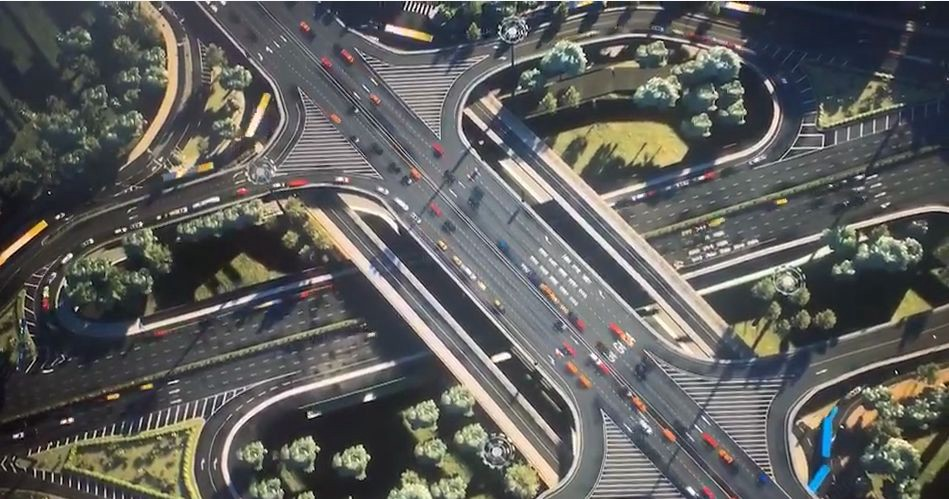
\includegraphics[scale=0.45]{figures/traffic_scene_digital_twin.jpeg}
	\caption{ تصویری از دوقلوی دیجیتال یک اتوبان در بیجینگ که به صورت زنده در حال شبیه‌سازی وضعیت کنونی اتوبان‌ است. \cite{51World:2019}}
	\label{fig:beijing_traffic_scene_dt}
\end{figure}

در \cref{fig:beijing_traffic_scene_dt}، تصویری از دوقلوی دیجیتال اتوبان بیجینگ غربی سوم\LTRfootnote{\lr{Beijing West 3rd Ring Road}} را مشاهده می‌کنیم. در این تصویر، دوقلوی دیجیتال صحنه ترافیکی علاوه بر مدل سه بعدی فضای شهری شامل خیابان‌ها و فضای سبز و دیگر المان‌های ثابت در صحنه، اطلاعات پویا مانند خودروهای در حال تردد را نیز شامل می‌شود.. حال با استفاده از این دوقلوی دیجیتال، می‌توان تراکم ترافیک در ساعات مختلف در این اتوبان دیجیتالی را به دست آورد. این اطلاعات کاربردهای متعددی می‌تواند داشته باشد. برای مثال، می‌توان از این اطلاعات بعنوان دادگانی برای آموزش مدل‌های یادگیری عمیق\LTRfootnote{\lr{Deep Learning}} استفاده کرد و تراکم ترافیک را در ساعات مختلف روز پیش‌بینی کرد. همان‌ طور که قبلاً نیز ذکر شد، دوقلوی دیجیتال می‌تواند دارای جریان دوطرفه اطلاعات باشد. به طور مثال در این اتوبان، داده‌های گرفته شده از حسگرهای مختلف همانند لایدارها\LTRfootnote{\lr{LiDAR Sensor}} و دوربین‌های مستقر (یا به عبارت دیگر یک آر.اس.یو\LTRfootnote{\lr{Road-Side Unit (RSU)}}) به عنوان ورودی دریافت می‌شوند (جریان داده دنیای واقعی به دوقلوی دیجیتال). پس از پردازش داده‌ها در دوقلوی دیجیتال و تشخیص خودروها و موقعیت مکانی آن در زمان‌های مختلف روز، مدل یادگیری عمیقی را توسعه دهیم که بتواند در راستای هوشمندسازی مدیریت ترافیک، زمان‌بندی چراغ‌های راهنمایی را بگونه‌ای کنترل کند که جریان ترافیکی بهینه شود (جریان داده‌ دوقلوی دیجیتال به دنیای واقعی).

\section{ضرورت استفاده از دوقلوی دیجیتال}
برخی از برتری‌های استفاده از دوقلوی دیجیتال به عنوان بستر شبیه‌سازی عبارتند از:

\begin{enumerate}
	\item \textbf{نزدیکی به واقعیت:} همانطور که ذکر شد، دوقلوی دیجیتال از مدل‌های پویا نیز بهره می‌برد و هدف آن نزدیکی به واقعیت تا حد امکان است. پس با مدل کردن یک صحنه ترافیکی براساس داده‌های بلادرنگ، می‌توان بستری برای سیستم‌های مدیریت ترافیک و خود‌رو‌های خودران مهیا کرد. نتایج آزمایش سیستم‌های طراحی شده در دوقلوی دیجیتال را می‌توان به دنیای واقعی نسبت داد زیرا عملا با آزمایش در دوقلوی دیجیتال، ما در بستری بسیار نزدیک به واقعیت سیستم‌ خود را آزمایش کرده‌ایم.
	\item \textbf{افزایش سرعت تحقیقات:} با بکارگیری از دوقلوی دیجیتال صحنه‌های ترافیکی، نیازی به تولید سناریو‌های مختلف ترافیکی وجود ندارد زیرا هر لحظه از دنیای واقعی در دوقلوی دیجیتال نیز در حال تشکیل است و به صورت خودکار سناریو‌های گوناگون رخ می‌دهند، در نتیجه سرعت تحقیقات و آزمایش سیستم‌های مدیریت ترافیک گوناگون به مراتب بیشتر است.
	\item \textbf{امنیت بالا:} در دوقلوی دیجیتال از مدل‌های پویا استفاده می‌شود، یعنی عابر پیاده و ماشین‌های دیگر نیز شبیه‌سازی می‌شوند و سیستم‌هایی هوشمند همچون ماشین‌های خودران و مدیریت ترافیک می‌توانند با وجود این مدل‌ها آزموده شوند. اما در دنیای واقعی آزمودن این در سطح شهر امری بسیار خطرناک است و ممکن است خسارات جبران ناپذیری بر سطح شهر وارد شود.
	\item \textbf{قابلیت پیش‌بینی بهتر:} با استفاده از دوقلوی دیجیتال، ما می‌توانیم ترافیک‌ را پیش‌بینی کنیم و نسبت به آن سیستم مدیریت ترافیک خود را تعلیم دهیم. به علت متصل بودن داده‌های دوقلوی دیجیتال به داده‌های دنیای واقعی، سناریو‌های گوناگون رخ می‌دهند و سیستم‌های مدیریت ترافیک داده‌های تمرینی بهتر و متنوع‌تر خواهند داشت \cite{singh2021digital}.
\end{enumerate}

\section{تعریف مسئله}
مشاهده کردیم که کشور چین، دوقلوی دیجیتال یکی از اتوبان‌های خود را در سال ۲۰۲۱ با موفقیت پیاده‌سازی کرد و در حال تحقیق بر روی این موضوع است. با الهام گرفتن از این پروژه، اهداف این پژوهش را در دو دسته‌ی هدف اصلی و اهداف فرعی بخش‌بندی می‌کنیم.

\subsection{هدف اصلی}

هدف اصلی این پروژه، پیاده‌سازی دوقلوی دیجیتالی از صحنه ترافیکی خیابان رشت، از دید درب رشت دانشگاه صنعتی امیرکبیر است. این دوقلوی دیجیتال به عنوان یک بازنمایی دقیق و پویا از خیابان رشت ایجاد می‌شود تا امکان شبیه‌سازی و مطالعه وضعیت‌های ترافیکی مختلف در این منطقه را فراهم کند. (مشابه دوقلوی دیجیتال اتوبان بیجینگ با جزییات به مراتب ساده‌تر)

\subsection{اهداف فرعی}

برای دستیابی به هدف اصلی پروژه، اهداف فرعی زیر تعیین شده‌اند:

\begin{enumerate}
\item مدل‌سازی ایستای سه‌بعدی خیابان رشت با استفاده از نرم‌افزارهای طراحی سه‌بعدی مبتنی بر برداشت داد‌ه‌های حسگر لایدار (به صورت دستی با کمک نرم‌افزارهای طراحی سه‌بعدی)
\item مستقر کردن حسگر‌های لایدار و دوربین در محل نگهبانی درب رشت دانشگاه صنعتی امیرکبیر به منظور برداشت داده‌های پویا.
\item پردازش داده‌های تصویر و ابر نقاط\LTRfootnote{\lr{Point Cloud (PCL)}} به منظور شناسایی و مکانیابی پدیده‌های پویا با استفاده از مدل‌های آماده یادگیری ماشین در زمینه تشخیص اجسام سه‌بعدی.
\item بصری‌سازی مدل سه‌بعدی ایستا و داده‌های پویای شناسایی شده در بستر سه‌بعدی با استفاده از شبیه‌ساز \lr{AWSIM}.
\item بصری‌سازی اطلاعات آماری بدست آمده از دوقلوی دیجیتال به منظور تجزیه و تحلیل نتایج پروژه.
\end{enumerate}

این اهداف فرعی به منظور دستیابی به هدف اصلی پروژه ارائه شده‌اند و با استفاده از آنها، پروژه به طور جامع توصیف و اجرا می‌شود.
\chapter{مفاهیم پایه و نگاهی بر کارهای پیشین}

\section{مفاهیم پایه}
برای آنکه درک مناسبی از مسئله‌ پیاده‌سازی دوقلوی دیجیتال و تشخیص اجسام پویا ایجاد شود، نیاز است که ابزار‌ها و الگوریتم‌هایی که در این پژوهش از آنها استفاده شده است به صورت اجمالی تعریف شوند.

\subsection{حسگرها}
حسگرها به عنوان اجزای ضروری در عرصه فناوری و جمع‌آوری داده‌ها، به عنوان چشم‌ها و گوش‌های سیستم‌های مختلف عمل می‌کنند. این دستگاه‌های الکترونیکی برای تشخیص و پاسخ به تغییرات فیزیکی یا محیطی طراحی شده‌اند و ظواهر جهان واقعی را به داده‌های قابل اندازه‌گیری تبدیل می‌کنند. حسگرها انواع گوناگونی دارند؛ از حسگرهای دما که تغییرات حرارتی را نظارت می‌کنند تا حسگرهای حرکت که حرکت را تشخیص می‌دهند. آنها در بسیاری از کاربردها مورد استفاده قرار می‌گیرند، از سیستم‌های خودرویی که ایمنی وسیله نقلیه را تضمین می‌کنند تا دستگاه‌های خانه هوش مصنوعی که راحتی و کارایی را افزایش می‌دهند. با توانایی در تجزیه و تحلیل داده‌ها به صورت بلادرنگ، حسگرها نقش اساسی در زمینه‌هایی مانند بهداشت، تولید، نظارت بر محیط زیست و موارد دیگر ایفا می‌کنند و تصمیم‌گیری آگاهانه و خودکارسازی فرآیندهای مختلف را در دنیای متصل ما امکان‌پذیر می‌سازند.

\subsubsection{حسگر لایدار}
لایدار یک اختصار برای تشخیص و فاصله‌سنجی با نور\LTRfootnote{\lr{LiDAR = Light Detection and Ranging}} است. در لایدار، نور لیزر از یک منبع (فرستنده) ارسال می‌شود و از اجسام حاضر در صحنه بازتاب می‌یابد. نور بازتاب شده توسط گیرنده سیستم تشخیص داده می‌شود و از زمان پرواز\LTRfootnote{\lr{TOF: Time of Flight}} این نور، برای توسعه نقشه فاصله\LTRfootnote{\lr{Distance Map}} اجسام استفاده می‌شود \cite{Synopsis:LiDAR}.


به طور اصولی، لایدار یک دستگاه اندازه‌گیری فاصله به هدف است که با ارسال یک پالس کوتاه نوری و ثبت زمان گذشته بین پالس نوری خروجی و تشخیص پالس نوری بازتابی (برگشتی)، فاصله را اندازه‌گیری می‌کند.

\begin{figure}[h]
	\centering
	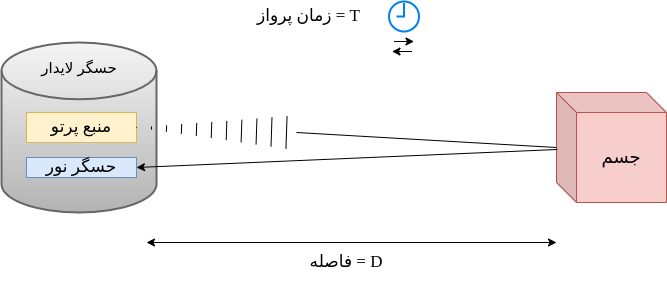
\includegraphics[scale=0.5]{figures/LiDAR_TOF.png}
	\caption{تصویری از نحوه محاسبه فاصله اجسام توسط حسگر لایدار}
	\label{fig:LiDAR_TOF}
\end{figure}

طبق \cref{fig:LiDAR_TOF}، با دانستن سرعت نور که با \lr{c} نمایش داده می‌شود داریم:
\begin{equation}\label{d=ct/2}
d = c \cdot t / 2
\end{equation}

یک سیستم لایدار ممکن است از آینه اسکن\LTRfootnote{\lr{Scan Mirror}}، چند پرتو لیزر یا ابزارهای دیگر برای اسکن فضای شیء استفاده کند. با توانایی ارائه اندازه‌گیری دقیق فواصل، لایدار می‌تواند برای حل مسائل متنوعی مورد استفاده قرار گیرد.

در حوزه حسگری از دور\LTRfootnote{\lr{Remote Sensing}}، سیستم‌های لایدار برای اندازه‌گیری پراکندگی، جذب یا بازتاب از ذرات یا مولکول‌های موجود در جو استفاده می‌شوند. برای این اهداف، سیستم‌ها ممکن است نیازهای خاصی در خصوص طول موج پرتوهای لیزری داشته باشند. می‌توان غلظت یک گونه مولکولی خاص در جو، به عنوان مثال متان و بار آئروسل\LTRfootnote{\lr{Aerosol Loading}} را اندازه‌گیری کرد. همچنین قطرات باران در جو می‌توانند اندازه‌گیری شوند تا فاصله یک توفان و نرخ بارندگی را تخمین بزنند.

سیستم‌های دیگر لایدار محور، مشخصات سطوح سه‌بعدی در فضای جسمی\LTRfootnote{\lr{Object Space}} را ارائه می‌دهند. در این سیستم‌ها، پرتوهای لیزری طیف خاص و مشخصی ندارند. به جای آن، ممکن است طول موج پرتوهای لیزری برای اطمینان از ایمنی چشمی یا جلوگیری از ویژگی‌های طیفی جو انتخاب شود. پرتوی مورد ارزیابی برخورد کرده و توسط یک "هدف سفت" به سمت گیرنده لایدار بازتاب می‌شود.

\begin{figure}[h]
    \centering
    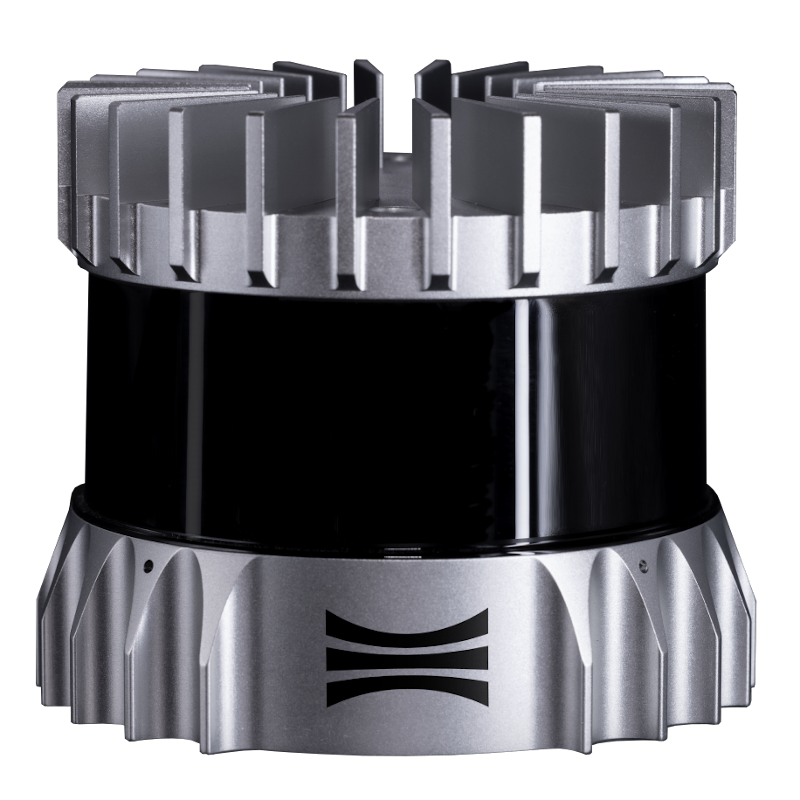
\includegraphics[width=0.25\linewidth]{figures/OS1_64_LiDAR.png}
    \caption{حسگر لایدار \lr{OS1:64} از شرکت \lr{Ouster} \cite{Ouster:LiDAR_Specification}}
    \label{fig:OS1_64_LiDAR}
\end{figure}

لایدار همچنین می‌تواند برای تعیین سرعت یک جسم هدف، مورد استفاده قرار گیرد. این کار می‌تواند به وسیله تکنیک داپلر\LTRfootnote{\lr{Doppler Technique}} یا اندازه‌گیری فاصله تا یک هدف در مدت زمان کوتاهی انجام شود. به عنوان مثال، سرعت باد جوی و سرعت یک خودرو می‌تواند توسط یک سیستم لایدار اندازه‌گیری شود.

علاوه بر این، سیستم‌های لایدار می‌توانند برای ایجاد مدل سه‌بعدی از یک صحنه پویا مورد استفاده قرار گیرند، همانند صحنه‌هایی که یک خودروی خودران با آن مواجه می‌شود. این کار در روش‌های مختلفی قابل انجام است اما معمولاً با استفاده از تکنیک‌های اسکن‌کردن ۳۶۰ درجه و محسابه زمان پرواز صورت می‌گیرد.

در حال حاضر، به طور متداول برای ایجاد مدل سه‌بعدی از دنیای اطراف حسگر لایدار مورد استفاده قرار می‌گیرد. سیستم‌های مسیریابی خودکار از سیستم‌هایی است که از ابر نقاط ایجاد شده توسط حسگر لایدار استفاده می‌کند. برخلاف تصاویر، ابر نقاط پراکنده هستند: نمونه‌ها به طور یکنواخت در فضا توزیع نشده‌اند. لایدارها به عنوان حسگرهای فعال، نیازی به نور محیطی ندارند و از این رو می‌توان با توجه به شرایط آب و هوایی نامساعد، تشخیص قابل اعتمادتری انجام داد \cite{arnold2019survey}. سیستم‌های کوچکتر لایدار حتی در دستگاه‌هایی با اندازه‌های کوچک مانند تلفن‌های همراه نیز یافت می‌شوند.

\subsubsection{دستگاه \lr{RSU}}
\lr{RSU}\LTRfootnote{\lr{Roadside Unit}}یک گیرنده و فرستنده است که عموما در کنار خیابان‌ها و خطوط عابرپیاده مستقر می‌شود. این دستگاه‌ها می‌توانند بر روی یک خوردرو نیز مستقر شوند و یا با دست حمل شوند اما تنها زمانی شروع به کار کردن می‌کند که ثابت باشد و در حال حرکت نباشد. \lr{RSU}ها تنها در منطقه‌ای که مجوز آن‌ را داشته باشند می‌توانند عمل کنند. اما آنهایی که توسط دست نیز حمل می‌شوند، می‌توانند بدون مجوز در منطقه‌هایی که تداخلی با بقیه \lr{RSU}های دارای مجوز و دولتی ندارند، عمل کنند. این دستگاه‌ها داده‌‌های ترافیکی و آب‌وهوایی را به سیستم‌های مدیریت کلان شهری می‌فرستند و همچنین از آنها اطلاعات می‌گیرند. همچنین دستور‌هایی را می‌توانند به ماشین‌ها بدهند تا از خطر احتمالی و یا  ترافیک احتمالی جلوگیری شود. در این پژوهش منظور از \lr{RSU}،  حسگر لایداری است که در کنار خیابان مستقر شده است.

\subsection{شبکه‌های عصبی}
یادگیری ماشین\LTRfootnote{Machine Learning (ML)} یک روش موثر برای رسیدن به اهداف هوش‌مصنوعی است و روش‌های متعددی برای آموزش ماشین جهت دسته‌بندی و پیش‌بینی ارائه شده است. در میان این روش‌ها، یادگیری عمیق با استفاده از شبکه‌ی عصبی به نتایج فوق‌العاده‌ای در انواع کارها مانند پردازش تصویر، تشخیص چهره و غیره دست‌ یافته است. شبکه‌ی عصبی مجموعه‌ای از الگوریتم‌ها است که تلاش می‌کند تا روابط زیربنایی را در مجموعه‌ای از داده‌ها از طریق فرایندی که نحوه‌ی عملکرد مغز انسان را تقلید می‌کند، تشخیص دهد \cite{zhou2019edge}. 

از آن جا که شبکه‌ی عصبی\LTRfootnote{Neural Networks} در یادگیری عمیق، شامل چندین لایه است، به آن شبکه‌ی عصبی عمیق اطلاق می‌شود. همان‌طور که در \cref{fig:standard_nn} مشاهده می‌شود هر لایه در شبکه‌ی عصبی عمیق از نورون‌هایی تشکیل شده است که قادرند بر اساس داده‌ی ورودی، خروجی غیرخطی تولید نمایند.

\begin{figure}[h]
    \centering
	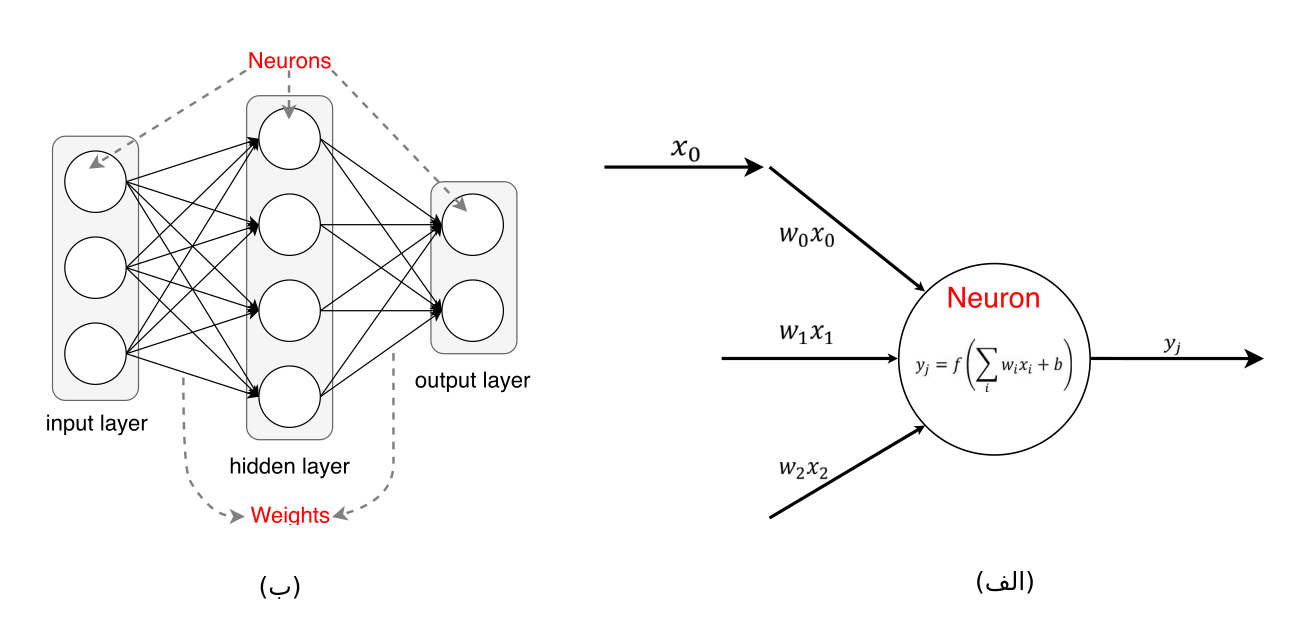
\includegraphics[width=1\linewidth]{figures/standard_nn.png}
	\caption{مدل استاندارد شبکه‌ی عصبی عمیق \cite{zhou2019edge}}
	\small\textsuperscript{عصبی عمیق شبکه‌ی لایه‌های (ب) نورون یک معماری (الف)}
	\label{fig:standard_nn}
\end{figure}

\subsubsection{شبکه‌های عصبی پیچشی}

شبکه‌های عصبی پیچشی\LTRfootnote{Convolutional Neural Network (CNN)} یا به‌اختصار شبکه‌های پیچشی، دسته‌ای از شبکه‌های عصبی مصنوعی هستند که از دیگر شبکه‌های عصبی در کاربردهایی با ورودی‌های سیگنال تصویر، گفتار یا صوتی عملکرد بهتری نشان می‌دهند و معماری آن‌ها از سازمان‌دهی قشر بینایی حیوانات الهام گرفته شده است.  در این مدل، لایه‌ها با استفاده از تابع پیچش\LTRfootnote{\lr{Convolution}}، ویژگی‌های ساده ورودی را استخراج می‌کنند. فیلترهای پیچشی در این مدل سهم زیادی در نمایش سطح بالای داده‌های ورودی داشته‌اند و در این معماری شبکه مستقیما از داده‌ها یاد می‌گیرد و نیاز به استخراج دستی ویژگی را از بین می‌برد. یک نمونه از این شبکه‌ها که برای طبقه‌بندی عکس از آن استفاده شده است در \cref{fig:standard_cnn} قابل ‌مشاهده است. این نوع شبکه‌ی عصبی معمولا دارای سه ‌لایه‌ی اصلی است که عبارت‌اند از: 

\begin{enumerate}
	\item لایه‌ی پیچش
	
	\item لایه‌ی ادغام\LTRfootnote{\lr{Pooling Layer}}
	
	\item لایه‌ی تماما متصل\LTRfootnote{\lr{Fully-connected Layer}}
\end{enumerate}

\begin{figure}[h]
    \centering
    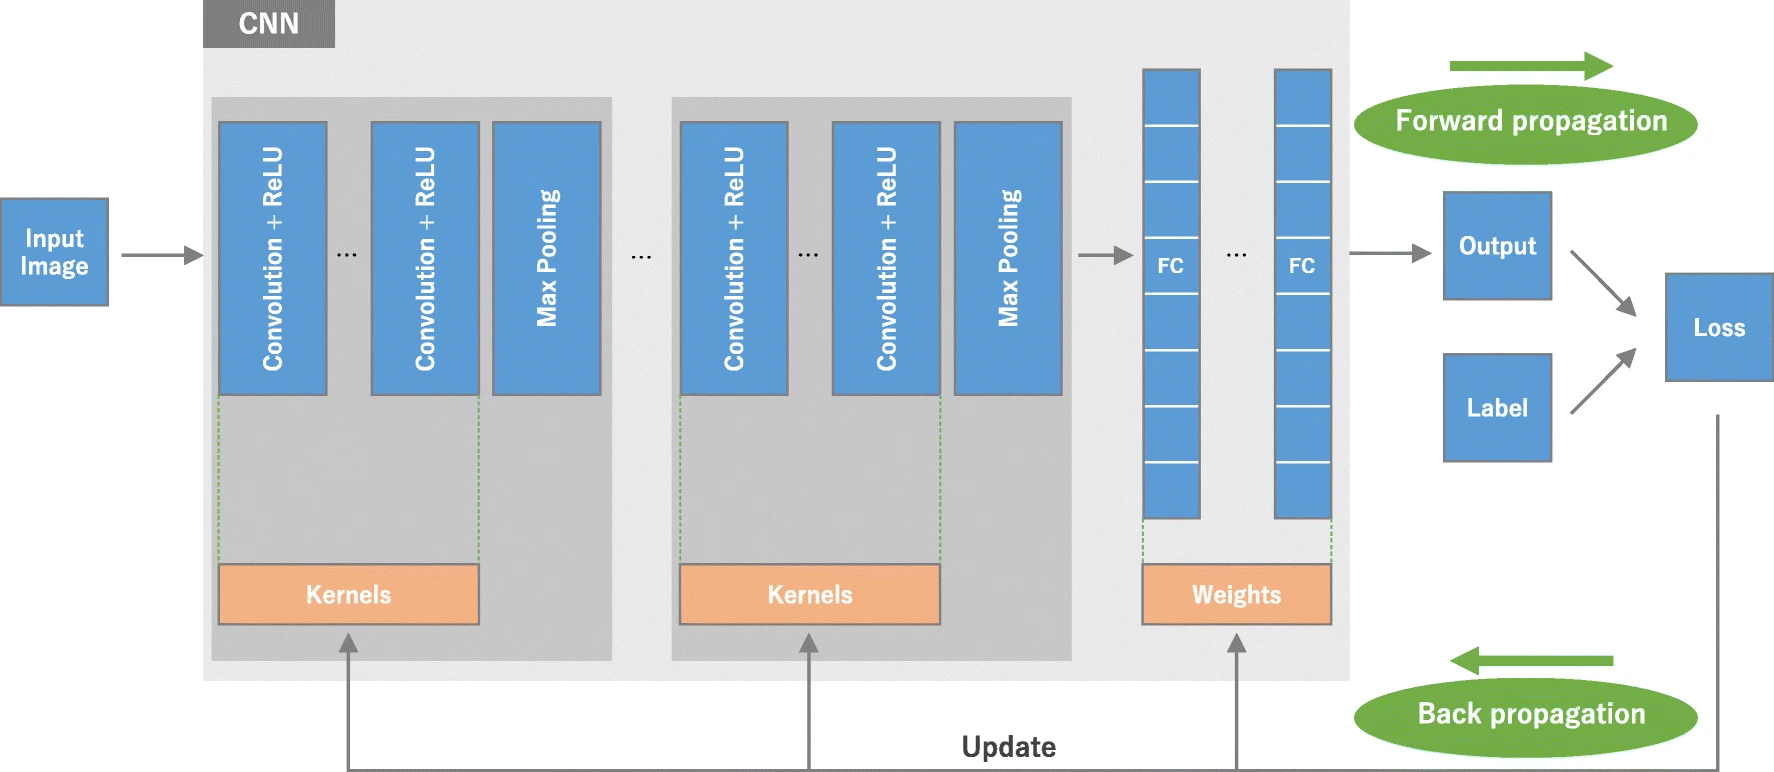
\includegraphics[width=1\linewidth]{figures/standard_cnn.png}
    \caption{نگاهی کلی به معماری استاندارد شبکه‌های پیچشی \cite{yamashita2018convolutional}}
    \label{fig:standard_cnn}
\end{figure}

دو لایه‌ی اول و دوم که لایه‌های پیچش و ادغام هستند، استخراج ویژگی را انجام می‌دهند. در حالی که لایه‌ی سوم، ویژگی‌های استخراج شده را در خروجی نهایی، نگاشت می‌کند یا به عبارتی دیگر از ویژگی‌های استخراج شده، استنتاج می‌کند. لایه‌ی پیچشی نقش کلیدی را در شبکه‌های پیچشی ایفا می‌کند، که از مجموعه‌ای از  عملیات ریاضی، نظیر پیچش تشکیل شده است \cite{yamashita2018convolutional}.

\subsubsection{لایه‌ پیچش}

 لایه پیچش از اجزای اساسی معماری شبکه‌های عصبی پیچشی است که عملیات استخراج ویژگی را انجام می‌دهد. این عملیات به طور معمول شامل ترکیبی از عملیات خطی و غیرخطی، یعنی عملیات پیچش و تابع فعال‌سازی می‌شود.

پیچش یک عملیات ویژه خطی است که برای استخراج ویژگی‌ها استفاده می‌شود. در این عملیات، یک ماتریس کوچک از اعداد به نام هسته یا فیلتر\LTRfootnote{\lr{Kernel (Filter)}}، بر روی ورودی اعمال می‌شود. ورودی نیز یک ماتریس از اعداد به نام تنسور\LTRfootnote{\lr{Tensor}} است. با قرار گرفتن فیلتر بر روی هر بخش از تنسور، اعداد فیلتر درایه به درایه در مولفه‌های تنسور متناظر ضرب می‌شوند و در نهایت همه اعداد با هم جمع می‌شوند تا یک نقشه ویژگی\LTRfootnote{\lr{Feature Map}} شکل بگیرد. اگر یک تنسور دوبعدی از یک تصویر به نام \lr{I} و یک فیلتر به نام \lr{k} داشته باشیم، عملیت پیچش طبق فرمول زیر انجام می‌شود:
\begin{equation}
    \sum_{m}\sum_{n} i(m, n)k(i-m, j-n)
\end{equation}
این پروسه با فیلترهای مختلف تکرار می‌شود که هر کدام ویژگی‌های مختلفی از تنسور را استخراج می‌کنند.\begin{figure}[h!]
    \begin{minipage}{0.5\textwidth}
        \centering
        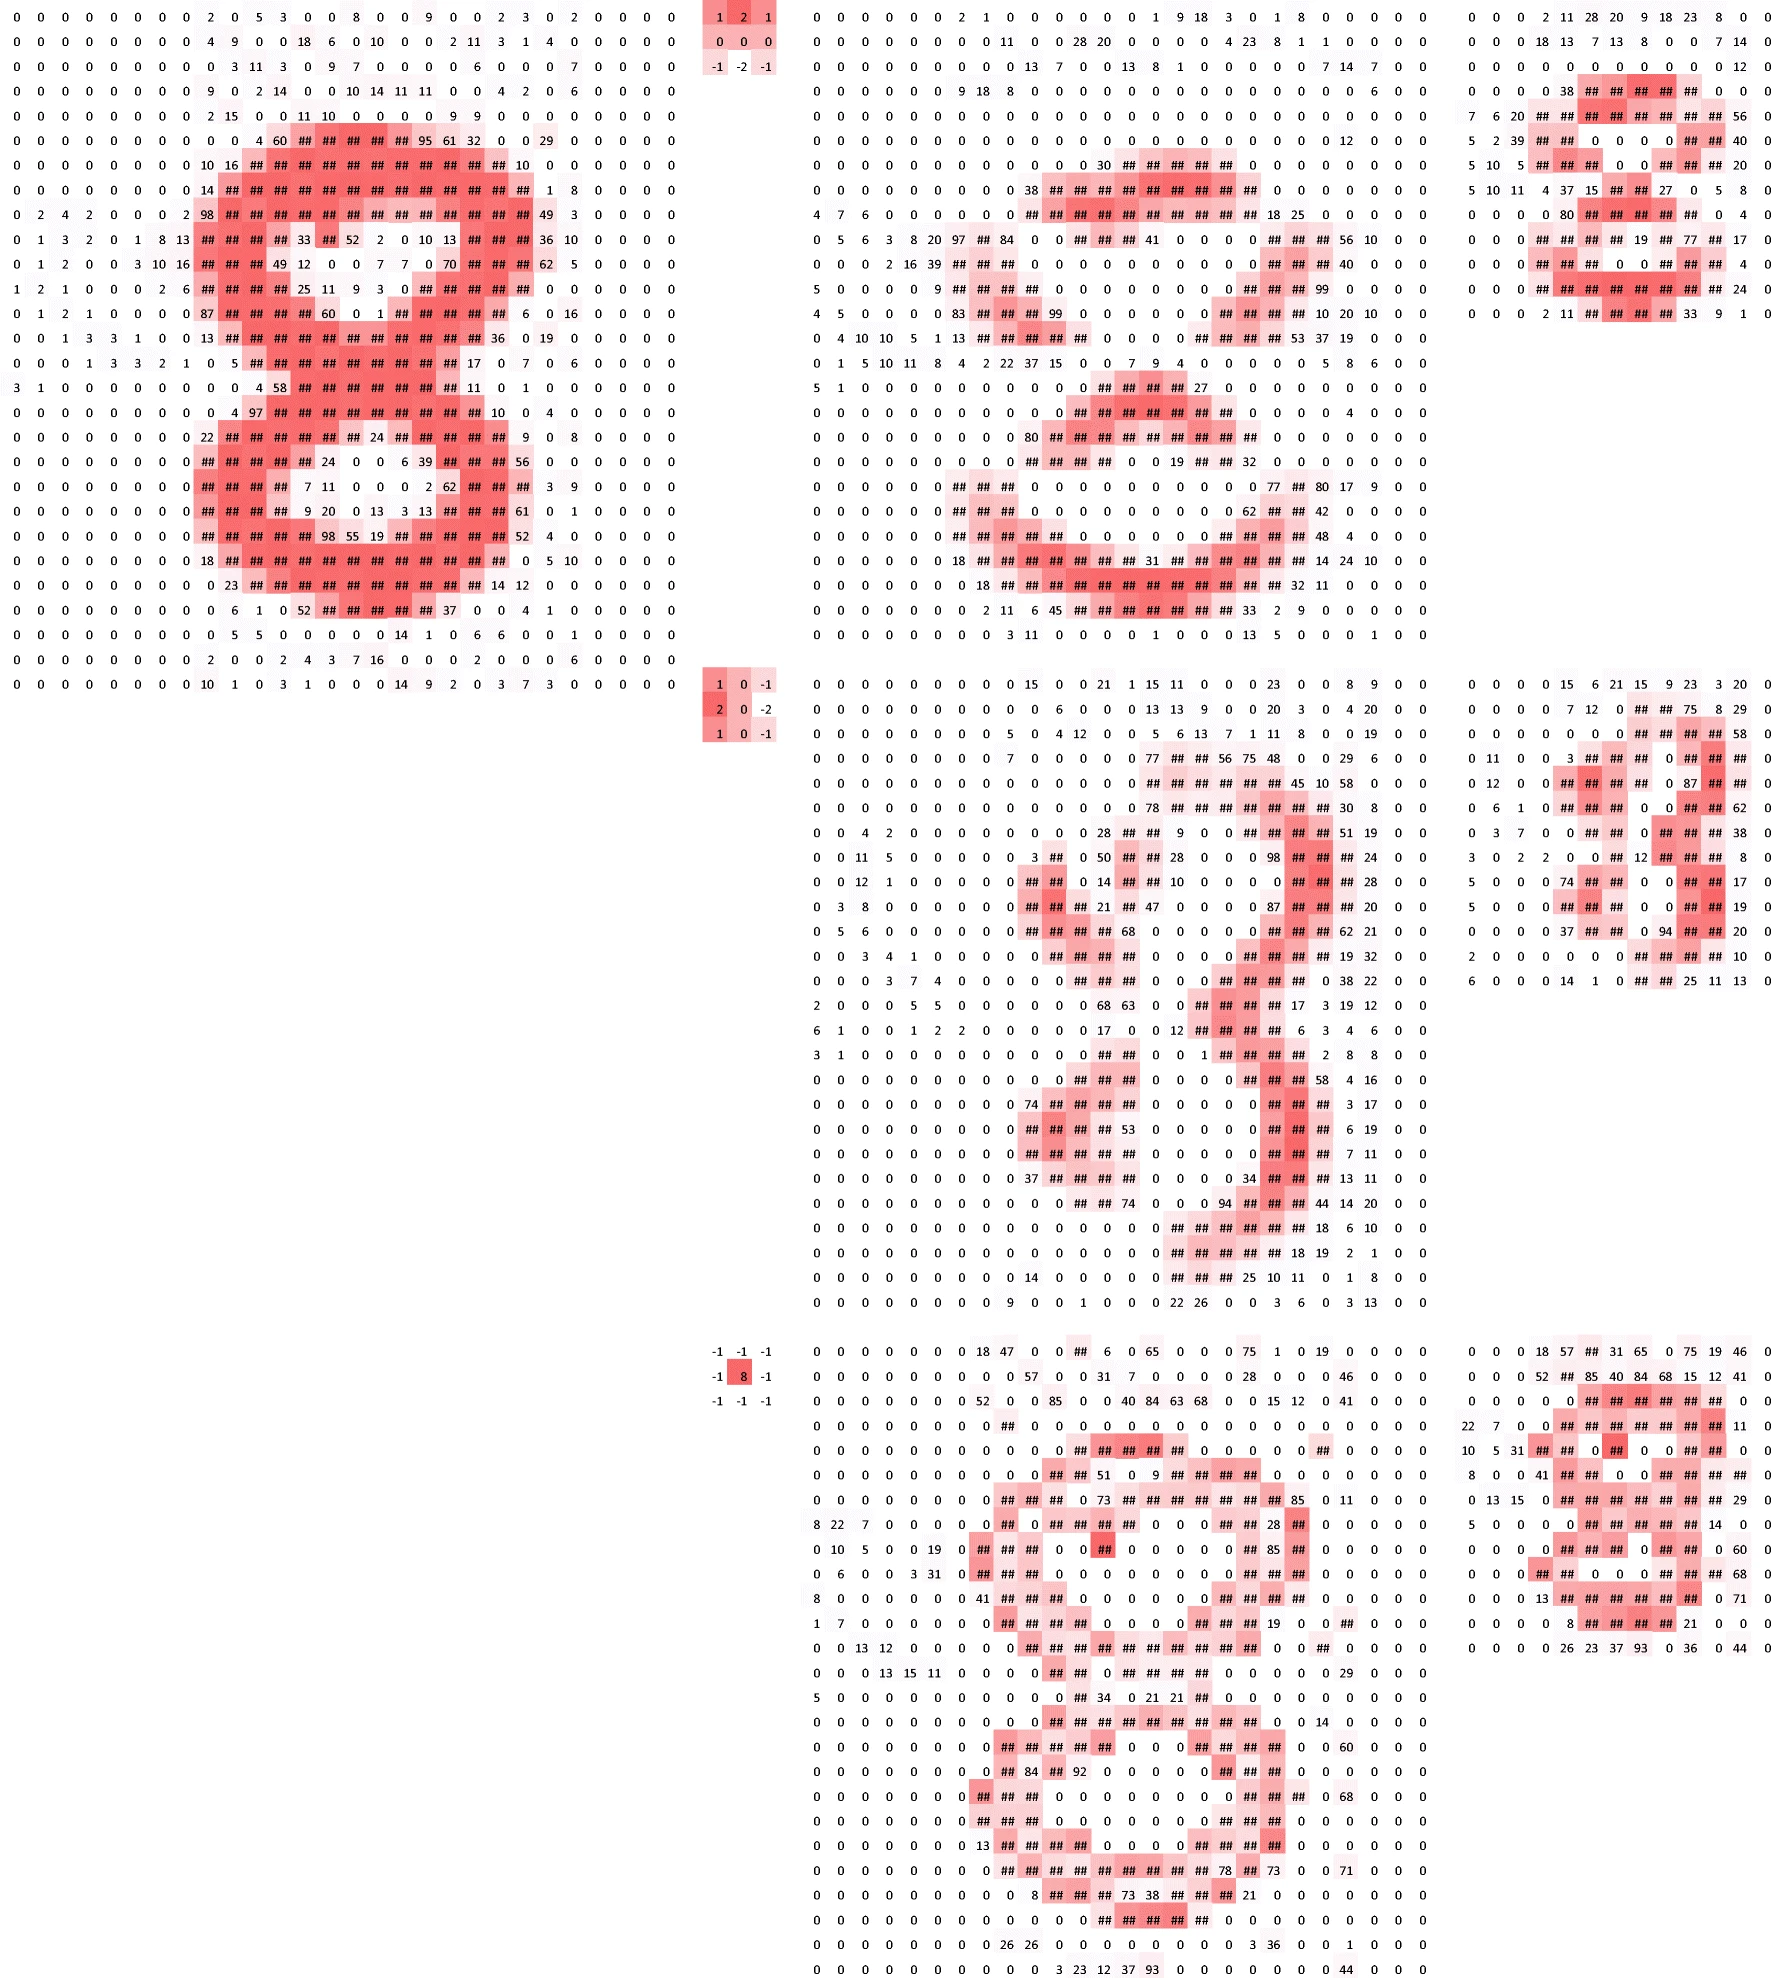
\includegraphics[width=1\linewidth]{figures/Feature_Map.png}
    \end{minipage}
    \hspace{0.3cm}
    \begin{minipage}{0.5\textwidth}
        \centering
        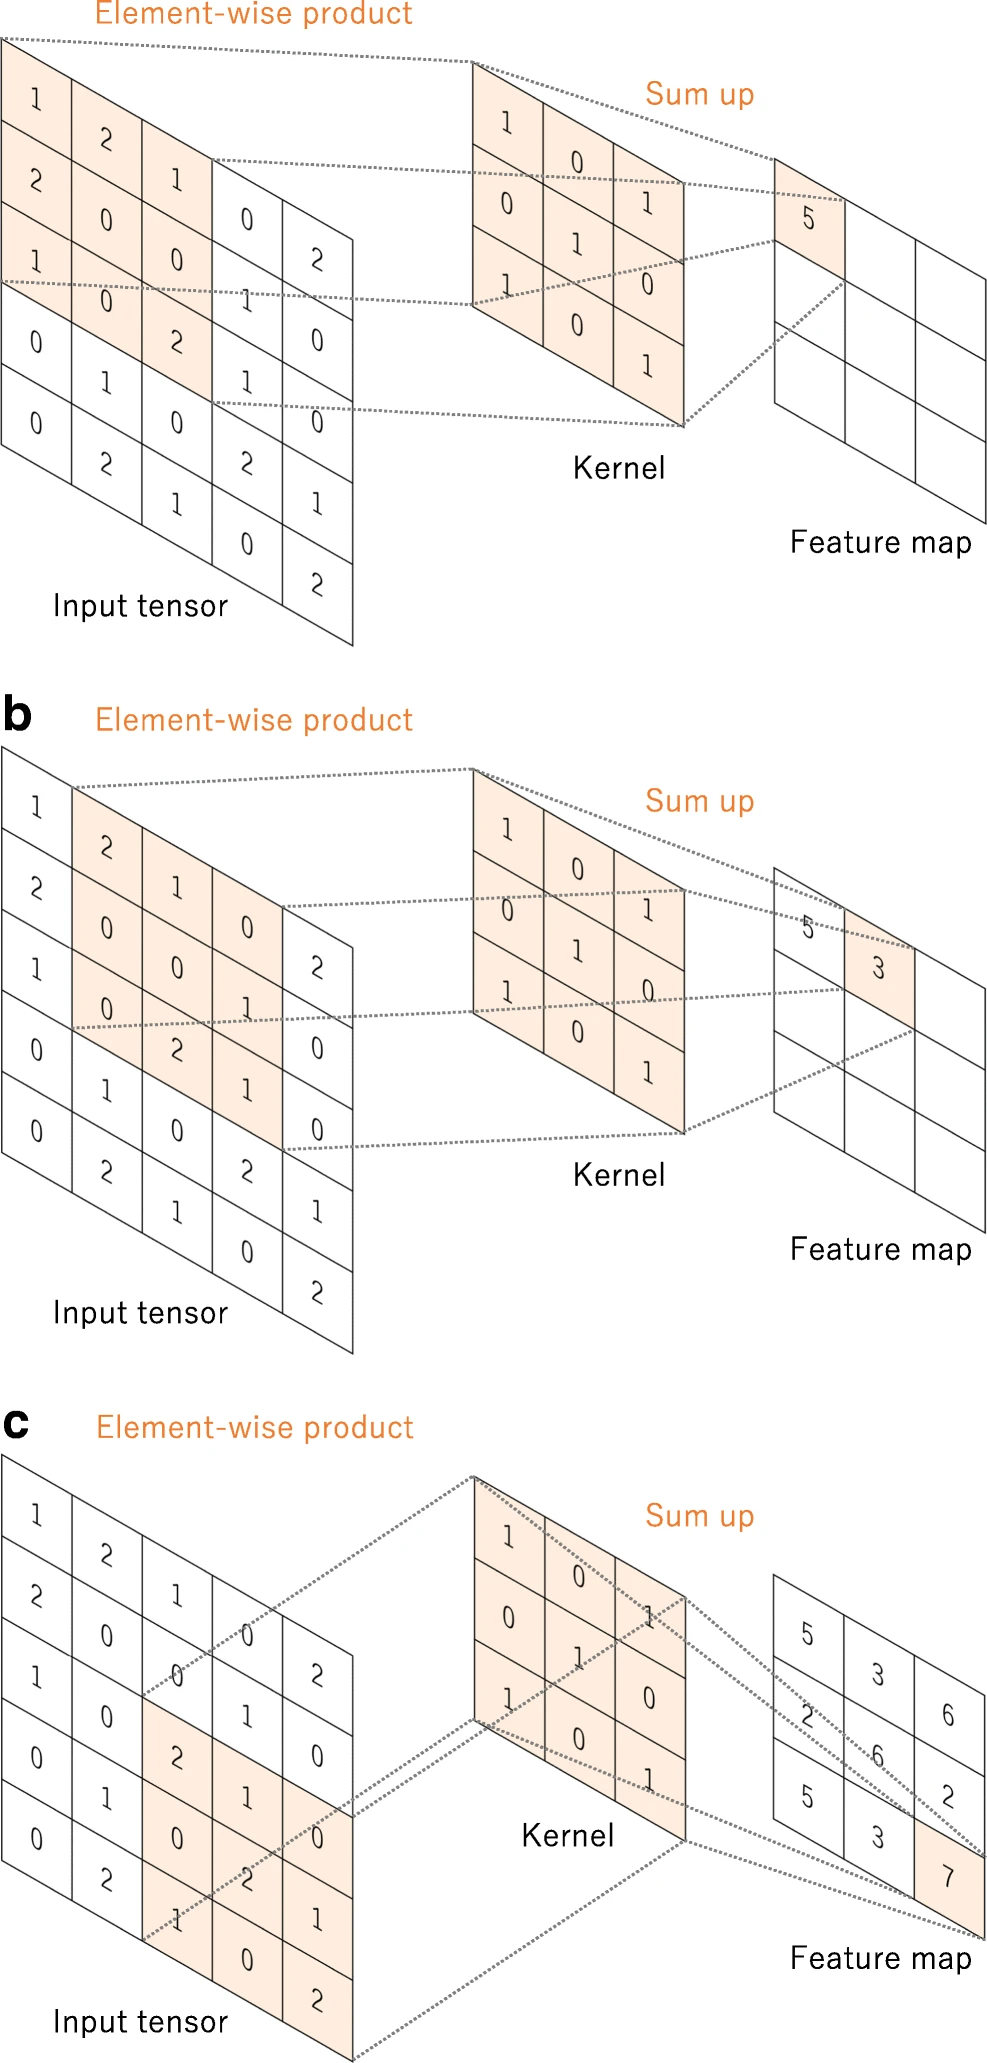
\includegraphics[width=0.9\linewidth]{figures/Convolution_Procedure.png}
    \end{minipage}
    \begin{center}
        \caption{عملیت پیچش با فیلترهای ۳ $\times$ ۳ و گام‌ ۱ \cite{yamashita2018convolutional}}
        \small\textsuperscript{می‌کنیم. مشاهده را مختلف فیلترهای ویژگی نقشه‌های شکل،  راست سمت در}
    \end{center}
    \label{fig:convolution_procedure}
\end{figure} ابرپارامتر‌هایی\LTRfootnote{\lr{Hyperparameter}} که نتیجه عملیات پیچش را تحت تاثیر قرار می‌دهند، ابعاد و تعداد ماتریس‌های فیلتر است. عموما ابعاد فیلترها ۳ $\times$ ۳ است، اما بعضی اوقات از ابعاد ۵ $\times$ ۵ و ۷ $\times$ ۷ نیز استفاده می‌شود. تعداد فیلترها عموما دلخواه است و عمق نقشه‌های ویژگی را تحت تاثیر قرار می‌دهد.

عملیات پیچشی که در \cref{fig:convolution_procedure} دیده‌ می‌شود، نمی‌گذارد که ماتریس فیلتر از ماتریس تنسور خارج شود. در واقع نقطه مرکز فیلتر هیچ‌گاه بر روی درایه‌های گوشه‌ای تنسور قرار نمی‌گیرد. این باعث می‌شود که ابعاد نقشه‌ی ویژگی‌ حاصل، کوچک‌تر از ابعاد تنسور باشد. لایه‌گذاری‌\LTRfootnote{\lr{Padding}}، که معمولا لایه‌گذاری صفر‌\LTRfootnote{\lr{Zero Padding}} است، یک روش برای حل این مشکل است. در این روش سطرها و ستون‌های تماما صفر به دور ماتریس تنسور اضافه می‌شوند. با این کار، مرکز فیلتر بر روی مولفه‌های گوشه ماتریس نیز جای می‌گیرد و نقشه ویژگی حاصل، هم‌اندازه تنسور خواهد شد. عموم مدل‌های عمیق شبکه‌های پیچشی، از لایه‌های پیچش زیادی استفاده می‌کنند و اگر از تکنیک لایه‌گذاری صفر استفاده نکنند، نقشه ویژگی آنها کوچکتر و کوچکتر می‌شود و عملا بدرد نخواهد خورد.

\begin{figure}[h!]
    \centering
    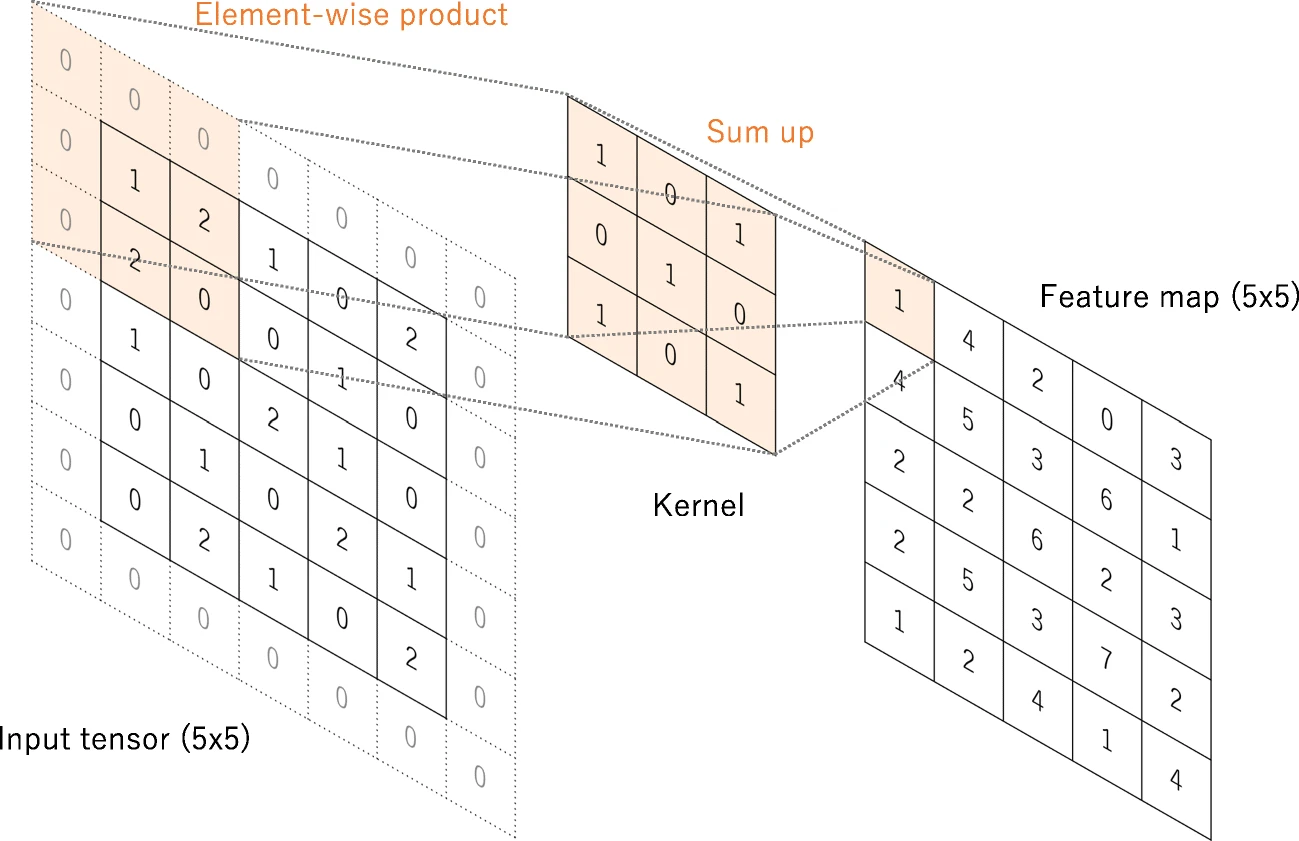
\includegraphics[width=1\linewidth]{figures/Zero_Padding.png}
    \caption{یک عملیات پیچش با لایه‌گذاری صفر \cite{yamashita2018convolutional}}
    \label{fig:zero_padding}
\end{figure}

طبق \cref{fig:zero_padding}، مشاهده می‌کنیم که با لایه‌گذاری صفر، ابعاد نقشه ویژگی هم اندازه تنسور ورودی است. اما بایستی دقت کرد که برای فیلتر‌های بزرگ‌تر و گام‌های\LTRfootnote{\lr{Stride}} بیشتر، نیاز به لایه‌گذاری صفر بیشتری خواهیم داشت. به فاصله بین دو عملیات اعمال فیلتر در یک سطر را گام می‌گویند. اندازه گام عموما ۱ است، اما گام‌های بیشتر از ۱ نیز در مواقعی که نیاز به نمونه‌کاهی\LTRfootnote{\lr{Downsampling}} نقشه ویژگی باشد، استفاده می‌شود. عملیات پیچش سه‌بعدی نیز به همین شکل است با این تفاوت که فیلترها سه‌بعدی هستند و در راستای عمق تنسور سه‌بعدی ورودی نیز حرکت می‌کنند.
\\
شبکه‌های عصبی پیچشی، دارای دامنه‌ی گسترده‌ای از کاربردها هستند و به خارج از تشخیص تصویر\LTRfootnote{\lr{Image Recognition}} گسترش یافته‌اند. از یادگیری سلسه‌وار ویژگی‌های آنها نیز در پردازش زبان طبیعی\LTRfootnote{\lr{Natrual Language Processing (NLP)}} و تجزیه و تحلیل گفتار\LTRfootnote{\lr{Speech Recogntion}} بهره‌برداری می‌شود. علاوه بر این، شبکه‌های عصبی پیچشی جلو‌دار تازه‌ترین پیشرفت‌ها در خودروهای خودران بوده‌اند، جایی که داده‌ها از حسگرهایی مانند لایدار و دوربین‌ها پردازش می‌شود، تا تصمیم‌گیری بلادرنگ در سناریو‌های مختلف رانندگی را ممکن کند. با توسعه مداوم معماری‌های شبکه‌های عصبی پیچشی و تکنیک‌های بهینه‌سازی، قابلیت‌های آنها برای مقابله با وظایف به تدریج پیچیده‌تر، گسترش یافته است. با پیشرفت تکنولوژی، شبکه‌های عصبی پیچشی همچنان در خط مقدم تحقیقات هوش مصنوعی قرار دارند و توانایی بی‌نظیری را ارائه می‌دهند تا جنبه‌های مختلفی از زندگی روزمره ما را بهبود دهند و اتوماسیون بخش‌های مختلفی از زندگی را امکان‌پذیر کنند.

\subsection{ابر نقاط و تشخیص اجسام سه‌بعدی}

در مدل‌سازی سه‌بعدی، ابر نقاط مجموعه‌ای از داده‌های نقطه‌ای در یک سیستم مختصات سه‌بعدی است که به طور معمول به عنوان دستگاه مختصات کارتزین\LTRfootnote{\lr{Cartesian Coordinate System}} یا محورهای \lr{XYZ}  شناخته می‌شود.
هر نقطه نمایانگر یک اندازه‌گیری
\begin{figure}[h]
    \centering
    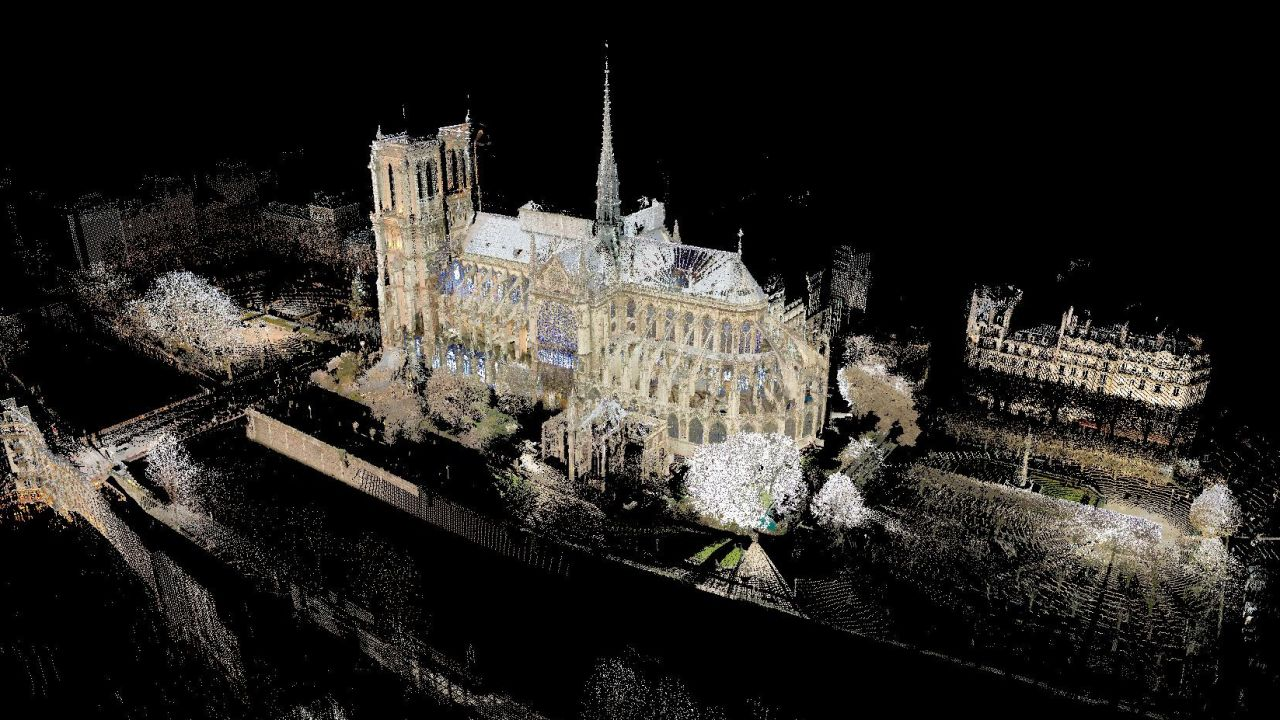
\includegraphics[width=0.84\linewidth]{figures/notre_dame_lidar_scan.png}
    \caption{اسکن رنگی لایدار از ساختمان معروف نوتردام پاریس که با استفاده از آن این ساختمان را بازسازی کردند.}
    \label{fig:notre_dame_lidar}
\end{figure}
فضایی واحد بر روی سطح شیء است. با تجمع این نقاط، ابر نقاط کل سطح خارجی یک شیء را می‌تواند نمایان کند. اگر مقادیر رنگ هر نقطه نیز اندازه‌گیری شود، اطلاعات رنگی نیز می‌تواند به ابر نقاط افزوده شود.
\begin{figure}[h]
    \centering
    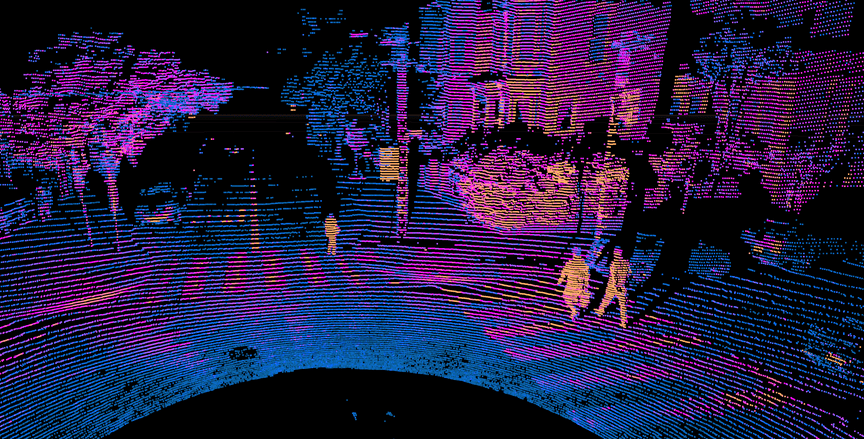
\includegraphics[width=0.84\linewidth]{vehicle_lidar_scan.png}
    \caption{اسکن لایدار \lr{OS1:64} از شرکت \lr{Ouster} که بر روی یک ماشین نصب شده است.}
    \label{fig:vehicle_lidar_scan}
\end{figure}
ابر نقاط با استفاده از یک اسکنر سه‌بعدی، لایدار یا نرم‌افزار فتوگرامتری\LTRfootnote{\lr{Photogrammetry}} ایجاد می‌شود.

در حوزه‌ی خودروهای خودران و سیستم‌های مدیریت هوشمند ترافیک نیز از لایدارها استفاده می‌شود تا ابر نقاط حاصل از فضای دور ماشین یا جاده‌ها به عنوان ورودی به مدل‌های هوش مصنوعی داده شود و اجسام داخل این فضا شناسایی شوند.

\subsubsection{تشخیص اجسام سه‌بعدی}
ادراک فضای سه‌بعدی یک پیش‌نیاز در حوزه رانندگی خودکار و دوقلوی دیجیتال است. درک کامل از آنچه که در حال حاضر در جلوی حسگر رخ می‌دهد، تسهیل‌دهنده‌ای برای اجزای پایین-دست\LTRfootnote{\lr{Downstream}} است تا به موقع واکنش نشان دهند. این همان چیزی است که تشخیص اجسام سه‌بعدی\LTRfootnote{\lr{3D Object Detection}} را هدف قرار می‌دهد.
\begin{figure}[h]
    \centering
    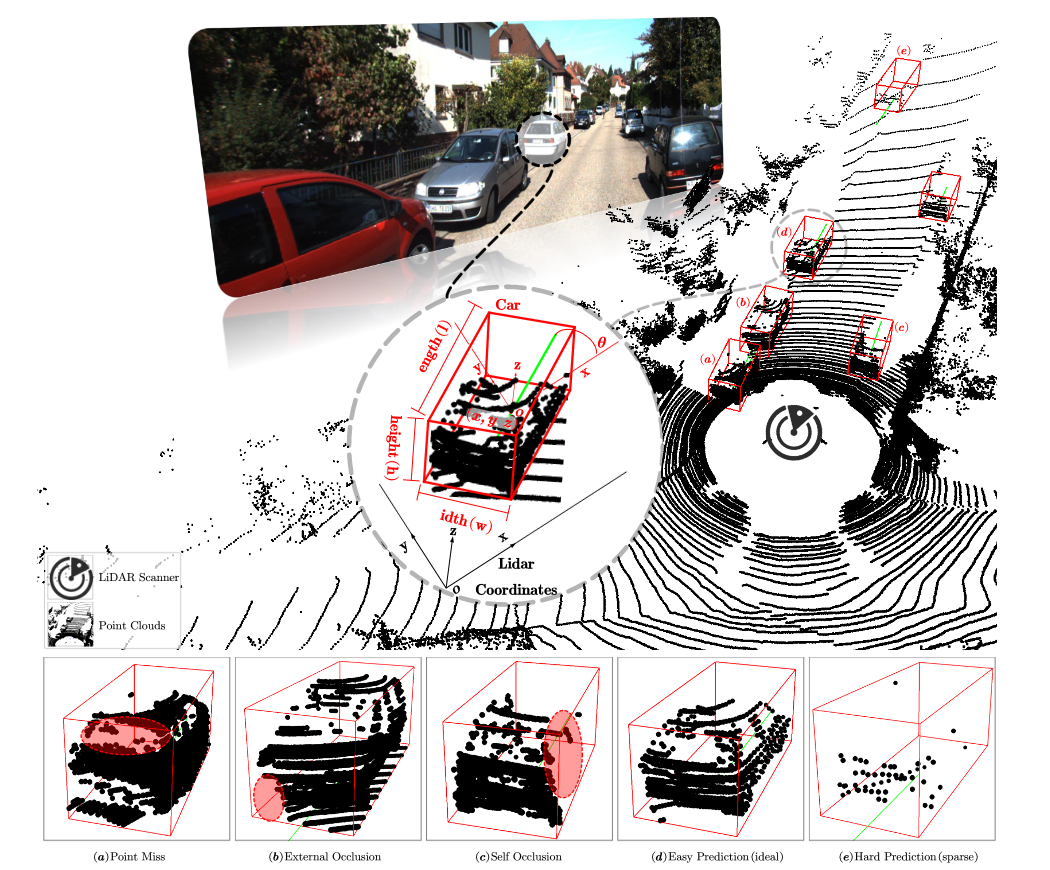
\includegraphics[width=1\linewidth]{figures/3D_Object_Detection_Overview.png}
    \caption{بررسی اجمالی وظیفه‌ی تشخیص اجسام سه‌بعدی از تصاویر و ابر نقاط\cite{qian20223d}}
    \label{fig:3d_object_detection_overview}
\end{figure}تشخیص اجسام سه‌بعدی، فضای اطراف ما را از طریق اختصاص یک برچسب\LTRfootnote{\lr{Label}}، تعیین شکل اجسام با کشیدن کادر محصورکننده\LTRfootnote{\lr{Bounding Box}}، و اعلام فاصله اجسام از حسگر توصیف می‌کند. علاوه بر این، تشخیص سه‌بعدی حتی زاویه‌ی جهت‌گیری\LTRfootnote{\lr{Orientation}} اجسام را به ما می‌دهد. این اطلاعات بدست‌ آمده از پشته‌ی ادراک\LTRfootnote{\lr{Detection Stack}}، این امکان را فراهم می‌کند که مدل‌های برنامه‌ریزی پایین-دست تصمیم‌گیری کنند \cite{qian20223d}.

\cref{fig:3d_object_detection_overview} یک بررسی اجمالی از تشخیص اجسام سه‌بعدی با استفاده از ابر نقاط و تصویر را نشان می‌دهد.
مشاهده می‌کنیم که چالش‌هایی در تشخیص اجسام سه‌بعدی داریم:
\begin{itemize}
    \item \lr{a}) عدم دریافت نقطه:‌ هنگامی که سیگنال‌های لایدار نتوانند از سطح شئ بازتاب شوند و به حسگر برگردند.
    \item \lr{b}) مسدودی از بیرون:‌ هنگامی که سیگنال‌های لایدار توسط موانع اطراف مسدود شوند.
    \item \lr{c}) مسدودی از درون: هنگامی که طرف نزدیک شئ طرف دیگر آنرا مسدود کند، که ابر نقطه جسم را در عمل به ابر نقطه‌ای ۵.۲ بعدی تبدیل می‌کند. 
\end{itemize}
مشاهده می‌کنیم که پیش‌بینی کادر محصورکننده‌ در مورد \lr{(d)} به مراتب آسان‌تر از مورد \lr{(e)} است؛ زیرا اجسامی که در فواصل دورتر از لایدار هستند، نقاط پراکنده و به اصطلاح تنک‌تری\LTRfootnote{\lr{Sparse}} دارند.

هدف اصلی تشخیص اجسام سه‌بعدی، تشخیص اجسام با ایجاد کادر محصور‌کننده سه‌بعدی و اختصاص برچسب به آنها است. برای حل این مسئله دو مدل متداول تشخیص اجسام سه‌بعدی، یعنی تصاویر و ابر نقاط، با چالش‌های مختلفی روبرو می‌شوند. با استفاده تنها از تصاویر، چالش اصلی عدم وجود اطلاعات عمق اجسام است؛ زیرا با وجود پیشرفت‌های زیاد در زمینه بازیابی عمق از تصاویر، این مسئله هنوز یک مسئله با پیچیدگی بالا و حل نشده محسوب می‌شود. همچنین، یک شئ در وضعیت‌های سه‌بعدی مختلف ممکن است به نمایش‌های تصویری مختلفی منجر شود، که برای یادگیری نمایش کادرها سودمند نیست. علاوه بر این، از آنجا که دوربین حسگری غیرفعال\LTRfootnote{\lr{Passive Sensor}} است، تصاویر طبیعتا نسبت به روشنایی (به عنوان مثال در شب) یا شرایط جوی (هوای بارانی) تاثیرپذیرند. از سوی دیگر، با استفاده تنها از ابر نقاط، مواجهه با چالش‌های مربوط به یادگیری بازنمایی\LTRfootnote{\lr{Representation Learning}} کادر محصورکننده‌ی اجسام رخ می‌دهد. طبیعت ابر نقاط، بی‌نظمی و تنک بودن است، به همین دلیل اعمال پیچش بر روی آن، منجر به "از دست رفتن اطلاعات شکل و واریانس در ترتیب نقاط" می‌شود. به علاوه، ابر نقاط در عمل دو و نیم‌بعدی هستند که مشکلات آن در \cref{fig:3d_object_detection_overview} قابل مشاهده است. با حذف المان استفاده از شبکه‌های عصبی پیچشی، یک راه برای نمایش ابر نقاط، نمایش آنها به عنوان شبکه‌ای از واکسل‌ها\LTRfootnote{\lr{Voxel Grid}} می‌باشد. معضل این روش این است که افزایش اندازه مکعب واکسل، باعث از دست دادن وضوح و به تبع آن کاهش دقت مکان‌یابی می‌شود؛ در حالی که کاهش اندازه آن، پیچیدگی و استفاده از حافظه را افزایش می‌دهد. راه دیگر نمایش ابر نقاط به عنوان مجموعه‌هایی از نقاط\LTRfootnote{\lr{Point Sets}} می‌باشد. با این حال، حدود 80 درصد زمان اجرا توسط بازیابی نقاط اشغال می‌شود که سرعت را به شدت کند می‌کند. با داشتن هم‌زمان هم تصاویر و هم ابر نقاط، مشکل دشوار اغلب اوقات مطابقت معنایی\LTRfootnote{\lr{Semantic Alignment}} بین تصویر و ابر نقاط است. تصاویر و ابر نقاط دو منبع داده غیرهمگن\LTRfootnote{\lr{Heterogeneous}} هستند که توسط زاویه دید دوربین و زاویه دید سه‌بعدی واقعی لایدار نمایش داده می‌شوند. نتیجه تطابق نقطه‌ای بین نقاط لایدار و پیکسل‌های تصویر منجر به \textbf{محو شدن ویژگی}\LTRfootnote{\lr{Feature Blurring}} می‌شود \cite{qian20223d}.

از آنجایی که در این پژوهش از دوربین برای تشخیص اجسام استفاده نشده است، به روش‌های تشخیص اجسام سه‌بعدی مبتنی بر ابر نقاط روی آورده شده است.

\subsubsection{روش‌های مبتنی بر ابر نقاط}

شبکه‌های عصبی پیچشی همواره به دلیل قابلیت بهره‌برداری از همبستگی‌های\LTRfootnote{\lr{Correlation}}  محلی در فضای همسایگی پیکسل‌های موجود در شبکه‌های منظم متراکم (مانند تصاویر)، در علم بینایی ماشین به کار گرفته‌ شده‌اند. اما نقاط داخل ابر نقاط به صورت پخش شده و تنک، با ساختاری نامنظم و بدون ترتیب می‌باشند. به عبارت دیگر، استفاده مستقیم از عملگر پیچش بر روی ابر نقاط، به اعوجاج بازنمایی آنها منجر خواهد شد. برای رفع مشکلات ذکرشده، برخی از مقالات ورودی‌های خود را به شکل واکسلی تجزیه و تحلیل می‌کنند تا با عملگر پیچش قابل تطبیق باشند، در حالی که کارهای دیگر به آخرین پیشرفت‌ها در زمینه یادگیری ویژگی‌ها و معنای بین نقاط در مجموعه نقاط، رجوع می‌کنند. بر اساس راه‌کارهای یادگیری بازنمایی ابر نقاط، این مطالعات به سه گروه زیر تقسیم می‌شوند:
\begin{enumerate}
    \item روش‌های مبتنی بر واکسل \LTRfootnote{\lr{Voxel Based Methods}}
    \item روش‌های مبتنی بر نقطه \LTRfootnote{\lr{Point Based Methods}}
    \item روش‌های مبتنی بر واکسل-نقطه\LTRfootnote{\lr{Voxel-Point Based Methods}}
\end{enumerate}

همانطور که در \cref{fig:evolution_point_cloude_based} مشاهده می‌کنیم، سیر تکامل روش‌های مختلف تشخیص مبتنی بر ابر نقاط قابل مشاهده هستند. روش‌های مبتنی بر نقطه و مبتنی بر واکسل-نقطه نسبتا جدید هستند و به نظر می‌آید که در آینده مدل‌های بیشتری را در این گروه‌ها مشاهده خواهیم کرد \cite{qian20223d}.

\begin{figure}[h]
    \centering
    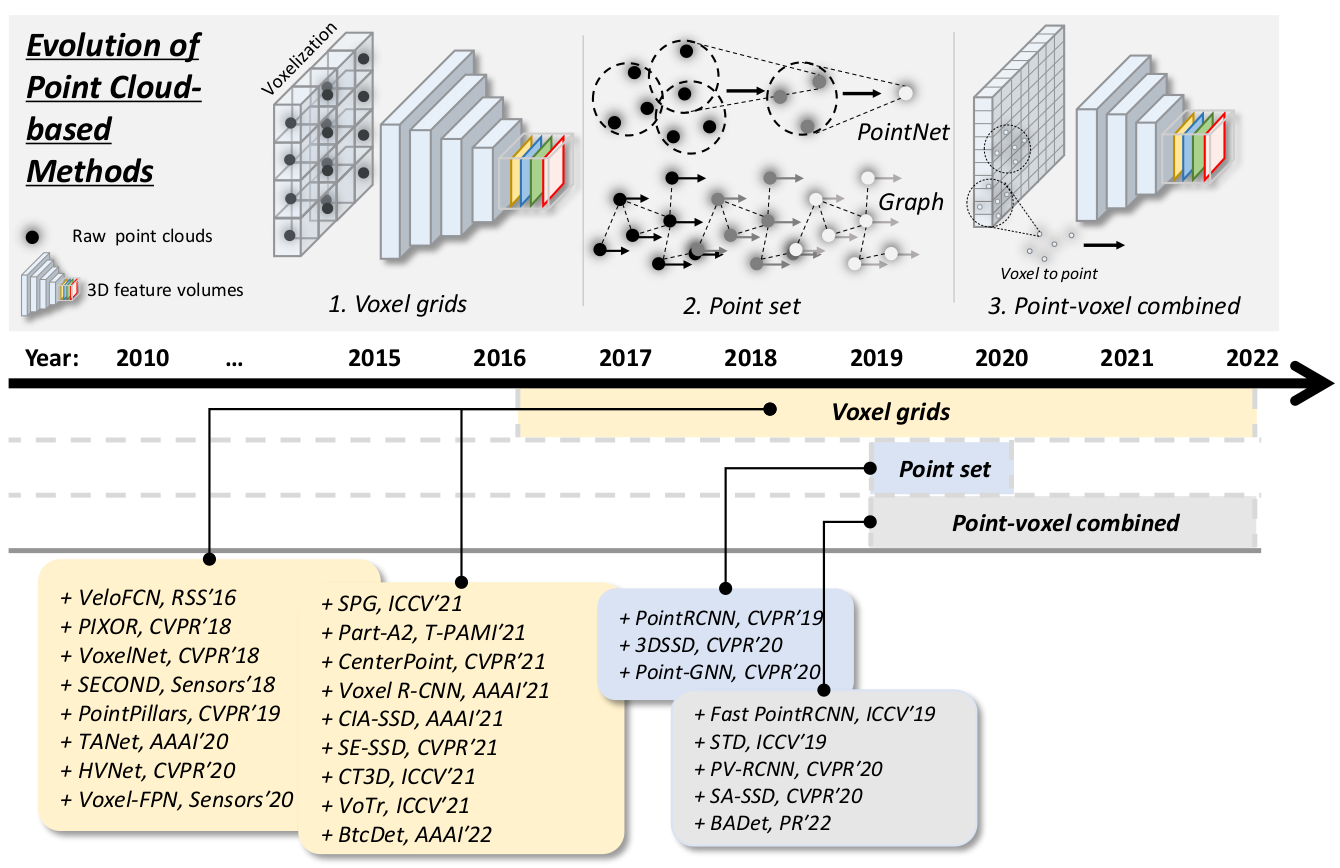
\includegraphics[width=1\linewidth]{figures/evolution_point_cloud_based.png}
    \caption{سیر زمانی پیشرفت روش‌های مبتنی بر ابر نقاط \cite{qian20223d}}
    \label{fig:evolution_point_cloude_based}
\end{figure}

\subsubsection{روش‌های تشخیص مبتنی بر واکسل}

این گروه از روش‌ها، ابر نقاط نامنظم را به شبکه‌های مرتب و فشرده دو بعدی و سه بعدی تبدیل می‌کنند. سپس آن‌ها را به شکل نمای دید پرنده\LTRfootnote{\lr{Bird's Eye View (BEV)}} دو بعدی تبدیل می‌کنند تا شبکه‌های پیچشی همانند تصاویر با آن برخورد کنند و توابع پیچش موثر و سریع‌تری داشته باشند. به عنوان مثال، مدل \lr{VoxelNet} ابر نقاط را به شبکه‌های واکسلی متراکم تقسیم‌بندی می‌کند و از شبکه‌های عصبی پیچشی سه بعدی برای پیچش در امتداد هر بعد استفاده می‌کند، اگرچه این رویکرد با هزینه محاسباتی و حافظه زیادی همراه است. از سوی دیگر، مدل \lr{SECOND} از عملیات پیچش پراکنده\LTRfootnote{\lr{Sparse Convolution}} استفاده می‌کند تا محاسبات غیرضروری ناشی از لایه‌گذاری صفر\LTRfootnote{\lr{Zero Padding}} در واکسل‌ها را کاهش دهد. مدلی معروف به نام \lr{PointPillars} واکسل‌ها را به شکل ستون‌های دربرگیرنده کل نقاط در راستای عمودی، در نمای دید پرنده امتداد می‌دهد. البته این روش به قیمت کاهش وضوح عمودی تمام می‌شود که بر کیفیت یادگیری بازنمایی تاثیر می‌گذارد، اما سرعت چشم‌گیری دارد \cite{qian20223d}.

برای مهار کردن این محدودیت \lr{PointPillars}، برخی از روش‌ها به شبکه‌های واکسلی باز‌گشتند. مدل \lr{Voxel R-CNN} ویژگی‌های واکسلی را با استفاده از پیچش‌های سه‌بعدی برای بهبود پیشنهاد\LTRfootnote{\lr{Proposal Refinement}}، جمع‌آوری می‌کند، در حالی که مدل \lr{SE-SSD} هم‌زمان یک شبکه عصبی دانش‌آموز را تحت راهنمایی دانش تصفیه‌شده شبکه عصبی استاد، نظارت می‌کند. روش‌های دیگر، استراتژی‌های چندمقیاسه واکسلیزه کردن را به جمع‌آوری ویژگی\LTRfootnote{\lr{Feature Extraction}} اضافه می‌کنند، از وابستگی‌های زمینه‌ای بین واکسل‌هایی با فواصل زیاد\LTRfootnote{\lr{Long Range Contextual Dependancies}} بهره‌می‌برند یا یادگیری شکل\LTRfootnote{\lr{Shape Learning}} را برای مقابله با مسائل مربوط به کیفیت ابر نقاط تحت تأثیر عواملی مانند شرایط جوی نامساعد، انسداد\LTRfootnote{\lr{Occlusion}} و انتهای افق دید لایدار به کار می‌گیرند. لازم به ذکر است که روش‌های مبتنی بر شبکه‌های واکسلی، از بازنمایی نمای دید پرنده مرتبط بهره‌می‌برند که ابهام در مقیاس را کاهش می‌دهد و حداقل انسدادها را دارد \cite{qian20223d}.

\subsubsection{روش‌های تشخیص مبتنی بر نقطه}
این دسته از روش‌ها از عامل‌هایی استفاده می‌کنند که وابسته به ترتیب نیستند و در نتیجه امکان شناسایی ساختارهای محلی و الگوهای پیچیده در ابر نقاط را بدون نیاز به کوانتش\LTRfootnote{\lr{Quantization}} ممکن می‌سازند. این رویکرد، خصوصیات هندسی و ذاتی ابر نقاط خام را حفظ می‌کند. به عنوان مثال، مدل \lr{PointRCNN} از یک تکنیک مشابه مدل معروف \lr{PointNet} برای یادگیری نشانه‌های معنادار\LTRfootnote{\lr{Semantic Cues}} نقاط گوشه‌ای جسم تشخیص داده شده استفاده می‌کند، که امکان تولید پیشنهادات سه‌بعدی\LTRfootnote{\lr{3D Proposals}} برای شکل جسم را به صورت گام‌به‌گام ممکن می‌سازد. لازم به ذکر است که روش‌های مجموعه‌ی \lr{PointNet}، به طور گسترده‌ای از ابزارهای نمونه‌افزایی\LTRfootnote{\lr{Upsampling}} و پخش اطلاعات مفهومی در نقاط کلیدی بهره می‌برند.

از طرف دیگر، رویکرد مدل \lr{3DSSD} برای افزایش بهره‌وری سیاست نمونه‌برداری نقاط، نگرشی تازه به فاصله ویژگی‌های\LTRfootnote{Feature Distance} نقاط به همراه فاصله اقلیدسی\LTRfootnote{Euclidean Distance} آن‌ها می‌اندازد. مدل \lr{Point-GNN} با الهام گرفتن از عملکرد موفق ابر نقاط در وظایفی مانند طبقه‌بندی\LTRfootnote{Classification} و بخش‌بندی معنایی\LTRfootnote{Semantic Segmentation}، تصمیم‌گیری را بر اساس گراف‌های همسایه محلی نقاط ساخته شده‌اند، انجام می‌دهد. در این گراف‌ها، هر گره به صورت تدریجی اطلاعات مفهومی را از نواحی مجاور خود جمع‌آوری می‌کند. با این حال، لازم به ذکر است که روش‌های مبتنی بر نقاط، ممکن است مصرف محاسباتی بسیار بالایی داشته باشند و با پیچیدگی جستجوی توپی\LTRfootnote{‌Ball Query Complexity} \lr{O(k$\cdot$|$\chi$|)} مواجه باشند. برخی رویکردها این چالش را با پیاده‌سازی گروه‌بندی چند مقیاسی و چند رزولوشنی حل می‌کنند؛ اما این روش با افزایش تعداد نقاط در مجموعه \lr{$\chi$}، سربار پردازشی خواهد داشت \cite{qian20223d}.

\subsubsection{روش‌های تشخیص مبتنی بر واکسل-نقطه}

روش‌های موجود در این دسته، یک رویکرد نوآورانه معرفی می‌کنند که نقاط قوت دو روش قبلی را ترکیب می‌کند. روش‌های مبتنی بر واکسل از لحاظ محاسباتی کارآمد هستند، اما ممکن است الگوهای ریز همانند انسان‌ها را نادیده بگیرند و بر روی بهبود دقت در هر تکرار\LTRfootnote{\lr{Iteration}} یادگیری، تاثیر منفی بگذارند. متقابلا، روش‌های مبتنی بر نقاط معمولاً تاخیر نسبی بیشتری دارند اما در حفظ ناهنجاری و محلی بودن ابر نقاط بهتر عمل می‌کنند. به عنوان مثال، مدل \lr{STD} از \lr{PointNet++} برای متراکم‌سازی اطلاعات معنادار بین نقاط پراکنده استفاده می‌کند، سپس آنها را واکسلیزه  می‌‌کند و یک بازنمایی متراکم‌تر برای بهبود دقت ایجاد می‌کند.  مدل \lr{PV-RCNN}، با یکپارچه‌کردن بهره‌وری اطلاعات مفید با استفاده از عملیات پیچش پراکنده سه‌بعدی\LTRfootnote{\lr{3D Sparse Convolutions}}، و استخراج داده‌های حائز اهمیت و معنادار با استفاده از مجموعه‌های شبه  \lr{PointNet}، فرآیند یادگیری معانی متمایزتر را تقویت می‌کند. مدل \lr{SA-SSD}، با استفاده از یک شبکه عصبی کمکی، ویژگی‌های واکسل‌هایی که با استفاده از پیچش پراکنده سه‌بعدی بدست آمده است را نسبت به ساختار نقاط خود آگاه‌تر می‌کند. یعنی این شبکه عصبی کمکی، ساختار اشکال داخل واکسل‌ها را حدس می‌زند و سعی می‌کند اشکالی که نقاط آنها ناقص هستند را تکمیل کند \cite{qian20223d}.

\subsubsection{تشخیص اجسام سه‌بعدی در دوقلوهای دیجیتال}

در حال حاضر، به نظر می‌آید که روش‌های مبتنی بر واکسل انتخاب اصلی محققین هستند، همانطور که در \cref{fig:evolution_point_cloude_based} نیز مشاهده می‌شود. روش‌های مبتنی بر واکسل، قابلیت انعطاف بالا برای پیاده‌سازی در سخت‌افزار را دارند و دقتی قابل توجه و زمان پاسخ نسبتاً کمتری دارند. از سوی دیگر، روش‌های مبتنی بر نقطه توانایی حفظ ویژگی‌های محلی فضایی\LTRfootnote{\lr{Spatially-Local Features}} ابرنقاط را دارند، اما نسبت به روش‌های مبتنی بر واکسل زمان بیشتری برای پیشروی رو به جلو\LTRfootnote{\lr{Feedforward}} دارند. با مقایسه سه روش تشخیص مبتنی بر ابر نقاط، آشکار می‌شود که روش‌های مبتنی بر واکسل، همچنان به عنوان جهتی بسیار امیدبخش‌تر در کاربردهای بلادرنگ، به عنوان مثال در حوزه رانندگی خودروهای خودران و دوقلوهای دیجیتال، مورد مطالعه قرار گرفته شده‌اند.

\subsection{مجموعه داده مدل‌های تشخیص سه‌بعدی}

دسترسی به مجموعه‌ داده‌هایی\LTRfootnote{\lr{Datasets}} با مقیاس‌های عظیم، نقش مهمی در پیشرفت حوزه‌های مختلف هوش‌ مصنوعی ایفا کرده است. در زمینه تشخیص اجسام سه‌بعدی، چندین مجموعه داده عمومی به تحقیقات کمک کرده‌اند. مجموعه‌ داده‌های معروفی از جمله \lr{KITTI} \cite{geiger2012we}، \lr{nuScenes} \cite{caesar2020nuscenes}، و \lr{Waymo Open} \cite{sun2020scalability}   وجود دارند که به عنوان  منابع گسترده برای کاربردهای مرتبط با خودرو‌های خودران به کار می‌روند. این مجموعه‌ داده‌ها در ابعاد مختلف از جمله اندازه\LTRfootnote{\lr{Size}}، تنوع\LTRfootnote{\lr{Diversity}}، مزایا و معایب با یکدیگر تفاوت دارند.

\subsubsection{اندازه}

مجموعه داده \lr{KITTI} شامل 200,000 کادر محصورکننده حاشیه‌نویسی شده\LTRfootnote{\lr{Annotated Bounding Boxes}} و توزیع شده در 15,000 فریم می‌شود. این مجموعه داده برای آموزش و آزمون، نمونه‌هایی تقریباً مشابه دارد. در مقابل، مجموعه داده \lr{nuScenes} شامل 1.4 میلیون کادر محصورکننده توزیع شده در 40,000 فریم است و مجموعه‌هایی جدا و متمایز برای آموزش، اعتبارسنجی و آزمون دارد. مجموعه داده \lr{Waymo Open} با بیش از 112 میلیون کادر محصورکننده در 200,000 فریم و داده‌هایی با مقیاس بزرگ برای آموزش، اعتبارسنجی و آزمون، از سایرین برجسته‌تر است. لازم به ذکر است که در حالی که حاشیه‌نویسی‌ها برای آموزش و اعتبارسنجی در دسترس هستند، هیچ یک از این مجموعه‌های داده حاشیه‌نویسی‌ای برای مجموعه‌ آزمون ارائه نمی‌دهند و شرکت‌کنندگان باید پیش‌بینی‌های خود را در وبسایت آنلاین مجموعه‌ داده‌ها  ارسال کرده و ارزیابی\LTRfootnote{\lr{Benchmark}} کنند \cite{qian20223d}.

\subsubsection{تنوع}

مجموعه داده \lr{KITTI}، داده‌ها را از 50 صحنه ترافیکی مختلف با 8 کلاس اجسام فراهم می‌کند و ارزیابی آنلاین آن بر روی کلاس‌های خودرو، پیاده‌رو و دوچرخه‌سوار تمرکز دارد. این مجموعه داده صحنه‌ها را بر اساس میزان ارتفاع کادر‌های محصور کننده دوبعدی، میزان انسداد در ابرنقاط و میزان برش ابرنقاط به علت رسیدن به انتهای افق دید لایدار، طبقه‌بندی می‌کند. از طرفی، مجموعه داده \lr{nuScenes} از 1,000 صحنه ترافیکی در 23 کلاس داده ارائه می‌دهد و در ارزیابی آنلاین، تمرکز خود را بر روی 10 کلاس تشخیص اجسام سه‌بعدی می‌گذارد. مجموعه داده \lr{Waymo Open} شامل 1,150 صحنه ترافیکی در 4 کلاس است و ارزیابی آنلاین آن بر روی سه کلاس مشابه با \lr{KITTI} تمرکز دارد. لازم به ذکر است که مجموعه داده‌های \lr{nuScenes} و \lr{Waymo Open}، داده‌های خود را در شرایط جوی و روشنایی مختلف شامل باران، مه، برف، روز و شب جمع‌آوری کرده‌اند و تنوع بیشتری در سناریوها نسبت به \lr{KITTI} ارائه می‌دهند، که تنها به روزهای آفتابی محدود است \cite{qian20223d}.

\begin{table}[h!]
    \centering
    \caption{توزیع داده در داده‌های آموزش \lr{KITTI}. کلاس خودرو \% 99.82 سه کلاس اصلی (خودرو، عابرپیاده، دوچرخه‌سوار) را تشکیل می‌دهد \cite{qian20223d}.}
    \begin{tabular}{ccccccccc}
         \hline
         کلاس & انسان نشسته & قطار & غیره & کامیون & دوچرخه‌سوار & ون & عابر‌پیاده & خودرو  \\
         \hline
          تعداد & 56 & 224 & 337 & 448 & 734 & 1297 & 2,207 & 14,357 \\
         \hline
    \end{tabular}
    \label{tab:KITTI_class_table}
\end{table}

\begin{table}[h!]
    \centering
    \caption{توزیع داده در داده‌های آموزش \lr{nuScenes} \cite{qian20223d}.}
    \label{tab:nuSceness_class_table}
    \begin{tabular}{ccccccccc}
         \hline
         کلاس & اتوبوس & تریلی & کامیون & مخروط ترافیکی & مانع ترافیکی & عابر پیاده & خودرو\\
         \hline
         تعداد & 13,163 & 20,701 & 72,815 & 82,362 & 125,095 & 185,847 & 413,318 \\
         \hline
    \end{tabular}
    
    \begin{tabular}{cccc}
        \\
        \hline
        کلاس‌ & دوچرخه & موتورسیکلت & جرثقیل \\
        \hline
         تعداد & 9,478 & 10,109 & 11,993 \\
        \hline
    \end{tabular}
\end{table}

\subsubsection{مزایا و معایب}

این مجموعه‌ داده‌ها تاثیر قابل توجهی بر جامعه علمی داشته‌اند. به ویژه \lr{KITTI} تأثیر عمیقی در زمینه‌های جمع‌آوری داده‌ها، پروتکل‌ها و ارزیابی‌ داشته است. با این حال، بایستی توجه داشت که جمع‌آوری داده‌های \lr{KITTI}، تنها در روزهای آفتابی انجام شده است. یعنی شرایط روشنایی و جوی که می‌تواند تأثیر زیادی بر سناریوهای واقعی داشته باشد، در نظر گرفته نشده است. این مشکل توسط مجموعه داده‌های \lr{nuScenes} و \lr{Waymo Open} حل شده است. این دو مجموعه‌ داده، داده‌های خود را در شرایط مختلف جوی و روشنایی مانند باران، مه، برف، روز و شب جمع‌آوری می‌کنند. علاوه بر این، مجموعه‌ داده‌های واقعی معمولاً از عدم توازن کلاس‌ها\LTRfootnote{\lr{Data Imbalance}} رنج می‌برند، که اکثر کلاس‌های آنها به درصد کوچکی از دسته‌ها تعلق دارند. با توجه به \cref{tab:KITTI_class_table} و \cref{tab:nuSceness_class_table}، می‌توان این مشکل را در مجموعه‌ داده‌های \lr{nuScenes} و \lr{KITTI} مشاهده کرد \cite{qian20223d}. 

\subsection{معیارهای ارزیابی}

در بخش قبلی مشاهده کردیم که مجموعه دادگانی وجود دارند که برای آموزش، آزمون و ارزیابی مدل‌های تشخیص اجسام سه‌بعدی،‌ طراحی شده‌اند. حال به روش‌هایی که این مجموعه‌دادگان با استفاده از آن مدل را ارزیابی می‌کنند، می‌پردازیم. در ابتدا لازم است که مفاهیمی را توضیح دهیم:

\subsubsection{ماتریس درهم‌ ریختگی}

 ماتریس درهم‌ ریختگی\LTRfootnote{\lr{Confusion Matrix}}، ابزاری حیاتی در یادگیری ماشین و آمار است. \begin{figure}[h!]
    \centering
    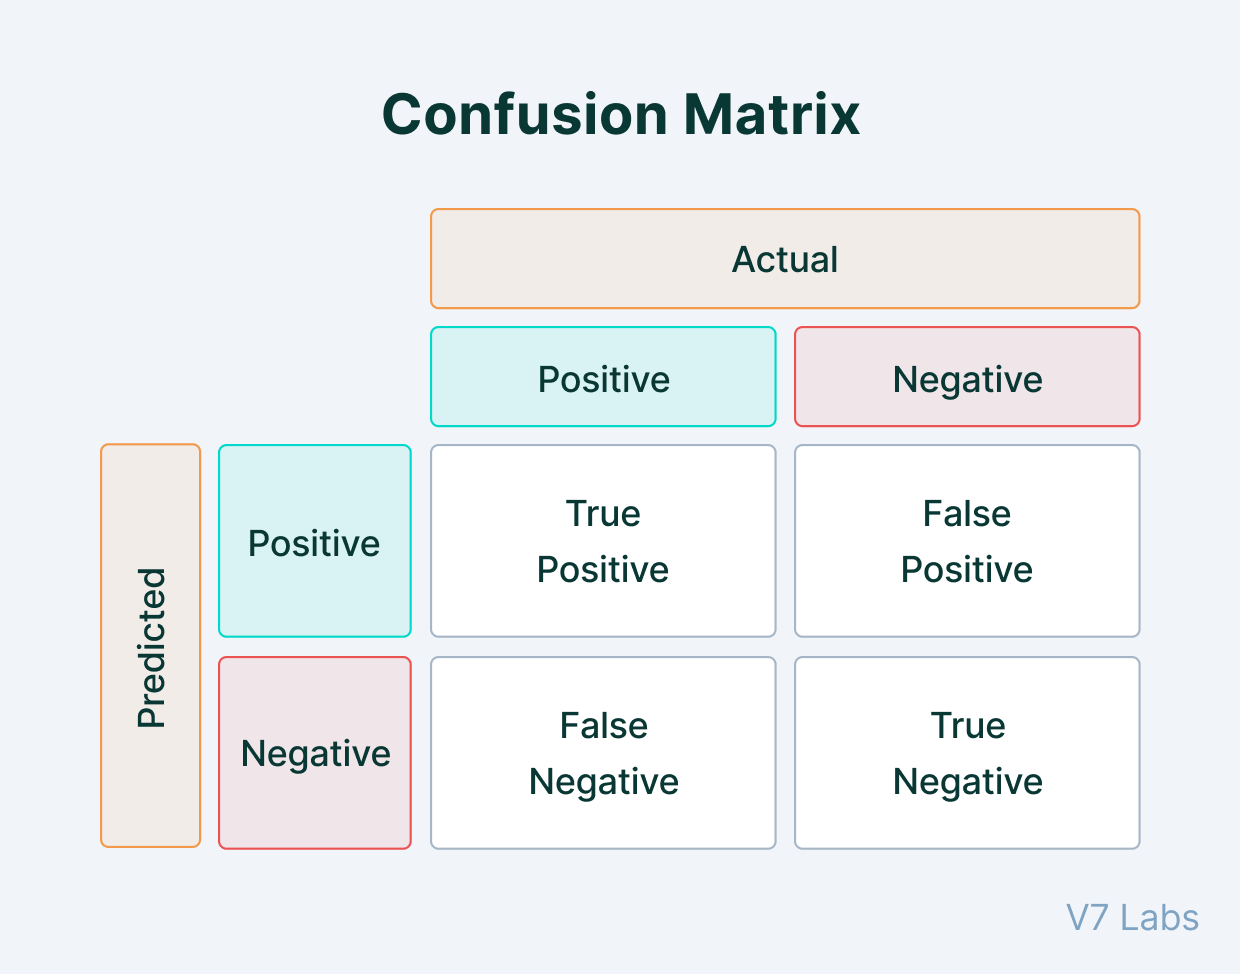
\includegraphics[width=0.75\linewidth]{figures/Confusion_Matrix.png}
    \caption{ماتریس در هم‌ ریختگی \cite{V7:mAP_Explanation}}
    \label{fig:confusion_matrix}
\end{figure}این ماتریس، خلاصه‌ای از مقایسه‌ پیش‌بینی‌های مدل با مقادیر واقعی\LTRfootnote{\lr{Ground Truth}} ارائه می‌دهد. این ماتریس از چهار بخش تشکیل شده است:
 \begin{enumerate}
     \item مثبت‌های واقعی\LTRfootnote{\lr{True Positive (TP)}} (نمونه‌های مثبتی که به درستی تشخیص داده شده‌اند)
     \item منفی‌های واقعی\LTRfootnote{\lr{True Negative (TN)}} (نمونه‌های منفی که درستی تشخیص داده شده‌اند)
     \item مثبت‌های کاذب\LTRfootnote{\lr{False Positives (FP)}} (نمونه‌های منفی‌ که به اشتباه به عنوان مثبت تشخیص داده شده‌اند)
     \item منفی‌های کاذب\LTRfootnote{\lr{False Negatives (FN)}} (نمونه‌های مثبت که به اشتباه به عنوان منفی تشخیص داده شده‌اند)
 \end{enumerate}

\subsubsection{دقت}
دقت\LTRfootnote{\lr{Precision}}، نشان‌دهنده این است که چه تعداد از نمونه‌هایی که مثبت پیش‌بینی شده‌اند، درست پیش‌بینی شده‌اند و رابطه‌ی آن از روش زیر قابل محاسبه است:
\begin{equation}
    Precision = \dfrac{TP}{TP+FP}
\end{equation}

\subsubsection{پوشش}
پوشش\LTRfootnote{\lr{Recall}}، مشخص می‌کند که چه تعداد از نمونه‌هایی که مثبت بوده‌اند، درست پیش‌بینی شده‌اند. رابطه‌ی آن به شکل زیر نوشته می‌شود:
\begin{equation}
    Recall = \dfrac{TP}{TP+FN}
\end{equation}

\subsubsection{نسبت اشتراک بر روی اجتماع}
معیار نسبت اشتراک بر روی اجتماع\LTRfootnote{\lr{Intersection over Union (IoU)}}، نشان‌دهنده انطباق مختصات کادر محصورکننده تخمین زده شده با کادر واقعی (یا داده‌های واقعی) است.

\begin{figure}[h!]
    \centering
    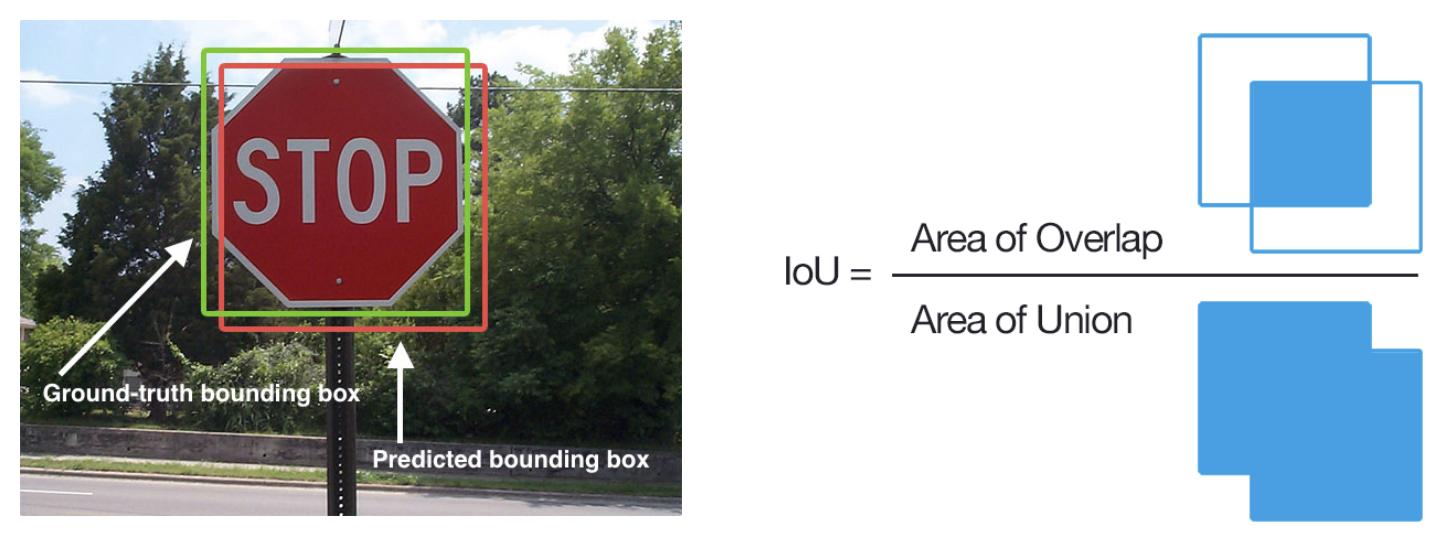
\includegraphics[width=0.8\linewidth]{figures/IoU.png}
    \caption{نسبت اشتراک بر روی اجتماع \cite{V7:mAP_Explanation}}
    \label{fig:IoU}
\end{figure}

همانطور که در \cref{fig:IoU} مشاهده می‌کنیم، نحوه محاسبه معیار نسبت اشتراک بر روی اجتماع نشان داده شده است. هدف از این کار، سنجیدن واقعی یا کاذب بودن تشخیص مدل است.

برای سنجش واقعی یا کاذب بودن، عموما حد آستانه‌ای\LTRfootnote{\lr{Threshold}} را برای نسبت اشتراک بر روی اجتماع می‌گذارند. به طور مثال در \cref{fig:IoU_FP_TP}، حد آستانه برابر با ۵.۰ است. پس کادر تخمینی‌ای که نسبت اشتراک بر روی اجتماع آن کمتر از این مقدار باشد، مثبت کاذب است و اگر بیشتر از حد آستانه باشد، مثبت واقعی است.

\begin{figure}[h!]
    \centering
    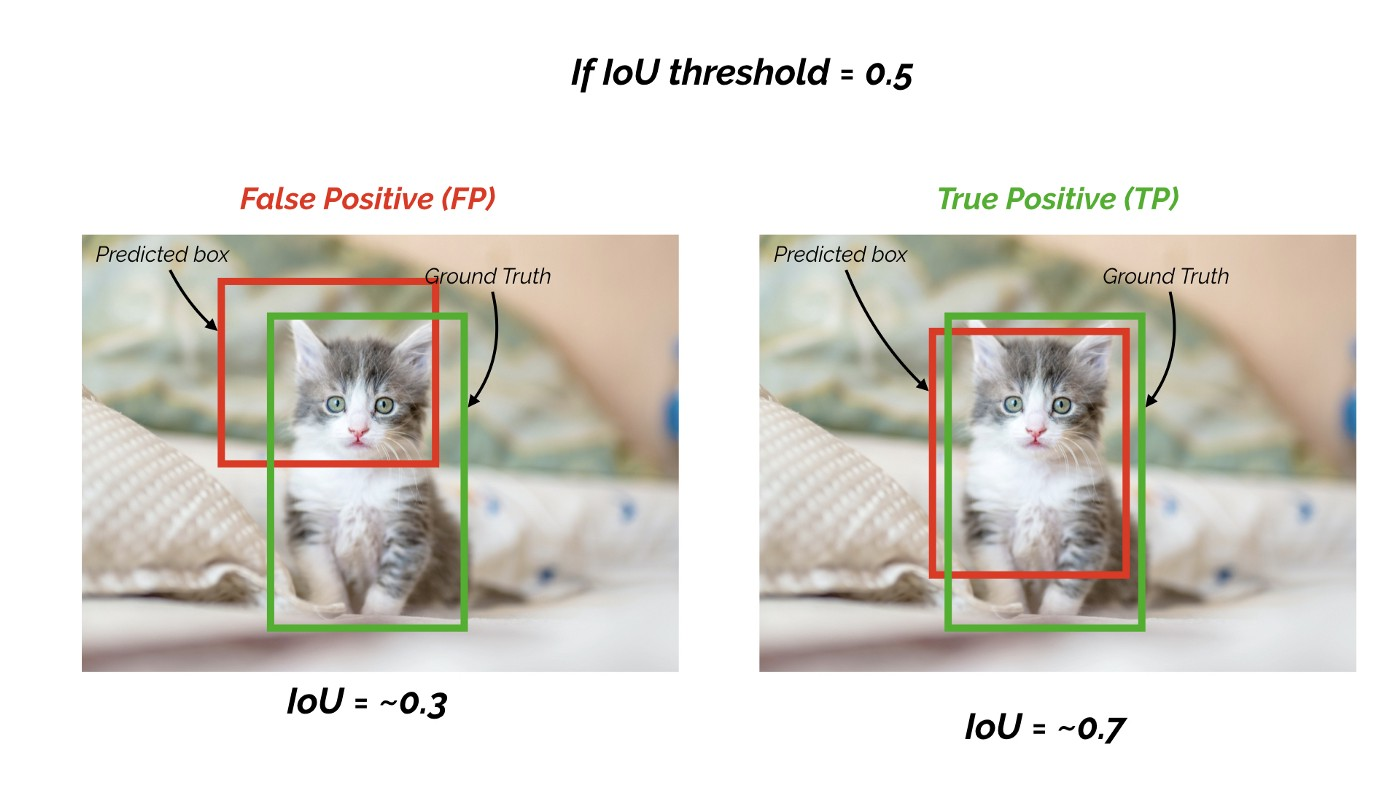
\includegraphics[width=0.8\linewidth]{figures/IoU_FP_TP.png}
    \caption{سنجش واقعی یا کاذب بودن براساس حد آستانه \cite{V7:mAP_Explanation}}
    \label{fig:IoU_FP_TP}
\end{figure}

\begin{figure}[h!]
    \centering
    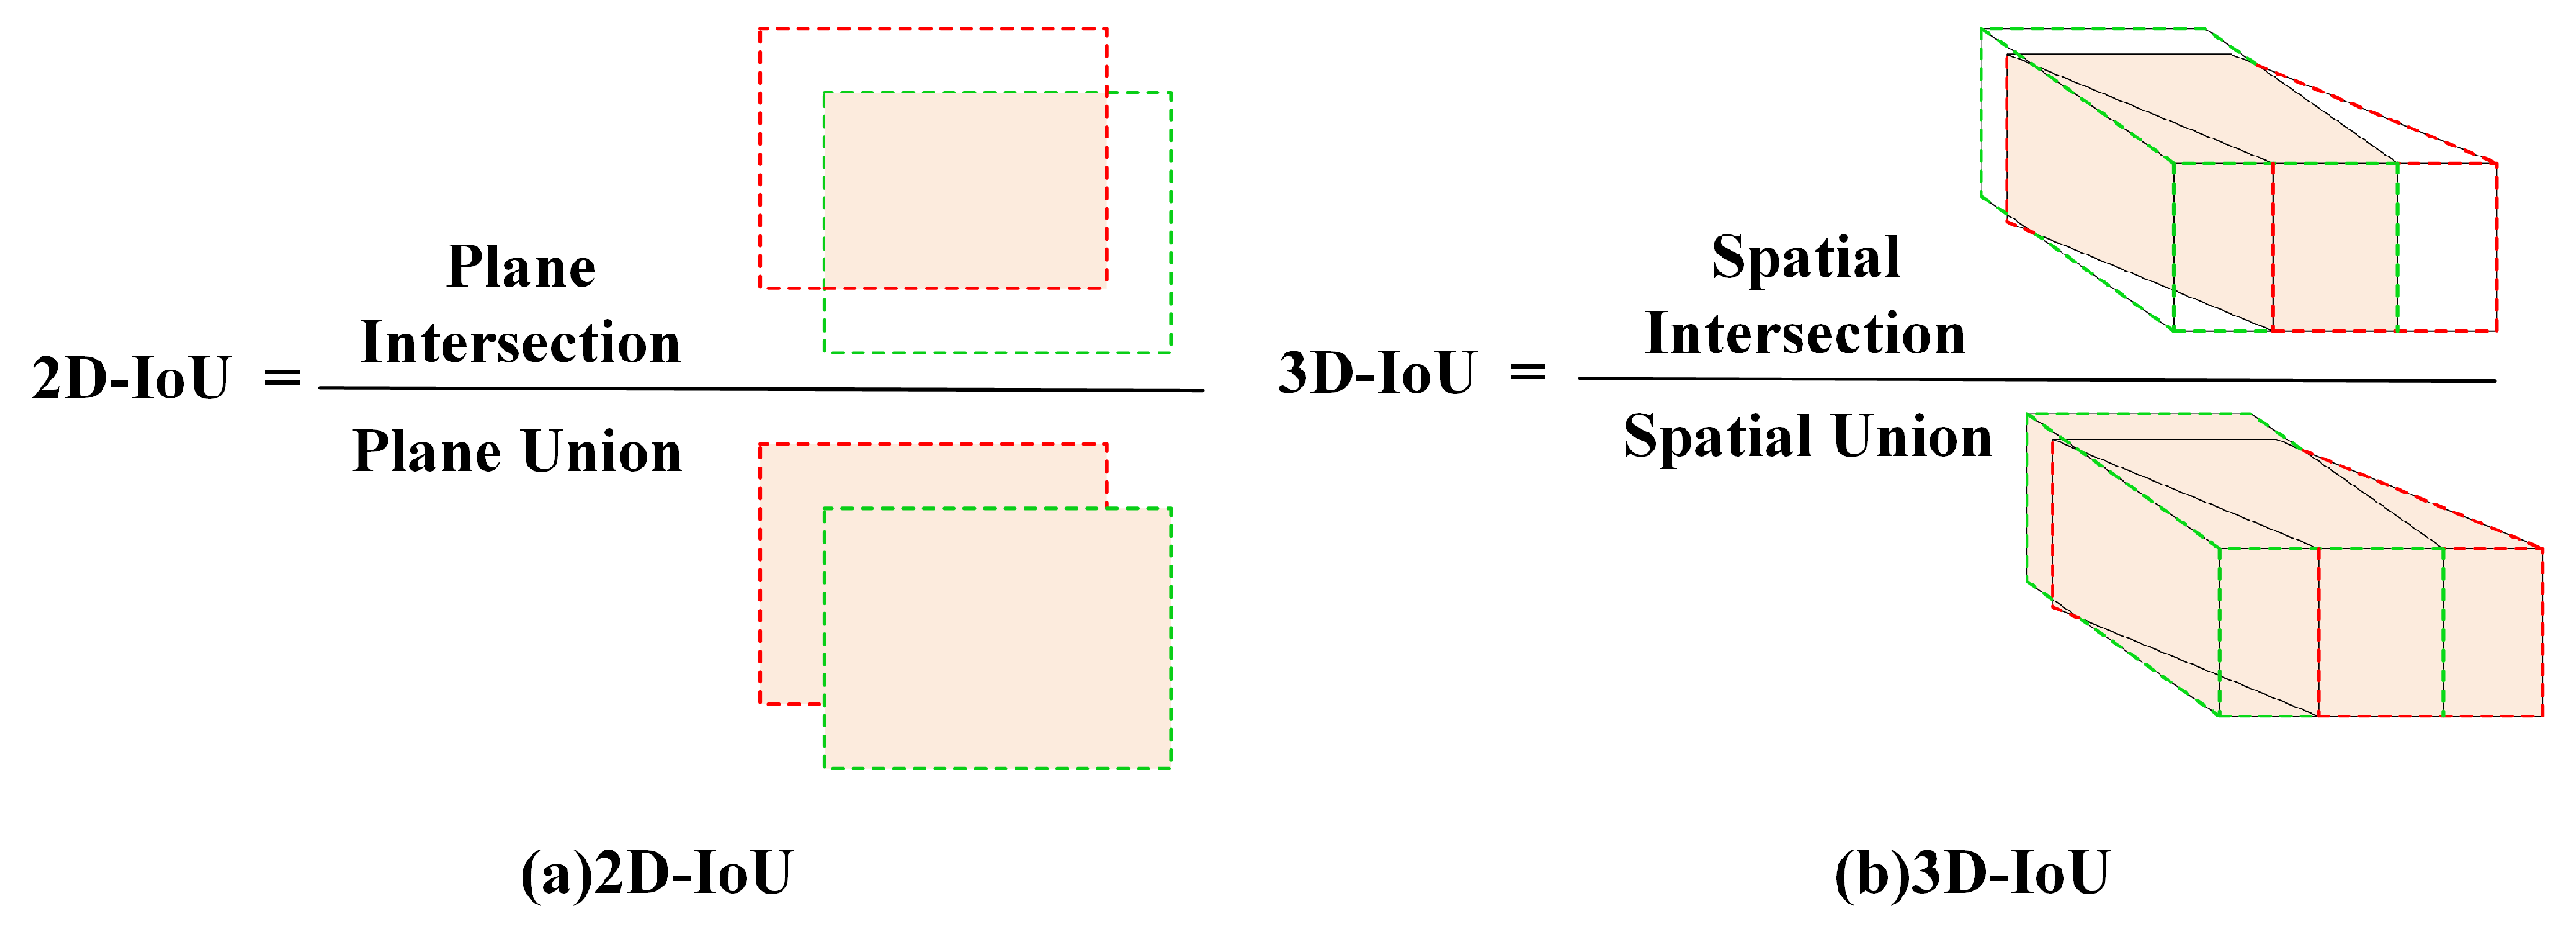
\includegraphics[width=0.8\linewidth]{figures/3d_IoU.png}
    \caption{نسبت اشتراک بر روی اجتماع در فضای سه‌بعدی و  دو بعدی \cite{han2022hybrid}}
    \label{fig:3d_IoU}
\end{figure}

این معیار فقط برای تصاویر دوبعدی نیست و در تشخیص اجسام سه‌بعدی نیز استفاده می‌شود. اما محاسبات این نسبت در اشکال سه‌بعدی بسیار دشوارتر است و عموما از تخمین برای محاسبه حجم مشترک استفاده می‌شود\LTRfootnote{\url{https://pytorch3d.org/docs/iou3d}}.


\subsubsection{میانگین دقت و میانگین دقت درون‌یابی شده}

در تشخیص اجسام سه‌بعدی و دوبعدی، امتیاز اطمینان\LTRfootnote{\lr{Confidence Score}} برای هر کادر محصورکننده تخمین زده شده محاسبه می‌شود. فرض کنیم زیرمجموعه نزولی پیش‌بینی‌‌ $\{y_1, \ldots, y_n\}$ وجود دارد که به ترتیب امتیاز اطمینان $s_i$ مرتب شده است؛ پیش‌بینی $y_i$ مثبت واقعی است اگر نسبت اشتراک بر روی اجتماع کادر محصورکننده $\beta_i$، از حد آستانه مشخص شده بیشتر باشد. اگر خلاف این باشد، مثبت کاذب است \cite{qian20223d}. نمودار زیگ-زاگی دقت-پوشش این زیرمجموعه، به راحتی قابل رسم است و مقدار میانگین دقت\LTRfootnote{\lr{Average Precision (AP)}} آن برابر با مساحت زیر نمودار است. اما در عمل، محاسبه‌ی مساحت زیر نمودار دشوار است. به همین دلیل محققانی در مسابقه \lr{PASCAL VOC}، روش‌هایی برای تسهیل محسابه میانگین دقت کشف کردند که از میانگین دقت درون‌یابی شده\LTRfootnote{\lr{Interpolated AP}} استفاده می‌کند.

برای درک بهتر محاسبه میانگین دقت درون‌یابی شده، مثالی آورده شده است. فرض کنیم تشخیص‌‌ دهنده اجسام، خروجی زیر را داده است و آن را براساس امتیاز اطمینان هر تصویر، مرتب کرده‌ است.

\begin{figure}[h!]
    \centering
    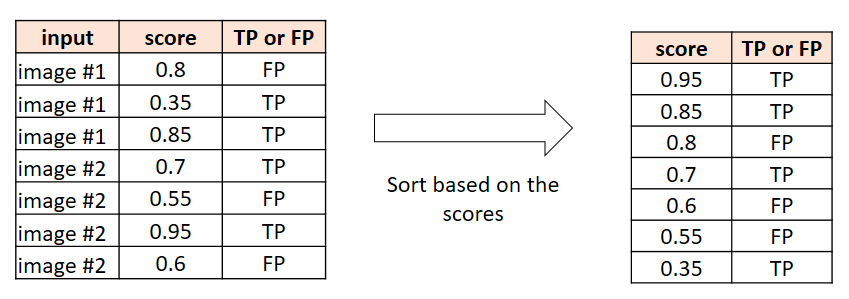
\includegraphics[width=1\linewidth]{figures/bbox_sorting.png}
    \caption{مرتب‌ سازی براساس امتیاز اطمینان کادرهای پیش‌بینی شده}
    \label{fig:bbox_sorting}
\end{figure}
حال مقادیر دقت و پوشش هر تخمین را به صورت تجمعی\LTRfootnote{\lr{Accumulated}} محاسبه می‌کنیم:

\begin{figure}[h!]
    \centering
    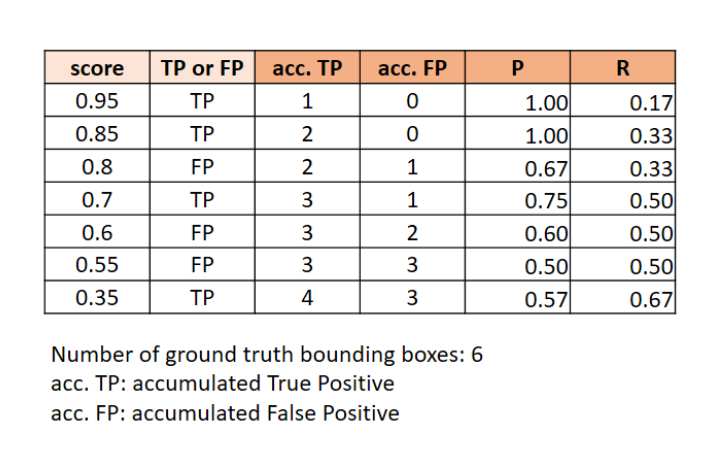
\includegraphics[width=0.75\linewidth]{figures/precision_recall_calculation.png}
    \caption{جدول محاسبه دقت و پوشش هر تخمین به صورت تجمعی}
    \label{fig:precision_recall_calculation}
\end{figure}

فرمول محاسبه پوشش و دقت به شکل زیر تعریف می‌شود:
\begin{equation}
    P = \dfrac{acc.TP}{acc.TP + acc.FP}\\
    R = \dfrac{acc.TP}{N}
    \label{P_R}
\end{equation}
که \lr{N} تعداد کادر محصورکننده‌های واقعی\LTRfootnote{\lr{Ground-Truth Bounding Boxes}} است. \cref{fig:precision_recall_calculation} جدول پوشش و دقت را نشان می‌دهد که با استفاده از \cref{P_R} محاسبه شده‌اند.
\\
\\
حال نمودار دقت-پوشش را رسم می‌کنیم. مشاهده می‌کنیم که نمودار به شکل زیگ-زاگی در آمده است. این اتفاق به علت مرتب‌سازی جدول براساس امتیاز اطمینان رخ داده است.

\begin{figure}[h!]
    \centering
    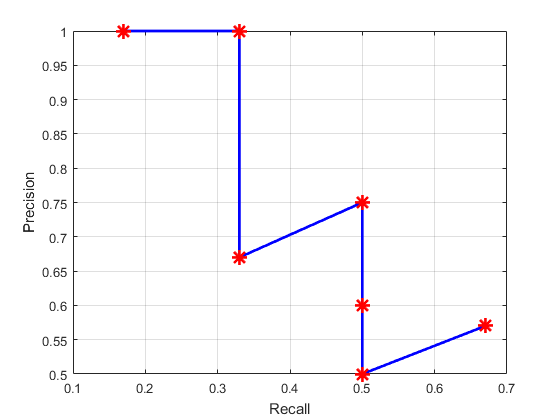
\includegraphics[width=0.8\linewidth]{figures/precision-recall_plot.png}
    \caption{نمودار دقت-پوشش}
    \label{fig:enter-label}
\end{figure}

برگزارکنندگان مسابقه \lr{PASCAL VOC} به دنبال راهی بودند که مساحت زیر نمودار دقت-پوشش را بتوان محاسبه کرد. از این رو به روش درون‌یابی میانگین دقت روی آوردند. 
\begin{definition}
    معیار پوشش درون‌یابی شده $AP \vert_{R_N}$، در زیرمجموعه پوشش $R$ محاسبه شده است که از $N$  سطح پوشش به شکل زیر تشکیل شده است \cite{qian20223d}: 
    \begin{equation}
        AP\vert_{R_N} = \frac{1}{N}\sum_{r\in{R}}{P_{interpolate}(r)}
        \label{AP_interpolate}
    \end{equation}
    که $R = \left[r_0, r_0 + \frac{r_1 - r_0}{N - 1}, r_0 + \frac{2(r_1 - r_0)}{N - 1}, \ldots, r_1\right]$. به ازای هر سطح پوشش $r$، دقت متناظر آن با بیشینه سطح پوشش‌های بیشتر یا مساوی $r$ درون‌یابی می‌شود، یا به عبارتی
    \begin{equation}
        P_{interpolate}(r) = \max_{\Tilde{r}:\Tilde{r}\ge r}{P(\Tilde{r})}
    \end{equation}
\end{definition}
حاصل درون‌یابی مثال زده شده، نمودار زیر است:
\begin{figure}[h!]
    \centering
    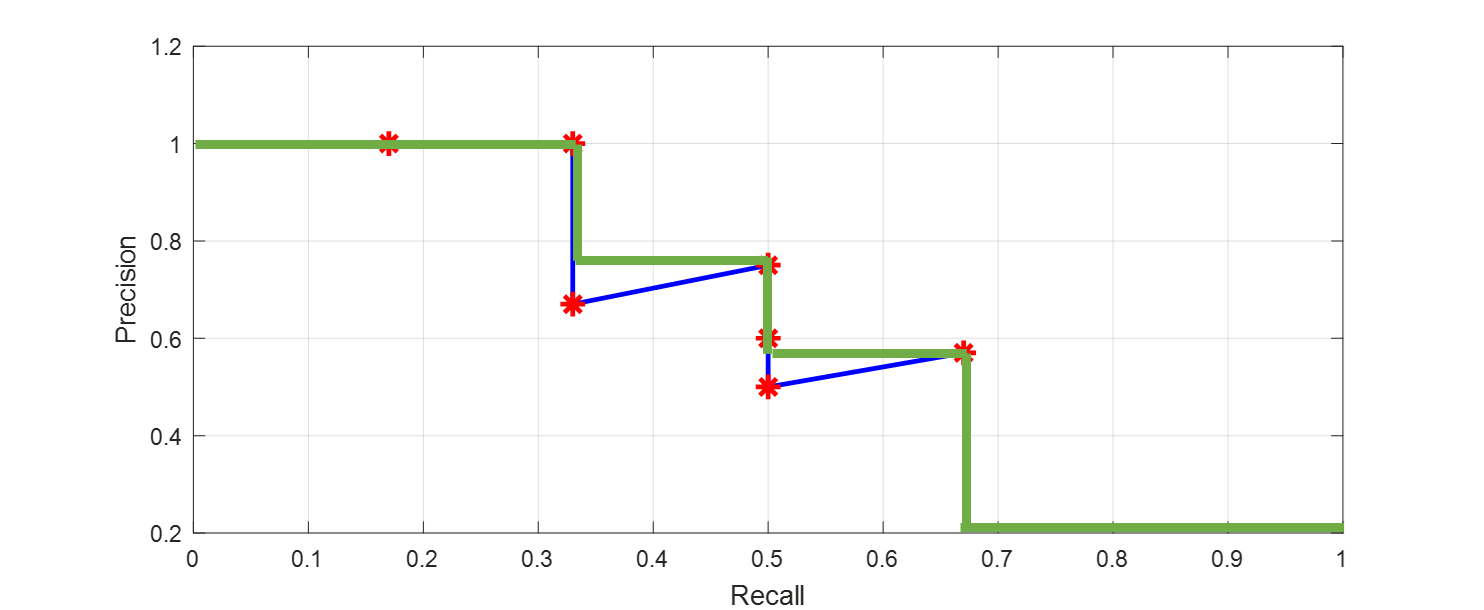
\includegraphics[width=1\linewidth]{figures/precision_recall_interpolate.png}
    \caption{نمودار دقت-پوشش درون‌یابی شده}
    \label{fig:precision-recall_interpolate}
\end{figure}

حال با فرض اینکه ۱۱ سطح پوشش داریم (طبق قرارداد \lr{PASCAL VOC} که البته در حال حاضر به ۴۰ سطح رسیده است)، میانگین دقت را طبق \cref{AP_interpolate}
 محاسبه می‌کنیم که خواهیم داشت:
 \begin{equation}
    AP = \frac{1}{11}(P_{interp}(0) + P_{interp}(0.1) + \ldots + P_{interp}(0.9) + P_{interp}(1))
 \end{equation}
 
\subsubsection{معیار \lr{mAP}}

معیار \lr{mAP}، عموما برای ارزیابی مدل‌های تشخیص اجسام در تصاویر دوبعدی (مانند \lr{Fast R-CNN}، \lr{YOLO}، \lr{Mask R-CNN} و غیره) استفاده می‌شود. این مقدار با میانگین گرفتن از میانگین دقت\LTRfootnote{\lr{Average Precision}} کلاس‌ها محاسبه می‌شود و مقداری بین ۰ تا ۱ دارد.

فرمول محاسبه‌ $mAP$ به شکل زیر است:
\begin{equation}
    mAP = \frac{1}{K}\sum_{C_i \in C}{AP_{Cـi}}
\end{equation}
 که $AP$ همان میانگین دقت است، $C$ مجموعه کلاس‌ها است و $K$ تعداد کلاس‌ها است. مقدار میانگین دقت می‌تواند به طور عادی با بدست آوردن سطح زیر نمودار محاسبه شود یا از حالت درون‌یابی شده آن یا $AP_{interpolate}$ استفاده شود. عموما از حالت دوم استفاده می‌شود زیرا نسبت به تغییرات پوشش حساس نیست و نتیجه بهتری می‌دهد.

 \subsubsection{معیار ارزیابی \lr{KITTI}}
مجموعه داده \lr{KITTI}، از میانگین دقت درون‌یابی شده و استاندارد $AP \vert_{R_{11}}$، به عنوان معیار اصلی ارزیابی تشخیص دهنده $\mathcal{F} (\mathcal{X} ; \theta)$ استفاده می‌کند. مجموعه داده \lr{KITTI}، عموما از دو جدول رده‌بندی برای سنجش مدل‌ها استفاده می‌کند:
\begin{enumerate}
    \item تشخیص سه‌بعدی
    \item  تشخیص از نمای دید پرنده \lr{(BEV)}
\end{enumerate}
تشخیص سه‌بعدی، مقدار میانگین دقت درون‌یابی شده‌ $AP_{3D} \vert_{R_{11}}$ را با آستانه‌های ۷.۰، ۵.۰ و ۵.۰ برای $IoU_{3D}$، به ترتیب در کلاس‌های خودرو، عابر پیاده و دوچرخه محاسبه می‌کند.
بیشتر سیاست‌های استفاده شده در تشخیص سه‌بعدی، در تشخیص از نمای دید پرنده نیز استفاده شده است؛ بجز محاسبه $IoU_{BEV}$، که با تصویر کردن کادر محصورکننده سه بعدی $\beta_{3D}$ از فضای سه‌بعدی به صفحه دو بعدی زمین، محاسبه می‌شود. توجه شود که مجموعه داده \lr{KITTI}، از سال ۲۰۱۹ به بعد سطوح پوشش خود را از ۱۱ سطح $\left[0, 1/10, 2/10, \ldots, 1\right]$ به ۴۰ سطح $\left[1/40, 2/40, 3/40, \ldots, 1\right]$ تغییر داده است. همانطور که دیده می‌شود، سطح پوشش در نسخه جدید، از صفر شروع نمی‌شود \cite{qian20223d}.

\subsubsection{معیار ارزیابی \lr{nuScenes}}

مجموعه داده \lr{nuScenes} از امتیاز \lr{NDS}\LTRfootnote{\lr{NuScenes Detection Score}}، به عنوان معیار اصلی خود برای ارزیابی تشخیص‌دهنده $\mathcal{F} (\mathcal{X} ; \theta)$ استفاده می‌کند. فرض کنیم زیرمجموعه‌ای از میانگین خطاها به نام $\varepsilon$ داریم، که متشکل از خطای تبدیل\LTRfootnote{\lr{Translation}}، ابعاد\LTRfootnote{\lr{Size}}، جهت‌گیری\LTRfootnote{\lr{Orientation}}، ویژگی\LTRfootnote{\lr{Attribute}} و سرعت\LTRfootnote{\lr{Velocity}} است. توجه شود که این خطاها مربوط به کادر محصورکننده تخمین زده شده توسط مدل است، که با کادر واقعی تفاوت‌هایی دارد. با نگارش زیرمجموعه فوق به صورت $\varepsilon = \{mATE, mASE, mAOE, mAAE, mAVE\}$، داریم: 
\begin{equation}
    NDS = \frac{1}{10}\left[5mAP + \sum_{err \in \varepsilon} (1 - \min(1, err)) \right]
\end{equation}

معیار \lr{NDS}، اشتراکی از میانگین وزن‌دار \lr{mAP} و  میانگین خطاهای مجموعه $\varepsilon$ در ۱۰ کلاس است. لازم به ذکر است که معیار \lr{mAP}، با استفاده از فاصله مرکز کادر تخمین زده شده و کادر واقعی، در نمای دید پرنده است و از حد آستانه‌های $\{0.5m, 1m, 2m, 4m\}$ استفاده می‌کند. این برخلاف حالت استاندارد محاسبه ‌‌نسبت اشتراک بر روی اجتماع، که در معیارهای دیگر استفاده می‌شود، است \cite{qian20223d}.

\subsubsection{معیار ارزیابی \lr{Waymo}}

مجموعه داده \lr{Waymo Open} از معیار ارزیابی میانگین دقت درون‌یابی شده $AP \vert_{R_{21}}$ و میانگین دقتی که وزن آن، جهت قرارگیری کادر تخمین زده است ($APH$\LTRfootnote{\lr{Average Precision weighted by Heading}})، برای ارزیابی مدل تشخیص دهنده $\mathcal{F} (\mathcal{X} ; \theta)$ استفاده می‌کند. برای محاسبه میانگین دقت، \lr{Waymo} از ۲۰ سطح پوشش $\left[0, 1/20, 2/20, \ldots, 1\right]$ و حد آستانه‌های ۷.۰ و ۵.۰ برای کلاس‌های خودرو و عابر پیاده، استفاده می‌کند. برای محاسبه $APH$، دقت‌های جهت‌گیری کادر تخمین زده ‌شده، مثبت واقعی محسوب می‌شوند و توسط فرمول زیر وزن می‌گیرند:
\begin{equation}
    \min(|\theta - \theta^*|, 2\pi - |\theta - \theta^*|)/\pi
\end{equation}
که $\theta$ و $\theta^*$ زوایای آزیموت\LTRfootnote{\lr{Azimuth}} تخمین‌زده شده و واقعی متناظر آن هستند، که در بازه‌ $[-\pi, \pi]$ قرار می‌گیرند. مجموعه داده \lr{Waymo}، از دو سطح سختی متشکل شده‌اند: 
\begin{itemize}
    \item مرحله اول\LTRfootnote{\lr{LEVEL\_1}}: که در آن همه‌ی کادرهای محصور کننده از نقاط زیادی تشکیل شده‌اند یا به قول خودشان، حاوی حداقل پنج سیگنال لایدار تشکیل هستند.
    \item مرحله دوم\LTRfootnote{\lr{LEVEL\_2}}: که در آن کادر محصورکننده‌هایی داریم که از نقاط کمی تشکیل شده‌اند و تشخیص شکلشان دشوار است \cite{qian20223d}.
\end{itemize}

\subsubsection{معیار فاصله اقلیدسی}
فاصله‌ی اقلیدسی\LTRfootnote[2]{Euclidean Distance}، معمول‌ترین روش برای محاسبه‌ی فاصله‌ی بین دو نقطه (داده) است. بهترین تعریف برای این معیار، طول قطعه‌ای است که دو نقطه را به هم متصل می‌کند. اگرچه این یک اندازه‌گیری فاصله رایج است، فاصله‌ی اقلیدسی در مقیاس متغیر نیست، به این معنی که فاصله‌های محاسبه شده، به واحدهای ویژگی‌ها حساس هستند. به طور معمول، قبل از استفاده از این معیار، داده‌ها باید نرمال شوند. علاوه بر این، با افزایش ابعاد داده‌ها، فاصله‌ی اقلیدسی، مناسب‌ترین گزینه نیست و دلیل آن به مشکل ابعاد  مربوط می‌شود. با افزایش ابعاد داده‌ها، فاصله بین دو نقطه، دیگر مانند دو بعد و سه بعد به طور شهودی قابل پیش‌بینی نخواهد بود؛ بنابراین، این معیار مناسب مجموعه‌ داده‌های نرمال با ابعاد کم است. در \cref{fig:euclidean_distance} فاصله‌ی بین دو نقطه بر اساس این معیار\LTRfootnote[3]{\url{https://www.analyticsvidhya.com/blog/2020/02/4-types-of-distance-metrics-in-machine-learning}} و نحوه‌ی محاسبه‌ی فاصله‌ی اقلیدسی در رابطه‌ی \ref{d(p,q)} آمده است.

\begin{figure}[h!]
	\centering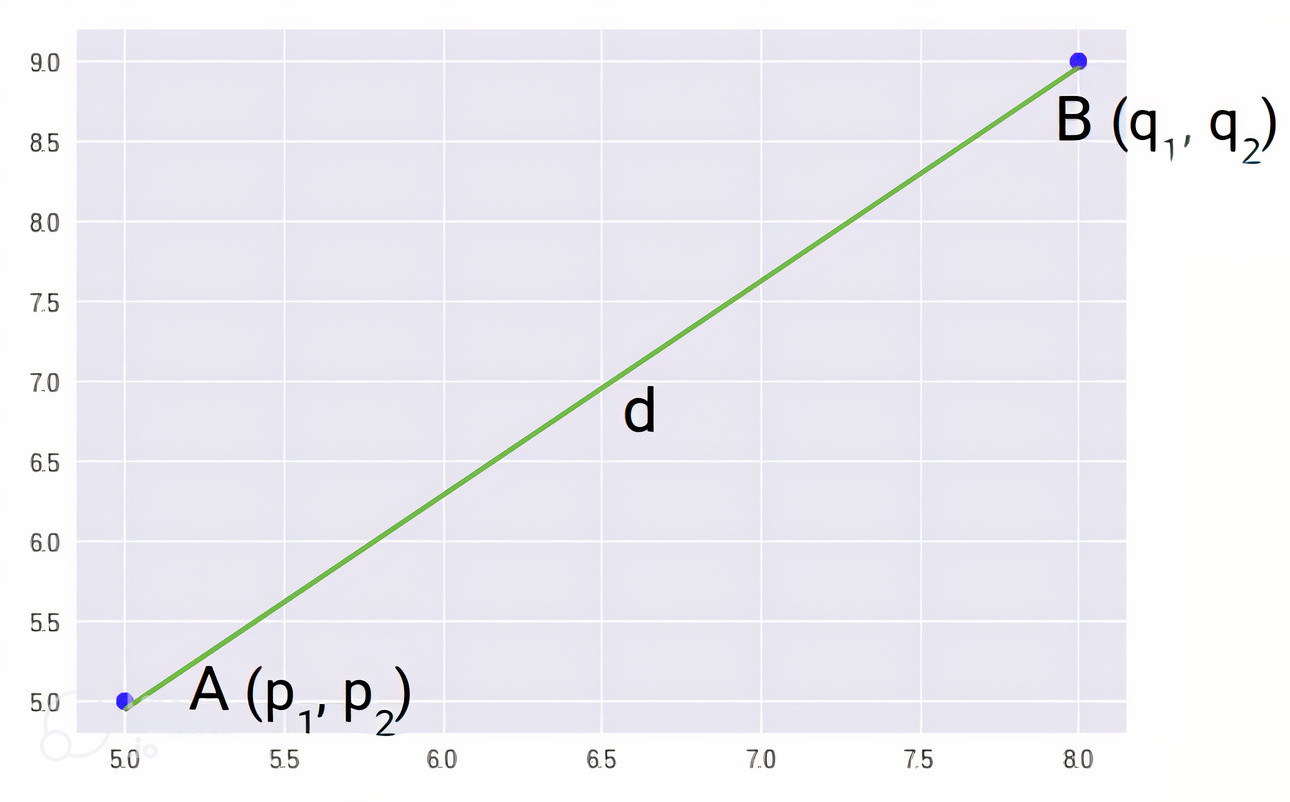
\includegraphics[width=0.75\linewidth]{figures/euclidean_distance}
	\caption{فاصله‌ی دو نقطه بر اساس فاصله‌ی اقلیدسی در دو بعد}\label{fig:euclidean_distance}
\end{figure}

\begin{equation} \label{d(p,q)}
	d\left( p,q\right) = \sqrt {\sum_{i=1}^{n} \left( q_{i}-p_{i}\right)^2 } 
\end{equation} 

\subsection{معیار فاصله‌ی ماهالانوبیس}
فاصله‌ی ماهالانوبیس\LTRfootnote[1]{Mahalanobis Distance}، فاصله‌ی بین دو نقطه در فضای چندمتغیره\LTRfootnote[2]{Multivariate Space} است. در یک فضای اقلیدسی منظم، متغیرها با محورهایی که در زوایای قائمه با یکدیگر ترسیم شده‌اند، نشان داده می‌شوند. فاصله‌ی بین هر دو نقطه را می‌توان با خط‌کش اندازه‌گیری کرد. برای متغیرهای غیر همبسته، فاصله‌ی اقلیدسی برابر با فاصله‌ی ماهالانوبیس است. با این ‌حال، اگر دو یا چند متغیر، همبسته باشند، محورها دیگر در زوایای قائم نیستند و اندازه‌گیری با یک خط‌کش غیرممکن می‌شود. علاوه بر این، اگر تعداد ابعاد بیشتر از سه باشد، دیگر در فضای سه‌ بعدی معمولی قابل ترسیم نخواهند بود. فاصله‌ی ماهالانوبیس، این مشکل اندازه‌گیری را حل می‌کند، زیرا فواصل بین نقاط را نسبت به یک مرکز اندازه‌گیری می‌کند. یک نقطه پایه یا مرکزی که می‌تواند به‌عنوان یک میانگین کلی برای داده‌های چند متغیره در نظر گرفته شود. هر چه فاصله‌ی ماهالانوبی بزرگ‌تر باشد، داده از مرکز دورتر است \cite{de2000mahalanobis}. نحوه‌ی محاسبه‌ی فاصله‌ی ماهالانوبیس در رابطه‌ی \ref{Delta} آمده است.\begin{figure}[h!]
	\centering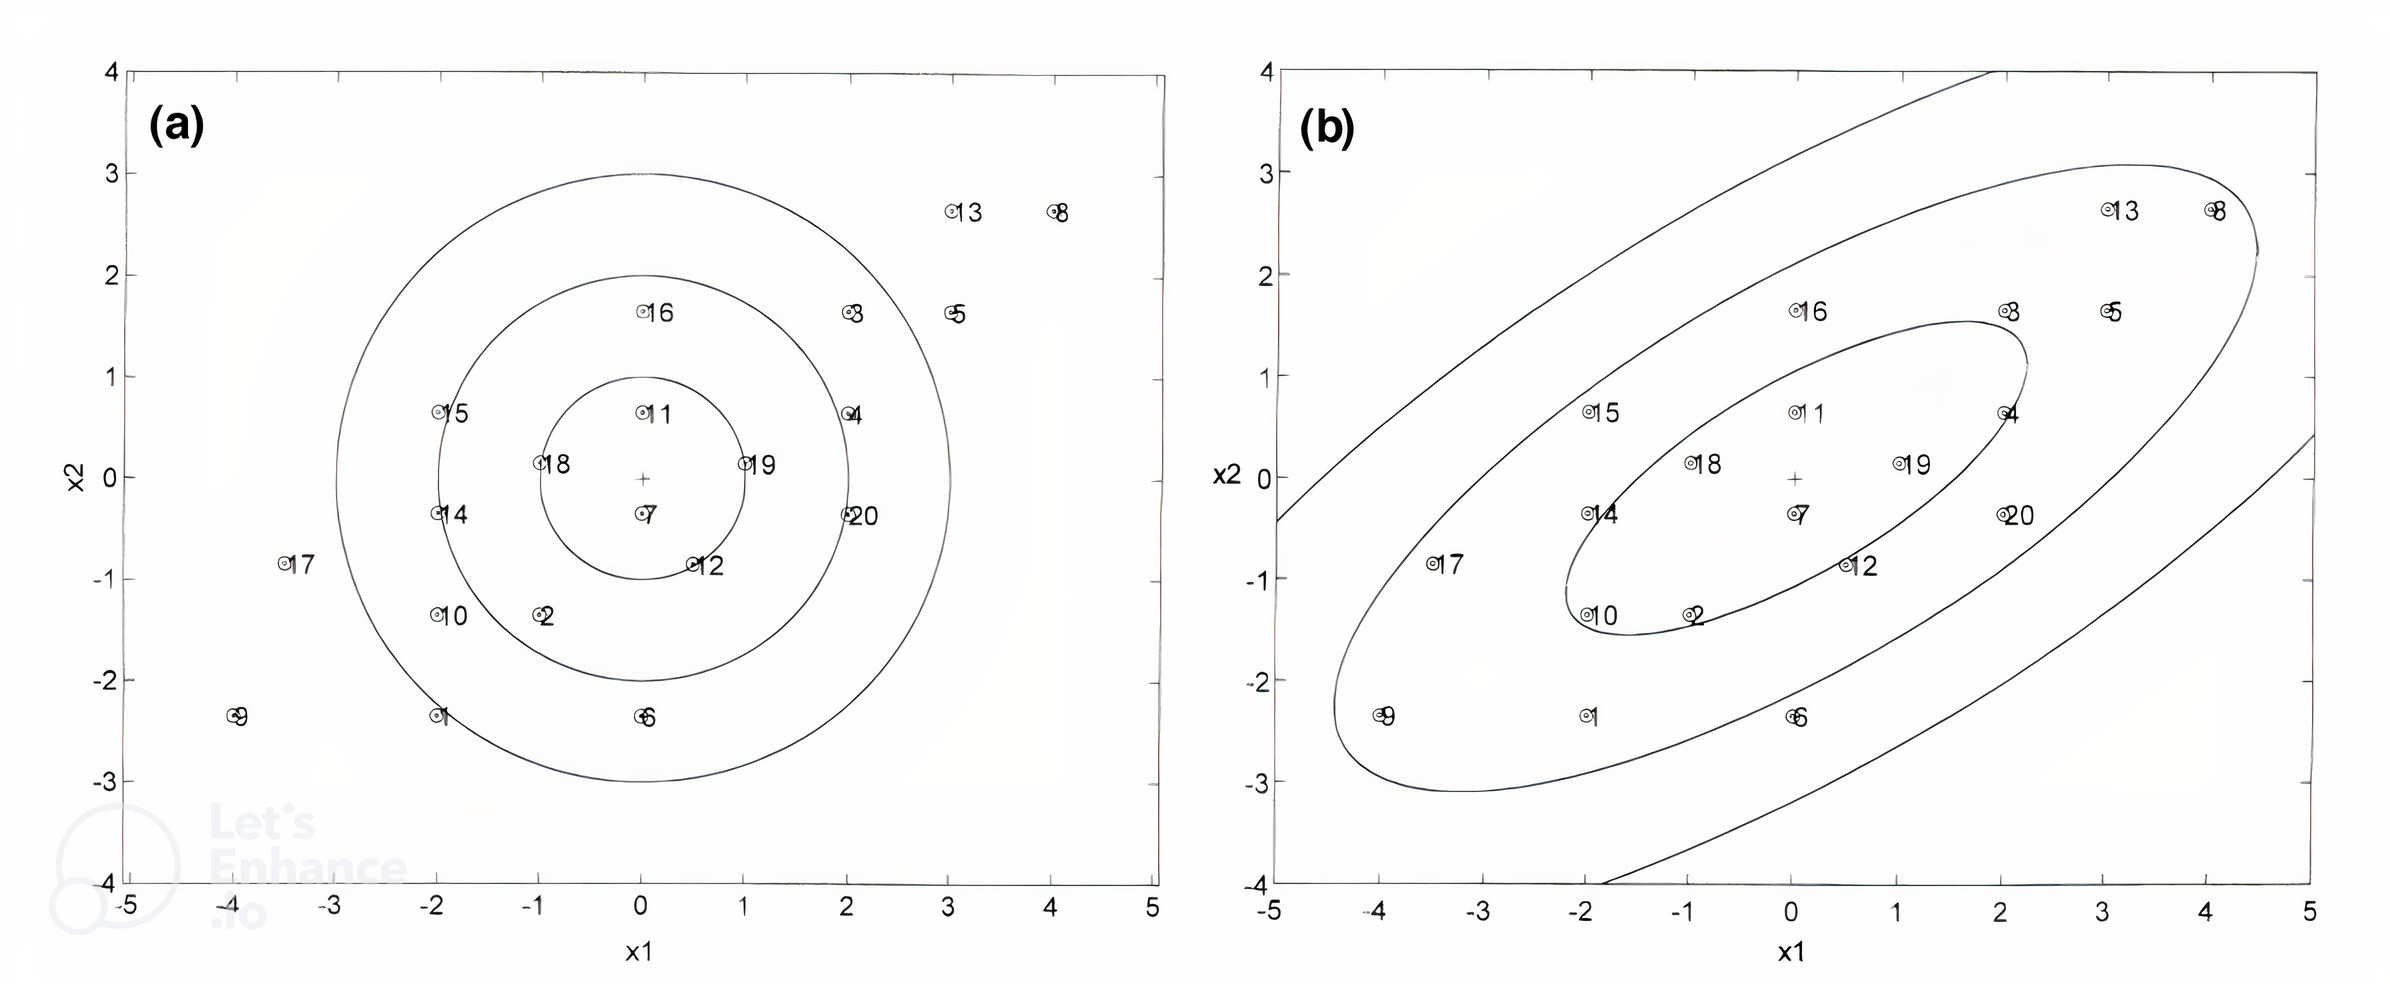
\includegraphics[width=1\linewidth]{figures/mahalanobis_figure}
	\caption{فاصله‌ی ماهالانوبیس حول یک نقطة مرکزی \cite{de2000mahalanobis}}\label{fig:mahalanobis_figure}
\end{figure} $\Sigma$ در فرمول زیر همان ماتریس کوواریانس است. در \cref{fig:mahalanobis_figure}، دو نمونه از محاسبه‌ی فاصله‌ی ماهالانوبیس برای تعدادی داده با دو متغیر \lr{x1} و \lr{x2} را مشاهده می‌کنید. همان‌طور که مشخص است فواصل تا یک نقطه‌ی مرکزی محاسبه شده است.  

\begin{equation} \label{Delta}
	\Delta^2 = \left( x-m\right)^\top\Sigma^{-1}\left( x-m\right)
\end{equation}

\subsection{خوشه‌بندی اقلیدسی}
خوشه‌بندی اقلیدسی\LTRfootnote{\lr{Euclidean Clustering}}، یک روش محبوب برای افراز یک ابر نقاط نامنظم به خوشه‌هایی کوچک‌تر است، که زمان لازم برای پردازش را به مراتب کاهش می‌دهد. این بازنمایی‌های خوشه‌ای، به فضای ابر نقاط نظم می‌دهند و برای زمانی که یک بازنمایی حجمی از فضای مسدود شده نیاز است، استفاده می‌شود. این روش برای زمانی که می‌خواهیم شکل اجسام تشخیص داده‌ شده در کادر محصورکننده را داشته باشیم نیز بسیار ارزشمند است. 

در عمل، برای پیدا کردن و بخش‌بندی\LTRfootnote{\lr{Segmentation}} خوشه اجسام متمایز،‌ معمولا از یک ساختار درخت کی‌دی\LTRfootnote{\lr{Kd-Tree}} استفاده می‌شود تا نزدیک‌‌ترین همسایه‌ها\LTRfootnote{\lr{Nearest Neighbours}} تشخیص داده شوند. الگوریتم این خوشه‌بندی به شکل زیر است:
\begin{enumerate}
    \item یک بازنمایی درخت کی‌دی برای ابر نقاط ورودی ساخته می‌شود $P$؛
    \item یک فهرست\LTRfootnote{List} از خوشه‌های خالی $C$ و یک صف\LTRfootnote{Queue} از نقاطی که بایستی بررسی شوند $Q$، ایجاد می‌شود؛
    \item به ازای هر نقطه $p_i \in P$، گام‌های زیر اجرا می‌شود:
    \begin{enumerate}
        \item نقطه $(p_i)$ را به صف اضافه کن؛
        \item به ازای هر نقطه $p_i \in Q$،‌ گام‌های زیر را انجام بده:
        \begin{itemize}
            \item در مجموعه نقاط همسایگی $P^k_i$، به دنبال نقاطی که در فاصله $r \l d_th$ هستند، جستجو کن؛
            \item به ازای هر همسایگی $p^k_i \in P^k_i$، بررسی کن که آیا نقطه قبلا پردازش شده است یا نه؛ اگر نه، آن را به صف $Q$ اضافه کن؛
        \end{itemize}
        \item زمانی که تمام نقاط داخل صف $Q$ پردازش شدند، $Q$ را به فهرست خوشه‌ها $C$ اضافه کن و $Q$ را خالی کن.
    \end{enumerate}
    \item الگوریتم زمانی خاتمه می‌یابد که تمام نقاط $p_i \in P$، پردازش شده باشند و عضو فهرست خوشه‌های $C$ شده باشند \LTRfootnote{\url{https://pcl.readthedocs.io/projects/tutorials/en/master/cluster_extraction.html}}.
\end{enumerate}

\subsection{مدل‌سازی سه‌بعدی}

مدل‌سازی سه‌بعدی هنر و علمی است که به ایجاد نمایش‌های دیجیتالی سه‌بعدی اجسام، صحنه‌ها یا محیط‌ها می‌پردازد. این تکنیک حیاتی در زمینه‌های مختلفی از جمله گرافیک کامپیوتری، انیمیشن، معماری، طراحی محصول و واقعیت مجازی به کار گرفته می‌شود. در دنیای مدل‌سازی سه‌بعدی، هنرمندان و طراحان از ابزارهای نرم‌افزاری ویژه برای ساخت مدل‌های سه‌بعدی با دقت و واقع‌گرایی بالا استفاده می‌کنند که قابلیت تغییر و مشاهده از زوایای مختلف را دارند. این مدل‌ها می‌توانند از اشکال هندسی ساده تا شخصیت‌های پیچیده، ساختارهای معماری یا جهان‌های مجازی کامل متغیر باشند. مدل‌سازی سه‌بعدی به عنوان پایه‌ای برای بسیاری از کاربردها عمل می‌کند و امکان ایجاد شخصیت‌های بازی ویدئویی واقع‌گرایانه، تصویرسازی طراحی‌های معماری، شبیه‌سازی پدیده‌های فیزیکی و بسیاری دیگر امکان‌پذیر می‌کند. با تنوع کاربردهای خود، مدل‌سازی سه‌بعدی نیرویی پیشرانه در عصر دیجیتال است که مرزهای خلاقیت و نوآوری را گسترش می‌دهد.

یکی از جنبه‌های کلیدی مدل‌سازی سه‌بعدی نمایش اجسام در فضای سه‌بعدی است، که معمولاً با استفاده از مختصات محورهای کارتزین تعریف می‌شود. این نمایش مکانی امکان ایجاد تجربیات جاذبه‌ای و تعاملی را فراهم می‌کند، زیرا مدل‌های سه‌بعدی می‌توانند برای شبیه‌سازی وضعیت‌های واقعی جهان، کاوش محیط‌های مجازی و انتقال اطلاعات پیچیده مورد استفاده قرار گیرند. برای مثال، توسعه شخصیت‌های واقع‌گرایانه برای فیلم‌های انیمیشنی، تجسم طراحی‌های معماری یا تجزیه و تحلیل داده‌های علمی، مدل‌سازی سه‌بعدی نقش اساسی در احیای ایده‌ها و مفاهیم در دنیای دیجیتال ایفا می‌کند. با پیشرفت فناوری، تکنیک‌های مدل‌سازی سه‌بعدی نیز تکامل می‌کنند و فرصت‌های جدیدی برای خلاقیت و حل مسائل در صنایع مختلف ارائه می‌دهند.

\begin{figure}[h]
    \centering
    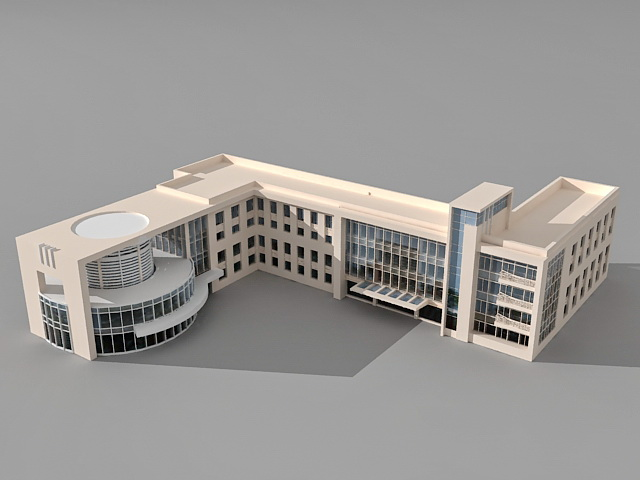
\includegraphics[width=0.7\linewidth]{3D_Model.png}
    \caption{مدل سه‌بعدی یک ساختمان}
    \label{fig:3D_Model}
\end{figure}


\section{نگاهی بر کار‌های پیشین}

در این بخش نگاهی مختصر به پژوهش‌هایی می‌اندازیم که علم دوقلوهای دیجیتال و نحوه ساختن آن را به چالش می‌کشند.

\subsection{طراحی سیستماتیک دوقلوی دیجیتال}

تحقیقات گوناگونی در زمینه طراحی سیستماتیک دوقلوی دیجیتال وجود دارند. در سال 2019، گروهی از محققین دانشگاه کمبریج\LTRfootnote{\lr{University of Cambridge}} اقدام به ساخت دوقلوی دیجیتالی از پردیس غربی کمبریج کردند \cite{lu2020developing}. در این مقاله، تمرکز اصلی بر روی عقب بودن عمران، معماری و مدیریت سازه\LTRfootnote{\lr{AEC/FM}} از تکنولوژی و عدم بکارگیری دوقلوهای دیجیتالی برای پیاده‌سازی پروژه‌های ساختمانی است. در این مقاله آمده است که در سال 2017، دولت بریتانیا پیشنهادی مبتنی بر ساختن دوقلوی دیجیتالی از کشور مطرح کرد و طبق گزارش‌های منتشر شده، این اقدام نیازمند آن است که شرکت‌های عمرانی و معماری، دوقلوی دیجیتال سازه‌های خود را تهیه نمایند. برای پیاده‌سازی دوقلوی دیجیتال از یک کشور، بایستی از هزاران دوقلوی دیجیتالی کوچک‌تر مانند دوقلوی دیجیتالی شهری و ساختمانی و جاده‌ای بهره برد. در ادامه شکل 1-2 از نحوه شکل‌گیری دوقلوی دیجیتالی برای یک کشور آورده شده است:

\begin{figure}[h]
	\centering
	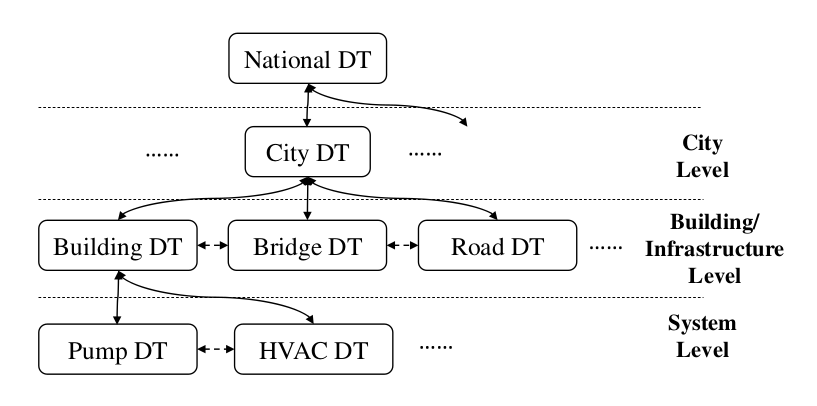
\includegraphics[scale=0.4]{figures/DT connections and hierarchy among different levels.png}
	\caption{  معماری دوقلوهای دیجیتالی و سلسله مراتب آنها \cite{lu2020developing}}
	\label{fig:dt_connections_and_hierarchy}
\end{figure}

با توجه به \cref{fig:dt_connections_and_hierarchy}، می‌توان دریافت کرد که دوقلوی‌ دیجیتال یک مجموعه بزرگ مانند کشور یا شهر، از دوقلو‌های دیجیتال کوچک‌تری شکل گرفته است. این مقاله به طراحی دوقلوی دیجیتال در ابعاد کوچک می‌پردازد که راه و روش‌های ایجاد دوقلوی دیجیتال پردیس دانشگاه را بررسی می‌کند.
این مقاله، اولین مقاله‌ای است که به طور سیستماتیک ساختن یک مدل از پردیس دانشگاه را انجام داده است و مراحل طراحی و معماری دوقلوی دیجیتال خود را به ساختن یک شهر یا کشور دیجیتالی براساس مقاله‌های گوناگون تعمیم داده است و تمامی محققان را در بکارگیری از این معماری تشویق کرده‌ است. 

\subsection{نحوه‌ی بهینه‌ مدل‌سازی سه‌بعدی دوقلوهای دیجیتال}

در مقاله‌‌ای دیگر که در سال ۲۰۲۲ توسط محققین دانشگاه تگزاس ال پاسو\LTRfootnote{\lr{University of Texas El Paso}} منتشر شده است،‌ یک روش عملی و کارآمد برای ایجاد دوقلوی دیجیتال هر مکان جغرافیایی، بخصوص دوقلوی دیجیتال دانشگاه‌ها و شبکه‌ی جاده‌ها معرفی شده است \cite{azfar2022efficient}. نویسندگان این مقاله، به چالش‌هایی که محققین گوناگون در ایجاد مدل‌های سه‌بعدی دقیق روبه‌رو می‌شوند را مورد تاکید کرده است و اهمیت تصویرسازی و شبیه‌سازی در تحقیقات دوقلوهای دیجیتال را بیان می‌کنند. آن‌ها یک جریان کاری ارائه می‌دهند که از داده‌ سرویس ‌\lr{OSM}\LTRfootnote{\lr{OpenStreetMap}} به عنوان پایه برای مدل‌سازی شبکه‌های جاده استفاده می‌کند و روشی برای ادغام اطلاعات زمینه‌ای مانند ساختمان‌ها و پستی بلندی\LTRfootnote{\lr{Terrain}} ارائه می‌دهد. این مقاله در مورد کاربرد‌های این روش در حوزه‌های مختلف همانند طراحی شبکه‌های جاده، شبیه‌سازی‌ خودرو‌های خودران با ابزار‌هایی مانند سومو\LTRfootnote{\lr{SUMO}} و کارلا\LTRfootnote{\lr{CARLA}} و  بخصوص در مورد تحقیقات بینایی کامپیوتر\LTRfootnote{\lr{Computer Vision}}  در محیط‌های دیجیتال و مصنوعی صبحت می‌کند. سپس این مقاله با برجسته کردن قابلیت چند‌منظوره بودن، مقیاس‌ پذیری و انعطاف پذیری روش پیشنهادی برای تحقیقات مختلف به پایان می‌رسد. این مقاله تاکید می‌کند که این رویکرد برای مدل‌سازی، شبیه‌سازی و تصویر‌سازی سه‌بعدی، بهره‌وری و کارآمدی دارد در حیطه‌های مختلف مانند حمل‌ و نقل، زیرساخت و بینایی کامپیوتر مفید و مقرون به صرفه است.

\begin{figure}[h]
	\centering
	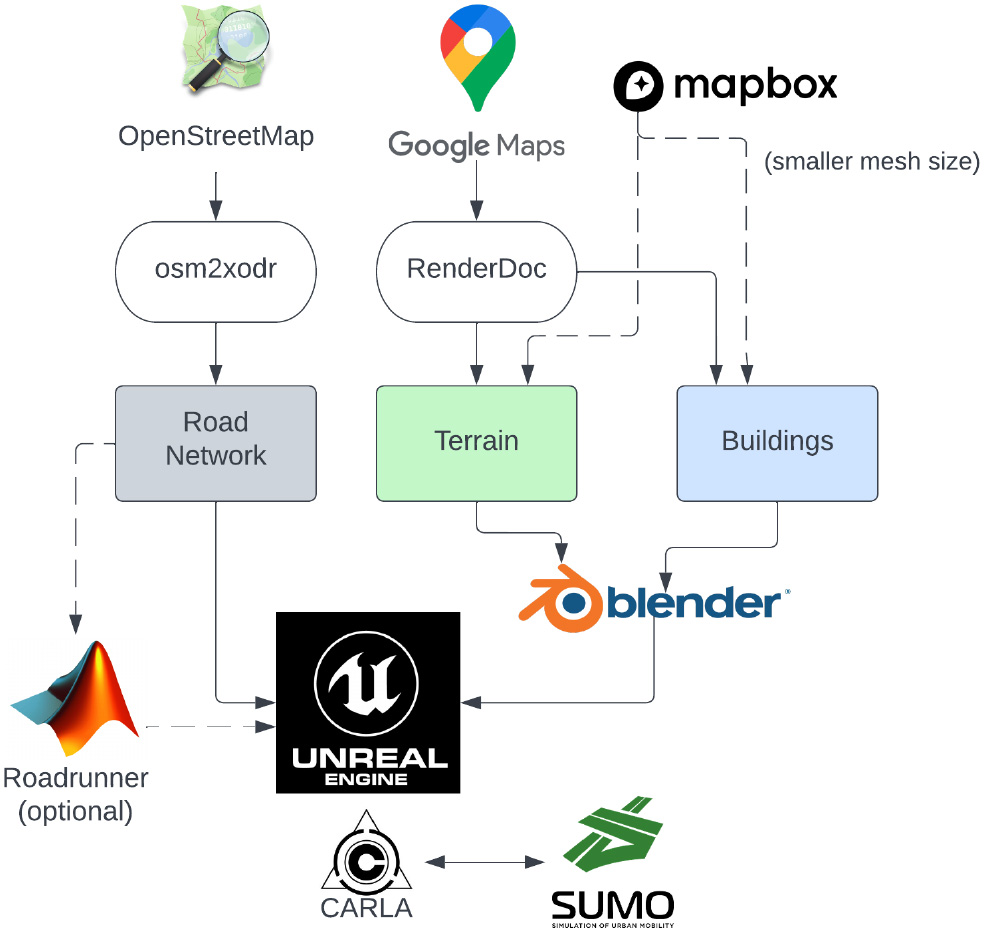
\includegraphics[scale=0.24]{figures/Digital_Twin_Procedure.png}
	\caption{  خلاصه‌ای از روش پیشنهاد شده برای ایجاد دوقلوی دیجیتال یک منطقه (در فصل چهارم به تحلیل دقیق این شکل می‌پردازیم) \cite{azfar2022efficient}}
	\label{fig:dt_procedure}
\end{figure}

\subsection{چرخه‌ی شبیه‌سازی خودکار اجسام پویا در دوقلوهای دیجیتال}

مقاله‌‌‌های دیگری نیز در زمینه تولید خودکار دوقلوی دیجیتال از یک جاده وجود دارند. مقاله‌‌ای در سال 2022 منتشر شده است که در زمینه ساخته شدن خودکار مدل‌های دوقلوی دیجیتالی صحنه‌های ترافیکی تحقیق می‌کند \cite{wang2022automatic}. در این مقاله با استفاده از حسگرهای لایدار و ابر نقاط، محیط اطراف با استفاده از خوشه بندی با مقیاس فاصله اقلیدسی\LTRfootnote{\lr{Euclidean Clustering}} دسته‌بندی می‌شود و براساس داده‌های پردازش شده از خوشه‌‌ها، دوقلوی دیجیتال ساخته می‌شود. \cref{fig:automatic_dt_creation_cycle} مراحل طی شده برای شکل‌گیری خودکار دوقلوی دیجیتال را نشان می‌دهد.

\begin{figure}[h]
	\centering
	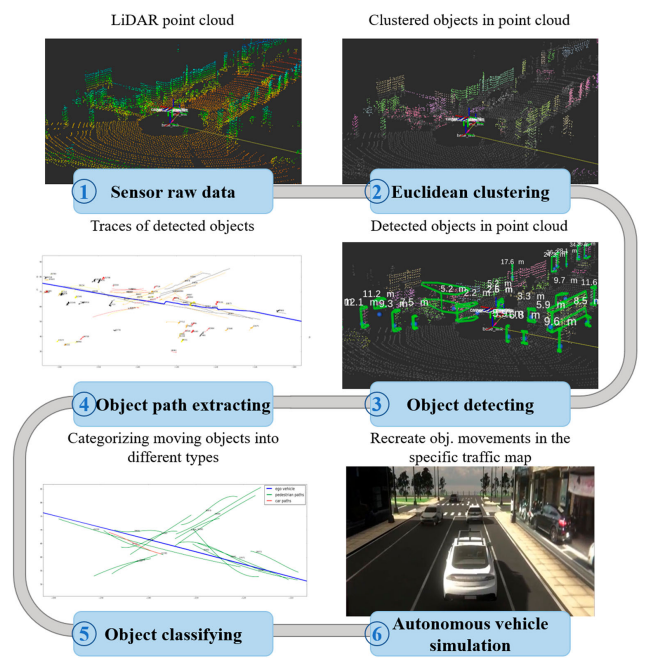
\includegraphics[scale=0.87]{figures/Automatic_DT_Creation_Cycle.png}
	\caption{  چرخه پردازش داده و تشخیص پارامترهای پویا و ساختن دوقلوی دیجیتال به صورت خودکار \cite{wang2022automatic}}
	\label{fig:automatic_dt_creation_cycle}
\end{figure}

حال به شرح هر کدام از بخش‌های \cref{fig:automatic_dt_creation_cycle} می‌پردازیم:
\begin{enumerate}
    \item برداشت اطلاعات سه بعدی از حسگر لایدار و ارسال اطلاعات در فرمت ابر نقاط به سرور
    \item از الگوریتم خوشه‌بندی با مقیاس فاصله اقلیدسی بر روی ابر نقاط برای تشخیص اجسام استفاده می‌شود. همچنین شناسه‌ای برای هر خوشه تشخیص داده شده در نظر گرفته می‌شود تا در مراحل بعدی جهت حرکت اجسام تشخیص داده شود.
    \item با استفاده از الگوریتم‌های تشخیص اجسام براساس کادر محصورکننده خوشه‌ها\LTRfootnote{\lr{Bounding-Box Based Detection Algorithms}}، اجسام خوشه‌بندی شده برچسب‌ گذاری می‌شوند و اجسامی که کادر محصورکننده آن‌ها بیشتر از کمینه تعیین شده توسط الگوریتم نباشد فیلتر می‌شوند (به علت‌های گوناگون ممکن است خوشه‌هایی وجود داشته باشد که شئ واقعی نباشند). همچنین جهت قرارگیری جسم، ثابت یا متحرک بودن جسم و جهت حرکت جسم تشخیص داده می‌شود.
    \item محاسبه مسیر حرکتی اجسام تشخیص داده‌ شده با تعیین موقعیت آن جسم در طول زمان
    \item دسته‌بندی اجسام براساس اندازه کادر محصورکننده به دسته‌های خودرو، موتورسیکلت و عابر پیاده
    \item پارامترهای گوناگون تشخیص داده شده در مراحل قبل بایستی پردازش شوند و مختصات و مسیر‌های حرکت اجسام تشخیص داده شده، به مختصات مدل سه بعدی شبیه‌سازی، تبدیل بشوند. در نهایت نیز مدل‌های سه بعدی اجسام براساس نوع آن جسم در نقشه مدل سه‌بعدی شبیه‌سازی با توجه به مختصاتشان قرار داده ‌می‌شوند و براساس مسیر حرکت خود، شروع به حرکت می‌کنند. حال می‌توان سیستم‌های ماشین‌ خودران را در این بستر ایجاد شده آزمود.
\end{enumerate}

مشاهده کردیم که هر کدام از مقالات، به دنبال مطرح کردن روشی سیستماتیک برای پیاده‌سازی دوقلو‌های دیجیتال هستند. همچنین مشاهده کردیم که در سال ۲۰۲۲ تحقیقاتی در زمینه خودکار کردن این پروسه صورت گرفته است. این پایان‌نامه نیز با الهام گیری از مقالات فوق، اقدام به پیاده‌سازی دوقلویی دیجیتال کرده است.
\chapter{ابزارها و کتابخانه‌ها}

در این فصل، نگاهی به تمام ابزار‌ها و کتابخانه‌‌های مورد استفاده پروژه می‌اندازیم. دانستن نحوه معماری و کارکرد این ابزارها، برای درک فصل طراحی و پیاده‌سازی پروژه، ضروری است.

\section{\lr{ROS}}
\lr{ROS}\LTRfootnote{\lr{Robot Operating System}}، مجموعه‌ای از کتابخانه‌های نرم‌افزاری و ابزارها است که در زمینه پیاده‌سازی ربات‌ها فعالیت ‌می‌کنند. \lr{ROS} یک بسته توسعه نرم‌افزار\LTRfootnote{\lr{Software Development Kit (SDK)}} ربات متن‌باز\LTRfootnote{\lr{Open Source}} است. این نرم‌افزار،‌ یک سکوی نرم‌افزاری را در دسترس توسعه‌گران صنعت رباتیک گذاشته است تا به تحقیقات، نمونه‌سازی‌ و گسترش علم رباتیک سرعت بخشد. 
\lr{ROS} بیش از ۱۰ سال است که در صنعت رباتیک، توسط میلیون‌ها توسعه‌گر در حال استفاده است. این نرم‌افزار، در اکثر سیستم‌ عامل‌ها و سیستم‌های نهفته\LTRfootnote{\lr{Embedded Systems}} قابل توسعه است، و در حوزه‌های پردازش بلادرنگ نیز نقشی اساسی دارد \cite{doi:10.1126/scirobotics.abm6074}.

\subsection{اکوسیستم}
برخلاف اسم ‌آن، \lr{ROS} یک سیستم‌ عامل نیست و همانطور که ذکر شد، یک بسته توسعه نرم‌افزار ربات است. اکوسیستم این بسته نرم‌افزاری به شکل زیر است:

\begin{figure}[h!]
    \centering
    
\includegraphics[width=1\linewidth]{figures/ROS_Ecosystem.png}
    \caption{تصویری از اجزای \lr{ROS} \cite{ROS:2023}}
    \label{fig:ROS_ecosystem}
\end{figure}

همانطور که مشاهده ‌می‌کنیم، اکوسیستم نرم‌افزار \lr{ROS} از چهار بخش اساسی تشکیل شده است:
\begin{enumerate}
    \item \textbf{لوله‌کشی}\LTRfootnote{\lr{Plumbing}}: در اصل، \lr{ROS} یک سیستم انتقال پیام فراهم می‌کند که اغلب به عنوان "میان‌افزار\LTRfootnote{\lr{Middleware}}" یا "لوله‌کشی" شناخته می‌شود. ارتباط اولین نیازی است که هنگام پیاده‌سازی یک برنامه رباتیک جدید یا به طور کلی هر سیستم نرم‌افزاری که با سخت‌افزار تعامل خواهد داشت، به وجود می‌آید. سیستم پیام‌دهی محبوب و تست‌شده‌ \lr{ROS}، باعث صرفه جویی در زمانی می‌شود که برای مدیریت جزئیات مربوط به ارتباط بین گره‌های\LTRfootnote{\lr{Nodes}} توزیع‌شده،‌ صرف شده است (از طریق یک الگوی انتشار/اشتراک ناشناس\LTRfootnote{\lr{Anonymous Publish/Subscribe Patterns}}). این رویکرد به شما کمک می‌کند تا شیوه‌های خوبی را در توسعه نرم‌افزار‌های خود رعایت کنید، که شامل جدا کردن ایرادها، جداسازی نیازمندی‌ها و رابط‌هایی\LTRfootnote{\lr{Interface}} واضح می‌شود. استفاده از \lr{ROS} منجر به ایجاد سیستم‌هایی می‌شود که آنها را آسان‌تر برای نگهداری، مشارکت در توسعه، و استفاده مجدد می‌کند.
    
    در طی این مسیر، می‌توان از تجربیات جامعه گسترده‌ای که به ایجاد استانداردهای پیام \lr{ROS} منجر شده است، بهره برد. این استانداردها برای تعامل با همه چیز از سنجش فاصله لیزری و دوربین‌ها تا الگوریتم‌های موقعیت‌یابی و رابط‌های کاربری استفاده می‌شوند \cite{ROS:2023}.
    \item ابزار: پیاده‌سازی برنامه‌های رباتیک چالش‌برانگیز است. شما با تمام مشکلات هر تلاش توسعه نرم‌افزاری مواجه می‌شوید و علاوه بر آن، نیاز به ارتباط ناهمگام\LTRfootnote{\lr{Asynchronous Interaction}} با دنیای فیزیکی از طریق حسگرها و اعمال‌کننده‌ها هم به لیست مشکلات اضافه می‌شود. برای ساختن برنامه‌ها به صورت کارآمد، به ابزارهای توسعه‌دهنده خوبی نیاز است. \lr{ROS} این ابزارها را دارد که شامل ابزارهایی مانند راه‌اندازی\LTRfootnote{\lr{Launch}}، خودکاوی\LTRfootnote{\lr{Introspection}}، اشکال‌زدایی\LTRfootnote{\lr{Debugging}}، بصری‌سازی\LTRfootnote{\lr{Visualization}}، کشیدن نمودار، ثبت اتفاقات\LTRfootnote{\lr{Logging}} و پخش\LTRfootnote{\lr{Playback}} می‌شوند. این ابزارها به پیشرفت تیم‌های توسعه، شتاب می‌دهند و می‌توانند همراه محصول عرضه ‌شده قرار گیرند \cite{ROS:2023}.

    \item قابلیت‌ها: جامعه‌ی \lr{ROS} یک مجموعه‌ی نرم‌افزارهای رباتیک است. اگر نیاز به یک درایور برای دستگاه موقعیت‌یاب دارید، یا به یک کنترل کننده‌ی حرکت و تعادل برای ربات چهارپا، یا یک سیستم نقشه‌برداری برای ربات متحرکتان، \lr{ROS} ابزاری برای شما دارد. از درایورها تا الگوریتم‌ها و رابط‌های کاربری، \lr{ROS} اجزای اصلی را فراهم می‌کند که به شما اجازه می‌دهد تا بر روی برنامه‌ی خود تمرکز کنید. هدف پروژه‌ی \lr{ROS}، ارتقاء همیشگی استانداردهای رایج و از این راه کاهش مانع در توسعه برنامه‌های رباتیک است. هر کسی که یک ایده خوب برای یک ربات مفید (یا سرگرم‌کننده، یا جالب) دارد، باید بتواند آن ایده را بدون نیاز به درک تمامی اجزای نرم‌افزاری و سخت‌افزاری مرتبط آن، به واقعیت تبدیل کند \cite{ROS:2023}.

    \item جامعه: جامعه \lr{ROS} وسیع، متنوع و جهانی است. از آدم‌های علاقه‌مند عادی تا دانشجویان، حتی شرکت‌های بین‌المللی و دولت‌ها نیز از ‌\lr{ROS} برای توسعه تکنولوژی رباتیک استفاده می‌کنند.
\end{enumerate}

\subsection{نسخه‌ها}

نرم‌افزار \lr{ROS}، دو نسخه اصلی دارد که \lr{ROS1} و \lr{ROS2} نام دارند. امروزه بیشتر شرکت‌ها از نسخه \lr{ROS2} استفاده می‌کنند زیرا از نظر زیرساخت شبکه‌ای، امنیت و قابلیت‌های توسعه با استانداردهای امروزه، پیشرفته‌تر است. 
\begin{figure}[h!]
    \centering
    \includegraphics[width=0.8\linewidth]{figures/ROS1_ROS2_comparison.png}
    \caption{تفاوت قابلیت‌های \lr{ROS2} نسبت به \lr{ROS1}\cite{doi:10.1126/scirobotics.abm6074}}
    \label{fig:ROS1_ROS2_comparison}
\end{figure}

هر کدام از نسخه‌های \lr{ROS}، توزیع‌هایی\LTRfootnote{\lr{ROS Distributions}} را در اختیار توسعه‌دهندگان قرار داده‌اند. از آنجایی که در این پژوهش نیز از نسخه جدید‌تر \lr{ROS2} استفاده شده است. در \cref{fig:ROS2_Distributions} می‌توانیم چهار توزیع اصلی مورد استفاده توسعه‌دهندگان رباتیک را مشاهده کنیم. در این پژوهش، از توزیع \lr{ROS2 Humble} استفاده شده است که نسخه پایدار و بروز سال ۲۰۲۳ به حساب می‌آید.
\\
\\
\\
\begin{figure}[h]
    \centering
    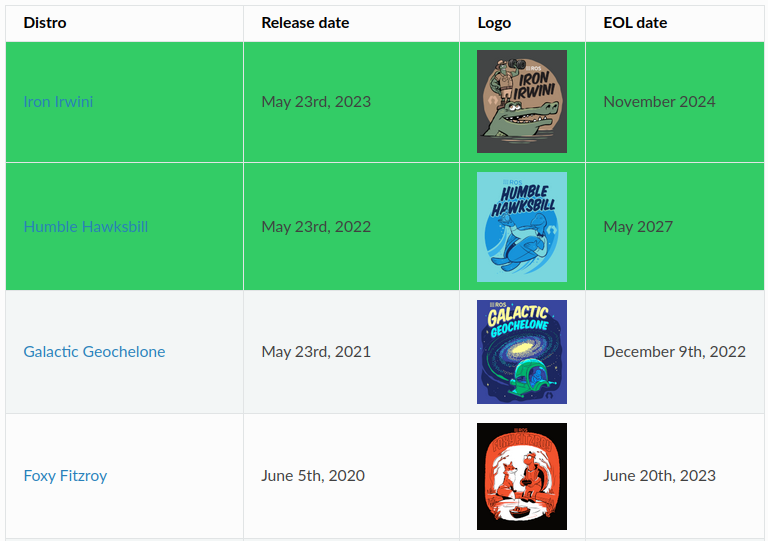
\includegraphics[width=0.8\linewidth]{figures/ROS2_Distributions.png}
    \caption{چهار توزیع اصلی \lr{ROS2}}
    \label{fig:ROS2_Distributions}
\end{figure}

\subsection{معماری بسته توسعه نرم‌افزار \lr{ROS2}}
هر نرم‌افزار توسعه شده توسط \lr{ROS2}، از چند اجزای اصلی تشکیل شده است که در ادامه با آنها آشنا خواهیم شد.

\subsubsection{گراف \lr{ROS2}}
گراف \lr{ROS2}\LTRfootnote{\lr{ROS2 Graph}}، شبکه‌ای از عناصر \lr{ROS2} است که در هم‌زمان در کنار یکدیگر داده‌ها را پردازش می‌کنند. این گراف شامل تمامی اتصالات شبکه‌ی داده‌ای و عناصر قابل اجرا است. 

\subsubsection{گره \lr{ROS2}}
گره \lr{ROS2}\LTRfootnote{\lr{ROS2 Node}}، یک شرکت‌کننده در گراف \lr{ROS2} که از یک کتابخانه کلاینت\LTRfootnote{\lr{Client Library}}، برای ارتباط با سایر گره‌ها استفاده می‌کند. گره‌ها می‌توانند با سایر گره‌ها در داخل همان فرایند، در یک فرایند متفاوت، یا در ماشین متفاوتی ارتباط برقرار می‌کنند. معمولا، گره‌ها واحد محاسباتی در یک گراف  \lr{ROS} هستند؛ هر گره باید یک کار منطقی انجام دهد.

گره‌ها می‌توانند داده‌های خود را به مبحثی\LTRfootnote{\lr{Topic}} انتشار کنند\LTRfootnote{\lr{Publish}} تا بقیه گره‌ها استفاده کنند، یا در موضوعی اشتراک داشته باشند\LTRfootnote{\lr{Subscribe}} و اطلاعات دریافت کنند. آن‌ها می‌توانند به عنوان یک سرویس‌ کلاینت\LTRfootnote{\lr{Service Client}} عمل کنند و محاسبات خود را بر عهده گره دیگری قرار دهند، یا خودشان یک سرویس سرور\LTRfootnote{\lr{Service Server}} باشند و کار محاسبات بقیه گره‌ها را بر عهده بگیرند. برای محاسباتی که طولانی هستند، این گره‌ها می‌توانند یک کلاینت عمل\LTRfootnote{\lr{Action Client}} باشند یا یک سرور عمل‌\LTRfootnote{\lr{Action Server}} باشند. گره‌ها می‌توانند پارامتر‌های\LTRfootnote{\lr{Parameters}} قابل تنظیمی داشته باشند که در حین اجرا توسط بقیه گره‌ها تنظیم شوند.
\begin{definition}
گره یک واحد سازمان‌دهنده مهم است که به کاربر امکان تفکر درباره یک سیستم پیچیده را می‌دهد \cite{doi:10.1126/scirobotics.abm6074}.
\end{definition}

\begin{figure}[h!]
    \centering
    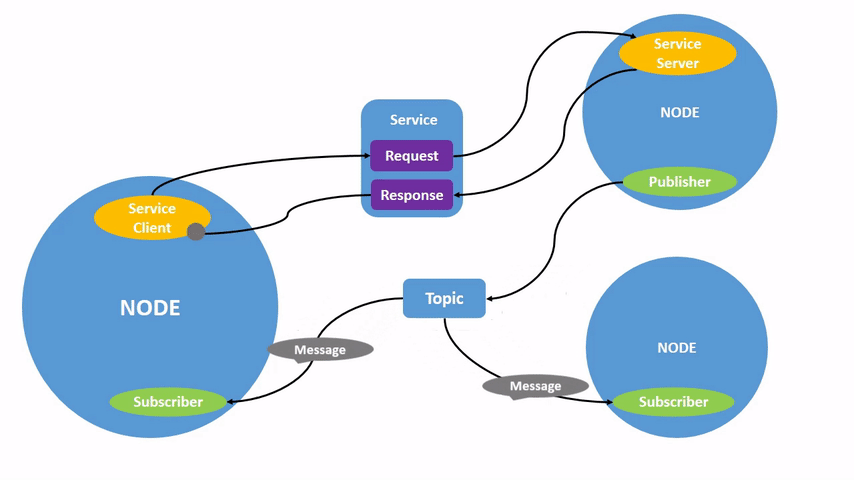
\includegraphics[width=0.75\linewidth]{figures/ROS2_Node_Graph.png}
    \caption{یک گراف ‌\lr{ROS2} ساده \cite{ROS2:Humble_Documentation}}
    \label{fig:ROS2_Node_Graph}
\end{figure}

\subsubsection{رابط‌ها}
تمامی برنامه‌ها و گره‌های توسعه شده تحت \lr{ROS}، از  سه نوع الگوی اصلی برای ارتباط استفاده می‌کنند:
\begin{itemize}
    \item \textbf{‌مبحث‌ها}: الگوی رایج‌تری که کاربران با آن تعامل می‌کنند، مبحث‌ها هستند که یک چارچوب انتقال پیام ناهمگام هستند. کاربران برای ارسال یا دریافت پیام از مبحث‌ها، بایستی از روش انتشار/اشتراک استفاده کنند. ‌\lr{ROS2} تمرکز خود را بر روی استفاده از پیام‌رسانی ناهمگام برای سازماندهی یک سیستم با رابطه‌های قوی متناظر گذاشته است و این کار را با سازماندهی نقاط پایانی\LTRfootnote{\lr{Endpoints}} در یک گراف محاسباتی تخت مفهوم گره انجام می‌دهد. معماری انتشار-اشتراک ناشناس، ارتباطات چند به چند\LTRfootnote{\lr{Many to Many}} را امکان‌پذیر می‌کند. یک توسعه‌دهنده می‌تواند با ایجاد یک اشتراک به یک مبحث، تمام پیام‌های عبوری از این مبحث را بدون اعمال تغییری در عملکرد آن، مشاهده کند \cite{doi:10.1126/scirobotics.abm6074}.
    \item \textbf{سرویس‌ها}: ارتباط ناهمگان همیشه بهترین ابزار نیست. \lr{ROS2} یک الگوی ارتباطی درخواست-پاسخ\LTRfootnote{\lr{Request-Response}}، به نام سرویس‌ها را نیز فراهم می‌کند. ارتباط درخواست-پاسخ تخصیص داده بین یک جفت درخواست و پاسخ را آسان می‌کند. به طور منحصر به فرد، \lr{ROS2} به یک پردازش‌گر سرویس اجازه می‌دهد که در طول یک فراخوانی به آن، مسدود\LTRfootnote{\lr{Blocking}} نشود که یعنی در‌خواست‌ها و پاسخ‌های دیگر هم بتوانند پردازش شوند و منتظر نمانند. سرویس‌ها نیز تحت گره‌ها سازماندهی می‌شوند \cite{doi:10.1126/scirobotics.abm6074}. 
    \item \textbf{اعمال}: اعمال، الگوی ارتباط منحصر‌ به‌ فرد \lr{ROS2} است. اعمال هدف محور هستند و ارتباط‌هایی ناهمگام با الگوی درخواست، پاسخ، و بازخورد دوره‌ای با قابلیت لغو هستند. این الگوی ارتباطی، در وظایف طولانی مانند مسیریابی خودکار یا مدیریت خودکار استفاده می‌شود، اگرچه کاربردهای دیگری هم دارد. مشابه سرویس‌ها، عمل‌ها بدون مسدود کردن هستند و تحت گره سازماندهی می‌شوند \cite{doi:10.1126/scirobotics.abm6074}.
\end{itemize}

\begin{figure}[h!]
    \centering
    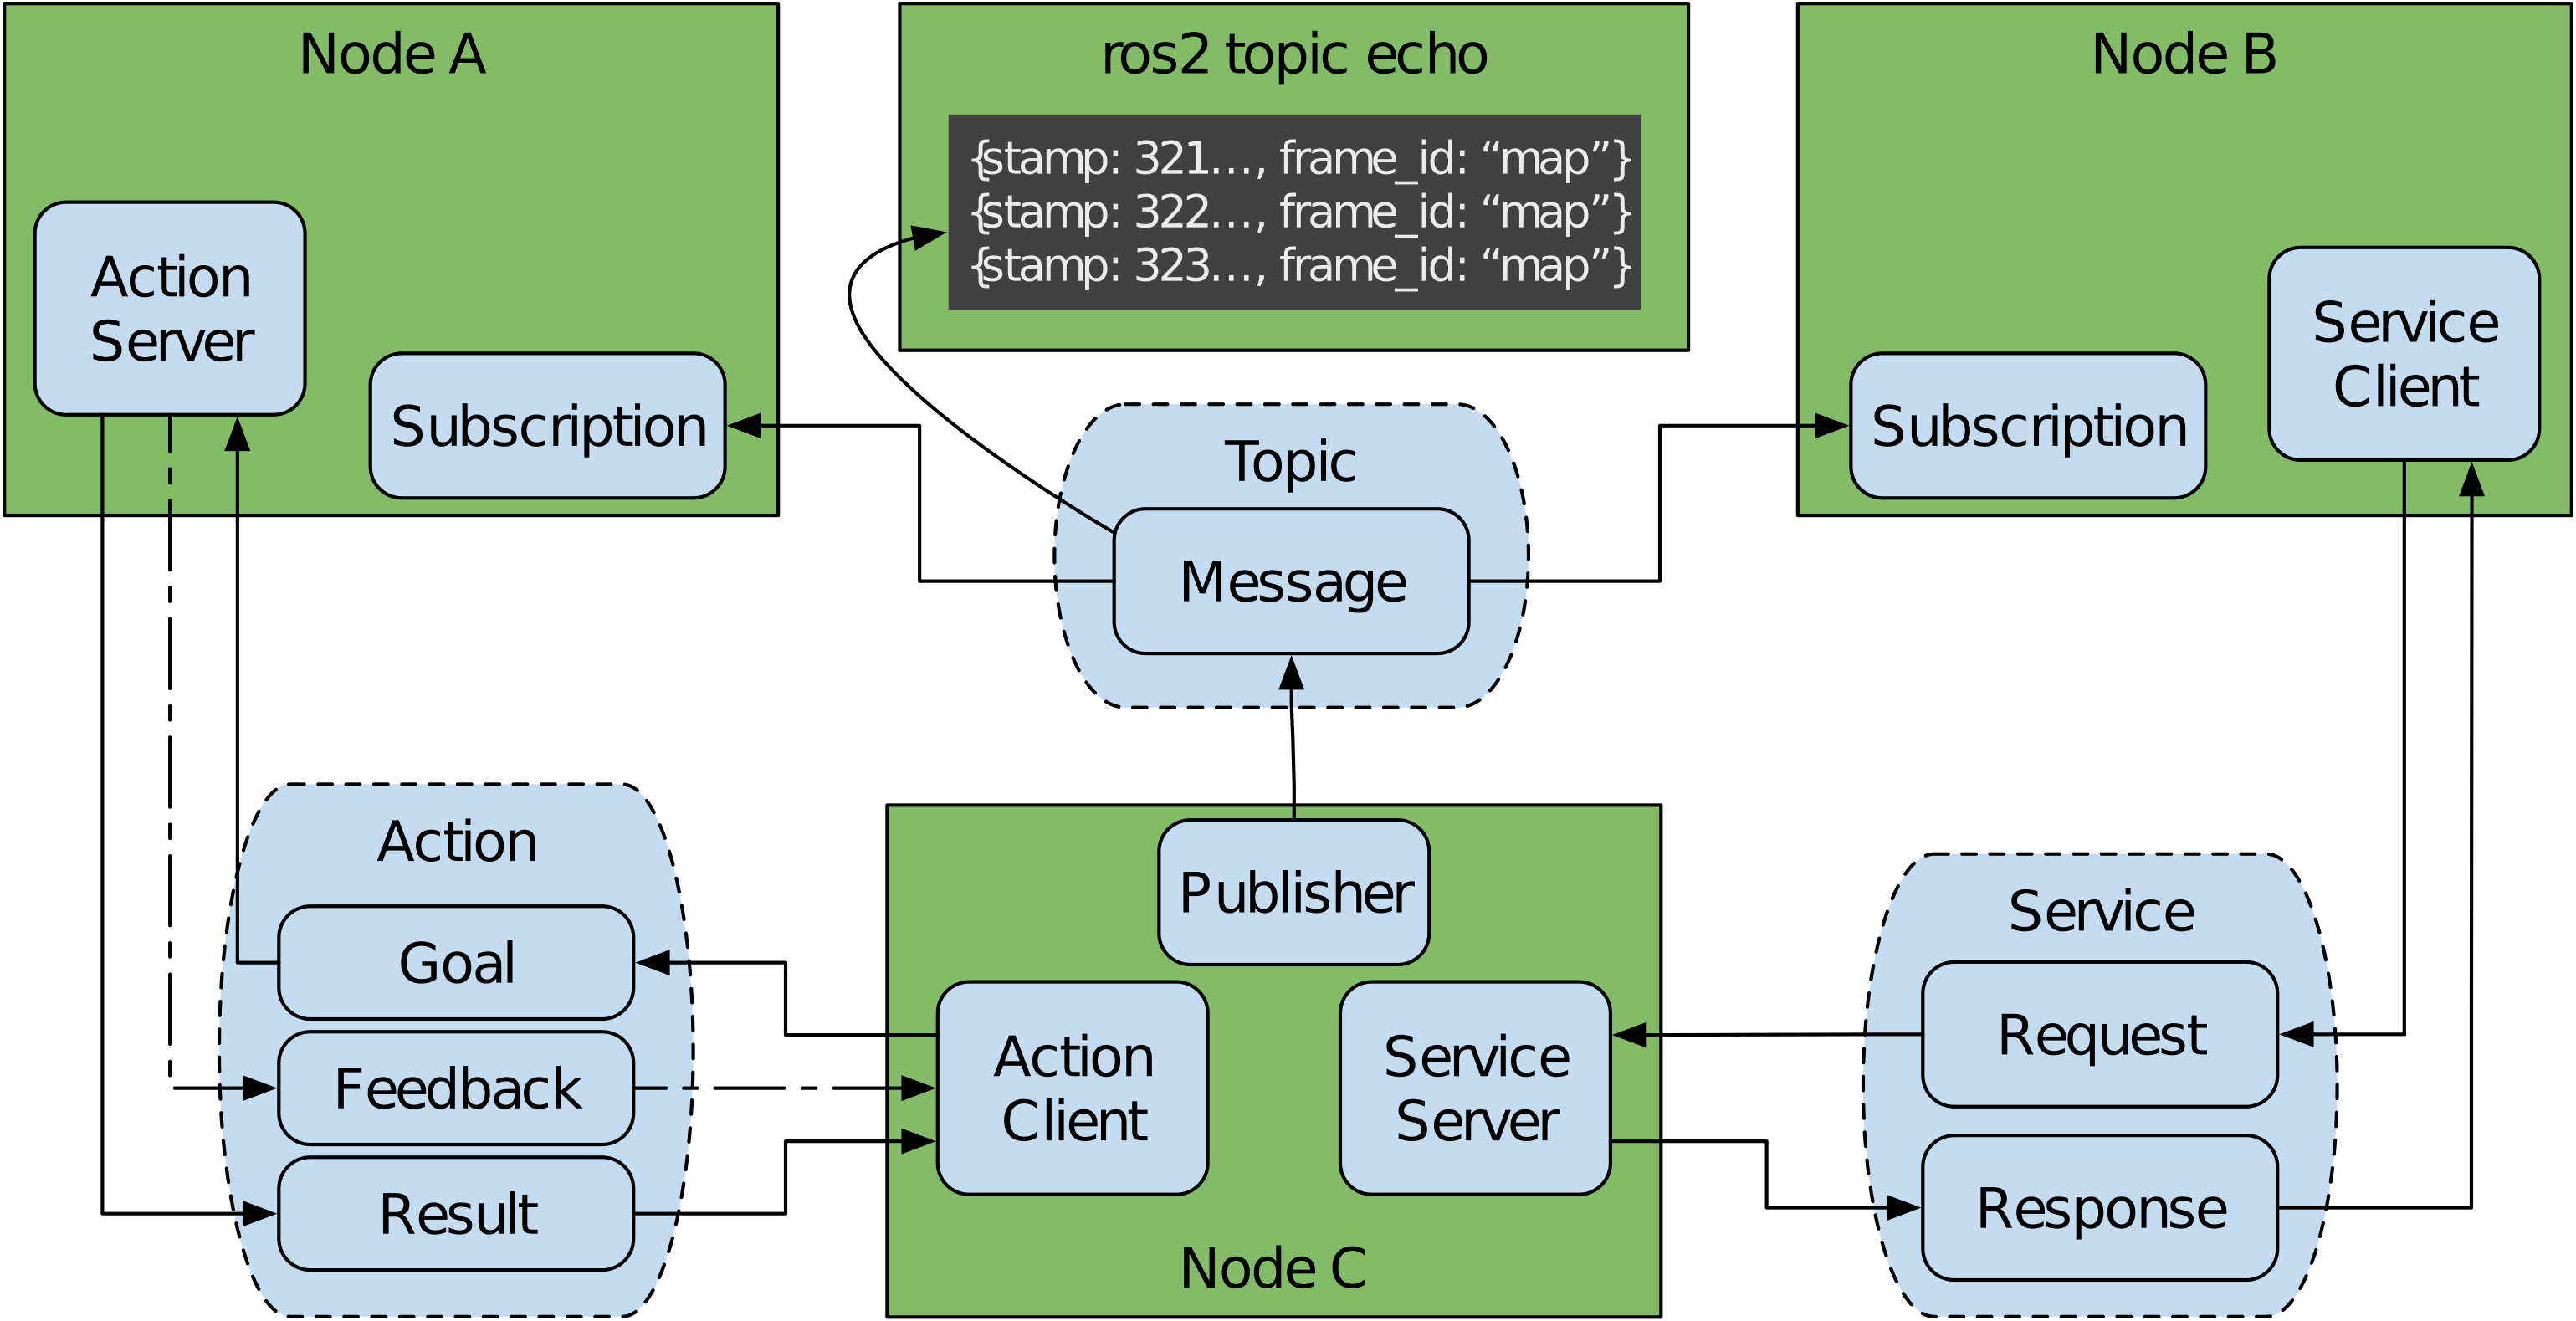
\includegraphics[width=1\linewidth]{figures/ROS2_Node_Interfaces.png}
    \caption{رابط‌های یک گره \lr{ROS2}: مبحث‌ها، سرویس‌ها، اعمال \cite{doi:10.1126/scirobotics.abm6074}}
    \label{fig:ROS2_Node_Interfaces}
\end{figure}

\subsubsection{کتابخانه‌های کلاینت}
کتابخانه‌های کلاینت،‌ واسط‌های برنامه‌نویسی هستند که به کاربران امکان پیاده‌سازی کد \lr{ROS2} را می‌دهند. با استفاده از کتابخانه‌های کلاینت،‌کاربران به مفاهیم مختلف مانند گره‌ها، مبحث‌ها، سرویس‌ها و اعمال دسترسی پیدا می‌کنند. کتابخانه‌های کلاینت، به انواع زبان‌های برنامه‌نویسی ارائه می‌شوند تا کاربران بتوانند کد ‌\lr{ROS2} خود را به زبانی که برای برنامه‌شان مناسب‌تر است،‌ بنویسند. به عنوان مثال، ممکن است کاربری بخواهد ابزار‌های تصویر‌سازی خود را با زبان پایتون\LTRfootnote{\lr{Python Programming Language}} نویسد چرا که سریع‌ترین تکرار نمونه‌سازی‌ها را داشته باشد؛ در حالی که برای بخش‌هایی از سیستم خود که به راندمان بیشتری نیاز دارد،‌ از زبان برنامه‌نویسی \lr{C++} استفاده کند  \cite{ROS2:Humble_Documentation}.

گره‌های نوشته شده با کتابخانه‌های کلاینت مختلف،‌ قادر به اشتراک‌گذاری پیام‌ها با یکدیگر هستند، زیرا تمام کتاب‌خانه‌های کلاینت \lr{ROS2}، مولدهای کدنویسی‌ای پیاده‌سازی کرده‌اند که به کاربران امکان تعامل با فایل‌های رابط \lr{ROS2}، به زبان مربوطه را می‌دهد (در فصل چهارم نیز اشاره‌ای به این موضوع می‌شود زیرا نیاز به استفاده از یک مولد است که بتوان یک سری از رابط‌های \lr{Autoware} را برای بسته‌ \lr{ROS2-For-Unity}، ترجمه کرد) \cite{ROS2:Humble_Documentation}.

\begin{figure}[h!]
    \centering
    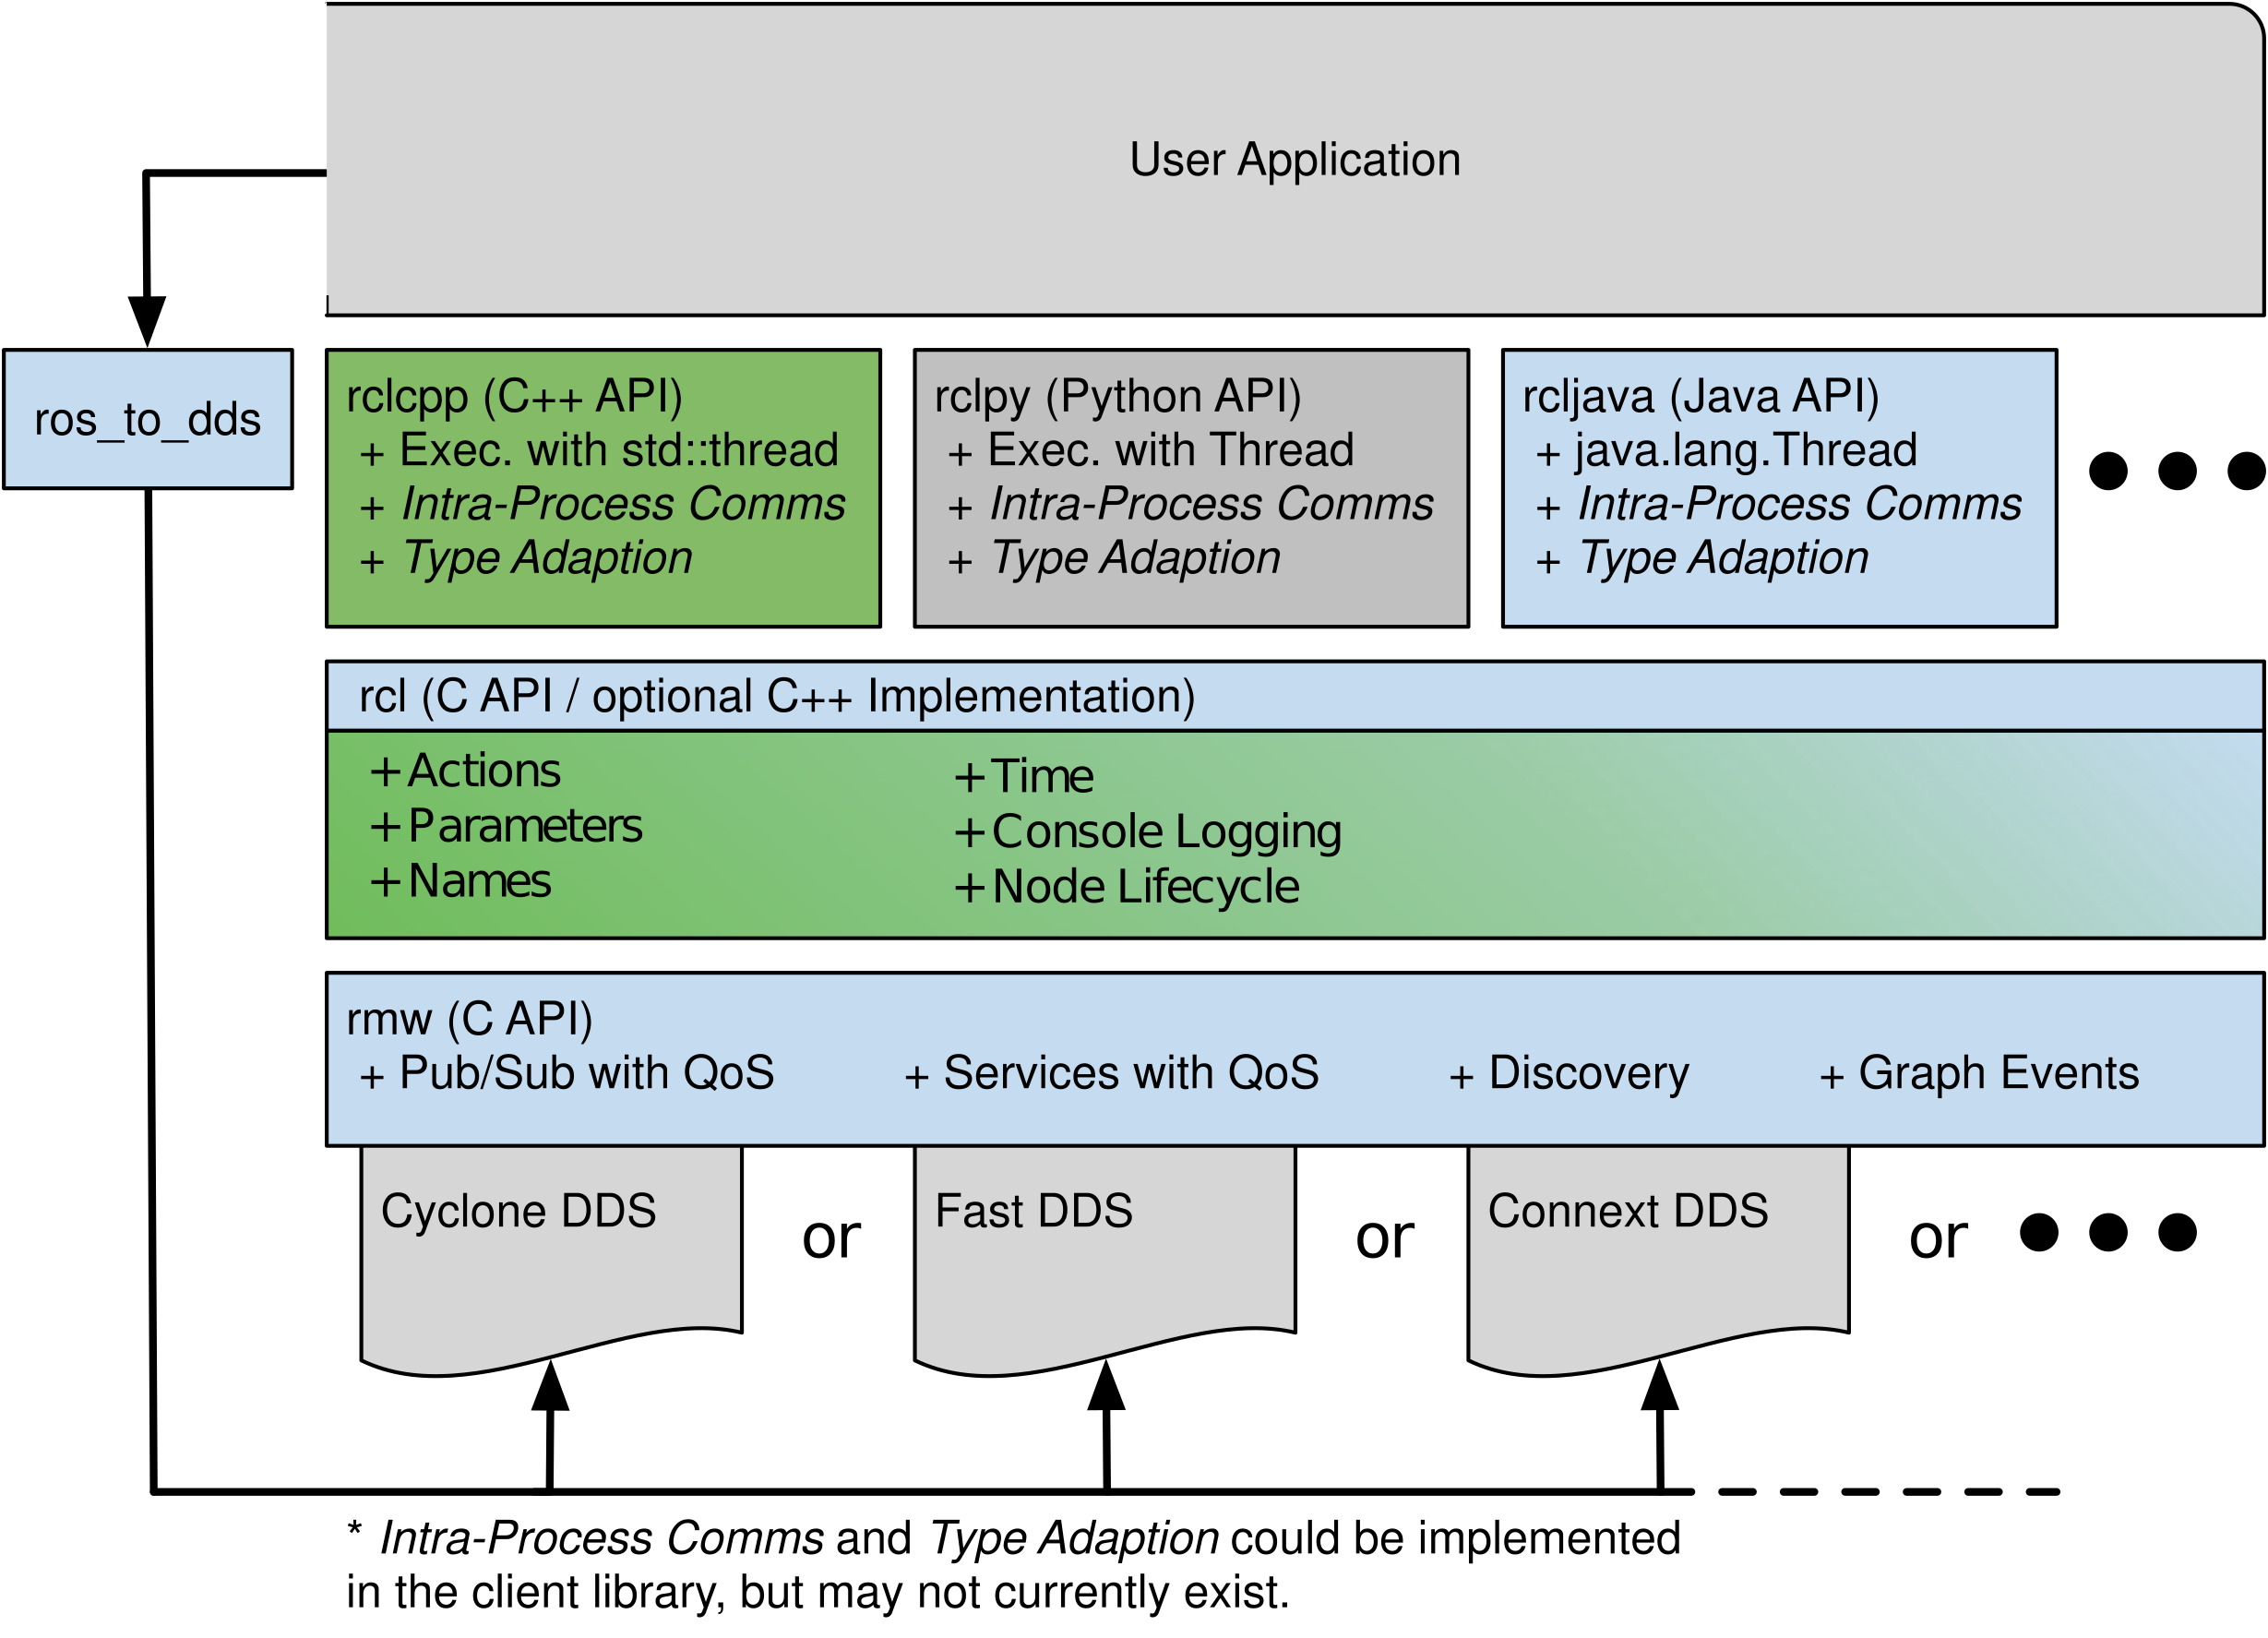
\includegraphics[width=1\linewidth]{figures/ROS2_Client_Library_API_Stack.png}
    \caption{کتابخانه‌های کلاینت \lr{ROS2} \cite{doi:10.1126/scirobotics.abm6074}}
    \label{fig:ROS2_Client_Library_API_Stack}
\end{figure}

علاوه بر ابزارهای ارتباطی مختص به زبان، کتابخانه‌های کلاینت به کاربران توانایی دسترسی به عملکرد اصلی‌ای که \lr{ROS} را به \lr{"ROS"} تبدیل می‌کند را ارائه می‌دهد. به عنوان مثال، در ادامه لیستی از عملکرد‌هایی آمده است که معمولا از طریق یک  کتابخانه کلاینت می‌توان به آنها دسترسی داشت \cite{ROS2:Humble_Documentation}:
\begin{itemize}
    \item نام‌ها و فضای نام‌ها\LTRfootnote{\lr{Namespaces}}
    \item زمان (واقعی یا شبیه‌سازی)
    \item پارامترها
    \item ثبت وقایع کنسول
    \item مدل موازی‌سازی نخ‌ها\LTRfootnote{\lr{Threading Model}}
    \item ارتباط داخلی فرایند‌ها
\end{itemize}

در \cref{fig:ROS2_Client_Library_API_Stack} نیز می‌توان کلیات نحوه کارکرد کتابخانه‌های کلاینت را مشاهده کرد.

\section{\lr{Autoware}}
نرم‌افزار \lr{Autoware} از شرکت \lr{AWF}\LTRfootnote{\lr{Autoware Foundation}}،‌ یک پشته نرم‌افزاری متن‌باز برای خودرو‌های خودران است که بر پایه \lr{ROS} ساخته شده است. این مجموعه شامل تمام عملکردهای لازم برای رانندگی خودروی خودران اعم از موقعیت‌یابی، تشخیص اجسام، برنامه‌زیری مسیر و کنترل می‌شود. هدف این مجموعه نرم‌افزار،‌ فراهم کردن بستری است که امکان مشارکت افراد و سازمان‌های مختلف در نوآوری‌های متن‌باز مربوط به فناوری‌های رانندگی خودران را می‌دهد. 

این نرم‌افزار، هم برای توسعه‌دهندگان فناوری‌های رانندگی خودران و هم برای اپراتورهای سرویس‌های این فناوری، ارزشمند است. توسعه‌دهندگان می‌توانند مولفه‌های\LTRfootnote{\lr{Component}} جدیدی را براساس \lr{Autoware}، برای خودرو‌های خودران خود پیاده‌سازی کنند. از سوی دیگر، اپراتورهای سرویس‌های خودروی خودران نیز می‌توانند از مولفه‌های مختلف \lr{Autoware}، برای فناوری خود استفاده کنند. وجود این امکانات، به علت استفاده از معماری خودمختاری در ابعاد میکرو\LTRfootnote{\lr{Microautonomy}} است، یعنی هر مولفه کوچک از این نرم‌افزار، مستقل از دیگر مولفه‌ها می‌تواند اجرا شود و اعمال تغییر در هر کدام تاثیری بر دیگر مولفه‌ها نمی‌گذارد  \cite{Autoware:Documentation}. 

\subsection{معماری خودمختار در ابعاد میکرو}
نرم‌افزار \lr{Autoware}، از معماری خط‌ لوله\LTRfootnote{\lr{Pipeline Architecture}: \url{https://www.cs.sjsu.edu/~pearce/modules/patterns/distArch/pipeline.htm}}، برای توسعه سیستم‌های خودروی خودران استفاده می‌کند. معماری خط لوله مورد استفاده در \lr{Autoware}، مولفه‌هایی دارد که مشابه معماری سه لایه‌ای\LTRfootnote{\lr{Three-Layer-Architecture}}\cite{gat1998three} عمل می‌کنند و بصورت موازی اجرا می‌شوند. دو مدول اساسی در معماری \lr{Autoware} وجود دارند:
\begin{enumerate}
    \item مدول \lr{Core}
    \item مدول \lr{Universe}
\end{enumerate}
مولفه‌های این مدول‌ها جوری طراحی شده‌اند که انعطاف پذیر و قابل استفاده مجدد باشند \cite{Autoware:Documentation}.

\begin{figure}[h!]
    \centering
    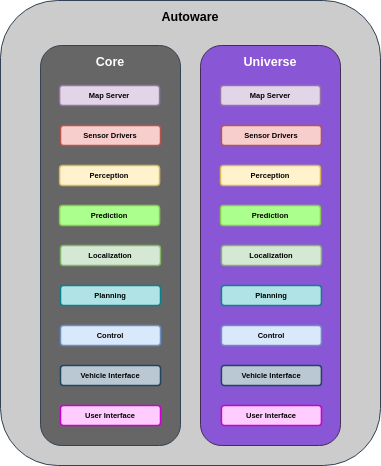
\includegraphics[width=0.5\linewidth]{figures/microautonomy_core_universe_modules.png}
    \caption{دو مدول اصلی \lr{Autoware} \cite{Autoware:Documentation}}
    \label{fig:Microautonomy_Core_Universe_Modules}
\end{figure}

\subsection{مدول \lr{Core}}
مدول \lr{Core} یا هسته، شامل برنامه‌های اجرایی‌ اساسی و مولفه‌هایی است که امکان حس کردن، محاسبه و اجرای مورد نیاز برای خودروهای خودران را فراهم می‌سازد. شرکت \lr{AWF}، مدول \lr{Core} را از طریق گروه‌های کاری خود و با معماران و اعضای برجسته‌ی خود توسعه داده و به‌روزرسانی می‌کند. هر کسی می‌تواند به مدول \lr{Core} مولفه یا کدی اضافه کند؛ اما معیارهای پذیرش این مشارکت، نسبت به مدول \lr{Universe} سخت‌گیرانه‌تر و دقیق‌تر است \cite{Autoware:Documentation}.

\subsection{مدول \lr{Universe}}
مدول‌های \lr{Universe} یا دنیا، افزونه‌هایی برای مدول \lr{Core} هستند که توسط توسعه‌دهندگان فناوری ارائه می‌شوند، تا عملکرد و توانایی حس کردن، محاسبه و اجرا را بهبود دهند. شرکت \lr{AWF}، مدول پایه \lr{Universe} را برای گسترش ارائه می‌دهد. یک ویژگی کلیدی از معماری خودمختار در ابعاد میکرو، این است که مدول‌های \lr{Universe} می‌توانند توسط مشارکت هر سازمان و فردی ساخته شوند. به عبارت دیگر، شما می‌توانید حتی مدول‌های خودتان را ایجاد کرده و برای جامعه و اکوسیستم \lr{Autoware}، در دسترس قرار دهید. شرکت \lr{AWF}، مسئول کنترل کیفیت مدول‌های \lr{Universe} در طول فرآیند توسعه آنها هستند. در نتیجه، مدول‌های \lr{Universe} دارای انواع مختلفی هستند - برخی توسط \lr{AWF} تأیید و اعتبارسنجی شده‌اند و برخی دیگر نه. انتخاب و ادغام مدول‌های \lr{Universe} برای ایجاد برنامه‌های نهایی به عهده کاربران \lr{Autoware} است. کاربران می‌توانند مولفه‌هایی از مدول \lr{Core} را با مولفه‌های \lr{Universe} که عموما بروزتر و نوین‌تر است، تعویض کنند \cite{Autoware:Documentation}.\\
\\
در ادامه، نگاهی اجمالی به مولفه‌های اصلی تشکیل‌دهنده این مدول‌ها می‌اندازیم.

\subsection{مولفه \lr{Sensing}}
مولفه \lr{Sensing} یا احساس، مجموعه‌ای از مدول‌ها است که پیش‌ پردازش‌هایی اولیه را بر روی داده‌ی ورودی از سمت حسگر‌ها، اعمال می‌کنند. ورودی‌های این مولفه در \cref{fig:Sensing_Input_Types} آمده است \cite{Autoware:Documentation}.

\begin{figure}[h!]
    \centering
    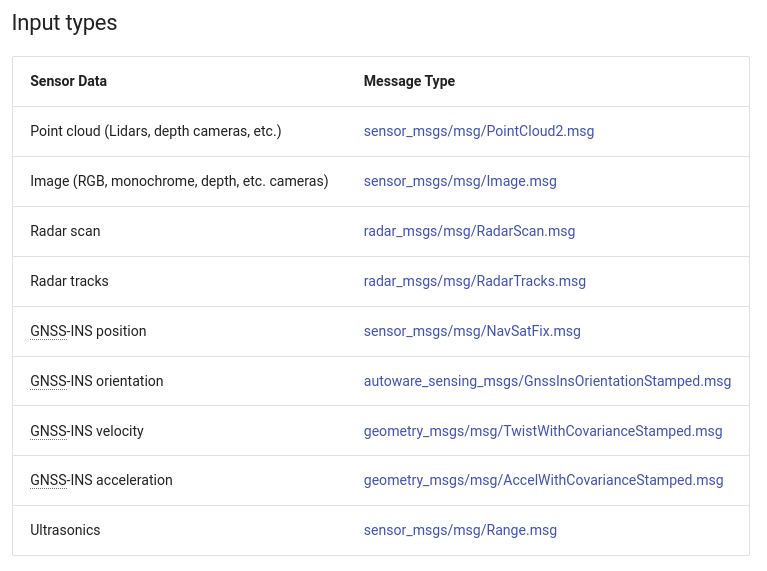
\includegraphics[width=0.64\linewidth]{figures/Sensing_Input_Types.png}
    \caption{انواع ورودی‌های قابل پذیرش توسط مولفه \lr{Sensing} \cite{Autoware:Documentation}}
    \label{fig:Sensing_Input_Types}
\end{figure}

\begin{figure}[h!]
    \centering
    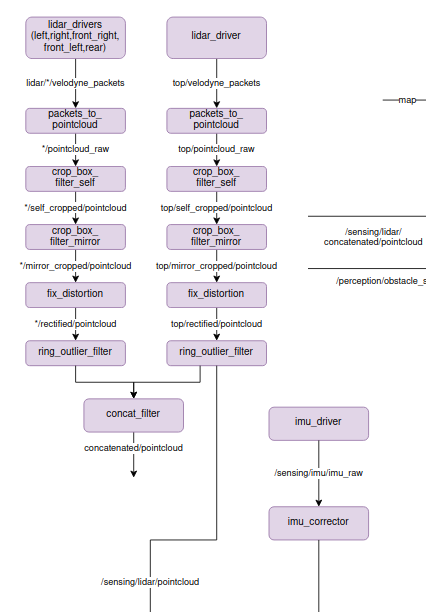
\includegraphics[width=0.75\linewidth]{figures/Sensing_Node_Graph.png}
    \caption{گراف گره‌ی مولفه ‌\lr{Sensing} \cite{Autoware:Documentation}}
    \label{fig:Sensing_Node_Graph}
\end{figure}
همانطور که در \cref{fig:Sensing_Node_Graph} مشاهده می‌شود، مبحث‌های \lr{ROS} که هر کدام از فیلتر‌های اعمال شده بر ابر‌ نقاط ورودی، به آن داده‌ منتشر ‌می‌کنند، نوشته ‌شده است\LTRfootnote{\url{https://autowarefoundation.github.io/autoware-documentation/main/design/autoware-architecture/sensing/}}.

\subsection{مولفه \lr{Map}}
نرم‌افزار \lr{Autoware}، برای انجام وظایف مختلفی نظیر موقعیت‌یابی\LTRfootnote{\lr{Localization}}، برنامه‌ریزی مسیر\LTRfootnote{\lr{Route Planning}}، تشخیص چراغ‌های راهنمایی و رانندگی، و پیش‌بینی مسیر حرکت عابر‌پیاده‌ها و دیگر وسایل نقلیه، از نقشه‌های ابر نقاط\LTRfootnote{\lr{Pointcloud Map}} با وضوح بالا و نقشه‌های برداری\LTRfootnote{\lr{Vector Map}} از محیط رانندگی، استفاده می‌کند.

مولفه \lr{Map}، بایستی دو مدل اطلاعات را برای دیگر پشته‌ها فراهم کند:
\begin{enumerate}
    \item اطلاعات معنایی\LTRfootnote{\lr{Semantic Information}} مربوط به جاده‌ها در نقشه بُرداری
    \item اطلاعات ژئومتریک\LTRfootnote{\lr{Geometric Information}} مربوط به محیط در نقشه ابر نقاط
\end{enumerate}

\begin{figure}[h!]
    \centering
    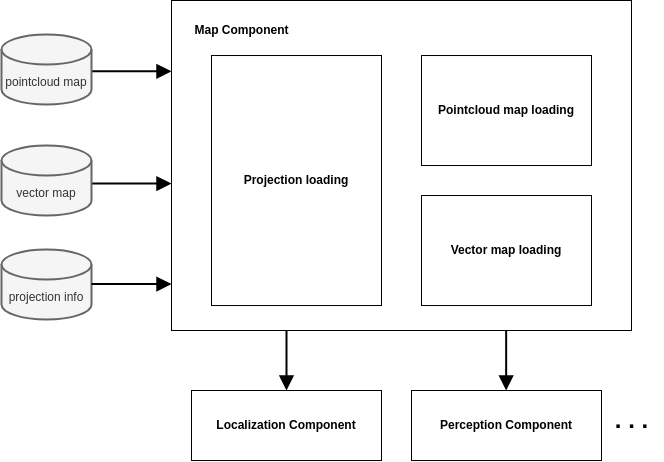
\includegraphics[width=0.75\linewidth]{figures/Autoware_Map_Architecture.png}
    \caption{معماری مولفه \lr{Map} \cite{Autoware:Documentation}}
    \label{fig:Autoware_Map_Architecture}
\end{figure}

یک نقشه بُرداری، شامل اطلاعات دقیق در مورد شبکه جاده، هندسه مسیر‌های عبوری و چراغ‌های راهنمایی و رانندگی می‌شود. این اطلاعات برای برنامه‌ریزی مسیر، تشخیص چراغ‌های راهنمایی و پیش‌بینی مسیر حرکت دیگر وسایل نقلیه و عابر‌پیاده‌ها ضروری هستند.

یک نقشه ابر نقاط سه بعدی، در درجه اول برای موقعیت‌یابی لایدار-محور و بخشی از مولفه \lr{Perception} در \lr{Autoware}، استفاده می‌شود. به منظور تعیین مکان و جهت فعلی وسیله نقلیه، اسکن زنده‌ای که از یک یا چند واحد لایدار ثبت شده است، با یک نقشه ابر نقاط سه‌بعدی پیش‌تولید شده همخوانی داده می‌شود. بنابراین، یک نقشه دقیق ابر نقاط برای نتایج خوب موقعیت‌یابی بسیار حیاتی است. با این حال، اگر وسیله نقلیه دارای یک روش موقعیت‌یابی جایگزین با دقت کافی باشد، به عنوان مثال با استفاده از موقعیت‌یابی بر اساس دوربین، احتمالاً نیازی به استفاده از نقشه ابر نقاط برای وجود نخواهد داشت \cite{Autoware:Documentation}. در \cref{fig:Autoware_Map_Architecture}، معماری‌ سطح‌ بالایی از مولفه \lr{Map} را مشاهده می‌کنیم  \LTRfootnote{\url{https://autowarefoundation.github.io/autoware-documentation/main/design/autoware-architecture/map/}}.

\begin{figure}[h!]
    \centering
    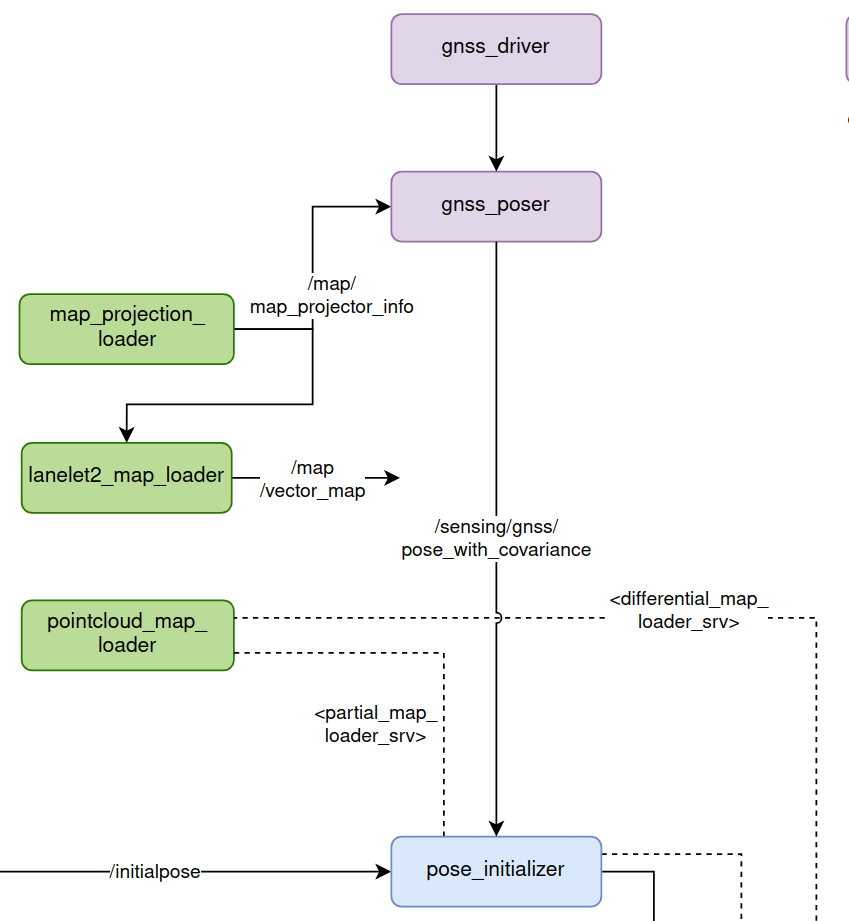
\includegraphics[width=0.75\linewidth]{figures/Autoware_Map_Node_Graph.png}
    \caption{گراف گره‌ی مولفه \lr{Map} (مستطیل‌های سبز) \cite{Autoware:Documentation}}
    \label{fig:Autoware_Map_Node_Graph}
\end{figure}

\subsection{مولفه \lr{Localization}}
مولفه \lr{Localitzation} یا موقعیت‌یابی، سعی در تخمین موقعیت، سرعت و شتاب خودروی خودران دارد. همچنین سعی شده است تا سیستمی طراحی شود که عملیات موقعیت‌یابی را با حسگر‌های مختلف انجام دهد و در صورتی که تخمین با خطای زیادی مواجه باشد، پیام هشداری را به سیستم نظارتی خودروی خودران ارسال کند.
این مولفه، با پیکربندی حسگر‌های مختلف زیر کار می‌کند:
\begin{enumerate}
    \item لایدار سه‌بعدی + نقشه ابر نقاط
    \item لایدار سه‌بعدی یا دوربین + نقشه بُرداری
    \item  دوربین (ادومتری بصری،‌ محلی‌سازی و نقشه‌برداری همزمان\LTRfootnote{\lr{SLAM: Simultaneous Localization And Mapping}} بصری)
    \item حسگر سرعت چرخ
    \item واحد اندازه‌گیری لختی \LTRfootnote{\lr{IMU: Inertial Measurement Unit}}
    \item حسگر ژئو-مغناطیسی\LTRfootnote{\lr{Geomagnetic Sensor}}
    \item نشانگرهای مغناطیسی\LTRfootnote{\lr{Magnetic Markers}}
\end{enumerate}

در \cref{fig:Autoware_Localization_Architecture}، معماری‌ پیشنهادی، که توسط توسعه‌دهندگان \lr{Autoware} برای توسعه‌دهندگان دیگر در اختیار گذاشته‌اند، مشاهده می‌شود. برای دقت بالا در موقعیت یابی، پیشنهاد شده است که واحد اندازه‌گیری لختی و حسگر لایدار حتما استفاده شوند؛ همچنین نقشه بُرداری و نقشه ابر نقاط محیط نیز به عنوان ورودی به مولفه \lr{Localization} داده شوند \cite{Autoware:Documentation}.

\begin{figure}[h!]
    \centering
    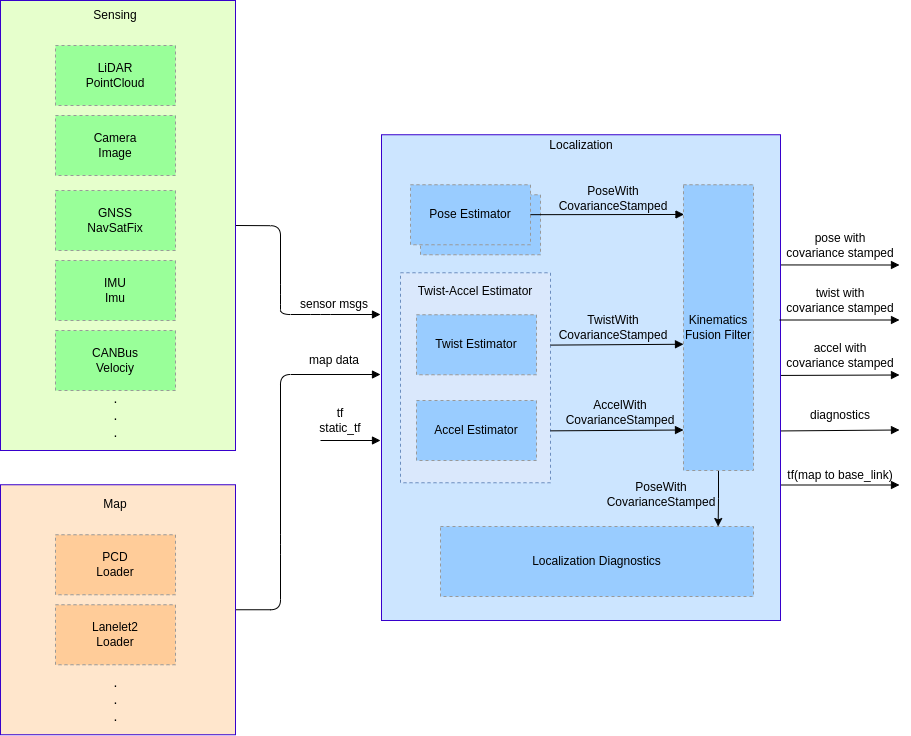
\includegraphics[width=0.75\linewidth]{figures/Autoware_Localization_Architecture.png}
    \caption{معماری پیشنهادی \lr{Autoware} برای مولفه \lr{Localization} \cite{Autoware:Documentation}}
    \label{fig:Autoware_Localization_Architecture}
\end{figure}

\begin{figure}[h!]
    \centering
    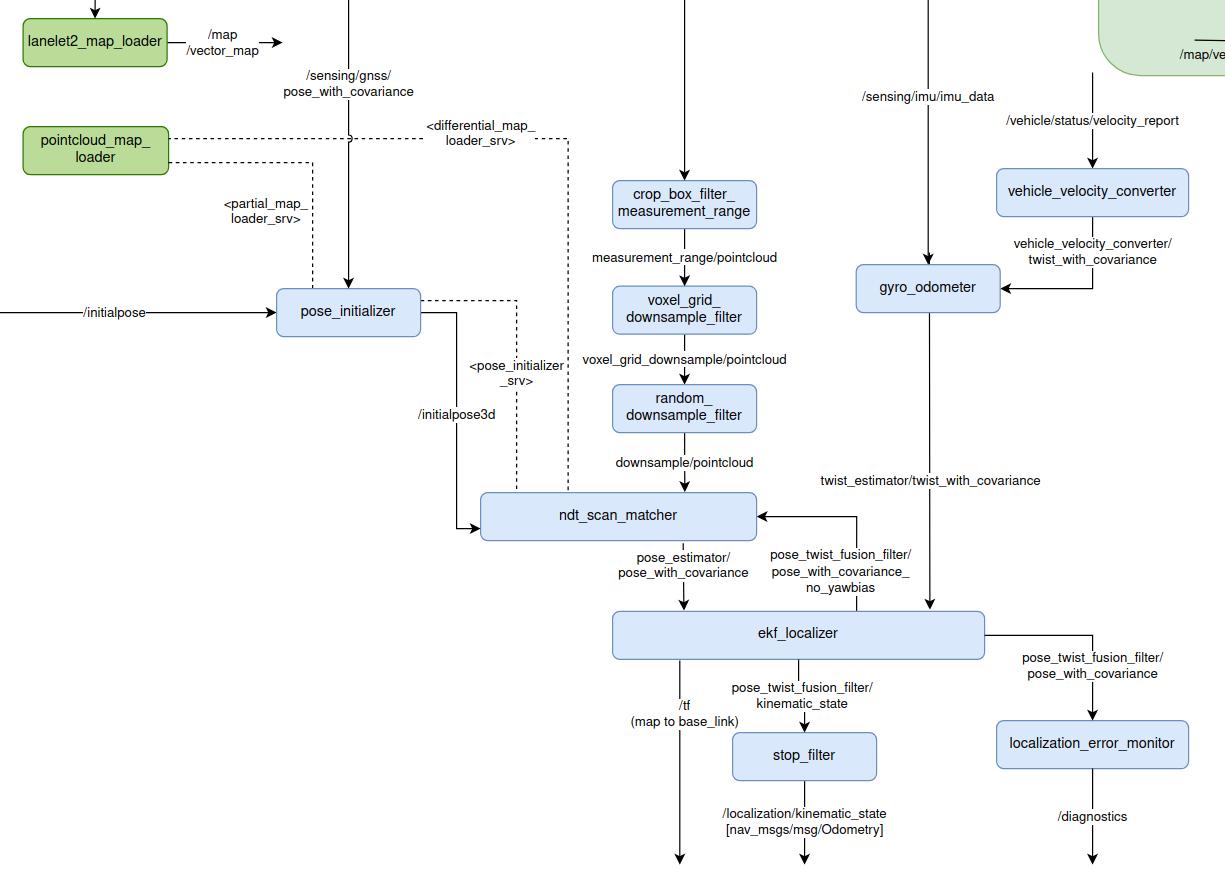
\includegraphics[width=0.85\linewidth]{figures/Autoware_Localization_Node_Graph.png}
    \caption{گراف گره‌ی مولفه \lr{Localization} \cite{Autoware:Documentation}}
    \label{fig:Autoware_Localization_Node_Graph}
\end{figure}

\subsection{مولفه \lr{Perception}}
مولفه \lr{Perception} یا ادراک، وظیفه‌ی تشخیص انواع وسایل نقیه مانند خودرو، کامیون، موتور، اتوبوس، و همچنین عابرین پیاده را بر عهده دارد. این مولفه، علاوه بر تشخیص اجسام سه‌بعدی ذکر شده، شناسه‌ی یکتایی را به آنها نسبت می‌دهد و آنها را ردیابی\LTRfootnote{\lr{Track}}  می‌کند تا موقعیت، شتاب، سرعت، مسیر حرکت و جهت قرارگیری آنها را محاسبه کند. این مولفه در مدول \lr{Universe} دارای الگوریتم‌های گوناگونی برای ادراک محیط است و ورودی‌های آن همانند مولفه \lr{Sensing} می‌باشد. این مولفه از چند گره اصلی تشکیل شده است:
\begin{enumerate}
    \item گره‌ پیش‌پردازش
    \item گره تشخیص  و ردیابی اجسام سه‌بعدی
    \item گره تشخیص علایم راهنمایی و رانندگی
    \item گره پیش‌بینی مسیر حرکت اجسام
    \item گره پس‌پردازش
\end{enumerate}

بایستی توجه داشت که ورودی‌های ابر نقاط لایدار، برای این مولفه ضروری است و نداشتن آن، دقت تشخیص را به مراتب کاهش می‌دهد. در معماری رابط‌های مولفه \lr{Perception}، مشاهده می‌شود. همانطور که ذکر شد، پیشنهاد می‌شود که حتما از داده‌های ابر نقاط برای تشخیص اجسام استفاده کرد.

\begin{figure}[h!]
    \centering
    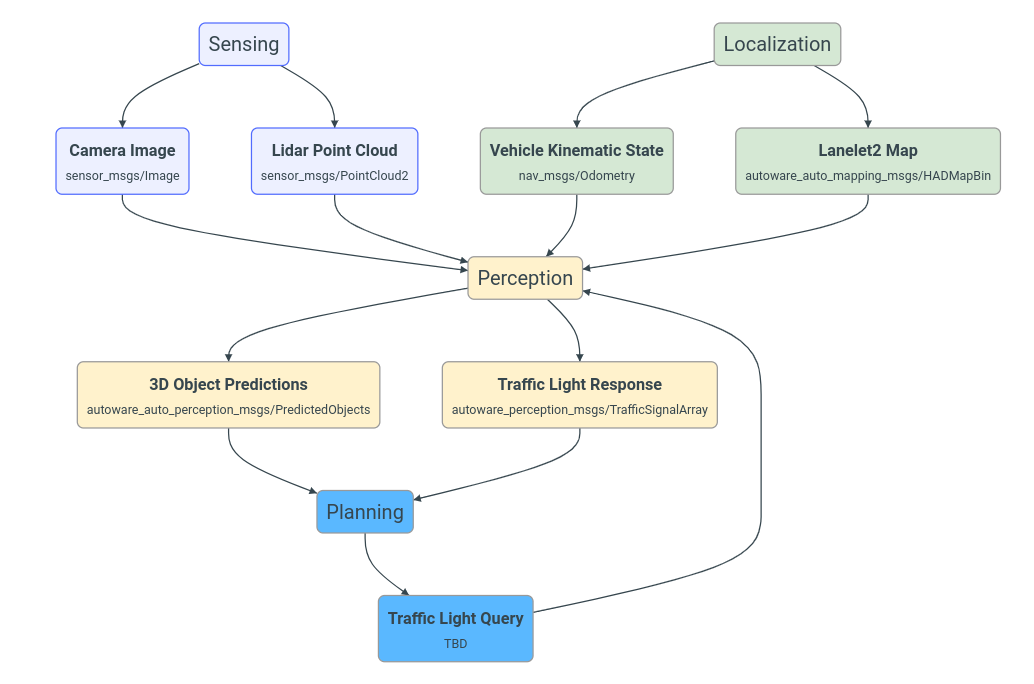
\includegraphics[width=0.85\linewidth]{Autoware_Perception_Interface_Architecture.png}
    \caption{معماری رابط‌های مولفه \lr{Perception} \cite{Autoware:Documentation}}
    \label{fig:Autoware_Perception_Interface_Architecture}
\end{figure}

از آنجایی که در این پژوهش، از این مولفه استفاده شده است، لازم است تا برخی از گره‌های مهم آن توضیح داده شوند.

\subsubsection{گره پیش‌پردازش}
این گره وظیفه اعمال فیلترهایی اولیه به ابر نقاط ورودی را بر عهده دارد. 

\begin{figure}[h!]
    \centering
    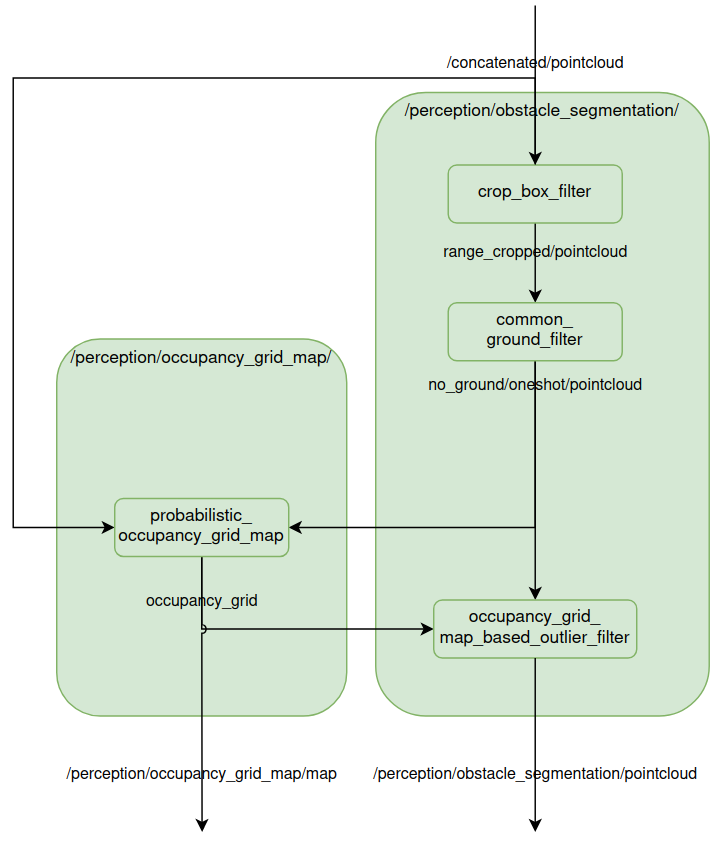
\includegraphics[width=0.45\linewidth]{figures/Autoware_Perception_Preprocessing_Node_Graph.png}
    \caption{ گراف گره‌ی پیش‌پردازش مولفه \lr{Perception} \cite{Autoware:Documentation}}
\label{fig:Autoware_Perception_Preprocessing_Node_Graph}
\end{figure}

طبق \cref{fig:Autoware_Perception_Preprocessing_Node_Graph} مشاهده می‌کنیم که گره پیش‌پردازش، خود از گره‌هایی کوچک‌تر ساخته شده‌اند که عبارتند از:
\begin{enumerate}
    \item فیلتر \lr{crop\_box}: این گره با استفاده از کتابخانه \lr{PCL}\LTRfootnote{\lr{Point Cloud Library} : \url{https://pcl.readthedocs.io/projects/tutorials/en/master/\#}} تمام نقاطی که در یک منطقه مکعبی مشخص شده باشد را از ابر نقاط حذف می‌کند. از این گره برای فیلتر کردن نقاطی که مربوط به خود خودروی  خودران است، استفاده می‌شود.
    \item فیلتر \lr{common\_ground}:‌ این گره برای حذف نقاط زمین از ابر نقاط استفاده می‌کند\LTRfootnote{\url{https://autowarefoundation.github.io/autoware.universe/main/perception/ground_segmentation/}}. 
    \item نقشه شبکه اشغال احتمالاتی\LTRfootnote{\lr{Probabilistic Occupancy Grid Map}}: از این گره برای ساختن نقشه‌ای از احتمال وجود موانع در اطراف ماشین خودران، استفاده می‌شود\LTRfootnote{\url{https://autowarefoundation.github.io/autoware.universe/main/perception/probabilistic_occupancy_grid_map/}}.
\end{enumerate}

\subsubsection{گره تشخیص و ردیابی اجسام سه‌بعدی}
در این گره که همانند گره پیش‌پردازش از چندین گره کوچکتر ساخته شده است، ابر نقاط فیلتر شده به عنوان ورودی به مدل‌ تشخیص‌دهنده اجسام سه‌بعدی داده می‌شود و سپس بر روی کادر محصور‌کننده خروجی این مدل، الگوریتم‌های ردیابی زده می‌شود. در \cref{fig:Autoware_Perception_Detection_Node_Graph} معماری گره تشخیص مشاهده می‌شود. همانطور که از شکل معلوم است، گره \lr{Perception} از گره‌های کوچکتری تشکیل شده است که عبارتند از:
\begin{enumerate}
    \item گره تشخیص دهنده سه‌بعدی \lr{(lidar\_centerpoint)}: این گره، یک مدل هوش مصنوعی تشخیص سه‌بعدی ابر نقاط-محور مبتنی بر واکسل، به نام \lr{Centerpoint} است \cite{yin2021center}. ابر نقاط فیلتر شده به عنوان ورودی به این تشخیص دهنده داده‌ می‌شود و کادر‌های محصور کننده اجسام تشخیص داده شده، به عنوان خروجی دریافت می‌شوند. این مدل هوش مصنوعی، از یک شبکه عصبی بر مبنای \lr{PointPillars} \cite{lang2019pointpillars} استفاده می‌کند. این شبکه عصبی با بهره‌وری از کتابخانه \lr{TensorRT}\LTRfootnote{\url{https://developer.nvidia.com/tensorrt}}، که برای سرعت‌های بسیار بالا (تشخیص بلادرنگ) و استفاده بهینه از کارت گرافیکی ساخته شده است، پیاده‌سازی شده است.
    \item گره اعتبار سنجی موانع براساس ابر نقاط \lr{(obstacle\_pointcloud\_based\_validator)}: این گره، خروجی مدل هوش‌ مصنوعی را بررسی می‌کند و اجسامی که از مجموعه نقاط کمی تشکیل شده باشند را به عنوان مثبت‌های کاذب تشخیص داده و حذف می‌کند.
    \begin{figure}[h!]
    \centering
    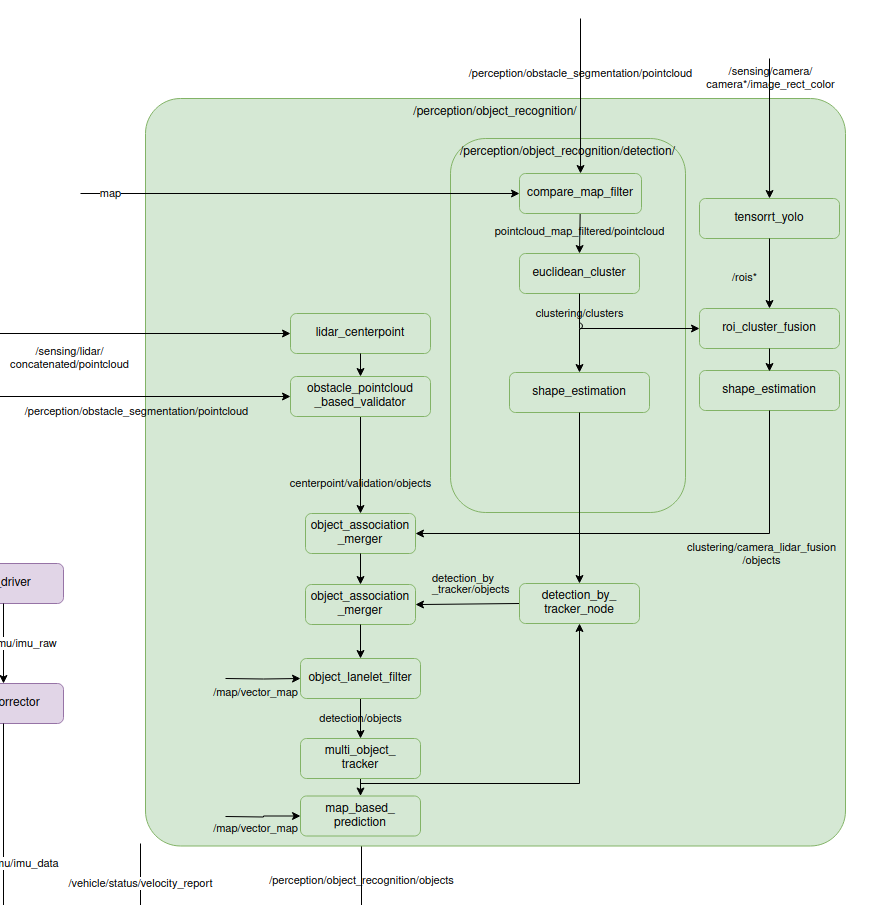
\includegraphics[width=1\linewidth]{figures/Autoware_Perception_Detection_Node_Graph.png}
    \caption{گراف گره‌‌ی تشخیص اجسام و ردیابی مولفه \lr{Perception} \cite{Autoware:Documentation}}
    \label{fig:Autoware_Perception_Detection_Node_Graph}
    \end{figure}
    \item گره فیلتر مقایسه نقشه \lr{(compare\_map\_filter)}: این گره برای تشخیص نقاط مربوط به زمین و حذف آن‌ها با استفاده از نقشه ابر نقاط است\LTRfootnote{\url{https://autowarefoundation.github.io/autoware.universe/main/perception/compare_map_segmentation/}}.
    \item گره خوشه‌بندی اقلیدسی \lr{(euclidean\_cluster)}: این گره، با استفاده از خوشه‌بندی اقلیدسی کتابخانه \lr{PCL}، اقدام به خوشه‌بندی ابر نقاط می‌کند که از آن برای تشخیص اجسام و همچنین تشخیص ابعاد اجسام استفاده می‌شود\LTRfootnote{\url{https://autowarefoundation.github.io/autoware.universe/main/perception/euclidean_cluster/}}.
    \item گره تخمین شکل \lr{(shape\_estimation)}: این گره، شکل دقیق‌تری از جسم (کادر محصورکننده \cite{Zhang-2017-26536}، استوانه، پوشش محدب\LTRfootnote{\lr{Convex Hull}}) را که خوشه‌ی ابر نقاط در ارتباط با یک برچسب، در آن جا می‌شود را محاسبه می‌کند.
    \item گره ادغام کننده اجسام \lr{(object\_association\_merger)}: این گره اجسام تشخیص داده‌ شده از دو روش تشخیص اجسام مختلف را ادغام می‌کند\LTRfootnote{\url{https://autowarefoundation.github.io/autoware.universe/main/perception/object_merger/}}.
    \item گره فیلتر لینلت \lr{(object\_lanelet\_filter)}: این گره، اجسام تشخیص داده شده را براساس نقشه بُرداری فیلتر می‌کند. این گره تنها اجسامی که داخل خطوط جاده‌ها و پیاده‌رو‌ها باشند را از فیلتر عبور می‌دهد\LTRfootnote{\url{https://autowarefoundation.github.io/autoware.universe/main/perception/detected_object_validation/object-lanelet-filter/}}.
    \item گره ردیاب هم‌زمان چند جسم \lr{(multi\_object\_tracker)}: نتایج تشخیص اجسام، توسط یک سری زمانی پردازش می‌شوند. هدف اصلی، دادن شناسه یکتا به هر یک از اجسام تشخیص داده شده و تخمین سرعت ‌آن‌ها است\LTRfootnote{\url{https://autowarefoundation.github.io/autoware.universe/main/perception/multi_object_tracker/}}.
    \item گره تشخیص براساس ردیاب \lr{(detection\_by\_tracker)}: این گره، اجسام ردیابی شده را به گره تشخیص باز می‌گرداند تا پایدار بماند و به شناسایی اجسام ادامه دهد. این گره یک جسم ناشناخته حاوی یک خوشه نقاط و یک ردیاب را به عنوان ورودی، دریافت می‌کند. جسم ناشناخته تا مرحله متناسب شدن با ابعاد ردیاب، بهینه ‌می‌شود تا بتواند به شناسایی شدن ادامه دهد. 
    گره‌ی تشخیص با استفاده از ردیاب، یک شئ ناشناخته شامل یک ابر نقطه و یک ردیاب دریافت می‌کند، سپس شکل شیء ناشناخته با استفاده از خوشه‌بندی اقلیدسی، متناسب می‌شود. متناسب‌سازی شکل با استفاده از خوشه‌بندی اقلیدسی و روش‌های دیگر مشکلی به نام کم‌تقسیم‌بندی\LTRfootnote{\lr{Under-Segmentation}} و بیش‌تقسیم‌بندی\LTRfootnote{\lr{Over-Segmentation}} دارد، که با اعمال سیاست‌هایی بهبود می‌یابد\LTRfootnote{\url{https://autowarefoundation.github.io/autoware.universe/main/perception/detection_by_tracker/}} \cite{Autoware_Universe:Documentation}.
\end{enumerate}

\subsection{مولفه \lr{Planning}}
مولفه \lr{Planning} یا برنامه‌ریزی مسیر، پیام مسیر پیشنهادی را براساس وضعیت محیط که از مولفه‌های ادراک و موقعیت‌یابی بدست می‌آورد، منتشر می‌کند و مولفه \lr{Control} از این پیام استفاده می‌کند.

\begin{figure}[h!]
    \centering
    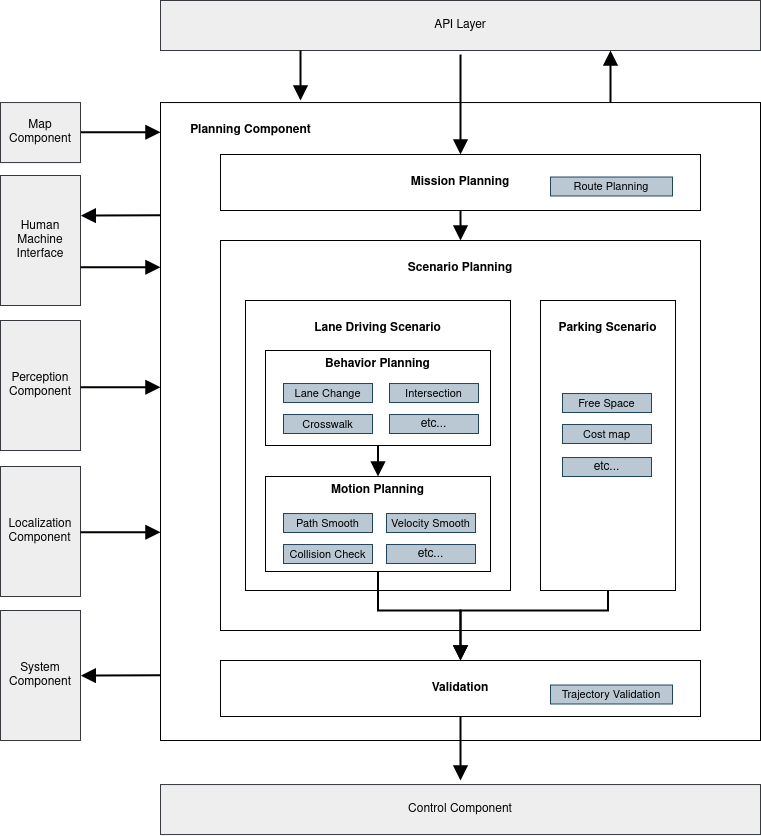
\includegraphics[width=0.75\linewidth]{figures/Autoware_Planning_Architecture.png}
    \caption{معماری سطح بالای مولفه \lr{Planning} \cite{Autoware:Documentation}}
    \label{fig:Autoware_Planning_Architecture}
\end{figure}

همانطور که طبق \cref{fig:Autoware_Planning_Architecture} مشاهده می‌شود، مولفه \lr{Planning} از چند مولفه کوچک‌تر ساخته شده است:
\begin{enumerate}
    \item مولفه برنامه‌ریزی ماموریت \lr{(Mission Planning)}:‌ مسیر را براساس هدف و اطلاعات نقشه  داده شده، محاسبه می‌کند.
    \item مولفه برنامه‌ریزی سناریو \lr{(Scenario Planning)}: مسیر را براساس سناریو حال حاضر تعیین می‌کند (به طور مثال سناریو رانندگی در خطوط جاده یا سناریو پارک کردن).
    \begin{itemize}
        \item مولفه رانندگی در خطوط \lr{(Lane Driving)}: مسیر را برای رانندگی در بین خطوط جاده را محاسبه می‌کند.
        \item مولفه برنامه‌ریزی رفتار \lr{(Behavior Planner)}: مسیر مطلوب را براساس ملاحظات ایمنی و قوانین راهنمایی رانندگی، محسابه می‌کند.
        \item مولفه برنامه‌ریزی حرکت \lr{(Motion Planner)}: مسیر مطلوب خودرو را براساس عامل‌های ایمنی، ملاحظات سرعت خودرو و دستورات مولفه برنامه‌ریزی رفتار، محسابه می‌کند.
        \item مولفه پارک کردن \lr{(Parking)}: مسیر را در سناریوهای پارک کردن در جای ناشناخته، محاسبه می‌کند.
    \end{itemize}
    \item مولفه اعتبارسنجی \lr{(Validation)}: ایمن بودن مسیر محاسبه شده را می‌سنجد.
\end{enumerate}

هر کدام از مولفه‌ها می‌توانند براساس وضعیت، به صورت پویا اضافه و حذف شوند. این معماری، برگرفته از معماری خودمختار در ابعاد میکرو نرم‌افزار \lr{Autoware} است، که این اجازه را می‌دهد که هر کدام از مولفه‌ها نسبت به شرایط، به خط‌ لوله اجرایی اضافه یا از آن حذف شوند \cite{Autoware:Documentation}. 

برای مشاهده گراف گره این مولفه، می‌توان به صفحه گراف گره کلی \lr{Autoware} مراجعه کرد\LTRfootnote{\url{https://autowarefoundation.github.io/autoware-documentation/main/design/autoware-architecture/node-diagram/}}. همچنین دو مولفه پایانی \lr{Control} و \lr{Vehicle}، به علت مربوط نبودن به پژوهش، توضیح داده نمی‌شوند. \cref{fig:Autoware_Architecture}،‌ معماری کلی نرم‌افزار \lr{Autoware} را در یک نگاه نشان می‌دهد.

\begin{figure}[h!]
    \centering
    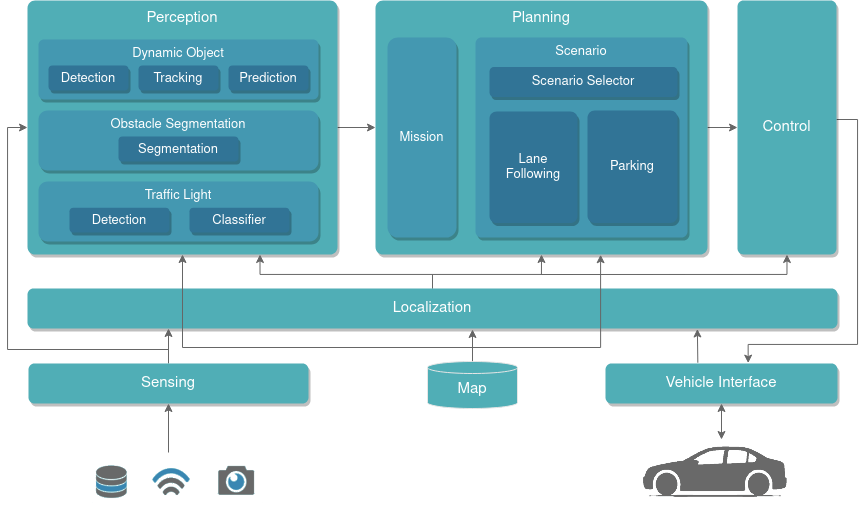
\includegraphics[width=1\linewidth]{figures/Autoware_Architecture.png}
    \caption{معماری سطح‌‌بالای نرم‌افزار \lr{Autoware} \cite{Autoware:Documentation}}
    \label{fig:Autoware_Architecture}
\end{figure}

\section{شبیه‌ساز \lr{AWSIM}}
\begin{figure}[h!]
    \centering
    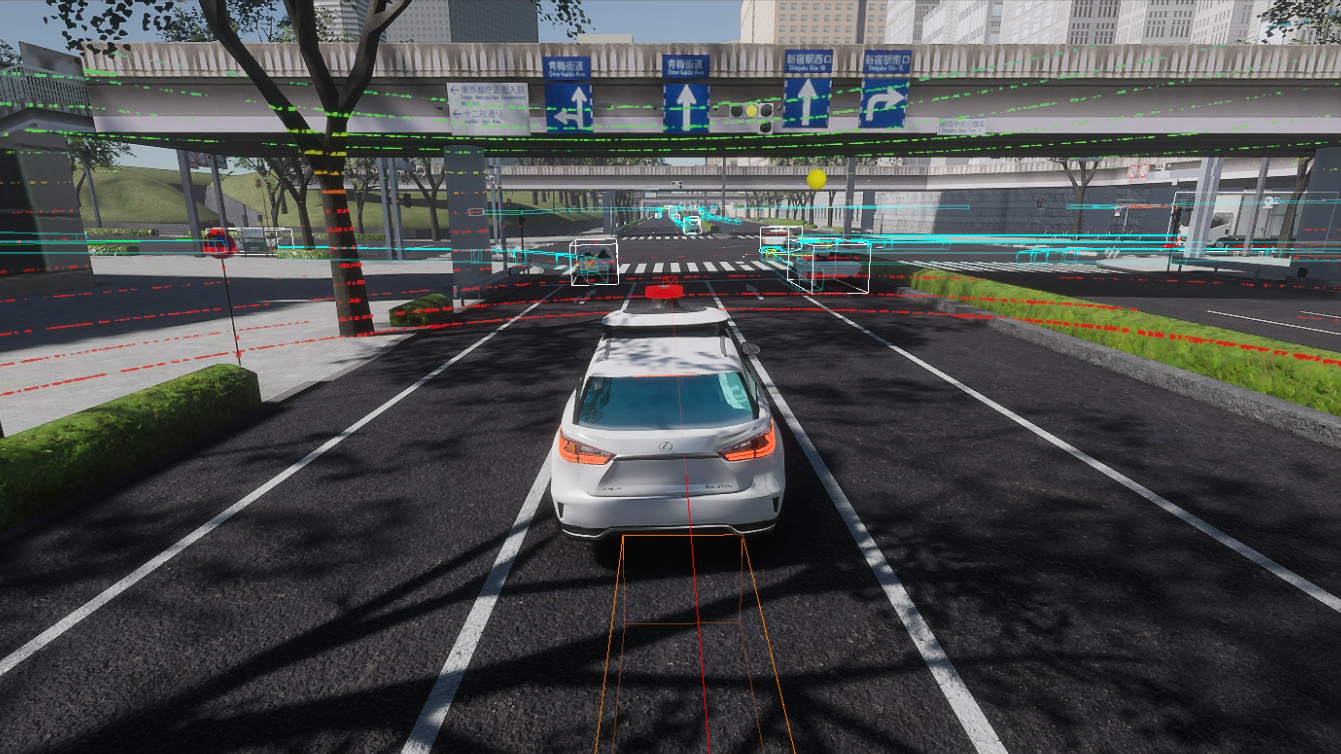
\includegraphics[width=1\linewidth]{figures/E2ESim.png}
    \caption{شبیه‌ساز \lr{AWSIM} \cite{AWSIM:Documentation}}
    \label{fig:AWSIM}
\end{figure}

\lr{AWSIM} یک شبیه‌ساز متن‌باز ساخته شده با استفاده از موتور بازی‌سازی \lr{Unity} است که برای تحقیق و توسعه در حوزه رانندگی خودکار است. این شبیه‌ساز برای نرم‌افزارهای خودروی خودران همانند \lr{Autoware}، ساخته شده است. هدف این شبیه‌ساز، ایجاد ارتباط بین دنیای مجازی و واقعی است، به طوری که به کاربران اجازه می‌دهد تا سیستم‌های خودران خود را قبل از اینکه بر روی خودروهای واقعی مستقر کنند؛ در یک محیط ایمن و کنترل‌شده، آموزش دهند و ارزیابی کنند. این شبیه‌ساز محیط مجازی واقع‌گرا، برای آموزش، آزمایش و ارزیابی جوانب مختلفی از سیستم‌های رانندگی خودکار ارائه می‌دهد.

\lr{AWSIM} سناریوهای واقعی متنوعی را با مدل‌های دقیق فیزیک و حسگر، شبیه‌سازی می‌کند. این شبیه‌ساز دارای مجموعه‌ گسترده‌ای از حسگرها مانند دوربین‌ها، لایدارها،‌ واحد اندازه‌گیری لختی و سیستم ناوبری جهانی ماهواره مبنا\LTRfootnote{\lr{Global Navigation Satellite System (GNSS)}} می‌باشد که به توسعه‌دهندگان اجازه می‌دهد تا تعاملات وسیله نقلیه خودران خود را با محیط به صورت دقیق شبیه‌سازی کنند. این شبیه‌ساز همچنین اشیاء پویا مانند عابرین پیاده، دیگر وسایل نقلیه و چراغ‌های راهنمایی رانندگی را نیز مدل‌سازی می‌کند، که امکان مطالعه تعاملات و تصمیم‌گیری در سناریوهای پیچیده ترافیکی را فراهم می‌کند. این موضوع، امکان آزمون و ارزیابی الگوریتم‌های ادراک، برنامه‌ریزی و کنترل در پیکربندی‌های مختلف حسگرها و سناریوها را می‌دهد.

\lr{AWSIM}، از یک معماری انعطاف پذیر و مدولار\LTRfootnote{\lr{Modular}} پشتیبانی می‌کند، که امکان تغییر و گسترش قابلیت‌های آن را آسان می‌کند. کاربران می‌توانند محیط\LTRfootnote{\lr{Environment}} فعلی شبیه‌ساز را تغییر دهند یا محیط جدیدی با عناصر\LTRfootnote{\lr{Assets}} و قوانین ترافیک خود اضافه کنند، تا سناریوهای خاص خود را برای تحقیقاتشان ایجاد کنند \cite{AWSIM:Documentation}. 

\subsection{معماری}

\begin{figure}[h!]
    \centering
    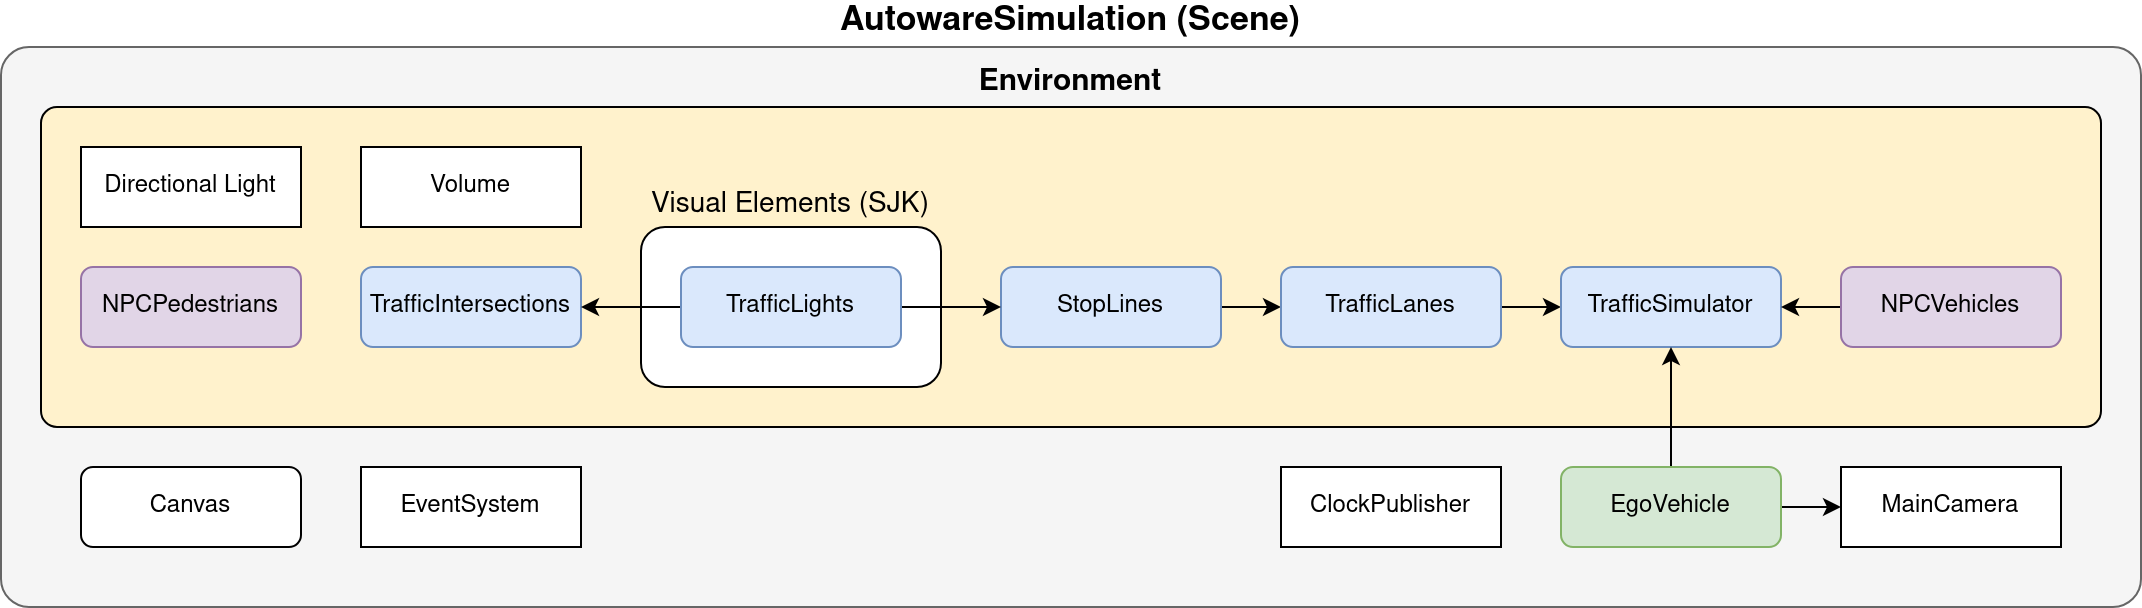
\includegraphics[width=1\linewidth]{figures/AWSIM_Architecture.png}
    \caption{معماری سطح بالای شبیه‌ساز \lr{AWSIM} \cite{AWSIM:Documentation}}
    \label{fig:AWSIM_Architecture}
\end{figure}

برای توصیف معماری \lr{AWSIM}، ابتدا باید به صحنه\LTRfootnote{\lr{Scene}} بازی اشاره کرد. این صحنه، تمام اشیاء موجود در شبیه‌سازی یک سناریو خاص و تنظیمات آن‌ها را شامل می‌شود. صحنه پیش‌فرض \lr{AWSIM} که برای کار با \lr{Autoware} توسعه یافته است، به نام \lr{AutowareSimulation} شناخته می‌شود.
در این صحنه می‌توان اجزاء اساسی مانند دوربین اصلی \lr{(MainCamera)}، انتشارکننده زمان \lr{(ClockPublisher)}، سیستم رویداد \lr{(EventSystem)} و کانواس \lr{(Canvas)} را مشاهده کرد. توضیحات دقیق در مورد صحنه و اجزای آن را می‌توان در صفحه توضیحات \lr{AWSIM} خواند\LTRfootnote{\url{https://tier4.github.io/AWSIM/ProjectGuide/Scenes/}}.
علاوه بر موارد ذکرشده، این صحنه دارای دو مؤلفه دیگر بسیار مهم و پیچیده به نام‌های محیط \lr{(Environment)} و خودروی خودران \lr{(EgoVehicle)} است. حال به توضیح هر کدام می‌پردازیم \cite{Autoware:Documentation}.

\subsection{مولفه محیط}
محیط، یک مؤلفه مهم است که تمام عناصر بصری\LTRfootnote{\lr{Visual Elements}} را که محیط را در صحنه شبیه‌سازی می‌کنند و همچنین کنترل بر روی آن‌ها فراهم می‌کنند را شامل می‌شود. این مؤلفه شامل دو زیر‌مؤلفه‌ی \lr{Light} و \lr{Volume} نیز می‌شود که به تأمین نور مناسب برای عناصر بصری و شبیه‌سازی شرایط آب و هوا می‌پردازند\LTRfootnote{\url{https://tier4.github.io/AWSIM/Components/Environment/AddNewEnvironment/AddEnvironment/\#create-an-environment-prefab}}.
علاوه بر عناصر بصری مانند ساختمان‌ها و برگ‌ها، این مؤلفه شامل کلیه ساختار مربوط به ترافیک نیز می‌شود. ترافیک شامل وسایل نقلیه غیرقابل کنترل \lr{(NPCVehicles)} می‌شود که توسط مولفه شبیه‌ساز ترافیک \lr{(TrafficSimulator)} در شبیه‌سازی ایجاد می‌شوند و از مولفه‌های مرتبط با ترافیک استفاده می‌کنند\LTRfootnote{\url{https://tier4.github.io/AWSIM/Components/Traffic/TrafficComponents/}}.
عناصر \lr{NPCPedestrians} نیز جزو مؤلفه‌های محیط به حساب می‌آیند، اما توسط مولفه شبیه‌ساز ترافیک کنترل نمی‌شوند. برای حرکت آن‌ها از کد‌هایی مخصوص استفاده می‌شود\LTRfootnote{\url{https://tier4.github.io/AWSIM/Components/Traffic/NPCs/Pedestrian/}}.
\begin{figure}[h!]
    \centering
    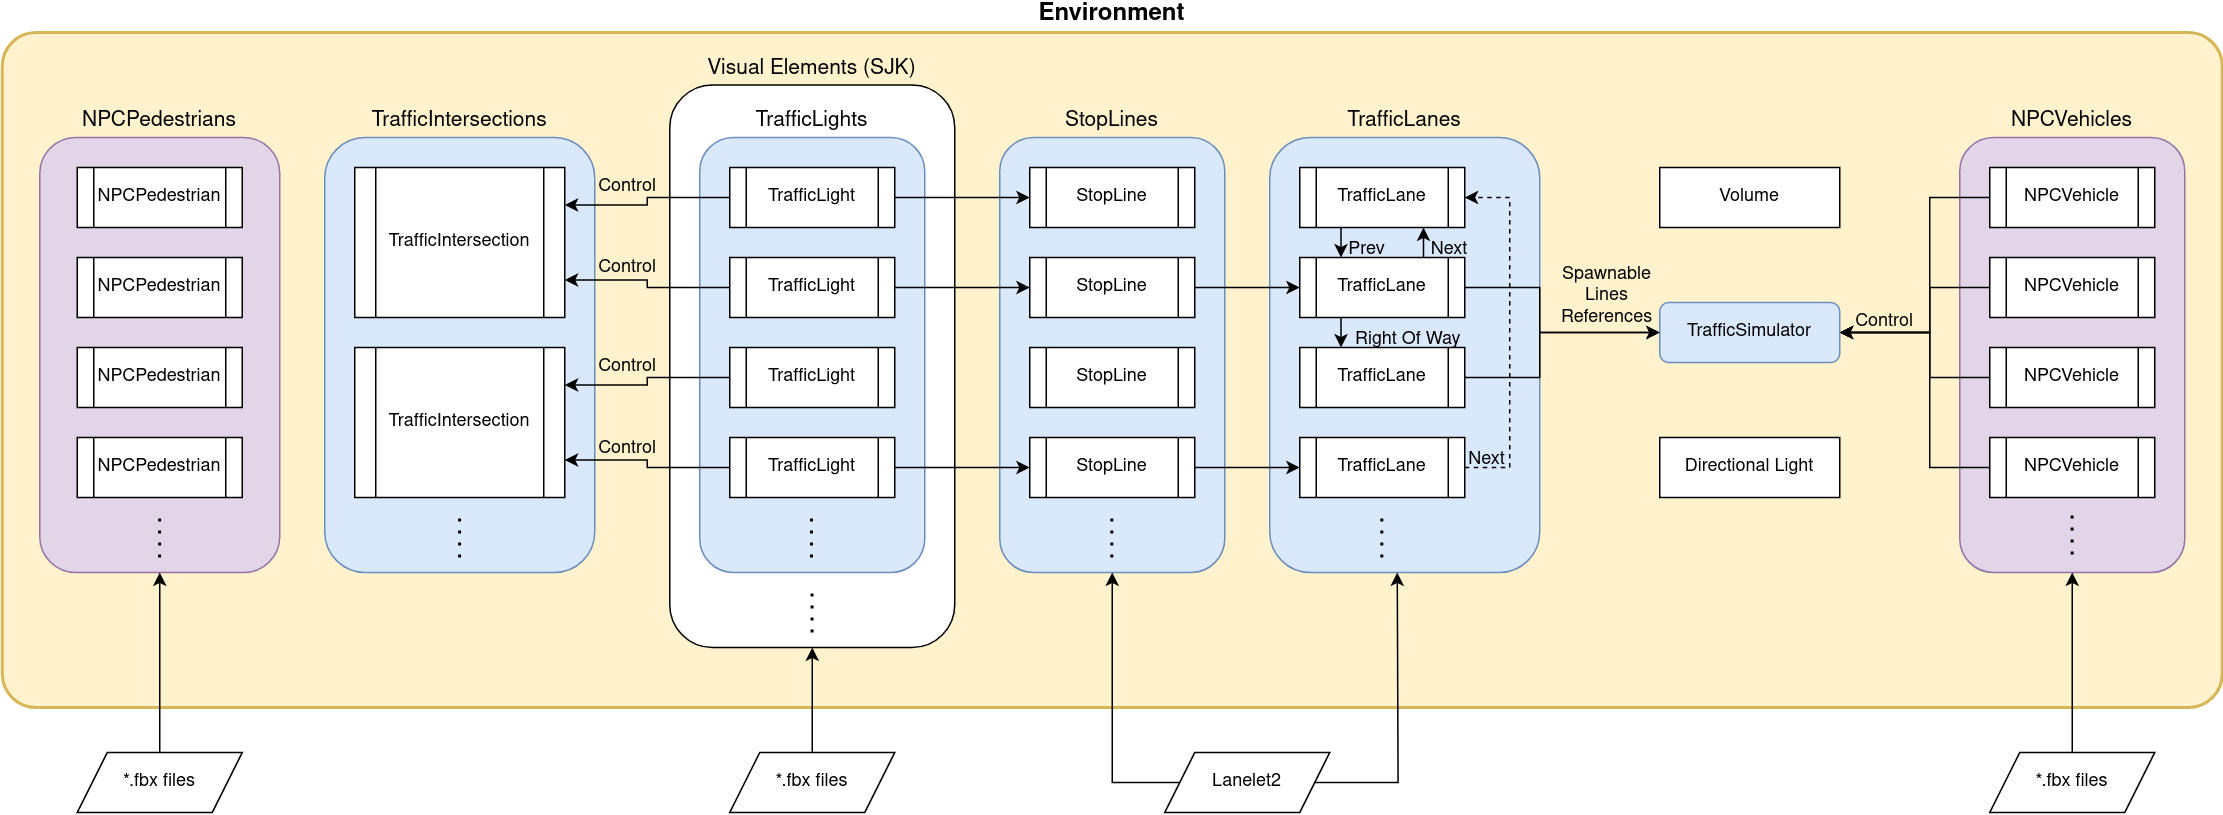
\includegraphics[width=1\linewidth]{figures/AWSIM_Environment_Architecture.png}
    \caption{معماری مولفه محیط شبیه‌ساز \lr{AWSIM} \cite{AWSIM:Documentation}}
    \label{fig:AWSIM_Environment_Architecture}
\end{figure}

\subsubsection{مولفه‌های ترافیک \lr{(Traffic)}}
مولفه‌های خطوط ترافیک \lr{(TrafficLanes)}  و خطوط ایست \lr{(StopLines)}،  عناصری هستند که از \lr{Lanelet2} (نرم‌افزار ساختن نقشه بُرداری) به محیط اضافه می‌شوند. خطوط ترافیک به گونه‌ای مراجعه متقابل\LTRfootnote{\lr{Cross-Reference}} دارند تا مسیرهایی را در محیط \lr{Unity} بر روی خطوط ترافیک ایجاد کنند. همچنین، هر خط ترافیک موجود در تقاطع\LTRfootnote{\lr{Intersection}}، شرایط خاصی برای اعطای حق تقدم دارد. مولفه شبیه‌ساز ترافیک، از مولفه خطوط ترافیک برای ایجاد \lr{NPCVehicles} و تضمین حرکت آن‌ها در امتداد این خطوط استفاده می‌کند. اگر برخی از خطوط ترافیک همچنان پیش از تقاطع به پایان برسند، دارای ارجاعی به خط ایست روبروی خود می‌باشند. هر خط ایست در تقاطع، دارای ارجاع به نزدیک‌ترین چراغ راهنمایی رانندگی \lr{(TrafficLight)} می‌باشد. چراغ‌های راهنمایی رانندگی به یکی از گروه‌های عناصر بصری تعلق دارند و رابطی برای کنترل عناصر بصری که منابع چراغ‌های ترافیکی (لامپ‌ها) را شبیه‌سازی می‌کنند، فراهم می‌کنند. یک مولفه تقاطع ترافیکی \lr{(TrafficIntersection)}، به تنهایی مسئول کنترل تمام چراغ‌های راهنمایی رانندگی در یک تقاطع است\LTRfootnote{\url{https://tier4.github.io/AWSIM/Components/Traffic/TrafficComponents/}} \cite{AWSIM:Documentation}.

\subsection{مولفه خودروی خودران}
\begin{figure}[h!]
    \centering
    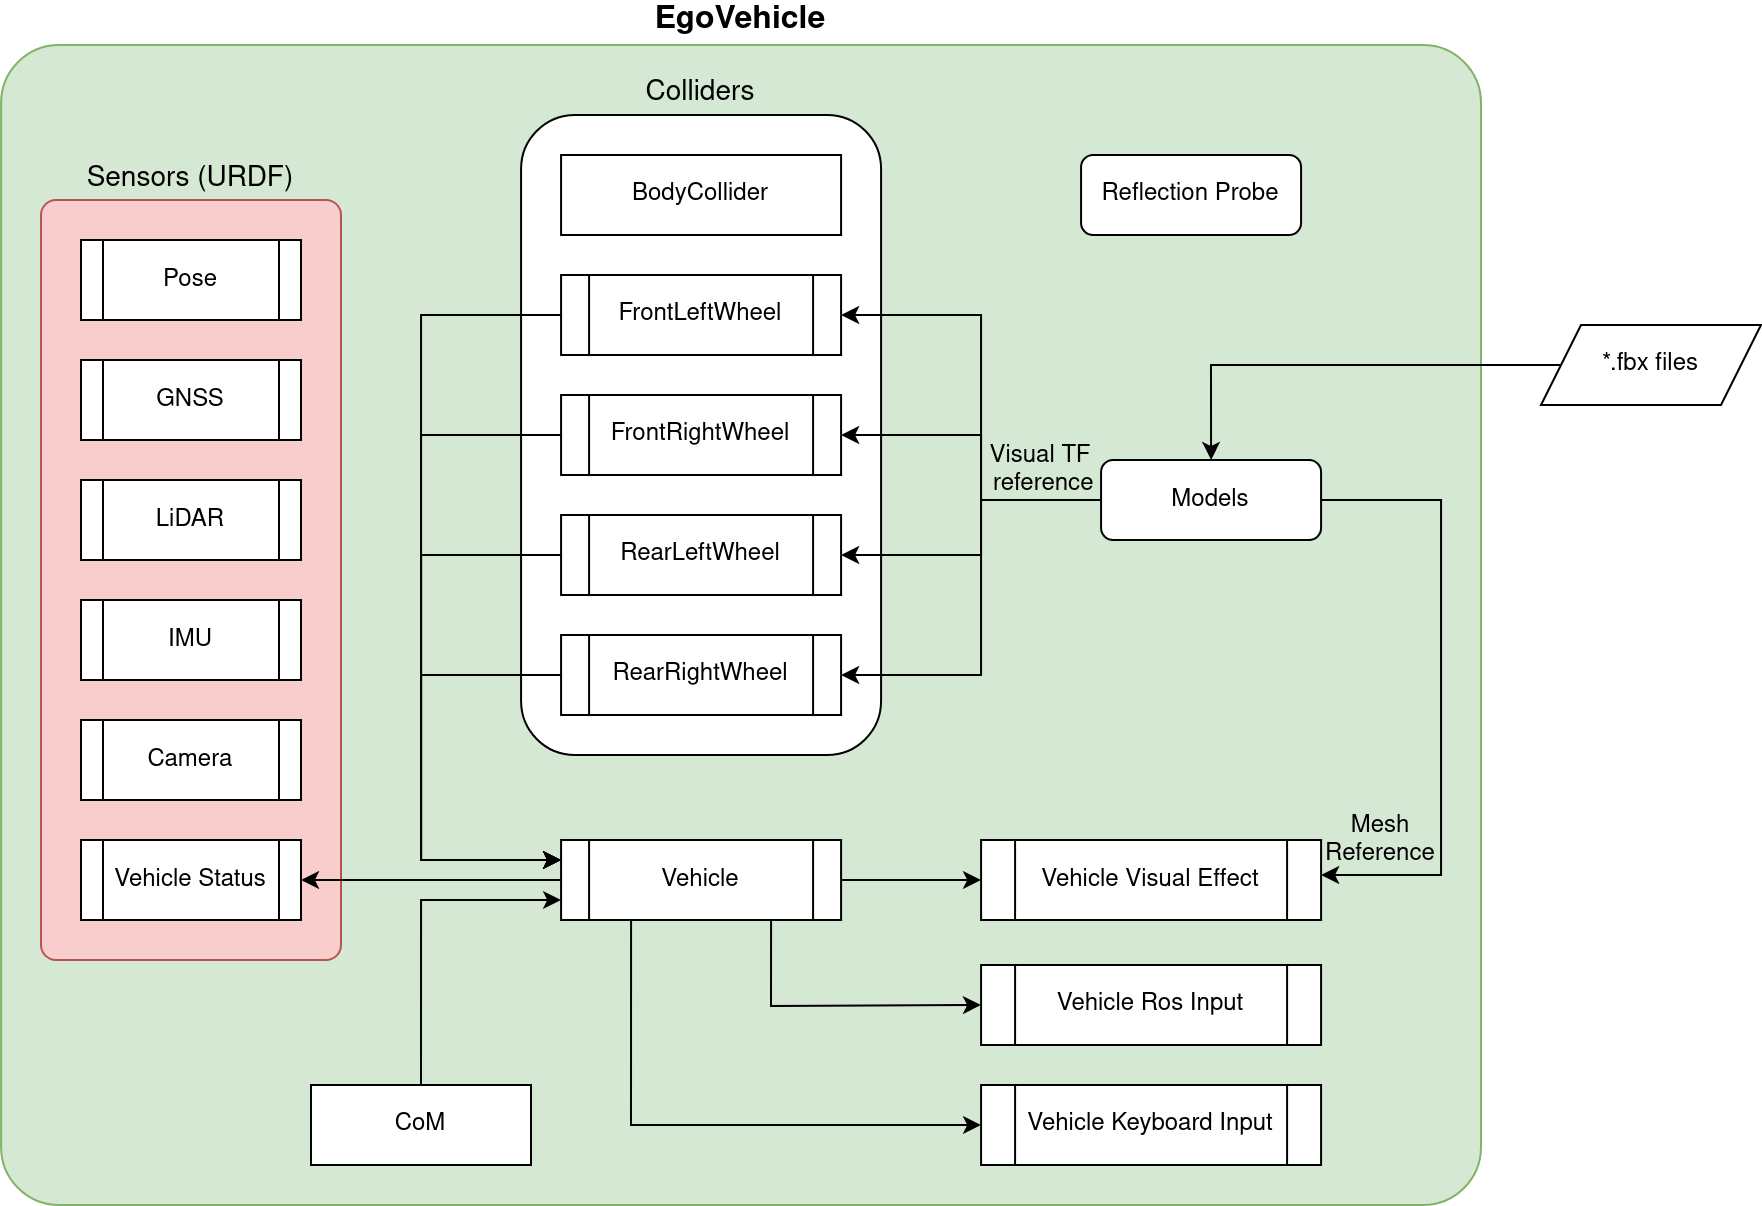
\includegraphics[width=1\linewidth]{figures/AWSIM_EgoVehicle_Architecture.png}
    \caption{معماری مولفه خودروی خودران شبیه‌ساز \lr{AWSIM} \cite{AWSIM:Documentation}}
    \label{fig:AWSIM_EgoVehicle_Architecture}
\end{figure}

مولفه خودروی خودران، یک مؤلفه مسئول برای شبیه‌سازی یک خودروی خودران، حین حرکت در صحنه است. این مولفه شامل موارد زیر می‌شود:
\begin{itemize}
    \item مولفه مدل‌ها \lr{(Models)} و \lr{Reflection Probe} که برای ظاهر دیداری ماشین هستند.
    \item مولفه برخورد‌ دهنده \lr{(Collider)}، که برخورد‌‌ها و قابلیت حرکت ماشین بر روی جاده‌ها را فراهم می‌کند.
    \item مولفه حسگر‌ها که داده‌های مرتبط با وضعیت خودرو در محیط، مانند موقعیت و سرعت آن را فراهم می‌کنند،
    \item مولفه وسیله نقلیه \lr{(Vehicle)}،‌ که دینامیک ماشین را شبیه‌سازی می‌کند و حرکت مولفه‌های چرخ \lr{(Wheel)} را کنترل می‌کند.
    \item مولفه‌های \lr{Vehicle Ros Input} و  \lr{ٰVehicle Keyboard Input} مرجعی به مولفه وسیله نقلیه دارند و دستورهای کنترلی را به آن می‌دهند.
    \item مولفه جلوه‌های بصری وسیله نقلیه ‌\lr{(Vehicle Visual Effects)}، که یک بستر را برای کنترل نورپردازی مولفه وسیله نقلیه، فراهم می‌کند.
\end{itemize}
توضیحات کامل این مولفه، در صفحه توضیحات شبیه‌ساز \lr{AWSIM}، آمده است\LTRfootnote{\url{https://tier4.github.io/AWSIM/Components/Vehicle/EgoVehicle/}}.

\subsection{شبیه‌ساز \lr{AWSIM} و ترکیب آن با \lr{Autoware}}
ترکیب \lr{Autoware} و \lr{AWSIM}، امکان بررسی درستی رفتار خودروی خودران را در سناریو‌های مختلف ترافیکی، فراهم می‌کند. 
\begin{figure}[h!]
    \centering
    \includegraphics[width=0.85\linewidth]{figures/AWSIM_Autoware_Architecture.png}
    \caption{معماری ترکیب \lr{Autoware} و \lr{AWSIM} \cite{AWSIM:Documentation}}
    \label{fig:AWSIM_Autoware_Architecture}
\end{figure}
ترکیب \lr{AWSIM} با \lr{Autoware} به واسطه مولفه‌های بستر خودرو و احساس در معماری \lr{Autoware} امکان‌پذیر است. مولفه مسئول برای اطمینان از ارتباط با این مدول‌ها از سوی \lr{AWSIM}،  مولفه، \lr{EgoVehicle} است. این مولفه، به معماری \lr{Autoware} تطبیق یافته‌ و ارتباط بر اساس مباحث \lr{ROS2} را فراهم می‌کند. با این حال، یک اجزا مهم دیگر به نام انتشار‌کننده زمان وجود دارد که زمان شبیه‌سازی را برای \lr{Autoware} فراهم می‌کند و همچنین بر روی یک مبحث \lr{ROS2} منتشر می‌شود\LTRfootnote{\url{https://tier4.github.io/AWSIM/Components/ROS2/ROS2ForUnity/\#extension-scripts}}.

مؤلفه \lr{EgoVehicle} اطلاعات حال حاضر خودرو را از طریق یک اسکریپت درون مولفه وضعیت خودرو (\lr{Vehicle Status}) منتشر می‌کند. این اطلاعات به صورت بلادرنگ ارائه می‌شود و شامل مواردی نظیر: سرعت جاری، جهت گیری چرخ‌ها یا وضعیت جاری چراغ‌های خودرو است، که از سوی \lr{AWSIM} به‌دست می‌آیند و خروجی‌های آن هستند.

از سوی دیگر، مؤلفه \lr{Vehicle Ros Input}، مسئول ارائه مقادیر خروجی از \lr{Autoware} است. این مؤلفه در دستورات جاری مرتبط با شتاب دادن، دنده‌های گیربکس یا کنترل نورهای مشخص مشترک می‌شود.

اجرای دستورات دریافتی از طریق مؤلفه وسیله نقلیه امکان‌پذیر است، که تنظیم شتاب مناسب بر روی چرخ و کنترل عناصر بصری خودرو را انجام می‌دهد.

سایر داده‌های ارسالی از سوی \lr{AWSIM} به \lr{Autoware}، اطلاعات حسگرها هستند که اطلاعاتی در مورد وضعیت فعلی محیط اطراف و اطلاعات مورد نیاز برای تخمین دقیق موقعیت \lr{EgoVehicle} را فراهم می‌کند\LTRfootnote{\url{https://tier4.github.io/AWSIM/Introduction/CombinationWithAutoware/}} \cite{AWSIM:Documentation}.

\begin{figure}[h!]
    \centering
    \includegraphics[width=0.95\linewidth]{figures/AWSIM_Autoware_Combination.png}
    \caption{تصویری از همکاری شبیه‌ساز \lr{AWSIM} (سمت چپ) و نرم‌افزار \lr{Autoware}} (سمت راست) \cite{AWSIM:Documentation}
    \label{fig:AWSIM_Autoware_Combination}
\end{figure}

\subsection{افزونه \lr{ROS2ForUnity}}
مدول \lr{Ros2ForUnity (R2FU)} یک راه‌حل ارتباطی است که به طور موثر، اتصالی بین موتور بازی‌سازی \lr{Unity} و بستر \lr{ROS2} ایجاد می‌کند و یک ادغام قوی را تشکیل می‌دهد. این مدول، برخلاف راه‌حل‌های دیگر، از ارتباط مستقیم استفاده می‌کند و به‌جای استفاده از پل ارتباطی، از پشته میان‌افزاری \lr{ROS2} (به ویژه کتابخانه کلاینت \lr{rcl} و لایه‌های پایین‌تر آن) استفاده می‌کند، که امکان اضافه کردن گره‌های \lr{ROS2} را به شبیه‌سازی‌های \lr{Unity} را فراهم می‌کند.

\lr{R2FU} در \lr{AWSIM}، به دلایل متعددی استفاده می‌شود. اول از همه‌ چیز، به علت ارائه ادغامی با عملکرد بالا بین \lr{Unity} و \lr{ROS2}، با بهبود توانایی انتقال و کاهش تأخیر نسبت به راه‌حل‌های پل ارتباطی، این مدول قابلیت‌های واقعی \lr{ROS2} را برای موجودیت‌های شبیه‌سازی در \lr{Unity} فراهم می‌کند، پیام‌های استاندارد و سفارشی\LTRfootnote{\lr{Custom}} را پشتیبانی می‌کند و انتزاعات\LTRfootnote{\lr{Abstractions}} و ابزارهای مفیدی را ارائه می‌دهد که همگی به عنوان یک عنصر \lr{Unity} تعبیه شده‌اند.

افرونه \lr{R2FU}، برخی از پیام‌های نرم‌افزارهای \lr{ROS2} و \lr{Autoware} را به صورت پیش‌فرض، پشتیبانی می‌کند که در \cref{tab:R2FU_Messages_Table} مشاهده می‌شوند:
\begin{table}[h!]
    \centering
    \caption{جدول پیام‌های پشتیبانی شده توسط \lr{R2FU} \cite{AWSIM:Documentation}}
    \begin{tabular}{|c|c|}
         \hline
         \textbf{بسته} & \textbf{پیام} \\
         \hline
         \multirow{5}{*}{\textbf{\lr{common\_interfaces}}} & \lr{std\_msgs} \\ & \lr{geometry\_msgs} \\ & \lr{sensor\_msgs} \\ &  \lr{nav\_msgs} \\ & \lr{diagnostic\_msgs} \\
         \hline
         \multirow{4}{*}{\textbf{\lr{rcl\_interfaces}}} & \lr{builtin\_interfaces} \\ & \lr{action\_msgs} \\ & \lr{rosgraph\_msgs} \\ &  \lr{test\_msgs} \\
         \hline
         \multirow{5}{*}{\textbf{\lr{autoware\_auto\_msgs}}} & \lr{autoware\_auto\_control\_msgs} \\ & \lr{autoware\_auto\_geometry\_msgs} \\ & \lr{autoware\_auto\_planning\_msgs} \\ &  \lr{autoware\_auto\_mapping\_msgs} \\ & \lr{autoware\_auto\_vehicle\_msgs} \\
         \hline
         \multirow{2}{*}{\textbf{\lr{tier4\_autoware\_msgs}}} & \lr{tier4\_control\_msgs} \\ & \lr{tier4\_vehicle\_msgs} \\
         \hline
         \multirow{2}{*}{\textbf{\lr{others}}} & \lr{tf2\_msgs} \\ & \lr{unique\_identifier\_msgs} \\
         \hline
    \end{tabular}
    \label{tab:R2FU_Messages_Table}
\end{table}
برای اینکه بسته پیامی سفارشی را بتوان در \lr{Unity} استفاده کرد، بایستی فایل‌های \lr{*.dll} و \lr{*.so} آن توسط \lr{R2FU} ساخته شوند\LTRfootnote{\url{https://tier4.github.io/AWSIM/Components/ROS2/ROS2ForUnity/}} \cite{AWSIM:Documentation}.

\section{موتور بازی \lr{Unity}}
\lr{Unity}، یک موتور بازی\LTRfootnote{\lr{Game Engine}} و سکو توسعه‌ی گسترده است که در صنایع بازی و رسانه‌های تعاملی بسیار محبوب است. این موتور بازی، به دلیل چند منظوره گرایی و دسترسی آسان شناخته شده است و به موتور انتخابی برای توسعه‌دهندگان تبدیل شده است، که قصد دارند محتوای گسترده‌ای از بازی‌های کامپیوتری تا برنامه‌های واقعیت افزوده و شبیه‌سازی‌ها را ایجاد کنند. \lr{Unity} سکو‌های مختلف را پشتیبانی می‌کند و این امکان را به توسعه‌دهندگان می‌دهد که پروژه‌های خود را بر روی دستگاه‌های مختلف مانند کامپیوتر شخصی، تلفن همراه، کنسول و حتی هدست‌های واقعیت مجازی/افزوده اجرا کنند. فروشگاه عناصر یونیتی دارای مجموعه‌ای بزرگ از منابع پیش‌ساخته، اسکریپت‌ها و ابزارها است که توسعه‌ی پروژه‌ها را ساده‌تر و سریع‌تر می‌کند، در حالی که سیستم اسکریپت‌نویسی بصری‌اش به نام "\lr{Bolt}" به افرادی که برنامه‌نویس نیستند اجازه می‌دهد تا رفتارها و تعامل‌های پیچیده‌ای را ایجاد کنند. اسکریپت‌های این موتور، با زبان برنامه‌نویسی \lr{C\#} نوشته می‌شوند.

\begin{figure}[h!]
    \centering
    \includegraphics[width=1\linewidth]{figures/Unity_Workspace.png}
    \caption{شبیه‌ساز \lr{AWSIM} در بستر موتو بازی \lr{Unity} \cite{AWSIM:Documentation}}
    \label{fig:Unity_Workspace}
\end{figure}

یکی از ویژگی‌های برجسته‌ی \lr{Unity}، توانایی پردازش بلادرنگ آن است، که تجربیاتی با کیفیت بالای بصری و تعاملی را ارائه می‌دهد. این موتور امکان نورپردازی و سایه‌دهی پویا، شبیه‌سازی فیزیکی و پشتیبانی از گرافیک‌های دو‌بعدی و سه‌بعدی را فراهم می‌کند که همگی اساسی برای ایجاد جهان‌های غنی و شبیه‌سازی‌های واقع‌گرایانه هستند. به علاوه، رابط کاربری کاربر پسند این موتور، به جفت توسعه‌دهندگان مبتدی و حرفه‌ای این امکان را می‌دهد که پروتوتایپ‌سازی و تکرار سریع ایده‌های خود را به واقعیت تبدیل کنند. با جامعه‌ی پررونق توسعه‌دهندگان و مستندات جامع، یونیتی همچنان در حال تکامل است و خالقان را به اجرای ایده‌های خلاقانه خود ترغیب می‌کند و موقعیت برتری را به عنوان یکی از موتورهای اصلی صنعت بازی،‌برای خود تثبیت می‌کند\LTRfootnote{\url{https://unity.com/}}.

\section{ابزار \lr{Blender}}
\lr{Blender} یک ابزار قدرتمند و چندکاره در دنیای مدل‌سازی سه‌بعدی، انیمیشن و رندرینگ\LTRfootnote{\lr{Rendering}} است که به عنوان یک نرم‌افزار متن‌باز معرفی شده و در دنیای مدل‌سازی سه‌بعدی، انیمیشن و رندرینگ جایگاه ویژه‌ای دارد. این نرم‌افزار به خاطر داشتن مجموعه‌ای گسترده از امکانات معروف است، که از مدل‌سازی سه‌بعدی و نقاشی تا ریگینگ\LTRfootnote{\lr{Rigging}}، انیمیشن و حتی ویرایش ویدیویی می‌پردازد. رابط کاربری دوستانه \lr{Blender}، به همراه مجموعه گسترده ابزار و امکانات، آن را مناسب برای جفت مبتدیان و هنرمندان ماهر می‌کند. این نرم‌افزار به دلیل عملکرد قوی خود و همچنین به عنوان یک جایگزین مقرون به صرفه برای راه‌حل‌های نرم‌افزاری سه‌بعدی متعلق به شرکت‌های مختلف، شناخته شده است. این ابزار، برای کار روی انیمیشن‌های پیچیده شخصیتی، تصویرسازی‌های معماری یا اشیاء بازی، ‌\lr{Blender} مجموعه‌ای جامع از ابزارها را فراهم می‌کند.

\begin{figure}[h!]
    \centering
    \includegraphics[width=1\linewidth]{figures/Blender.png}
    \caption{محیط ابزار \lr{Blender}}
    \label{fig:Blender}
\end{figure}

یکی از ویژگی‌های برجسته \lr{Blender}، ادغام آسان آن با \lr{Unity} است. یونیتی به طور پیش‌فرض، امکان وارد کردن فایل‌های \lr{Blender} را پشتیبانی می‌کند، که امکان بارگذاری مدل‌ها و انیمیشن‌های ایجاد شده در \lr{Blender} به طور مستقیم در پروژه‌های یونیتی را فراهم می‌کند. این سازگاری جریان کار را تسهیل می‌کند، زمان طی شده در فرآیند کار را کاهش می‌دهد و به هنرمندان اطمینان می‌دهد که بتوانند محتوای خود را در \lr{Blender} ایجاد کرده و آن را به سرعت در محیط \lr{Unity} مشاهده کنند. ترکیب قدرتمند مدل‌سازی سه‌بعدی و انیمیشن این ابزار، با ابزارهای توسعه بازی همانند \lr{Unity}، دنیایی از امکانات خلاقانه را ارائه می‌دهد و به توسعه‌دهندگان این امکان را می‌دهد تا محیط‌ها، شخصیت‌ها و اشیاء بازی را به راحتی طراحی و نمونه‌سازی کنند\LTRfootnote{\url{https://www.blender.org/}}.

\subsection{افزونه \lr{Blosm}}
\lr{Blosm}، که قبلاً به عنوان \lr{Blender-OSM} شناخته می‌شد، یک افزونه قدرتمند برای \lr{Blender} است که طراحی شده تا فرآیند وارد کردن داده‌ها و نقشه‌های جغرافیایی را ساده‌تر کند. با تنها چند کلیک، این افزونه دسترسی به مجموعه‌ای گسترده از منابع داده‌ای فراهم می‌کند، از جمله شهرهای سه‌بعدی گوگل، اطلاعات \lr{OpenStreetMap} و داده‌های پستی بلندی جهانی. این ابزار چند منظوره به کاربران این امکان را می‌دهد که به آسانی جزئیات جغرافیایی واقعی را به پروژه‌های \lr{Blender} خود وارد کنند. \lr{Blosm}، یک پروژه متن‌باز است. قابلیت‌های این افزونه بسیار قدرتمند است و به کاربران این امکان را می‌دهد تا انواع عناصر از جمله ساختمان‌ها، اشیاء آبی مانند رودخانه‌ها و دریاچه‌ها، مناطق گیاهی، جاده‌ها، مسیرها، راه‌آهن‌ها و داده‌های دقیق زمین با وضوح پوشش جهانی تقریباً 30 متر را وارد کنند\LTRfootnote{\url{https://github.com/vvoovv/blosm/wiki/Documentation}}.

\section{ابزار \lr{OpenStreetMap}}

ابزار طراحی نقشه‌برداری \lr{OpenStreetMap (OSM)}، یک پروژه مشترک و متن‌باز است که یک مخزن گسترده از داده‌های مکانی ارائه می‌دهد، شامل نقشه‌های دقیق و اطلاعات جغرافیایی که توسط داوطلبان از سراسر جهان تهیه می‌شود. این مشارکت‌ها مجموعه‌ای وسیع از ویژگی‌های جغرافیایی از جمله جاده‌ها، نمادها، شهرها و موارد دیگر را در بر می‌گیرد، که از مهم‌ترین منابع برای برنامه‌هایی مانند ناوبری، برنامه‌ریزی شهری، مدیریت بحران و خدمات مکانی مختلف هستند. مدل داده باز \lr{OSM}، کاربران را تشویق به ویرایش و بهبود نقشه‌ها می‌کند، تضمین می‌کند که داده‌های این پلتفرم به‌روز می‌شود و برای مجموعه‌ای گسترده از موارد کاربردی معتبر باقی می‌ماند.

\begin{figure}[h!]
    \centering
    \includegraphics[width=1\linewidth]{figures/Amirkabir_OpenStreetMap.png}
    \caption{نقشه دانشگاه صنعتی امیرکبیر در ابزار \lr{OSM}}
    \label{fig:Amirkabir_OpenStreetMap}
\end{figure}

\section{کتابخانه \lr{OusterSDK}}
کتابخانه توسعه نرم‌افزار حسگرهای لایدار شرکت \lr{Ouster}، واسطه‌هایی را برای تعامل با سخت‌افزار حسگر و داده‌های حسگر ضبط‌شده که برای انجام آزمون‌ها، ارزیابی، و برنامه‌های غیرمرتبط با ایمنی، مناسب هستند را در زبان‌های پایتون و \lr{C++} فراهم می‌کند. کدهای مثال و مرجع برای عملیات معمول بر روی داده‌های حسگر در هر دو زبان نیز ارائه شده است. این کتابخانه، شامل واسط‌های برنامه‌نویسی برای:
\begin{enumerate}
    \item پرس‌‌وجوی تنظیمات حسگر و تنظیمات آنها
    \item ضبط و خواندن داده‌ها به فرمت \lr{.pcap}
    \item خواندن و بافرینگ داده‌های \lr{UDP} به صورت قابل اطمینان
    \item تبدیل داده‌های خام به تصاویر فاصله\LTRfootnote{\lr{Range}}، سیگنال، \LTRfootnote{\lr{Signal}}نور مادون قرمز نزدیک\LTRfootnote{\lr{Near-IR}}، انعکاس‌پذیری\LTRfootnote{\lr{Reflectivity}}
    \item  تبدیل اندازه‌گیری‌های کانال فاصله به مختصات کارتزین $(x, y, z)$
\end{enumerate}
علاوه بر این، این کتابخانه در زبان پایتون قابلیت‌های زیر را نیز دارد:
\begin{enumerate}
    \item دسترسی به فریم‌های داده‌های لایدار به عنوان داده‌های \lr{numpy}
    \item یک ابزار نمایشگر برای داده‌های ضبط شده‌ی \lr{.pcap} و حسگر لایدار \cite{OusterSDK:Documentation} (\cref{fig:OusterSDK_Visualizer})
\end{enumerate}

\begin{figure}[h!]
    \centering
    \includegraphics[width=1\linewidth]{figures/OusterSDK_Visualizer.png}
    \caption{ابزار نمایشگر کتابخانه \lr{OusterSDK} برای ابر نقاط \cite{OusterSDK:Documentation}}
    \label{fig:OusterSDK_Visualizer}
\end{figure}

\section{ابزار \lr{Ouster Studio}}
ابزار \lr{Ouster Studio} یک نرم‌افزار قدرتمند و کاربرپسند است که برای پردازش و نمایش داده‌های لایدار توسعه یافته است. با \lr{Ouster Studio}، شما می‌توانید به سرعت و سادگی داده‌های لایدار \lr{Ouster} را وارد کرده، تجزیه و تحلیل کرده و نمایش دهید. این نرم‌افزار برای ساده‌تر کردن فرآیند تنظیم و نمایش حسگرها ساخته شده و با کشف خودکار حسگر، امکان تشخیص و شناسایی حسگرهای متصل به یک شبکه یا سیستم را فراهم می‌کند. علاوه بر این، امکان پخش زنده، به کاربران این امکان را می‌دهد که داده‌های حسگر را به صورت بلادرنگ دریافت و پردازش کنند، که می‌تواند برای به دست آوردن بینش‌های فوری و امکان تصمیم‌گیری به موقع، مفید باشد. این نرم‌افزار به شما این امکان را می‌دهد که داده‌ها را به سرعت خود مرور و مطالعه کنید؛ همچنین امکان به اشتراک گذاری ضبط‌ داده‌های لایدار ضبط شده و شناسایی الگوها و روندهای آن را فراهم می‌کند، که ممکن است در داده‌های بلادرنگ به سرعت مشخص نشود.
\chapter{پیاده‌سازی و طراحی}
در این فصل، به چگونگی پیاده‌سازی پروژه و طریقه شکل‌گیری دوقلوی دیجیتال خیابان رشت می‌پردازیم.

\section{نگاهی به مسیر طی شده}
از آنجایی که این پروژه، پژوهشی بزرگ محسوب می‌شود، نیاز است تا فلوچارتی\LTRfootnote{\lr{Flowchart}} برای درک آن کشیده شود.

\begin{figure}[h!]
    \centering
    \includegraphics[width=1\linewidth]{figures/Project_Flowchart.png}
    \caption{فلوچارت پروژه}
    \label{fig:Project_Flowchart}
\end{figure}

همانطور که طبق \cref{fig:Project_Flowchart} مشاهده می‌شود، اولین سوالی که پیش‌ می‌آید، امکان‌پذیر بودن این پژوهش است.

\section{سناریو اول: استفاده از داده‌های نمونه}
گرفتن مجوز برای داده‌برداری از خیابان رشت و هماهنگی‌های لازم آن، هزینه‌بر است و تا زمانی که نتوان از امکان‌پذیر بودن این پژوهش اطمینان حاصل یافت، نمی‌توان آن را انجام داد. به همین دلیل، در ابتدا سناریو اول پیش گرفته شد که در آن، اقدام به شبیه‌سازی داده‌های نمونه موجود در تارنمای\LTRfootnote{\lr{Website}} شرکت \lr{Ouster} شده است.

\subsection{پیدا کردن داده‌های نمونه لایدارهای شرکت \lr{Ouster}}
تارنمای شرکت \lr{Ouster}، داده‌های نمونه‌ای را در اختیار توسعه‌دهندگان گذاشته است. یکی از این داده‌های نمونه، حسگر لایداری است که بر روی یک چراغ راهنمایی رانندگی، در یک چهارراه نصب شده است \LTRfootnote{\url{https://data.ouster.dev/\#/share/7LQRDQD3APIJL15L}}. 

\begin{figure}[h!]
    \centering
    \includegraphics[width=1\linewidth]{figures/Ouster_Sample_Data_Intersection.png}
    \caption{داده‌ی نمونه که با لایدار \lr{OS1:128} ضبط شده است.}
    \label{fig:Ouster_Sample_Data_Intersection}
\end{figure}

با توجه به \cref{fig:Ouster_Sample_Data_Intersection}، مشاهده می‌شود که می‌توان داده‌‌ نمونه را بر روی کامپیوتر شخصی نیز دریافت کرد. داده‌های ابرنقاط عموما حجیم هستند و به طور مثال، داده فوق حدود ۲ گیگابایت\LTRfootnote{\lr{Gigabyte}} حجم دارد. 

\section{انتخاب مدل هوش مصنوعی تشخیص سه‌بعدی و ردیاب}
حال زمان آن رسیده است که مدل هوش مصنوعی‌ تشخیص دهنده‌ای را برای این پژوهش انتخاب کرد. در این پژوهش، تشخیص اجسام تنها با استفاده از ابر نقاط صورت می‌گیرد. از فصل مفاهیم پایه به یاد داریم که سه روش مختلف برای تشخیص اجسام سه‌بعدی استفاده می‌شود. عموما سرعت مدل‌های مبتنی بر واکسل، از دیگر روش‌ها بیشتر است و از آنجایی که در این پژوهش، داده‌های ورودی بلادرنگ هستند، بایستی سرعت مدل جدی گرفته شود. با جستجو و تحقیقات در مورد مدل‌های تشخیص اجسام سه بعدی، به چند مخزن\LTRfootnote{\lr{Repository}} و مقاله دست‌ یافته شده است.

\subsection{مدل \lr{SFA3D}}
این مخزن معروف، مدلی بسیار سریع است که از مجموعه داده \lr{KITTI} برای تمرین و آزمون استفاده می‌کند. 
\begin{figure}[h!]
    \centering
    \includegraphics[width=0.75\linewidth]{SFA3D.png}
    \caption{تشخیص بلادرنگ مدل \lr{SFA3D}، با سرعت تشخیص بیشتر از ۹۰ فریم در ثانیه \cite{Super-Fast-Accurate-3D-Object-Detection-PyTorch}}
    \label{fig:SFA3D}
\end{figure}
در ابتدا این مدل ایده‌آل به نظر می‌رسید، اما مشکلاتی دارد که عبارتند از:
\begin{enumerate}
    \item این مدل از مجموعه داده \lr{KITTI} استفاده می‌کند که نسبت به دو مجموعه داده \lr{Waymo Open} و \lr{nuScenes}، بسیار ناقص‌تر است. این مدل بر روی مجموعه داده \lr{KITTI} خوب عمل می‌کند، اما در عمل با افت دقت روبرو خواهد شد.
    \item این مدل، سیستمی برای ردیابی و انتساب شناسه به اجسام ندارد.
    \item این مدل نسبتا قدیمی است و مدل‌های بهتر و قوی‌تری وجود دارند.
\end{enumerate}

\subsection{مخزن \lr{MMDetection3D}}
مخزن \lr{MMDetection3D}، یک جعبه‌ابزار متن‌باز برای تشخیص اجسام سه‌بعدی است. این مخزن توسط شرکت \lr{OpenMMLab}\LTRfootnote{\url{https://openmmlab.com/}} از کشور چین ساخته شده است، که جعبه‌ابزارهایی را در انواع زمینه‌های هوش مصنوعی، طراحی کرده است. کاربران با توجه به نیازمندی خود، می‌توانند به مخزن هر کدام از این جعبه‌ابزارها مراجعه کنند. این جعبه‌ابزارها بسترهایی هستند که با استفاده از آنها، کاربران می‌توانند مدل‌های دلخواه خود را انتخاب کنند و تنها با دریافت کردن مجموعه‌داده مورد نیاز، مدل انتخاب شده را آموزش دهند. به طور مثال، در مخزن \lr{MMDetection3D}، بیش از ۳۰۰ مدل مختلف پیاده‌سازی شده‌اند و مدل‌های جدید همواره در حال پیاده‌سازی و اضافه شدن به این مخزن هستند.

\begin{figure}
    \centering
    \includegraphics[width=0.75\linewidth]{figures/MMDetection3D_Models.png}
    \caption{تعداد مدل‌های پیاده‌سازی شده در مخزن \lr{MMDetection3D} \cite{mmdet3d2020}}
    \label{fig:MMDetection3D}
\end{figure}

طبق \cref{fig:MMDetection3D}، می‌توان مشاهده کرد که این مخزن در حال حاضر ۱۰۷ عدد مدل ابرنقاط محور مبتنی بر واکسل دارد و از معماری \lr{PointPillars} استفاده می‌کنند. یکی از مدل‌های معروف این مخزن، که در سال ۲۰۲۱ ساخته شد و همچنان از آن استفاده می‌شود، مدل \lr{CenterPoint}\cite{yin2021center} است.

\subsubsection{مدل تشخیص اجسام سه‌بعدی \lr{CenterPoint}}
اشیاء سه‌بعدی معمولاً به عنوان کادرهای محصور‌کننده سه‌بعدی در ابرنقاط نمایش داده می‌شوند. این نمایش، شبیه کشف کادر‌های محصورکننده دوبعدی بر پایه تصویر است، اما در فضای سه‌بعدی با مشکلاتی مواجه می‌شود. اشیاء در جهان سه‌بعدی هیچ جهت خاصی را دنبال نمی‌کنند و  مدل‌های مبتنی بر این کادرها، مشکلاتی در شمارش تمام جهت‌ها یا تلفیق یک کادر مرزی تطابقی به اشیاء چرخان دارند. اما در این مقاله، اشیاء سه‌بعدی به عنوان یک سری نقاط، نمایش، تشخیص و ردیابی می‌شوند. چهارچوب این مدل، \lr{CenterPoint}، ابتدا مراکز اشیاء را با استفاده از یک تشخیص‌دهنده نقاط کلیدی\LTRfootnote{\lr{Keypoint Detector}} یافته و سپس به ویژگی‌های دیگر از جمله اندازه سه‌بعدی، جهت سه‌بعدی و سرعت بازمی‌گرداند. در مرحله دوم، این تخمین‌ها را با استفاده از ویژگی‌های نقطه‌ای دیگر استنتاج شده از اجسام، بهبود می‌دهد. در مدل \lr{CenterPoint}، ردیابی اجسام سه‌بعدی با تطبیق حریصانه به نزدیک‌ترین نقطه\LTRfootnote{\lr{Greedy Closest-Point Matching}} ساده‌سازی می‌شود زیرا اجسام به نقاط معارف آن جسم تصویر شده‌اند. الگوریتم تشخیص و ردیابی حاصل، ساده، کارآمد و موثر است. \lr{CenterPoint} عملکرد برجسته‌ای را در آزمایش‌های آنلاین مجموعه داده \lr{nuScenes} در رده‌بندی‌های تشخیص و ردیابی سه‌بعدی، به ثبت رساند. این مدل با ۵.۶۵ امتیاز \lr{NDS} و ۸.۶۳ امتیاز \lr{AMOTA} برای یک مدل مبتنی بر ابر نقاط، به بهترین عملکرد ممکن در زمان خود رسید. این مدل در مجموعه داده  \lr{Waymo Open}، تمام روش‌های مدل تک‌مرحله‌ای قبلی را با اختلاف زیادی پیش‌می‌گیرد و در میان تمام مدل‌های مبتنی بر ابر نقاط، جایگاه اول را در سال ۲۰۲۱ گرفت \cite{yin2021center}.

\begin{figure}[h!]
    \centering
    \includegraphics[width=1\linewidth]{figures/Centerpoint_Architecture.png}
    \caption{معماری مدل \lr{CenterPoint} \cite{yin2021center}}
    \label{fig:CenterPoint_Architecture}
\end{figure}

\begin{table}[h!]
    \centering
    \caption{جدول مقایسه مدل‌های سه‌بعدی براساس ارزیابی مجموعه داده \lr{Waymo Open} \cite{yin2021center}}
    \begin{tabular}{cccccc}
        \hline
        \multirow{2}{*}{\textbf{سختی}} & \multirow{2}{*}{\textbf{مدل}} & \multicolumn{2}{c}{\textbf{خودرو}} &\multicolumn{2}{c}{\textbf{عابر پیاده}}\\
        & & \lr{mAP} & \lr{mAPH} & \lr{mAP} & \lr{mAPH}\\
        \hline
        & \lr{StarNet} & 5.61 & 0.61 & 8.67 & 9.59 \\
        & \lr{PointPillars} & 3.63 & 8.62 & 1.62 & 2.50 \\
        \lr{Level 1} & \lr{PPBA} & 5.67 & 0.67 & 7.69 & 7.61 \\
        & \lr{RCD} & 0.72 & 6.71 & - & -\\
        & \lr{CenterPoint} & \textbf{2.80} & \textbf{7.79} & \textbf{3.78} & \textbf{1.72}\\
        \hline
        & \lr{StarNet} & 9.54 & 5.54 & 1.61 & 0.54 \\
        & \lr{PointPillars} & 6.55 & 1.55 & 9.55 & 1.45 \\
        \lr{Level 2} & \lr{PPBA} & 6.59 & 1.59 & 0.63 & 8.55 \\
        & \lr{RCD} & 1.65 & 7.64 & - & -\\
        & \lr{CenterPoint} & \textbf{2.72} & \textbf{8.71} & \textbf{2.72} & \textbf{4.64}\\
        \hline
    \end{tabular}
    \label{tab:R2FU_Messages_Table}
\end{table}

\begin{table}[h!]
    \centering
    \caption{جدول مقایسه مدل‌های سه‌بعدی براساس ارزیابی مجموعه داده \lr{nuScenes} \cite{yin2021center}}
    \begin{tabular}{cccc}
        \hline
        \textbf{روش} & \lr{mAP$\uparrow$} & \lr{NDS$\uparrow$} & \lr{PKL$\downarrow$}\\
        \hline
        \lr{WYSIWYG} & 0.35 & 9.41 & 14.1\\
        \lr{PointPillars} & 1.40 & 0.55 & 00.1\\
        \lr{CVCNet} & 3.55 & 4.64 & 92.0\\
        \lr{PointPainting} & 4.46 & 1.58 & 89.0\\
        \lr{PMPNet} & 4.54 & 1.53 & 81.0\\
        \lr{SSN} & 3.46 & 9.56 & 77.0\\
        \lr{CBGS} & 9.52 & 3.63 & 77.0\\
        \hline
        \lr{CenterPoint} & \textbf{0.58} & \textbf{5.65} & \textbf{69.0}\\
        \hline
    \end{tabular}
    \label{tab:R2FU_Messages_Table}
\end{table}

  این مدل، در مخزن \lr{MMDetection3D} نیز پیاده‌سازی شده است و برای این پژوهش، ایده‌آل است. در ابتدا سعی در نصب این مخزن شد و اقدام به آموزش این مدل شد. اما موقع آموزش مدل \lr{Centerpoint}، با چالش‌هایی روبرو شدیم:
  \begin{itemize}
      \item مجموعه داده \lr{nuScenes}، دارای حجمی حدود ۱ ترابایت\LTRfootnote{\lr{Terabyte}} است و محدودیت حجمی کامپیوتر، مانع فرایند آموزش می‌شود. مجموعه داده آموزشی \lr{Waymo Open} نیز بسیار حجیم است.
      \item به علت داشتن مجموعه داده‌ای عظیم برای آموزش، آموزش این مدل مدت زمان بسیار زیادی را نیاز خواهد داشت.
  \end{itemize}

  با وجود این دشواری‌ها، به نظر می‌آمد که نمی‌توان مدل تشخیص دهنده سه‌بعدی‌ای را آموزش داد. پس تنها راه باقی مانده، استفاده از مدل‌های از پیش آموزش دیده است.

  \subsection{ایده:‌ نگاه انداختن به معماری \lr{Autoware}}
  در بخش قبل نتیجه گرفته شده که به یک مدل تشخیص اجسام سه‌بعدی آماده و از پیش آموزش دیده نیاز است. پس بایستی به دنبال چنین مدلی گشت. حال سوالی پیش می‌آید: مگر خودرو‌های خودران نیاز به تشخیص بلادرنگ اجسام در محدودیت‌های زمانی چند دهم ثانیه‌ای نیستند؟ این خودرو‌ها نیز قطعا در داخل معماری خود، از یک مدل تشخیص اجسام استفاده می‌کنند. همچنین از آنجایی که مسیر حرکت وسایل نقلیه اطراف و سرعت آنها نیز برای این خودروها مهم است، پس قطعا مجهز به یک ردیاب نیز هستند. پس گام بعدی پژوهش، نگاه انداختن به معماری محبوب‌ترین ابزار توسعه خودروهای خودران یا همان \lr{Autoware} بود. در فصل قبل، معماری مولفه‌های مهم برای پژوهش این ابزار، به صورت دقیق بررسی شدند. این معماری‌ها، در اصل برای پیدا کردن مدل هوش مصنوعی و ردیاب مورد استفاده آن‌ها مطالعه شده‌اند. 

\subsection{مولفه ادارک نرم‌افزار \lr{Autoware}}
  
  طبق \cref{fig:Autoware_Perception_Detection_Node_Graph}، در معماری مولفه ادراک \lr{Autoware}، گره‌ای به نام گره \lr{lidar\_centerpoint} وجود دارد. این گره، همان مدل هوش‌ مصنوعی انتخابی برای آموزش در این پژوهش است. توسعه‌دهندگان ابزار \lr{Autoware}، با استفاده از همان مخزن \lr{MMDetection3D} و با استفاده از مجموعه داده آموزشی \lr{nuScenes}، مدل \lr{CenterPoint} را آموزش داده‌اند. آنها در معماری مدل خود، از مدل هسته‌ \lr{PointPillars}، که توسط محققین \lr{NVIDIA} ساخته شده است، استفاده کرده‌اند. این مدل هسته، سرعت چشم‌گیری دارد زیرا از شبکه‌های عصبی \lr{TensorRT} استفاده می‌کند \cite{lang2019pointpillars}.
  
  همچنین با نگاهی دقیق‌تر به معماری مولفه ادارک، متوجه گره \lr{multi\_object\_tracker}، یا ردیاب هم‌زمان چند جسم، می‌شویم.
  تمامی ردیاب‌ها از الگوریتمی به نام ارتباط داده\LTRfootnote{\lr{Data Association}} استفاده می‌کنند. ارتباط داده‌ها، به فرآیند ارتباط دادن یا متناظر کردن مشاهدات (نقاط داده\LTRfootnote{\lr{Data Points}}) از حسگرها، مانند داده‌هایی که از حسگر‌های ادراکی مثل لایدار یا رادار جمع‌آوری شده‌اند، به اشیائی خاص یا ردهایی در محیط اشاره دارد. هدف این است که تعیین شود کدام مشاهدات هوش مصنوعی، به کدام اشیاء در فریم قبلی به صورت دقیق متناظر می‌شوند.

الگوریتم‌های ارتباط داده، مسئله‌ای به نام تطبیق امتیاز بیشینه\LTRfootnote{\lr{Maximum Score Matching}} دارند، که اشاره به یک روش دارد که به دنبال یافتن بهترین ارتباطات بین مشاهدات و اشیاء یا ردها، براساس یک امتیاز یا هزینه می‌باشد. این فرآیند گاهی به عنوان "مسئله حداقل هزینه حداکثر جریان\LTRfootnote{\lr{Minimum Cost Maximum Flow}}" نیز شناخته می‌شود و معمولاً با استفاده از الگوریتم‌هایی مانند حل‌کننده \lr{muSSP} حل می‌شود. این حل‌کننده، اتصال بهینه مشاهدات به اشیاء را با کمینه کردن هزینه کل ارتباطات بهینه می‌کند، که ممکن است شامل فاکتورهایی مانند مساحت شیء از نمای دید پرنده، فاصله ماهالانوبیس و حداکثر فاصله باشد. این معیارها به تعیین کیفیت ارتباط بین یک مشاهده و یک شیء کمک می‌کنند.

\begin{figure}[h!]
    \centering
    \includegraphics[width=0.5\linewidth]{figures/Autoware_Multi_Object_Tracking_Architecture.png}
    \caption{نحوه کارکرد گره ردیاب هم‌زمان چند جسم}
    \label{fig:Autoware_Multi_Object_Tracker}
\end{figure}

در گره ردیاب هم‌زمان چند جسم، از فیلتر‌های کالمن تعمیم‌یافته شده\LTRfootnote{\lr{EKF-Filter}} استفاده 
می‌شود تا وضعیت انواع اجسام مختلف حاضر در صحنه را تخمین بزند. این گره، مدل‌های ویژه‌ای را برای عابرین پیاده، دوچرخه‌‌ها، خوردو‌ها و وسایل نقلیه بزرگ تعریف کرده است، زیرا ابعاد آن‌ها بسیار متفاوت است و یک فیلتر کالمن جوابگوی تمام حالات نیست. این مدل‌ها به صورت موازی اجرا می‌شوند و بدین شکل، یک سیستم ردیاب پایدار و دقیق پیاده‌سازی می‌شود \cite{AWSIM:Documentation}.

\subsection{نتیجه‌گیری}
در این بخش، به این نتیجه رسیده شد که آموزش مدل‌های تشخیص اجسام سه‌بعدی، نیاز به مجموعه داده‌های عظیم دارد که خارج از توانایی این پژوهش است. راه‌حل پیشنهادی، استفاده از مدل‌های از پیش آموزش داده شده است. ایده‌ای که در این زمینه زده شد، استفاده از مدل هوش مصنوعی مورد استفاده ابزار \lr{Autoware}، برای تشخیص و ردیابی اجسام است. 

\section{اعمال مدل هوش‌ مصنوعی به ورودی لایدار}
در بخش قبلی، به این نتیجه رسیدیم که می‌توان از مدل‌ \lr{CenterPoint} مورد استفاده در ابزار \lr{Autoware}، به عنوان تشخیص دهنده اجسام استفاده کرد. همچنین می‌توان از گره ردیاب هم‌زمان چند جسم آن، برای ردیابی اجسام تشخیص داده شده استفاده کرد. با نگاهی دیگر به \cref{fig:Autoware_Perception_Detection_Node_Graph} که گراف گره مولفه ادراک است، درمی‌یابیم که گره‌ی \lr{lidar\_centerpoint}، دارای اشتراکی به یک مبحث\LTRfootnote{\lr{/sensing/lidar/concatenated/pointcloud}} است. این مبحث، خروجی پیش‌پردازش صورت گرفته بر روی ابر نقاط خام لایدار‌های خودروی خودران است. پس گمان می‌رود که با انتشار ابر نقاط خود به این مبحث، بتوانیم از لایه‌ی ادراک استفاده کنیم، که یعنی عملیات تشخیص و ردیابی بر روی ابر نقاط داده‌ی نمونه ما انجام شود.

جنس داده‌‌ی این مبحث، از نوع پیام‌های \lr{sensor\_msgs/PointCloud2} است. اما فرمت داده‌های ضبط شده‌ی لایدارهای شرکت \lr{Ouster}، فرمت \lr{*.pcap} است که در داخل آن بسته‌های\LTRfootnote{\lr{Packet}} شبکه‌ای لایدار ذخیره شده‌اند. پس نیاز است که این بسته‌ها در درجه اول پردازش شوند، و سپس اطلاعات ابر نقاط داخل هر بسته آن به پیامی از جنس \lr{PointCloud2}، که از پیام‌های پیش‌فرض برای ابر نقاط در بستر \lr{ROS2} است، تبدیل بشوند. به همین منظور، کدی در بستر \lr{ROS2} نوشته شد، که داده‌های بلادرنگ یا ضبط‌ شده‌ی لایدار‌های \lr{Ouster} را به ابر نقاط مورد استفاده در \lr{ROS2}، تبدیل کند. 
این بسته \lr{ROS2} که \lr{"pcap\_to\_pointcloud2\_publisher\_py"} نام دارد، با استفاده از کتابخانه کلاینت \lr{rclpy} نوشته شده است که با استفاده از آن می‌توان از کتابخانه‌های ‌\lr{ROS2} در زبان برنامه‌نویسی پایتون\LTRfootnote{\lr{Python Programming Language}} استفاده کرد. در این بسته، با استفاده از کتابخانه \lr{OusterSDK}، داده‌های \lr{.pcap} خوانده می‌شوند و سپس با استفاده از کانال فاصله لایدار، مختصات کارتزین ابر نقاط هر فریم بدست می‌آید. همچنین شدت سیگنال بازتابی هر کدام از نقاط با استفاده از کانال انعکاس‌پذیری به دست می‌آید. سپس با استفاده از کتابخانه رابط \lr{PointCloud2} که برای بسته \lr{ROS2} است، این نقاط را به همراه سرایند\LTRfootnote{\lr{Header}} که در آن زمان انتشار پیام به همراه دستگاه مختصاتی مربوط به آن است، منتشر می‌کند.

\begin{figure}[h!]
    \centering
    \includegraphics[width=1\linewidth]{figures/pcap_to_pointcloud2.png}
    \caption{روند تبدیل داده‌های ضبط شده لایدار به پیام \lr{PointCloud2} و انتشار آن.}
    \label{fig:pcap_to_pointcloud2}
\end{figure}

در \cref{fig:pcap_to_pointcloud2}، شماتیکی از روند تبدیل داده‌ی \lr{.pcap} ضبط شده توسط \lr{Ouster Studio}، به عنوان ورودی به بسته \lr{pcap\_to\_pointcloud2} داده شده است و نتیجه آن در محیط \lr{RViz2}، که محیطی برای مشاهده مبحث‌های \lr{ROS2} است، مشاهده می‌شود.

\subsection{دستکاری فایل‌های اجرایی \lr{Autoware}}
پس با موفقیت توانستیم این تبدیل داده را پیاده‌سازی کنیم. این ابر نقاط تبدیل شده، با فرکانس ۱۰ هرتز بر روی مبحث مورد استفاده توسط مولفه ادراک، انتشار می‌یابد. حال برای اینکه مولفه ادراک به درستی بتواند عملیات تشخیص را بر روی ابر نقاط ورودی انجام دهد، نیاز است تا فایل‌های اجرایی‌اش\LTRfootnote{\lr{Launch Files}} دستکاری شوند و برخی از فیلتر‌های آن غیرفعال شوند. پس لازم است تا معماری فایل‌های اجرایی \lr{Autoware} را درک کنیم و آنها را دستکاری کنیم. فایل‌های اجرایی این ابزار از چند لایه تشکیل شده‌اند که آنها را گام به گام شرح می‌دهیم. در ابتدا نگاهی به معماری فایل اجرایی اصلی \lr{Autoware} می‌اندازیم. در این فایل اجرایی، همه‌ی مولفه‌های اصلی و مهم \lr{Autoware} بصورت موازی اجرا می‌شوند. \cref{fig:Autoware_Launch} نشان‌دهنده معماری این فایل اجرایی است. هر کدام از مولفه‌ها با مثبت بودن متغیر متناظرشان، می‌توانند اجرا شوند. یعنی کاربر این قابلیت اجرا نکردن مولفه‌هایی که نیاز ندارد را دارد.

\begin{figure}[h!]
    \centering
    \includegraphics[width=0.75\linewidth]{figures/autoware_launch.png}
    \caption{معماری فایل اجرایی اصلی \lr{autoware\_launch}}
    \label{fig:Autoware_Launch}
\end{figure}

از آنجایی که ما فقط به مولفه ادراک \lr{Autoware} نیاز داریم، متغیرهای متناظر مولفه‌های دیگر را همانند \cref{fig:Autoware_Launch_Settings} منفی می‌گذاریم.

\begin{figure}[h!]
    \centering
    \includegraphics[width=0.75\linewidth]{figures/autoware_launch_settings.png}
    \caption{منفی گذاشتن تمامی مولفه‌ها بجز مولفه ادراک}
    \label{fig:Autoware_Launch_Settings}
\end{figure}

گام بعدی، نگاه انداختن به فایل اجرایی مولفه ادراک است. در \cref{fig:Autoware_Perception_Launch} مشاهده می‌کنیم که این مولفه، از سه فایل اجرایی اصلی به نام‌های \lr{detection.launch}، \lr{tracking.launch} و \lr{prediction.launch} استفاده می‌کند. کار اصلی ما با دو فایل اجرایی اول است. فایل اجرایی سوم  به نقشه‌ی برداری از محل مورد نظر نیاز دارد، که در حال حاضر آن را نداریم، پس آن را غیرفعال می‌کنیم. دو فایل اجرایی دیگر نیز در فایل اجرایی مولفه ادراک هستند که در شکل کشیده نشده‌اند. این فایل‌های اجرایی مربوط به گره‌های پیش‌پردازشی بخش‌بندی اجسام و نقشه شبکه اشغال احتمالاتی هستند. از آنجایی که این لایه‌های پیش‌پردازش مفید هستند، آن‌ها را دستکاری نمی‌کنیم.

\begin{figure}[h!]
    \centering
    \includegraphics[width=0.75\linewidth]{figures/Autoware_Perception_Launch.png}
    \caption{معماری فایل‌های اجرایی \lr{perception.launch}\cite{Autoware_Universe:Documentation}}
    \label{fig:Autoware_Perception_Launch}
\end{figure}

گام بعدی، نگاه کردن به معماری فایل اجرایی \lr{detection.launch} است. در این فایل اجرایی، انواع فایل‌های اجرایی برای تشخیص‌دهنده‌های مختلف نوشته شده‌اند. همچنین مُد پیش‌فرض بر روی حالت \lr{lidar} گذاشته شده است و نیازی به اعمال تغییر نیست. \cref{fig:detection_launch}، معماری این فایل اجرایی را نشان می‌دهد.

\begin{figure}[h!]
    \centering
    \includegraphics[width=0.75\linewidth]{figures/detection_launch.png}
    \caption{معماری فایل‌ اجرایی \lr{detection.launch}}
    \label{fig:detection_launch}
\end{figure}

حال نگاهی به فایل اجرایی \lr{lidar\_based\_detection.launch} می‌اندازیم. این فایل برای اجرای تشخیص‌دهنده‌ی مبتنی بر ابر نقاط است. \cref{fig:lidar_based_detection}، معماری این فایل اجرایی را نشان می‌دهد. در این فایل اجرایی، به صورت پیش‌فرض، از مدل تشخیص سه‌بعدی \lr{CenterPoint} استفاده می‌شود. همچنین به صورت پیش‌فرض، برخی از گره‌های فیلتر همانند گره فیلتر لینلت، فیلتر اعتبارسنجی موانع براساس ابر نقاط و فیلتر براساس نقشه ابر نقاط نیز اجرا می‌شوند. گره‌های دیگر همانند خوشه‌بندی اقلیدسی، تخمین شکل جسم، ادغام‌کننده اجسام و تشخیص براساس ردیاب نیز مشاهده می‌شوند. از بین همه این گره‌ها، دو گره‌ی فیلتر لینلت و فیلتر براساس نقشه ابرنقاط بایستی خاموش شوند، زیرا نقشه بُرداری و نقشه ابرنقاط نداریم. 

\begin{figure}[h!]
    \centering
    \includegraphics[width=0.7\linewidth]{figures/lidar_based_detection.png}
    \caption{معماری فایل‌ اجرایی \lr{lidar\_based\_detection.launch}}
    \label{fig:lidar_based_detection}
\end{figure}

\subsection{نتیجه‌گیری}

در بخش قبلی معماری فایل‌های اجرایی مولفه ادراک \lr{Autoware} را مشاهده کردیم. تغییراتی که بایستی اعمال شوند عبارتند از:
\begin{enumerate}
    \item خاموش کردن بقیه مولفه‌ها بجز مولفه ادراک، در فایل \lr{autoware\_launch}
    \item خاموش کردن فایل اجرایی \lr{prediction.launch}، در فایل اجرایی \lr{perception.launch}
    \item خاموش کردن فایل‌های اجرایی مربوط به گره‌های فیلتر لینلت و فیلتر موانع براساس نقشه ابر نقاط، در فایل اجرایی \lr{lidar\_based\_detection.launch}
\end{enumerate}
برای اینکه خود فایل‌های اجرایی \lr{Autoware} خراب نشوند، فایل‌های اجرایی جدای سفارشی‌سازی شده نسبت به نیازمندی‌هایمان نوشته شده است، که با پیشوند \lr{digital\_twin\_*} شروع می‌شوند. این فایل‌ها در ساختار پوشه‌ای فایل‌های اجرایی \lr{Autoware} جایگذاری شده‌اند.
حال وقت تست کردن تشخیص دهنده سه‌بعدی رسیده است. \cref{fig:3D_Detection_Run_Commands} دستور‌های لازم برای اجرای تشخیص‌دهنده سفارشی‌سازی شده نسبت به نیازهایمان را نشان می‌دهد. 
\begin{figure}[h!]
    \centering
    \includegraphics[width=1\linewidth]{figures/3D_Detection_Run_Commands.png}
    \caption{دستور‌های اجرایی تشخیص‌دهنده سه‌بعدی}
    \label{fig:3D_Detection_Run_Commands}
\end{figure}
لازم به ذکر است که در دو ترمینال پایین، ماتریس‌های تبدیل و دوران لایدار نسبت به سطح زمین و همچنین زمین نسبت به تماشاگر نیز بایستی به صورت دستی وارد شوند. دلیل اینکار به هم‌راستا نبودن لایدار‌های نصب شده بر روی خودروی خودران، نسبت به محور‌های مختصاتی ‌\lr{ROS2} است. در ادامه به توضیح بیشتر این مشکل، می‌پردازیم.
حال طبق \cref{fig:3D_Detection_Run_Commands} دستورات را اجرا می‌کنیم و نتیجه زیر را مشاهده می‌کنیم:
\begin{figure}[h!]
    \centering
    \includegraphics[width=0.85\linewidth]{figures/3D_Object_Detection.png}
    \caption{اجرایی از تشخیص اجسام سه‌بعدی توسط مدل \lr{CenterPoint}  در داده‌ی نمونه یک چهارراه}
    \label{fig:3D_Object_Detection}
\end{figure}

تشخیص دهنده ‌استفاده شده، قابلیت تشخیص عابرین پیاده، دوچرخه سوار، موتور، خودرو، اتوبوس و کامیون را دارد.
\cref{fig:3D_Detection_Driving} نیز نشان می‌دهد که تنها با انتشار داده‌ نمونه دیگری که از شرکت \lr{Ouster} گرفته شده است (یا هر ضبط لایدار با فرمت \lr{.pcap})، می‌توان عملیات تشخیص بلادرنگ را بر روی آن اعمال کرد.

\begin{figure}[h!]
    \centering
    \includegraphics[width=0.9\linewidth]{figures/3D_Detection_Driving.png}
    \caption{اجرایی از تشخیص اجسام سه‌بعدی توسط مدل \lr{CenterPoint} در داده‌ی نمونه یک ماشین در حال رانندگی در سطح شهر}
    \label{fig:3D_Detection_Driving}
\end{figure}

\begin{figure}[h!]
    \centering
    \includegraphics[width=0.9\linewidth]{figures/3D_Obstacle_Segmentation.png}
    \caption{مشاهده خروجی بخش‌بندی موانع، که نقاط زمین و نویزها را از ابر نقاط فیلتر می‌کند.}
    \label{fig:3D_Obstacle_Segmentation}
\end{figure}

با توجه به \cref{fig:Autoware_Perception_Detection_Node_Graph}، می‌توان مشاهده کرد که هر کدام از گره‌ها بر روی چه مبحثی، خروجی‌های خود را انتشار می‌کنند. در محیط \lr{RViz2} می‌توان در این مباحث اشتراک گرفت و خروجی‌های آن را مشاهده کرد. به طور مثال در شکل‌های فوق، اشتراک در مبحثی\LTRfootnote{\lr{/perception/object\_recognition/detection/centerpoint/validation/objects}} گرفته شده است که در آن مختصات، ابعاد کادر محصورکننده و برچسب اجسام فیلتر شده براساس گره اعتبارسنجی اجسام بر اساس ابر نقاط، منتشر می‌شوند. به طور مثال می‌توانیم در مبحث بخش‌بندی موانع\LTRfootnote{\lr{/perception/obstacle\_segmentation/pointcloud}}، که خروجی گره پیش‌پردازش مولفه ادراک است، اشتراکی بگیریم. \cref{fig:3D_Obstacle_Segmentation} نتیجه‌ی گرفتن اشتراک در این مبحث، با استفاده از نمایشگر \lr{RViz2} است.

\section{پردازش ویژگی‌های اجسام تشخیص داده شده در شبیه‌ساز}
در بخش قبلی با موفقیت توانستیم مدلی را پیدا کنیم و با استفاده از آن، تشخیص بلادرنگ اجسام سه‌بعدی را در داده‌های نمونه لایدار \lr{Ouster} انجام دهیم. طبق \cref{fig:Autoware_Perception_Detection_Node_Graph}، می‌توان مشاهده کرد که ورودی گره‌ی ردیاب ‌هم‌زمان چند جسم یا همان \lr{multi\_object\_tracker}، خروجی گره‌ی ادغام کننده اجسام است. همچنین با مشاهده فایل‌های اجرایی و کد این ردیاب، نتیجه گرفته شد که خروجی این گره، بر روی مبحثی\LTRfootnote{\lr{/perception/object\_recognition/tracking/objects}} منتشر می‌شود.

\begin{figure}[h!]
    \centering
    \includegraphics[width=1\linewidth]{figures/Tracked_Objects_Topic_Info.png}
    \caption{مشخصات مبحث خروجی گره‌ ردیاب هم‌زمان چند جسم}
    \label{fig:Tracked_Objects_Topic_Info}
\end{figure}

خروجی این مبحث برای این پژوهش بسیار ارزشمند است، زیرا تمام ویژگی‌های اجسام تشخیص داده شده اعم از سرعت، شتاب، جهت، شناسه یکتا و برچسب در آن موجود است. \cref{fig:Tracked_Objects_Topic_Info} مشخصات این مبحث را نشان می‌دهد. مشاهده می‌شود که جنس پیام‌های انتشار یافته در این مبحث، از نوع \lr{autoware\_auto\_perception\_msgs/msg/TrackedObjects} است.

\begin{figure}
    \centering
    \begin{latin}
        \begin{lstlisting}[style=code]
#include "autoware_auto_perception_msgs/msg/TrackedObject.idl"
#include "std_msgs/msg/Header.idl"
        
module autoware_auto_perception_msgs {
module msg {
    @verbatim (language="comment", text=
    " This is the output of object tracking and the input to prediction.")
    struct TrackedObjects {
    std_msgs::msg::Header header;
    sequence<autoware_auto_perception_msgs::msg::TrackedObject> objects;
    };
};
        \end{lstlisting}
    \end{latin}
    \caption{کد مربوط به ساختار پیام خروجی ردیاب هم‌زمان چند جسم}
    \label{fig:Tracked_Objects_Code}
\end{figure}

\begin{figure}[h!]
    \centering
    \begin{latin}
        \begin{lstlisting}[style=code]
#include "autoware_auto_perception_msgs/msg/ObjectClassification.idl"
#include "autoware_auto_perception_msgs/msg/Shape.idl"
#include "autoware_auto_perception_msgs/msg/TrackedObjectKinematics.idl"
#include "unique_identifier_msgs/msg/UUID.idl"

module autoware_auto_perception_msgs {
  module msg {
    struct TrackedObject {
      unique_identifier_msgs::msg::UUID object_id;

      @range (min=0.0, max=1.0)
      float existence_probability;

      sequence<autoware_auto_perception_msgs::msg::ObjectClassification> classification;
      autoware_auto_perception_msgs::msg::TrackedObjectKinematics kinematics;

      autoware_auto_perception_msgs::msg::Shape shape;
    };
  };
};
        \end{lstlisting}
    \end{latin}
    \caption{کد مربوط به ساختار پیام جسم در حال ردیابی}
    \label{fig:Tracked_Object_Code}
\end{figure}

\cref{fig:Tracked_Objects_Code}، نشان ‌می‌دهد که این پیام در داخل خود آرایه‌ای از اجسام در حال ردیابی دارد که از جنس \lr{autoware\_auto\_perception\_msgs/msg/TrackedObject} هستند. \cref{fig:Tracked_Object_Code} نیز، ساختار پیام‌ هر جسم در حال ردیابی را نشان می‌دهد. همانطور که مشاهده می‌کنیم، به هر جسم شناسه‌ای یکتا\LTRfootnote{\lr{Universally Unique Identifier: UUID}} داده می‌شود. همچنین درصد احتمال وجود\LTRfootnote{\lr{Existence Probability}} آنها با استفاده از روش‌های مختلف محاسبه شده است. 
در آخر نیز سه داده‌ی مهم داریم که به ترتیب طبقه‌بندی\LTRfootnote{\lr{Classification}}، سینماتیک\LTRfootnote{\lr{Kinematics}} و شکل جسم\LTRfootnote{\lr{Shape}} را در خود جای می‌دهند. 

جفت پیام‌های بررسی شده، زیرمجموعه بسته پیام‌های \lr{autoware\_auto\_perception\_msgs}\LTRfootnote{\lr{autoware\_auto\_perception\_msgs Package}} می‌باشند و با بهره‌بری از این بسته، می‌توان پیام‌های فوق را خواند و پردازش کرد. بخاطر داریم که در شبیه‌ساز \lr{AWSIM}، از افزونه \lr{R2FU} استفاده می‌شود و با استفاده از آن می‌توان در مباحث \lr{ROS2} اشتراک گرفت و یا به آنها داده منتشر کرد. در \cref{tab:R2FU_Messages_Table}، تمامی پیام‌هایی که توسط این افزونه به صورت پیش‌فرض پشتیبانی شده‌اند نوشته شده است. مشاهده می‌کنیم که پیام‌های بسته \lr{autoware\_auto\_perception\_msgs} توسط این افزونه پشتیبانی نمی‌شوند و در نتیجه نمی‌توان پیام‌های گره‌ی ردیاب هم‌زمان چند جسم را به خواند و پردازش کرد. \begin{figure}[h!]
    \centering
    \begin{latin}
        \begin{lstlisting}[style=codecs]
[SerializeField] string detectedObjectsTopic = "/perception/object_recognition/tracking/objects";
[SerializeField] string detectedObjectsPublisherTopic = "/unity/perception/object_recognition/tracking/objects";

ISubscription<autoware_auto_perception_msgs.msg.TrackedObjects> trackedObjectsSubscriber;
IPublisher<autoware_auto_perception_msgs.msg.TrackedObjects> trackedObjectsPublisher;

trackedObjectsPublisher = SimulatorROS2Node.CreatePublisher<autoware_auto_perception_msgs.msg.TrackedObjects>(detectedObjectsPublisherTopic, qos);
trackedObjectsSubscriber = SimulatorROS2Node.CreateSubscription<autoware_auto_perception_msgs.msg.TrackedObjects>(detectedObjectsTopic, 
        msg => {trackedObjectsPublisher.Publish(msg);}, qos);
        \end{lstlisting}
    \end{latin}
    \caption{کد مربوط گرفتن اشتراک برای مبحث ردیاب و انتشار به یک مبحث جدید}
    \label{fig:Unity_Subscription_Code}
\end{figure}
ابزار \lr{AWSIM} در مستندات خود، روشی را برای اضافه کردن بسته‌های پیام دلخواه به افزونه \lr{R2FU}، مطرح کرده‌ است\LTRfootnote{\url{https://tier4.github.io/AWSIM/Components/ROS2/AddACustomROS2Message/}}. با پیش‌روی طبق دستورات مستندات \lr{AWSIM}، پیام‌های بسته ادراک نیز به این افزونه اضافه شدند. حال موتور \lr{Unity} می‌تواند با استفاده از کد \cref{fig:Unity_Subscription_Code}، در مباحث مورد نظر اشتراک بگیرد.
طبق کد، اگر بتوانیم به درستی پیام‌های ردیابی را در بستر \lr{Unity} بخوانیم، بایستی بتوانیم آن‌ها را به مبحثی جدید نیز منتشر کنیم.
\begin{figure}[h!]
    \centering
    \includegraphics[width=1\linewidth]{figures/Unity_Publish_Tracked_Messages.png}
    \caption{مبحث منتشر شده پیام‌های ردیاب، توسط افزونه \lr{R2FU} در بستر \lr{Unity}}
    \label{fig:Unity_Publish_Tracked_Messages}
\end{figure}
در \cref{fig:Unity_Publish_Tracked_Messages} مشاهده می‌کنیم که پیام‌ها در حال انتشار شدن هستند و جنس آن‌ها نیز همان \lr{autoware\_auto\_perception\_msgs/msg/TrackedObjects} است.

\section{شبیه‌سازی ترافیک در شبیه‌ساز}
پس با موفقیت توانستیم پیام‌های گره ردیاب هم‌زمان چند جسم را با استفاده از \lr{Unity} بخوانیم. حال بایستی بتوانیم با پردازش این اطلاعات، ماشین‌هایی را در یک صحنه جدید در پروژه \lr{AWSIM}، پدیدار کنیم و سپس آن‌ها را حرکت دهیم.

\begin{figure}[h!]
    \centering
    \includegraphics[width=1\linewidth]{figures/NPCVehicle_Prefab.png}
    \caption{یک خودروی نمونه پیش‌ساخته در پروژه \lr{AWSIM}}
    \label{fig:NPCVehicle_Prefab}
\end{figure}

بخاطر داریم که در این شبیه‌ساز، مولفه‌ای به نام مولفه شبیه‌ساز ترافیک\LTRfootnote{\lr{Traffic Simulator}} وجود دارد. در این مولفه، ماشین‌هایی با روش‌های سنتز ریاضی پدیدار می‌شوند که نام آن‌ها \lr{NPCVehicle} است. این ماشین‌ها جزو اشیاء بازی\LTRfootnote{\lr{Unity Game Object}} این شبیه‌ساز هستند و به همه آن‌ها به صورت پیش‌فرض، اسکریپتی مجهز می‌شود که وظیفه پیاده‌سازی رفتارها و کنترل‌های این ماشین‌ها را  بر عهده دارد. در \cref{fig:NPCVehicle_Prefab}، یکی از ماشین‌های پیش‌ساخته‌شده شبیه‌ساز ‌\lr{AWSIM} را مشاهده می‌کنیم. ملاحظه می‌شود که در بخش اسکریپ‌ها، اسکریپتی به نام \lr{NPCVehicle.cs} اضافه شده است.
\begin{figure}[h!]
    \centering
    \includegraphics[width=1\linewidth]{figures/NPCVehicle_Prefabs.png}
    \caption{شبیه‌ساز ‌\lr{AWSIM}، چندین مدل خودرو برای ایجاد تنوع دارد.}
    \label{fig:NPCVehicle_Prefabs}
\end{figure}

شبیه‌ساز \lr{AWSIM}، در ساختار پوشه‌ای خود یک صحنه نمونه\LTRfootnote{\lr{Sample Scene}} دارد که نام آن \lr{NPCVehicalSample} است. 
\begin{figure}[h!]
    \centering
    \includegraphics[width=1\linewidth]{figures/NPCVehicleSample.png}
    \caption{صحنه نمونه یک خودرو از جنس \lr{NPCVehicle}}
    \label{fig:NPCVehicleSample}
\end{figure}
\cref{fig:NPCVehicleSample} این صحنه را نشان می‌دهد. همانطور که مشاهده می‌کنیم، یک خودروی تاکسی با اسکریپت \lr{NPCVehicle} در صحنه وجود دارد. با اجرای این صحنه نمونه، خودروی تاکسی شروع به حرکت می‌کند و تمام حالات حرکتی آن بررسی می‌شود. این دستورات اعمال شده به خودروی تاکسی، توسط اسکریپتی دیگر به نام \lr{SampleNPCVehicleController} داده می‌شوند.

\begin{figure}[h!]
    \centering
    \begin{latin}
        \begin{lstlisting}[style=codecs]
IEnumerator Routine()
{
    Debug.Log("--- Start control NPCVehicle ---");
    Debug.Log("Straight");
    yield return UpdatePosAndRot(5f, 3f, 0f);
    Debug.Log("Turn right");
    yield return UpdatePosAndRot(13.4f, 3f, 20f);
    Debug.Log("Straight");
    yield return UpdatePosAndRot(2f, 3f, 0f);
    Debug.Log("Left turn signal");

    npcVehicle.SetTurnSignalState(NPCVehicle.TurnSignalState.LEFT);
    yield return new WaitForSeconds(2f);
    Debug.Log("Right turn signal");

    npcVehicle.SetTurnSignalState(NPCVehicle.TurnSignalState.RIGHT);
    yield return new WaitForSeconds(2f);
    Debug.Log("Hazard signal");

    npcVehicle.SetTurnSignalState(NPCVehicle.TurnSignalState.HAZARD);
    Debug.Log("Back Right");
    yield return UpdatePosAndRot(3f, -2f, -30f);
    Debug.Log("Back");
    yield return UpdatePosAndRot(2f, -2f, 0f);
    Debug.Log("--- End control NPC Vehicle ---");
}
        \end{lstlisting}
    \end{latin}
    \caption{بخشی از کد \lr{NPCVehicleController} که به خودروهای \lr{NPCVehicle} دستورهای حرکتی متنوع می‌دهد.}
    \label{fig:NPCVehicleController1}
\end{figure}


\begin{figure}[h!]
    \centering
    \begin{latin}
        \begin{lstlisting}[style=codecs]
IEnumerator UpdatePosAndRot(float duration, float speed, float yawSpeed, bool validatePose = true)
{
    var startTime = Time.fixedTime;
    yield return new WaitForFixedUpdate();
    while (Time.fixedTime - startTime < duration)
    {
        var euler = currentRotation.eulerAngles;
        currentRotation = Quaternion.Euler(euler.x, euler.y + yawSpeed * Time.fixedDeltaTime, euler.z);
        currentPosition += currentRotation * Vector3.forward * speed * Time.fixedDeltaTime;
        npcVehicle.SetRotation(currentRotation);
        npcVehicle.SetPosition(currentPosition);
        yield return new WaitForFixedUpdate();
    }
}
        \end{lstlisting}
    \end{latin}
    \caption{بخشی از کد \lr{NPCVehicleController} که در آن نحوه شبیه‌سازی حرکت خودروها نمایش داده شده است.}
    \label{fig:NPCVehicleController2}
\end{figure}

\cref{fig:NPCVehicleController1}، کد مربوط به این حرکات خودروی تاکسی را نشان می‌دهد. مشاهده می‌کنیم که این دستورات توسط کوروتین‌ها\LTRfootnote{\lr{Coroutine}} اجرا می‌شوند که باعث اجرای موازی دستورات می‌شود، تا باعث انسداد در خط لوله اجرایی موتور \lr{Unity} نشود. حال به بررسی تابع \lr{UpdatePosAndRot} می‌پردازیم. \cref{fig:NPCVehicleController2}، این کد را نشان می‌دهد. مشاهده می‌کنیم که برای حرکت خودرو، مدت زمان حرکت، سرعت‌ خطی، و سرعت زاویه‌ای به عنوان ورودی گرفته می‌شود. سپس با اعمال فرمول‌های ساده سینماتیک، مختصات جدید خودرو را در هر واحد زمانی از شبیه‌ساز، محاسبه می‌کند. توابع \lr{SetRotation} و \lr{SetPosition}، از دستورات اسکریپت \lr{NPCVehicle} هستند که با توجه به فیزیک خودرو، آن را به زاویه و مختصات خواسته شده حرکت می‌دهد.

\subsection{ایجاد صحنه جدید}
\begin{figure}[h!]
    \centering
    \includegraphics[width=1\linewidth]{figures/NPCVehicleSpawnerWithDetectionScene.png}
    \caption{صحنه جدید ساخته شده برای شبیه‌سازی ترافیک}
    \label{fig:NPCVehicleSpawnerWithDetectionScene}
\end{figure}
قبل از آنکه بتوانیم از اسکریپت حرکت دادن خودروهای \lr{NPCVehicle} استفاده کنیم، بایستی یک صحنه جدید بسازیم.
سپس در این صحنه یک زمین صاف قرار دهیم و شئ بازی‌ای اضافه کنیم که مسئولیت اشتراک‌گیری از مبحث پیام ردیاب را دارد، سپس با توجه به درصد احتمال وجود جسم و برچسب آن‌ها، خودرو‌ها را در صحنه شبیه‌سازی پدیدار کند. 
\cref{fig:NPCVehicleSpawnerWithDetectionScene}، این صحنه جدید را نشان می‌دهد. ملاحظه می‌شود که داخل سلسه‌ مراتب\LTRfootnote{\lr{Hierarchy}} این صحنه، شئ بازی‌ای به نام \lr{DetectionMessageTest} ساخته شده است. به این شئ، اسکریپتی متصل شده است که اشتراکی در مبحث اجسام ردیابی شده دارد. 
\begin{figure}[h!]
    \centering
    \begin{latin}
        \begin{lstlisting}[style=codecs]
trackedObjectsSubscriber
= SimulatorROS2Node.CreateSubscription<autoware_auto_perception_msgs.msg.TrackedObjects>(
detectedObjectsTopic, msg =>
{
    trackedObjectsPublisher.Publish(msg);
    currentFrameVehicles = new List<String>();
    foreach (autoware_auto_perception_msgs.msg.TrackedObject obj in msg.Objects){
        if (obj.Classification[0].Label == car && obj.Existence_probability >= 0.3){
            string uuid = BitConverter.ToString(obj.Object_id.Uuid).Replace("-", "");
            currentFrameVehicles.Add(uuid);
            if (detectedVehicles.ContainsKey(uuid)){
                detectedVehicles[uuid] = obj;
                continue;
            }
            Debug.Log("New Object ID: " + uuid);
        
            detectedVehicles.Add(uuid, obj);
        }
    }
}, qos);
        \end{lstlisting}
    \end{latin}
    \caption{بخشی از کد \lr{DetectionSubscriber}}
    \label{fig:DetectionSubscriber1}
\end{figure}

در \cref{fig:DetectionSubscriber1}، بخشی از کد \lr{DetectionSubscriber} را مشاهده می‌کنیم، که وظیفه فیلتر کردن اجسام ردیابی شده را دارد. این فیلتر، براساس درصد احتمال وجود تخمین زده اجسام کار می‌کند که توسط ردیاب \lr{Autoware}، محاسبه شده است. حد آستانه این فیلتر، \%۳۰ در نظر گرفته شده است.
\begin{figure}[h!]
    \centering
    \begin{latin}
        \begin{lstlisting}[style=codecs]
IEnumerator Routine(string vehicleID)
{
    Vector3 spawnPosition = new Vector3((float)-detectedVehicles[vehicleID].Kinematics.Pose_with_covariance.Pose.Position.Y, 0f, (float)detectedVehicles[vehicleID].Kinematics.Pose_with_covariance.Pose.Position.X);
    Quaternion rotation = new Quaternion(0f, (float)-detectedVehicles[vehicleID].Kinematics.Pose_with_covariance.Pose.Orientation.Z, 0f, (float)detectedVehicles[vehicleID].Kinematics.Pose_with_covariance.Pose.Orientation.W);
    NPCVehicle vehicle = npcVehicleSpawner.Spawn(npcVehicleSpawner.GetRandomPrefab(), SpawnIdGenerator.Generate(), spawnPosition, rotation, spawnObject.transform);
    npcVehicles.Add(vehicleID, vehicle);
    // ...
}
        \end{lstlisting}
    \end{latin}
    \caption{بخشی از کوروتین کد \lr{DetectionSubscriber}}
    \label{fig:DetectionSubscriber2}
\end{figure}
شناسه خودروهایی که از فیلتر عبور کنند، به آرایه‌ای به نام \lr{detectedVehicles} اضافه می‌شوند. سپس کوروتینی به این جسم تعلق می‌گیرد که اقدام به پدیدار کردن خودروی ردیابی شده  و حرکت دادن آن می‌کند. برای این کار، مختصات تشخیص داده شده از جسم، به همراه جهت آن را از پیام ردیابی مربوط به آن جسم استخراج می‌کنیم و با تابعی به نام \lr{npcVehicleSpawner} آن را نسبت به شئ بازی‌ای به نام \lr{Spawn Point}، که فرض می‌شود مختصات لایدار است، پدیدار می‌کنیم.

برای حرکت دادن ماشین‌های حاضر در صحنه، در کوروتین متعلق به جسم، شروع به دریافت مختصات و جهت‌های خودرو می‌کنیم تا زمانی که دیگر خودرویی با این شناسه، در آرایه خودروهای تشخیص داده شده جدید وجود نداشته باشد. سپس این جهت‌ها و مختصات جدید را به توابع حرکتی (که در \cref{fig:NPCVehicleController2} مشاهده کردیم) می‌دهیم تا خودروی \lr{NPCVehicle}، به سمت مختصات جدید حرکت کند.

\begin{figure}[h!]
    \centering
    \includegraphics[width=1\linewidth]{figures/NPCVehicleSimulation.png}
    \caption{شبیه‌سازی موفق از ترافیک مشاهده شده در داده نمونه}
    \label{fig:NPCVehicleSpawnerWithDetectionScene}
\end{figure}

همانطور که از \cref{fig:NPCVehicleSpawnerWithDetectionScene} معلوم است، مشاهده می‌کنیم که خودروها به درستی پدیدار شده‌اند و حرکت می‌کنند! در \cref{fig:SimulationProcess} نیز نگاهی به پروسه طی شده در این سناریو می‌اندازیم.

\begin{figure}[h!]
    \centering
    \includegraphics[width=1\linewidth]{figures/SimulationProcess.png}
    \caption{پروسه شبیه‌سازی بلادرنگ سناریو اول با داده نمونه}
    \label{fig:SimulationProcess}
\end{figure}

\subsection{نتیجه‌گیری سناریو اول}
مشاهده کردیم که در این پژوهش، به شبیه‌سازی بلادرنگ خودروها با استفاده از داده‌ نمونه گرفته شده از \lr{Ouster}، رسیدیم. پس می‌توان با قاطعیت گفت که سناریو دوم امکان پذیر است.
البته لازم به ذکر است که از آنجایی که تشخیص‌دهنده دقت \%۱۰۰ ندارد، شبیه‌سازی با عیب‌ و نقص‌هایی روبرو خواهد شد، اما نتیجه گرفته شده امیدمان را نسبت به پیاده‌سازی دوقلویی دیجیتال با دقت بالای \%۹۰، افزایش می‌دهد.

\section{سناریو دوم: داده‌برداری از منطقه خیابان رشت و طراحی سه‌بعدی}
با اطمینان از اینکه شبیه‌ساز با هر داده ابر نقطه‌ای کار می‌کند، عملیات گرفتن مجوز از دانشگاه و داده‌برداری از خیابان رشت، آغاز شد.

\subsection{داده‌برداری از خیابان رشت}
خیابان رشت، خیابانی است که در ضلع شمالی دانشگاه امیرکبیر واقع شده است و حجم زیادی تردد را همیشه به همراه خود دارد. \cref{fig:Amirkabir_Campus}،‌  محوطه دانشگاه امیرکبیر را نشان می‌دهد.
\begin{figure}[h!]
    \centering
    \includegraphics[width=0.8\linewidth]{figures/Amirkabir_Campus.png}
    \caption{نقشه پردیس دانشگاه امیرکبیر}
    \label{fig:Amirkabir_Campus}
\end{figure}

\begin{figure}[h!]
    \begin{minipage}{0.5\textwidth}
        \centering
        \includegraphics[width=1\linewidth]{figures/Rasht_Picture1.jpg}
    \end{minipage}
    \hspace{0.3cm}
    \begin{minipage}{0.5\textwidth}
        \centering
        \includegraphics[width=1\linewidth]{figures/Rasht_Picture2.jpg}
    \end{minipage}
    \begin{center}
        \caption{تصاویر خیابان رشت از زاویه دید درب رشت}
    \end{center}
    \label{fig:Rasht_Pictures}
\end{figure} 

در این داده‌برداری، از سنسور لایدار \lr{OS1:64} استفاده می‌شود و دوربین فیلم‌برداری نیز دوربین موبایل است. محلی که سنسورها مستقر شدند، پشت بام خیابان رشت بود. \cref{fig:Rasht_Roof_Proposal}، منطقه پیشنهادی را نشان می‌دهد. 

 \begin{figure}[h!]
    \centering
    \includegraphics[width=1\linewidth]{figures/rasht_edited.jpg}
    \caption{محل پیشنهادی داده‌برداری}
    \label{fig:Rasht_Roof_Proposal}
\end{figure}

برای عملیات داده برداری، از یک سیم رابط ۱۰ متری، سه‌پایه برای لایدار، لپ‌تاپ برای ضبط داده، لایدار، دوربین موبایل و یک نردبان استفاده شد. برای ضبط داده نیز از نرم‌افزار \lr{Ouster Studio} استفاده شد.
\\

\begin{figure}[h!]
    \begin{minipage}{0.5\textwidth}
        \centering
        \includegraphics[width=1\linewidth]{figures/Lidar_Data_Acquisition1.png}
    \end{minipage}
    \hspace{0.3cm}
    \begin{minipage}{0.5\textwidth}
        \centering
        \includegraphics[width=1\linewidth]{figures/Data_Acquisition_Video.png}
    \end{minipage}
    \begin{center}
        \caption{تصاویری از عملیات داده‌برداری}
    \end{center}
    \label{fig:Data_Acquistion}
\end{figure}

\begin{figure}[h!]
    \centering
    \begin{minipage}{0.8\textwidth}
        \includegraphics[width=1\linewidth]{figures/Rasht_Lidar_Frame.png}
    \end{minipage}
    \vspace{0.3cm}
    \begin{minipage}{0.8\textwidth}
        \includegraphics[width=1\linewidth]{figures/Video_Rasht_Frame.png}
    \end{minipage}
    \caption{تصویری از خیابان رشت و ابر نقاط متناظر آن}
    \label{fig:Data_Acquistion_Comparison}
\end{figure}

\begin{figure}[h!]
    \centering
    \includegraphics[width=0.75\linewidth]{figures/Lidar_Data_Acquisition2.png}
    \caption{تصویری از لایدار \lr{OS1:64} که بر روی سه‌پایه نصب شده است.}
    \label{fig:Lidar_Data_Acquisition}
\end{figure}

این داده برداری، از ساعت ۹:۳۰ تا ساعت ۱۰:۴۵ ادامه داشت و حسگر لایدار به مدت نیم ساعت داده جمع‌آوری کرد. حجم فایل \lr{.pcap} آن ۷.۱۱ گیگابایت شد.  همانطور که طبق \cref{fig:Lidar_Data_Acquisition} مشاهده می‌کنیم، لایدار نصب شده بر روی سه‌پایه، برای داشتن دید بهتر به خیابان، با سطح افق زاویه دارد. 

\subsection{اعمال مدل هوش‌ مصنوعی به ورودی لایدار}
در بخش قبل، توانستیم با موفقیت یک ضبط لایدار نیم ساعته از خیابان رشت ضبط کنیم. این ضبط در فرمت \lr{"*.pcap"} ذخیره شده است، پس می‌توانیم آن را به خورد تبدیل‌کننده \lr{pcap\_to\_pointcloud2\_py} بدهیم. \begin{figure}[h]
    \centering
    \includegraphics[width=0.9\linewidth]{figures/Rasht_Uncalibrated_Detection_Attempt.png}
    \caption{اقدام ناموفق تشخیص بر روی ابر‌ نقاط خیابان رشت}
    \label{fig:Rasht_Uncalibrated_Detection_Attempt}
\end{figure}
همچنین می‌توانیم این داده تبدیل‌ شده به \lr{PointCloud2} را برای مبحث ورودی مولفه ادراک \lr{Autoware}، منتشر کنیم و عملیات تشخیص بلادرنگ بر روی آن انجام شود. \cref{fig:Rasht_Uncalibrated_Detection_Attempt} نشان می‌دهد که تشخیص بر روی ابر نقاط رشت، به درستی کار نمی‌کند. دلیل این اتفاق با توجه کردن به همین شکل و \cref{fig:Lidar_Data_Acquisition} قابل فهم است. در بخش قبلی ذکر کردیم که لایدار، با سطح افقی، زاویه دارد. پس ابر‌ نقاطی که ضبط می‌کند نیز نسبت به افق زاویه خواهند داشت. به عبارت دیگر، ابر نقاط این لایدار کالیبره\LTRfootnote{\lr{Calibration}} نشده‌اند.
\begin{figure}
    \centering
    \includegraphics[width=1\linewidth]{figures/Rasht_Uncalibrated_Pointcloud.png}
    \caption{نمای نزدیک از کالیبره نبودن ابر نقاط خیابان رشت.}
    \label{fig:Rasht_Uncalibrated_Pointcoud}
\end{figure}
\cref{fig:Rasht_Uncalibrated_Pointcoud}، این مشکل را به وضوح نمایان می‌کند. برای حل این مشکل، نیاز است تا زاویه لایدار را نسبت به سطح افق بدست بیاوریم. از آنجایی که سه‌‌پایه استفاده شده در داده‌برداری، دست نخورده بود؛ توانستیم زاویه لایدار را با افق بدست بیاوریم. زاویه لایدار با سطح افق، مقدار ۵۱.۳۱ درجه یا ۵۵.۱ رادیان در محور $Y$ است. همچنین با کمی دقت در ‌\cref{fig:Rasht_Uncalibrated_Detection_Attempt}، متوجه می‌شویم که محور مختصات لایدار برعکس است، یعنی پشت لایدار به سمت خیابان رشت بوده است. پس لازم است تا محور مختصات $XY$ را ۱۸۰ درجه حول محور $Z$ بچرخانیم. در نهایت نیز به نتیجه رسیده شد که ارتفاع لایدار نسبت به سطح زمین، ۶ متر است. پس بایستی محور مختصات لایدار را ۶ متر به سمت بالا حرکت دهیم تا سطح زمین خیابان رشت، هم سطح نقطه $(0,0,0)$ یا همان محور مختصات دنیای \lr{ROS2} شود. فرمول ماتریس دوران\LTRfootnote{\lr{Rotation Matrix}} در فضای سه‌بعدی به شکل زیر است:
\begin{equation}
    \mathbf{R} = \mathbf{R_z(\psi)}\mathbf{R_y(\theta)}\mathbf{R_x(\phi)} = \begin{bmatrix}
        c_{\psi}c_{\theta} & c_{\psi}s_{\theta}s_{\phi} - s_{\psi}c_{\phi} & c_{\psi}s_{\theta}c_{\phi} + s_{\psi}s_{\phi} \\
        s_{\psi}s_{\theta} & s_{\psi}s_{\theta}s_{\phi} + c_{\psi}c_{\phi} & s_{\psi}s_{\theta}s_{\phi} + c_{\psi}c_{\phi} \\
        -s_{\theta} & c_{\theta}s_{\phi} & s_{\theta}c_{\phi}\\
    \end{bmatrix}
\end{equation}
و بردار انتقال به شکل زیر است:
\begin{equation}
    \mathbf{T} = 
    \begin{bmatrix}
        t_x \\
        t_y \\
        t_z \\
    \end{bmatrix}
\end{equation}
با عدد گذاری در روابط فوق، خواهیم داشت:
\begin{align*}
    \mathbf{R} &= 
    \begin{bmatrix}
        0.8525245 & 0 & -0.5226873 \\
        0 & 1 & 0 \\
        0.526873 & 0 & 0.8525245 \\
    \end{bmatrix}
    &
    \mathbf{T} &= 
    \begin{bmatrix}
        0 \\
        0 \\
        6 \\
    \end{bmatrix}
\end{align*}
و به ازای هر نقطه $P$ داخل ابر‌نقطه خواهیم داشت:
\begin{align}
    \mathbf{P_{new}} = \mathbf{R}\mathbf{P} + \mathbf{T}
\end{align}
بهترین جا برای اعمال این تبدیل‌ها، در داخل کد \lr{pcap\_to\_pointcloud\_py} است، زیرا در هر فریم از ضبط لایدار، مختصات $(X,Y,Z)$ نقطه‌ها بدست می‌آید. پس می‌توانیم ماتریس تبدیل و دوران را بر روی این مختصات‌ها اعمال کنیم. حال، باری دیگر ابر نقاط خیابان رشت را به خورد تشخیص‌دهنده می‌دهیم، اما با این تفاوت که این دفعه ابر نقاط کالیبره شده‌اند.

\begin{figure}[h!]
    \centering
    \includegraphics[width=1\linewidth]{figures/Rasht_Calibrated_3D_Detection.png}
    \caption{تشخیص موفق اجسام با ورودی ابر نقاط کالیبره شده}
    \label{fig:Rasht_Calibrated_3D_Detection}
\end{figure}

همانطور که از \cref{fig:Rasht_Calibrated_3D_Detection} نمایان است، تشخیص اجسام با موفقیت انجام شده است. حال تصویری از دوربین را در مقابل ابر نقاط متناظر آن قرار می‌دهیم:

\begin{figure}[h!]
    \centering
    \begin{minipage}{1\textwidth}
        \includegraphics[width=1\linewidth]{figures/Rasht_Video_Frame_3D_Detection.png}
    \end{minipage}
    \vspace{0.3cm}
    \begin{minipage}{1\textwidth}
        \includegraphics[width=1\linewidth]{figures/Rasht_Calibrated_3D_Detection.png}
    \end{minipage}
    \caption{تصویری از خیابان رشت و ابر نقاط پردازش‌ شده‌ی متناظر آن}
    \label{fig:3D_Detection_Comparison}
\end{figure}

\section{طراحی مدل سه‌بعدی منطقه دانشگاه صنعتی امیرکبیر}

آخرین مرحله باقی‌ مانده، طراحی فضای پردیس امیرکبیر است. در فصل دوم، مقاله‌ای را معرفی کردیم که در سال ۲۰۲۲ نوشته شده است و در مورد روش‌های بهینه مدل‌سازی سه‌بعدی دوقلوهای دیجیتال صحبت کرده است \cite{azfar2022efficient}. باری دیگر شکل روند طی شده برای مدل‌سازی سه‌بعدی این مقاله را مرور می‌کنیم:

\begin{figure}[h!]
	\centering
	\includegraphics[width=0.75\linewidth]{figures/Digital_Twin_Procedure.png}
	\caption{   روش پیشنهاد شده برای ایجاد دوقلوی دیجیتال یک منطقه \cite{azfar2022efficient}}
	\label{fig:dt_procedure_1}
\end{figure}

این مقاله با استفاده از داده‌های ابزار \lr{OpenStreetMap}، که در آن خیابان‌ها، ساختمان‌ها و انواع داده‌های دیگر مرتبط با نقشه بُرداری را در خود دارد. از فصل سوم نیز به یاد داریم که افزونه‌ای در ابزار طراحی مدل‌های سه‌بعدی \lr{Blender} وجود دارد، که \lr{Blosm} نام دارد. این افزونه با استفاده از داده‌های \lr{"*.os"} گرفته شده از ابزار \lr{OpenStreetMap}، مدل سه‌بعدی یک منطقه را تنها با چندین کلیک دکمه انجام می‌دهد! این افزونه، از ابزاری به نام \lr{MapBox}\LTRfootnote{\url{https://www.mapbox.com/}} استفاده می‌کند که تمامی اطلاعات مهم از یک نقشه را دارد. این ابزار، در بسیاری از برنامه‌های مسیریاب، نقشه سه‌بعدی و ناوبری استفاده می‌شود. برای اینکه افزونه \lr{Blosm} بتواند اطلاعات نقشه سه‌بعدی یک منطقه را با استفاده از واسط برنامه‌نویسی کاربری\LTRfootnote{\lr{Application Programming Interface (API)}} \lr{MapBox Streets} بدست بیاورد، نیاز به یک کلید \lr{API} است. برای دستیابی به این کلید، نیاز است که در تارنمای این ابزار ثبت‌نام کرد. اما برای آنکه اثبات شود که کاربرهای در حال ثبت‌نام، ربات نیستند؛ این ابزار نیاز به مشخصات کارت اعتباری\LTRfootnote{\lr{Credit Card}} بین‌المللی دارد.
\begin{figure}[h!]
    \centering
    \includegraphics[width=0.9\linewidth]{figures/Blender_Blosm.png}
    \caption{نمایی از افزونه \lr{Blosm} در ابزار مدل‌سازی سه‌بعدی \lr{Blender}}
    \label{fig:Blender_Blosm}
\end{figure}
طبق \cref{fig:Blender_Blosm}، مشاهده می‌کنیم که این افزونه یک کلید \lr{API} از ابزار \lr{MapBox} می‌خواهد. با پیش‌روی طبق مقاله ذکر شده، منطقه امیرکبیر را در این افزونه انتخاب می‌کنیم تا از آن یک مدل سه‌بعدی بسازد. 
\begin{figure}[h!]
    \centering
    \includegraphics[width=1\linewidth]{figures/Blosm_OSM.png}
    \caption{منظقه انتخاب شده در افزونه \lr{Blosm}}
    \label{fig:Blosm_OSM}
\end{figure}
پس از انتخاب محل، دکمه ساختن مدل را می‌زنیم و پس از کمی صبر کردن، مدل سه‌بعدی زیر را مشاهده می‌کنیم. 
\begin{figure}[h!]
    \centering
    \includegraphics[width=0.9\linewidth]{figures/Amirkabir_Generated_3D_Model.png}
    \caption{مدل سه‌بعدی منطقه دانشگاه صنعتی امیرکبیر که توسط افزونه \lr{Blosm} تولید شده است.}
    \label{fig:Blosm_OSM}
\end{figure}
هر چند این مدل سه‌بعدی از منطقه امیرکبیر، \%۱۰۰ دقیق نیست؛ اما بهینه‌ترین روش برای طراحی منطقه‌ای به این بزرگی است. کار مدل‌سازی سه‌بعدی یک منطقه، کاری بسیار دشوار است و نیاز به متخصص‌هایی در این زمینه دارد. پس در این پژوهش، به همین نقشه بسنده می‌کنیم.
یکی از ویژگی‌های خوب \lr{Blender}، سازگاری آن با موتور بازی‌سازی \lr{Unity} است. این مدل را به راحتی در صحنه جدیدی که نام آن را \lr{Amirkabir\_DT\_Scene} گذاشته‌ایم، بارگذاری می‌کنیم. 
\begin{figure}[h!]
    \centering
    \includegraphics[width=1\linewidth]{figures/Amirkabir_Map_AWSIM.png}
    \caption{نقشه وارد شده در شبیه‌ساز \lr{AWSIM}}
    \label{fig:Amirkabir_Map_AWSIM}
\end{figure}

\section{شبیه‌سازی در خیابان رشت طراحی شده}
 روش پدیدار کردن خودروها همانند قبل است. تنها چیزی که متفاوت است،‌ مختصات شئ \lr{SpawnPoint} است. مختصات و زاویه این شئ را همانند لایداری که بالای درب رشت بود، جای گذاری می‌کنیم. بایستی دقت شود که مختصات لایدار نیز به علت ضرب شدن در ماتریس تبدیل و ماتریس دوران، تغییر کرده است.
 \begin{figure}
     \centering
     \includegraphics[width=1\linewidth]{figures/Amirkabir_DT_SpawnPoint.png}
     \caption{شئ بازی \lr{SpawnPoint} که نسبت به موقعیت تبدیل یافته لایدار مستقر شده است.}
     \label{fig:Amirkabir_DT_SpawnPoint}
 \end{figure}
 حال تبدیل‌کننده را اجرا می‌کنیم، سپس فایل‌های اجرایی دوقلوی دیجیتال ابزار \lr{Autoware} را که خود طراحی کرده‌ایم را اجرا می‌کنیم و در نهایت نیز صحنه \lr{Amirkabir\_DT\_Scene} را اجرا می‌کنیم. شکل زیر نتیجه همکاری همه‌ی پروسه‌های بخش‌های قبل، است:

 \begin{figure}[h!]
     \centering
     \includegraphics[width=1\linewidth]{figures/Amirkabir_Traffic_Simulation.png}
     \caption{دوقلوی تقریبی دیجیتال از خیابان رشت}
     \label{fig:Amirkabir_Traffic_Simulation}
 \end{figure}

 \begin{figure}[h!]
    \centering
    \begin{minipage}{0.8\textwidth}
        \includegraphics[width=1\linewidth]{figures/Rasht_Video_Frame_3D_Detection.png}
    \end{minipage}
    \vspace{0.3cm}
    \begin{minipage}{0.8\textwidth}
        \includegraphics[width=1\linewidth]{figures/Rasht_Calibrated_3D_Detection.png}
    \end{minipage}
    \vspace{0.3cm}
    \begin{minipage}{0.8\textwidth}
        \includegraphics[width=1\linewidth]{figures/Amirkabir_Traffic_Simulation.png}
    \end{minipage}
    \caption{سه تصویر مختلف از یک لحظه زمانی (تصویر، تشخیص، شبیه‌سازی)}
    \label{fig:Digital_Twin_Frame}
\end{figure}
\chapter{ارزیابی و بررسی}
در فصل قبل مشاهده کردیم که شبیه‌سازی ترافیک با موفقیت اجرا شد. مشکل این دوقلوی دیجیتال، دقت نسبتا پایین آن است. به طور مثال، بیشتر اوقات می‌توان لرزش و حرکت ریز خودرو‌های پارک شده را مشاهده کرد که نتیجه یکسان نبودن کادر محصورکننده این جسم، در طول فریم‌های مختلف است. همچنین در \cref{fig:DT_False_Positive} می‌توان مشاهده کرد که در پایین ماشین‌های پارک شده، ماشین دیگری نیز وجود دارد که در واقع متشکل از چهار موتور پارک‌ شده است. این نشان می‌دهد که تشخیص‌دهنده، خیلی اوقات ممکن است مثبت کاذب داشته باشد و یا به اشتباه طبقه‌بندی کند. پس با این حساب، نمی‌توان به مقدار ماشین‌هایی که در نیم ساعت تشخیص داده شده‌اند، اطمینان کرد. 

\begin{figure}[h!]
    \centering
    \begin{minipage}{0.8\textwidth}
        \includegraphics[width=1\linewidth]{figures/3D_Detection_FP.png}
    \end{minipage}
    \vspace{0.3cm}
    \begin{minipage}{0.8\textwidth}
        \includegraphics[width=1\linewidth]{figures/Amirkabir_DT_FP.png}
    \end{minipage}
    \caption{تصویری از مثبت کاذب تشخیص ‌داده شده}
    \label{fig:DT_False_Positive}
\end{figure}

در بخش دستکاری با فایل‌های اجرایی \lr{Autoware}، دو فیلتر مهم خاموش شده‌اند. این فیلتر‌ها باعث می‌شوند که تعداد مثبت‌ها کاذب کاهش یابد. به دلیل نداشتن نقشه ابر نقاط و نقشه برداری دقیق از منطقه دانشگاه صنعتی امیرکبیر، این فیلترها تا اطلاعات ثانویه خاموش خواهند بود. این بدین معنا است که مدل ردیاب هم‌زمان چند جسم ما، با داده‌هایی که مثبت‌های کاذب بیشتری دارد کار می‌کند و این موضوع از دقت آن می‌کاهد. به علت وجود نداشتن این فیلتر‌ها، برخی از اجسام متعلق به نقشه ابر‌ نقاط نیز، به اشتباه به عنوان اجسام حاضر در صحنه تشخیص داده می‌شوند.
\begin{figure}[h!]
    \centering
    \includegraphics[width=1\linewidth]{figures/Pole_FP.png}
    \caption{تصویری از تشخیص اشتباه دو میله به عنوان عابرین پیاده}
    \label{fig:Pole_FP}
\end{figure}
همانطور که مشاهده می‌کنیم، \cref{fig:Pole_FP} این مشکل را به وضوح نمایش می‌دهد.

از دیگر مثبت‌های کاذب که می‌توان به آن اشاره کرد، تشخیص اشتباه موتور به عنوان عابر‌پیاده است. برای حل این مشکل راهی جز افزایش دقت مدل تشخیص‌دهنده و جستجو برای مدل‌های بهتر نداریم.
\cref{fig:DT_Occlusion_False_Positive}، تشخیص اشتباه موتورسیکلت را نمایش می‌دهد.\begin{figure}[h!]
    \centering
    \begin{minipage}{0.8\textwidth}
        \includegraphics[width=1\linewidth]{figures/Motorbike_TP.png}
    \end{minipage}
    \vspace{0.3cm}
    \begin{minipage}{0.8\textwidth}
        \includegraphics[width=1\linewidth]{figures/Motorbike_Occlusion_FP.png}
    \end{minipage}
    \caption{تصویری از تشخیص اشتباه موتوسیکلت به عنوان عابرپیاده}
    \label{fig:DT_Occlusion_False_Positive}
\end{figure} دلیل این تشخیص اشتباه، به موضوعی که در فصل دوم به آن پرداخته بر می‌گردد. این تشخیص اشتباه بخاطر اتفاقی به نام انسداد از بیرون یا \lr{External Occlusion} است. در این مثال، سیگنال‌های لایدار ماشین‌های پارک‌ شده، مانعی برای تشخیص موتورسیکلت به حساب می‌آیند.
\chapter{جمع‌بندی، نتیجه‌گیری و پیشنهادات برای کارهای آتی}
\section{جمع‌بندی و نتیجه‌گیری}
در این پروژه، سعی کردیم که یک دوقلوی دیجیتال از خیابان رشت بسازیم. در این پروژه، انواع معماری‌های ابزارها با دقت بررسی شدند تا بتوان به یک روش عملی برای پیاده‌سازی این دوقلوی دیجیتال رسید. مهم‌ترین اجزای این پروژه، کتابخانه‌های توسعه نرم‌افزار \lr{ROS2} و \lr{Autoware} بودند. بدون دانستن معماری دقیق این دو ابزار، این پروژه امکان پذیر نبود. فرایند گرفتن الهام و ایده برای استفاده از تشخیص‌دهنده مولفه ادراک \lr{Autoware}، نشان می‌دهد که برای حل کردن مسائل بزرگ، نیاز است تا آن را به زیرمسئله‌های کوچکتر شکاند. همچنین می‌توان نتیجه گرفت که برخی اوقات جواب داده شده برای یک مسئله بزرگ، ممکن است جوابی برای مسئله‌های بزرگ دیگر نیز باشد؛ به طور مثال، مسئله تشخیص اجسام در خودرو‌های خودران همانند مسئله تشخیص اجسام در پیاده‌سازی دوقلوی دیجیتال یک منطقه است.
در آخر نیز توجه داشته باشیم که شکل‌گیری این دوقلوی دیجیتال، به کمک شبیه‌ساز \lr{AWSIM} امکان‌پذیر شد و بدون افزونه آن که \lr{R2FU} نام داشت، راهی برای دریافت اطلاعات ردیاب در موتور بازی‌سازی \lr{Unity} وجود نداشت.
در فصل ارزیابی نیز به مشکلات این دوقلوی دیجیتال پرداخته که حتما نیاز به تحقیق و بررسی دارند. با وجود اینکه نمی‌توان به نتیجه این پژوهش، برچسب دوقلوی دیجیتال دقیق زد، اما می‌توان آن را گامی مثبت در جهت به واقعیت رسیدن این رویا دانست. با توجه به نتایج گرفته شده، می‌توان برای آینده این فناوری امیدوار بود.

\section{پیشنهادات برای کارهای آتی}
این پروژه، قابلیت تکمیل و توسعه از ابعاد مختلفی را داراست. برخی از آنها نیاز به تحقیقات بیشتر دارند و برخی از آنها، نیازمند کار عملی زیاد است. 

\subsection{طراحی نقشه ابر نقاط}
برای اینکه برخی از اجسام مربوط به نقشه، به عنوان اجسام حاضر در صحنه تشخیص داده نشوند، نیاز است که یک نقشه ابر نقاط با ادغام اسکن‌های لایدار در طول خیابان رشت، ساخت. با داشتن نقشه ابر نقاط، می‌توانیم از فیلتر مربوط به آن در ابزار \lr{Autoware} استفاده کنیم. 

\subsection{تهیه نقشه برداری}
با وجود داشتن نقشه برداری از طریق نرم‌افزار \lr{OpenStreetMap}، نمی‌توان به آن بسنده کرد زیرا ابعاد دقیق لاین‌های خیابان را به درستی در نیاورده است. همچنین اطلاعات مربوط به نقشه ایران در این ابزار، کمی قدیمی و بروزرسانی نشده است. از آنجایی که یکی از فیلتر‌های ابزار \lr{Autoware}، مبتنی بر این نقشه است که تا حد خوبی مثبت‌های کاذب را از تشخیص‌ها فیلتر می‌کند. پس حتما به یک نقشه برداری دقیق از منظقه دانشگاه امیرکبیر نیاز خواهیم داشت. 

\subsection{مدل‌سازی کامل منطقه دانشگاه امیرکبیر}
مدل سه‌بعدی استفاده شده در این پروژه، خیلی ساده است و بسیاری از ساختمان‌ها در آن مدل‌سازی نشده‌اند. این کار نیاز به متخصصین مدل‌سازی، مهندسین نقشه‌کشی و معمارها دارد. طراحی مدل سه‌بعدی یک منطقه کاری بسیار دشوار و هزینه‌بر است و در حد این پژوهش نبود.

\subsection{استفاده از مدل‌های جدید}
مدل استفاده شده در گره ادراک ابزار \lr{Autoware}، مدل هوش مصنوعی \lr{CenterPoint} بود که در سال ۲۰۲۱ ساخته شده است. هم اکنون سال ۲۰۲۳ است و مدل‌های هوش مصنوعی بسیار قوی‌تری در زمینه تشخیص اجسام سه‌بعدی وجود دارد. می‌توان مدل استفاده شده در \lr{Autoware} را با این مدل‌ها جایگزین کرد تا نتایجی بهتر گرفت.

%--------------------------------------------------------------------------appendix( مراجع و پیوست ها)
\chapterfont{\vspace*{-2em}\centering\LARGE}%


\appendix
\bibliographystyle{unsrt-fa}
\begingroup
\raggedright
\bibliography{references}
\endgroup

%\chapter*{‌پیوست}
\markboth{پیوست}{}

% براي شماره‌گذاري روابط، جداول و اشكال موجود در پيوست‌ از ساختار متفاوتي نسبت به متن اصلي استفاده مي‌شود كه در زير به‌عنوان نمونه نمايش داده شده‌است. 

\section*{کد‌ها و پیوست‌ها}
تمامی‌ کد‌ها و پیوست‌های پروژه نظیر ساختار پایگاه‌داده، نیازمندی‌های اجرا و فایل‌های قابل اجرا در مخزن زیر در دسترس است.
\begin{latin}
	\href{https://github.com/smf8/30bird}{\lr{https://github.com/smf8/30bird}}
\end{latin}

\section*{نمودار‌های رابطه-موجودیت}

\begin{figure}
	\centering
	\includegraphics[width=0.9\linewidth]{figures/erd-ghofl}
	\caption{ساختار موجودیت‌ها و رابطه‌ها در پایگاه داده قفل}
	\label{fig:erd-ghofl}
\end{figure}

\begin{figure}
	\centering
	\includegraphics[width=1\linewidth]{figures/erd-baaje}
	\caption{ساختار موجودیت‌ها و رابطه‌ها در پایگاه داده باجه}
	\label{fig:erd-baaje}
\end{figure}

\begin{figure}
	\centering
	\includegraphics[width=\linewidth]{figures/erd-nazem}
	\caption{ساختار موجودیت‌ها در پایگاه داده ناظم}
	\label{fig:erd-nazem}
\end{figure}

\section*{نمودار‌های توالی}

نمونه‌ای از عملیات‌های توالی\LTRfootnote{Sequence Diagram} در زیر قرار داده شده‌است.

\begin{figure}
	\centering
	\includegraphics[width=1\linewidth]{figures/create-vm-sequence}
	\caption{نمودار توالی ایجاد یک ماشین مجازی}
	\label{fig:create-vm-sequence}
\end{figure}
\begin{figure}
	\centering
	\includegraphics[width=1\linewidth]{figures/user-usage-sequence}
	\caption{نمودار توالی دریافت جزئیات مصرف منابع کاربر}
	\label{fig:user-usage-sequence}
\end{figure}


%--------------------------------------------------------------------------dictionary(واژه نامه ها)
%اگر مایل به داشتن صفحه واژه‌نامه نیستید، خط زیر را غیر فعال کنید.
%\parindent=0pt
%%
\chapter*{واژه‌نامه‌ی فارسی به انگلیسی}
\pagestyle{style9}

\addcontentsline{toc}{chapter}{واژه‌نامه‌ی فارسی به انگلیسی}
%%%%%%
\begin{multicols*}{2}

{\bf آ}
\vspace*{3mm}


\farsiTOenglish{اسکالر}{Scalar}


\vspace*{3mm}
{\bf ب}
\vspace*{3mm}

\farsiTOenglish{بالابر}{Lift}


\vspace*{3mm}
{\bf پ}
%%\vspace*{3mm}

\farsiTOenglish{پایا}{Invariant}



\vspace*{3mm}
{\bf ت}
%%\vspace*{3mm}

\farsiTOenglish{ تناظر }{Correspondence}


\vspace*{3mm}
{\bf ث}
%%\vspace*{3mm}

\farsiTOenglish{ثابت‌ساز}{Stabilizer}

\vspace*{3mm}
{\bf ج}
%%\vspace*{3mm}

\farsiTOenglish{جایگشت}{Permutation}



\vspace*{3mm}
{\bf چ}
%%\vspace*{3mm}


\farsiTOenglish{چند جمله‌ای }{Polynomial}

\vspace*{3mm}
{\bf ح}
%%\vspace*{3mm}

\farsiTOenglish{حاصل‌ضرب دکارتی}{Cartesian product}


\vspace*{3mm}
{\bf خ}
%%\vspace*{3mm}

\farsiTOenglish{خودریختی}{Automorphism}

\vspace*{3mm}
{\bf د}
%%\vspace*{3mm}

\farsiTOenglish{درجه}{Degree}


\vspace*{3mm}
{\bf ر}
%%\vspace*{3mm}


\farsiTOenglish{ریزپردازنده}{microprocessor}


\vspace*{3mm}
{\bf ز}
%%\vspace*{3mm}


\farsiTOenglish{زیرمدول}{Submodule}


\vspace*{3mm}
{\bf س}
%%\vspace*{3mm}

\farsiTOenglish{سرشت}{Character}


\vspace*{3mm}
{\bf ص}
%%\vspace*{3mm}

\farsiTOenglish{صادقانه}{Faithful}

\vspace*{3mm}
{\bf ض}
%%\vspace*{3mm}

\farsiTOenglish{ضرب داخلی}{Inner product}

\vspace*{3mm}
{\bf ط}
%%\vspace*{3mm}


\farsiTOenglish{طوقه}{Loop}


\vspace*{3mm}
{\bf ظ}
%%\vspace*{3mm}


\farsiTOenglish{ظرفیت}{Valency}
 
\vspace*{3mm}
{\bf ع}
%%\vspace*{3mm}


\farsiTOenglish{عدم مجاورت}{Nonadjacency}



\vspace*{3mm}
{\bf ف}
%%\vspace*{3mm}

\farsiTOenglish{فضای برداری}{Vector space}



\vspace*{3mm}
{\bf ک}
%%\vspace*{3mm}

\farsiTOenglish{کاملاً تحویل‌پذیر}{Complete reducibility}


\vspace*{3mm}
{\bf گ}
%%\vspace*{3mm}


\farsiTOenglish{گراف}{Graph}



\vspace*{3mm}
{\bf م}
%%\vspace*{3mm}

\farsiTOenglish{ماتریس جایگشتی}{Permutation matrix }


\vspace*{3mm}
{\bf ن}
%%\vspace*{3mm}

\farsiTOenglish{ناهمبند}{Disconnected}


\vspace*{3mm}
{\bf و}
%%\vspace*{3mm}

\farsiTOenglish{وارون‌پذیر}{Invertible}


\vspace*{3mm}
{\bf ه}
%%\vspace*{3mm}

\farsiTOenglish{همبند}{Connected}



\vspace*{3mm}
{\bf ی}
%%\vspace*{3mm}

\farsiTOenglish{یال}{Edge}




\end{multicols*}%
%%%%%%%
\chapter*{ واژه‌نامه‌ی انگلیسی به فارسی}
\pagestyle{style9}
\lhead{\thepage}\rhead{واژه‌نامه‌ی انگلیسی به فارسی}
\addcontentsline{toc}{chapter}{واژه‌نامه‌ی انگلیسی به فارسی}

\LTRmulticolcolumns
\begin{multicols}{2}
{\hfill\bf  \lr{A}}
%%\vspace*{1.5mm}

\englishTOfarsi{Automorphism}{خودریختی}

\vspace*{3mm}
{\hfill\bf   \lr{B}}
%%\vspace*{1.5mm}

\englishTOfarsi{Bijection}{دوسویی}

\vspace*{3mm}
{\hfill\bf   \lr{C}}
%%\vspace*{1.5mm}

\englishTOfarsi{Cycle group}{گروه دوری}

\vspace*{3mm}
{\hfill\bf   \lr{D}}
%%\vspace*{1.5mm}

\englishTOfarsi{Degree}{درجه}

\vspace*{3mm}
{\hfill\bf   \lr{E}}
%%\vspace*{1.5mm}

\englishTOfarsi{Edge}{یال}

\vspace*{3mm}
{\hfill\bf   \lr{F}}
%%\vspace*{1.5mm}

\englishTOfarsi{Function}{تابع}

\vspace*{3mm}
{\hfill\bf   \lr{G}}
%%\vspace*{1.5mm}

\englishTOfarsi{Group}{گروه}

\vspace*{3mm}
{\hfill\bf   \lr{H}}
%%\vspace*{1.5mm}

\englishTOfarsi{Homomorphism}{همریختی}

\vspace*{3mm}
{\hfill\bf   \lr{I}}
%%\vspace*{1.5mm}

\englishTOfarsi{Invariant}{پایا}

\vspace*{3mm}
{\hfill\bf   \lr{L}}
%%\vspace*{1.5mm}

\englishTOfarsi{Lift}{بالابر}

\vspace*{3mm}
{\hfill\bf   \lr{M}}
%%\vspace*{1.5mm}

\englishTOfarsi{Module}{مدول}

\vspace*{3mm}
{\hfill\bf   \lr{N}}
%%\vspace*{1.5mm}

\englishTOfarsi{Natural map}{نگاشت طبیعی}

\vspace*{3mm}
{\hfill\bf   \lr{O}}
%%\vspace*{1.5mm}

\englishTOfarsi{One to One}{یک به یک}

\vspace*{3mm}
{\hfill\bf   \lr{P}}
%%\vspace*{1.5mm}

\englishTOfarsi{Permutation group}{گروه جایگشتی}

\vspace*{3mm}
{\hfill\bf   \lr{Q}}
%%\vspace*{1.5mm}

\englishTOfarsi{Quotient graph}{گراف خارج‌قسمتی}

 \vspace*{3mm}
{\hfill\bf   \lr{R}}
%%\vspace*{1.5mm}

\englishTOfarsi{Reducible}{تحویل پذیر}

\vspace*{3mm}
{\hfill\bf   \lr{S}}
%%\vspace*{1.5mm}

\englishTOfarsi{Sequence}{دنباله}

 \vspace*{3mm}
{\hfill\bf   \lr{T}}
%%\vspace*{1.5mm}

\englishTOfarsi{Trivial character}{سرشت بدیهی}

\vspace*{3mm}
{\hfill\bf   \lr{U}}
%%\vspace*{1.5mm}

\englishTOfarsi{Unique}{منحصربفرد}

\vspace*{3mm}
{\hfill\bf   \lr{V}}
%%\vspace*{1.5mm}

\englishTOfarsi{Vector space}{فضای برداری}
\end{multicols}
%--------------------------------------------------------------------------index(نمایه)
%اگر مایل به داشتن صفحه نمایه نیستید، خط زیر را غیر فعال کنید.
\pagestyle{style7}
\printindex
\pagestyle{style7}
%%کلمات کلیدی انگلیسی
\latinkeywords{Artificial Intelligence, Digital Twin, Traffic Simulation, Autonomous Vehicles, Traffic Management Systems}
%چکیده انگلیسی

\en-abstract{
\begin{latin}
    In the realm of modern transportation systems, the development and testing of Intelligent Transportation Systems (ITS), traffic management algorithms, and autonomous vehicles have become paramount. Ensuring the efficacy and safety of these systems hinges on the ability to simulate real-world traffic scenarios accurately. This imperative has given rise to the concept of a "digital twin," a powerful tool adopted extensively in computer simulations.
    A digital twin serves as a dynamic virtual replica of a physical environment, offering an invaluable platform to expedite advancements in autonomous vehicle technology and traffic management. Beyond its application in autonomous vehicles, digital twins find utility in a broader spectrum of domains, including ITS systems and traffic management systems. This is especially relevant when evaluating the performance of algorithms and strategies within a simulated but realistic traffic context. Traffic simulations play an indispensable role in training the driving logic of autonomous vehicles, ensuring their adaptability to region-specific, dynamic traffic conditions.
    Traditionally, the creation of traffic conditions in simulations has been achieved through manual methods or synthesized using mathematical models. However, these approaches often fall short in replicating the nuanced, region-specific complexities of real-world traffic. Moreover, they entail labor-intensive efforts. This research delves into an innovative and practical approach to address these challenges. We propose an automatic methodology that leverages sensor data, particularly Lidar sensor data, and employs artificial intelligence algorithms for 3D object detection. This methodology enables the accurate simulation of various real-world traffic scenarios.
\end{latin}
}
%%%%%%%%%%%%%%%%%%%%% کدهای زیر را تغییر ندهید.

\newpage
\thispagestyle{empty}
\begin{latin}
\section*{\LARGE\centering Abstract}

\een-abstract

\vspace*{.5cm}
{\large\textbf{Key Words:}}\par
\vspace*{.5cm}
\elatinkeywords
\end{latin}
% در این فایل، عنوان پایان‌نامه، مشخصات خود و چکیده پایان‌نامه را به انگلیسی، وارد کنید.
%%%%%%%%%%%%%%%%%%%%%%%%%%%%%%%%%%%%
\baselineskip=.6cm
\begin{latin}
\latinfaculty{Department of Computer Engineering}

\latintitle{Traffic Scene Digital Twin Based on Camera and Lidar using ROS and AWSIM}

\firstlatinsupervisor{Dr. Mahdi Javanmardi}

%\secondlatinsupervisor{Second Supervisor}

% \firstlatinadvisor{Dr. Mehdi Homayounpour}

%\secondlatinadvisor{Second Advisor}

\latinname{Roham}

\latinsurname{Zendehdel Nobari}

\latinthesisdate{September 2023}

\latinvtitle
\end{latin}

\end{document}